\chapter{Geometric Deep Learning}\label{ch:gdl}

En este capítulo exploramos el \gls{GDL}, un paradigma que extiende el \gls{DL} más allá de los dominios euclidianos tradicionales hacia estructuras geométricas arbitrarias. Mientras que las redes neuronales clásicas procesan datos en dominios euclidianos, como grillas regulares (imágenes) o secuencias lineales (texto), el mundo real presenta una riqueza de estructuras geométricas complejas: las moléculas son grafos tridimensionales con simetrías rotacionales, las redes sociales forman grafos irregulares con propiedades topológicas emergentes, y las superficies físicas constituyen variedades riemannianas con curvatura intrínseca. El \gls{GDL} proporciona el marco matemático necesario para construir arquitecturas neuronales que respeten y exploten estas geometrías naturales y no se restrinjan únicamente a representaciones de dominios euclidianos.

Otra de las contribuciones fundamentales del \gls{GDL} es la demostración de que las arquitecturas aparentemente dispares del \gls{DL} como \glspl{CNN}, \glspl{Transformer} o redes de grafos, son instancias particulares de un principio unificador: el procesamiento equivariante de señales sobre dominios geométricos con simetrías específicas. Las \glspl{CNN} emergen como el caso de grafos regulares con invarianza traslacional, los \glspl{Transformer} como grafos completos donde la atención implementa un paso de mensajes ponderado, y las \glspl{GNN} como el caso general de grafos arbitrarios con invarianza a permutaciones. Esta perspectiva unificadora se fundamenta en herramientas matemáticas profundas de teoría de grupos, geometría diferencial y análisis armónico, proporcionando no solo fundamentos teóricos sobre por qué funcionan las arquitecturas existentes, sino también principios de diseño para nuevas arquitecturas con garantías de estabilidad y generalización.

El impacto del \gls{GDL} va más allá de los fundamentos teóricos. Al respetar la estructura geométrica intrínseca de los datos, las arquitecturas basadas en \gls{GDL} han logrado avances revolucionarios en dominios críticos: AlphaFold resolvió el problema del plegamiento de proteínas mediante redes equivariantes SE(3), transformando la biología estructural; las redes de grafos moleculares han acelerado el descubrimiento de fármacos en órdenes de magnitud; y los modelos geométricos de visión 3D han permitido la comprensión robusta de escenas complejas. Estos éxitos demuestran que la geometría no es un detalle técnico opcional, sino el principio organizador fundamental para el aprendizaje efectivo en dominios complejos. El fundamento teórico de este paradigma se establece rigurosamente mediante el Teorema de Aproximación Universal Equivariante (\autoref{theorem:universal_approximation_equivariant}), desarrollado en la \autoref{sec:grupos_simetrias}.

\section{El Paradigma del Geometric Deep Learning}\label{sec:paradigma_gdl}

\subsection{Las Cinco G's Fundamentales}\label{subsec:cinco_gs}

El marco del \gls{GDL} se estructura alrededor de cinco conceptos fundamentales, conocidos como las ``5 G's'' \citep{bronstein2017geometricdeeplearning}, que proporcionan un marco unificado para entender y diseñar arquitecturas neuronales que aprovecha las propiedades de las geometrías donde residen los datos:

\begin{enumerate}
    \item \textbf{Geometría}: La estructura intrínseca del dominio de datos y sus propiedades métricas. Esta incluye variedades riemannianas (como esferas para datos omnidireccionales), espacios hiperbólicos (para datos jerárquicos), y espacios producto (para datos multiestructurados). La geometría determina qué operaciones son naturales y eficientes en cada dominio (véase \autoref{sec:geometria_dominios}).

    \item \textbf{Grupos}: Las simetrías que preservan la estructura del problema mediante transformaciones. Los grupos más comunes incluyen traslaciones $\mathbb{R}^d$ (\glspl{CNN}), rotaciones $SO(n)$ (redes equivariantes rotacionales), permutaciones $S_n$ (redes de grafos), y grupos de Lorentz (redes relativistas). La identificación correcta del grupo de simetría es crucial para el diseño arquitectónico (véase \autoref{sec:grupos_simetrias}).

    \item \textbf{Grafos}: Discretizaciones de dominios geométricos continuos que capturan relaciones locales de vecindad. Los grafos pueden ser regulares (mallas uniformes), irregulares (redes sociales), dirigidos (redes causales), o dinámicos (sistemas evolutivos). Proporcionan el substrato computacional para muchas arquitecturas de \gls{GDL} (véase \autoref{sec:grafos_discretizacion}).

    \item \textbf{Geodésicas}: Caminos óptimos que respetan la geometría intrínseca del espacio. En variedades riemannianas, las geodésicas minimizan la distancia; en grafos, corresponden a caminos más cortos; en espacios de información, definen direcciones de máximo gradiente. Las geodésicas determinan cómo se propaga la información en arquitecturas geométricas (véase \autoref{sec:geodesicas_propagacion}).

    \item \textbf{Gauges}: Invarianzas bajo transformaciones de gauge (del inglés, equivalente al español ``calibre'') que preservan la física observable del sistema. Incluyen invarianzas electromagnéticas, libertades de coordenadas en variedades, y elecciones de orientación en grafos no dirigidos. Los gauges aseguran que las representaciones aprendidas sean intrínsecas al dominio geométrico (véase \autoref{sec:gauges_invarianzas}).
\end{enumerate}

\begin{figure}[htbp]
\centering
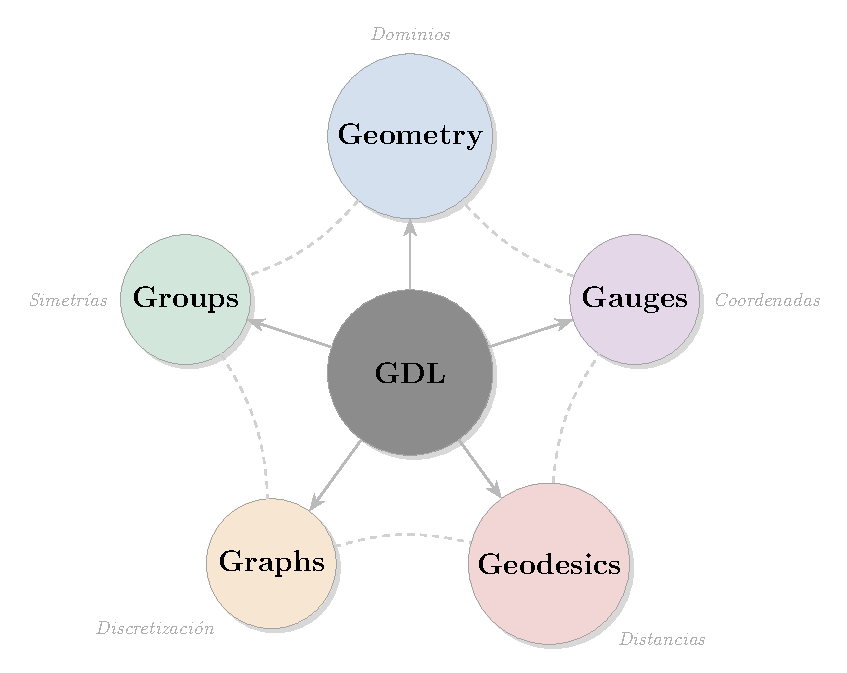
\includegraphics[width=0.7\textwidth]{images/five_gs_framework.pdf}
\caption[Las cinco G's del Geometric Deep Learning]{Las cinco G's fundamentales del Geometric Deep Learning. Cada componente representa un aspecto esencial del marco unificador: \textbf{Geometry} (dominios), \textbf{Groups} (simetrías), \textbf{Graphs} (discretización), \textbf{Geodesics} (distancias) y \textbf{Gauges} (coordenadas locales).}
\label{fig:five_gs_framework}
\end{figure}

La \autoref{fig:jerarquia_5gs} complementa esta visión mostrando la estructura jerárquica de las cinco Gs, desde la base más fundamental (la geometría del dominio) hasta los niveles más específicos de abstracción.

\begin{figure}[htbp]
\centering
\begin{tikzpicture}[scale=0.75]
% Definir estilos
\tikzset{
    level/.style={rectangle, rounded corners=3pt, draw, minimum width=2.8cm, minimum height=0.7cm, align=center, font=\small\bfseries},
    arrow/.style={->, thick, >=stealth, gray!70},
    desc/.style={font=\scriptsize, text=black!60, align=left}
}

% Niveles de la pirámide (de abajo hacia arriba)
\node[level, fill=gdlgreen!15, minimum width=10cm] (geom) at (0,0) {Geometría};
\node[level, fill=gdlgreen!25, minimum width=8cm] (grupos) at (0,1.2) {Grupos};
\node[level, fill=gdlgreen!35, minimum width=6cm] (grafos) at (0,2.4) {Grafos};
\node[level, fill=gdlgreen!45, minimum width=4cm] (geod) at (0,3.6) {Geodésicas};
\node[level, fill=gdlgreen!55, minimum width=2.5cm] (gauges) at (0,4.8) {Gauges};

% Flechas de relación
\draw[arrow] (geom.north) ++(0,0.1) -- ++(0,0.3);
\draw[arrow] (grupos.north) ++(0,0.1) -- ++(0,0.3);
\draw[arrow] (grafos.north) ++(0,0.1) -- ++(0,0.3);
\draw[arrow] (geod.north) ++(0,0.1) -- ++(0,0.3);

% Descripciones a la derecha (posiciones relativas al borde de cada nivel)
\node[desc, anchor=west] at (geom.east) {\quad Dominio $\Omega$ donde viven los datos};
\node[desc, anchor=west] at (grupos.east) {\quad Simetrías $G$ que preservan estructura};
\node[desc, anchor=west] at (grafos.east) {\quad Discretización del dominio};
\node[desc, anchor=west] at (geod.east) {\quad Propagación de información};
\node[desc, anchor=west] at (gauges.east) {\quad Invarianzas locales};

% Símbolos a la izquierda (posiciones relativas al borde de cada nivel)
\node[font=\scriptsize, anchor=east] at (geom.west) {$\mathbb{R}^n$, $\mathcal{M}$, $\mathcal{G}$\quad};
\node[font=\scriptsize, anchor=east] at (grupos.west) {$\text{SO}(n)$, $S_n$, $E(n)$\quad};
\node[font=\scriptsize, anchor=east] at (grafos.west) {$G=(V,E)$\quad};
\node[font=\scriptsize, anchor=east] at (geod.west) {$d(x,y)$, paths\quad};
\node[font=\scriptsize, anchor=east] at (gauges.west) {frames\quad};

\end{tikzpicture}
\caption[Jerarquía de las cinco Gs del GDL]{Estructura jerárquica de las cinco Gs del Geometric Deep Learning. Desde la base, la \textbf{Geometría} define el dominio donde residen los datos; los \textbf{Grupos} capturan las simetrías del problema; los \textbf{Grafos} discretizan el dominio; las \textbf{Geodésicas} determinan cómo se propaga la información; y los \textbf{Gauges} manejan las invarianzas locales en sistemas de coordenadas.}
\label{fig:jerarquia_5gs}
\end{figure}

Desde esta perspectiva unificadora, el \gls{GDL} establece que el procesamiento efectivo de señales sobre dominios geométricos requiere respetar tres principios fundamentales:

\begin{enumerate}
    \item \textbf{Localidad geométrica}: Las operaciones deben ser locales respecto a la métrica del dominio. Las arquitecturas geométricas explotan la estructura local mediante vecindarios definidos por la geometría subyacente, permitiendo que la información se propague de forma consistente con las distancias intrínsecas del espacio (véase \autoref{sec:grafos_discretizacion} para la formalización mediante grafos).

    \item \textbf{Equivarianza}: Las transformaciones deben preservar las simetrías relevantes del problema. Una función equivariante conmuta con las acciones del grupo de simetría, garantizando que transformaciones equivalentes de la entrada produzcan transformaciones correspondientes en la salida (véase Sección~\ref{subsec:equivarianza_invarianza} para la teoría completa).

    \item \textbf{Composicionalidad}: Las representaciones complejas se construyen jerárquicamente mediante composición de operaciones más simples. La composición de capas equivariantes preserva la equivarianza extremo a extremo (\autoref{theorem:equivariant_composition}), permitiendo arquitecturas profundas que mantienen las propiedades geométricas deseadas. Esta propiedad es fundamental para el Teorema de Aproximación Universal Equivariante (\autoref{theorem:universal_approximation_equivariant}), que garantiza el poder expresivo de las redes equivariantes.
\end{enumerate}

\section{Geometría: Los Dominios de los Datos}\label{sec:geometria_dominios}

Para diseñar arquitecturas neuronales efectivas en \gls{GDL}, debemos comprender la \textbf{geometría intrínseca} de los dominios (\autoref{def:dominio_datos}) donde residen los datos. Diferentes tipos de datos habitan naturalmente diferentes espacios geométricos, y reconocer y respetar estas geometrías resulta determinante para el éxito del Deep Learning. Los conceptos formales de simetría y equivarianza se desarrollan en la \autoref{sec:grupos_simetrias}.

La elección del dominio geométrico no es arbitraria ni meramente técnica: refleja la estructura intrínseca de los datos y determina qué operaciones son naturales y eficientes. Mientras que la tradición del Deep Learning ha favorecido representaciones vectoriales estándar (vectores, matrices, tensores en $\mathbb{R}^n$) en un espacio euclidiano, muchos datos reales poseen geometrías intrínsecas que estas representaciones no capturan adecuadamente. Las moléculas viven naturalmente en espacios con simetrías del grupo euclidiano $E(3)$, las jerarquías se representan mejor en espacios hiperbólicos $\mathbb{H}^n$, y las direcciones omnidireccionales habitan esferas $S^n$. Forzar estos datos a espacios euclidianos destruye información estructural valiosa y dificulta el aprendizaje efectivo.

\subsection{Geometría de los Datos}\label{subsec:geometria_datos}

En el \autoref{ch:neural_networks} establecimos el marco conceptual fundamental de señales sobre dominios estructurados (véase la \autoref{sec:datos_estructura}), donde introdujimos la distinción entre \textit{dominio} ($\Omega$), \textit{estructura} ($\mathcal{S}$), y \textit{señal} ($f$). Este marco nos permitió caracterizar formalmente diferentes tipos de datos mediante el triple $(\Omega, \mathcal{S}, f)$ o, equivalentemente, mediante el par geometría-atributos $(\mathcal{D}, f)$ donde $\mathcal{D} = (\Omega, \mathcal{S})$ representa la geometría del dominio y $f$ los atributos observados.

El concepto de \textit{geometría de los datos} profundiza en esta perspectiva, refiriéndose a las estructuras geométricas naturales que emergen de la naturaleza intrínseca de los datos, más allá de sus representaciones numéricas superficiales. El \gls{GDL} propone que estas geometrías intrínsecas $\mathcal{D} = (\Omega, \mathcal{S})$ no son meramente detalles de representación, sino propiedades fundamentales que determinan qué arquitecturas neuronales son apropiadas y efectivas para cada tipo de datos.

\paragraph{De representaciones euclidianas a estructuras geométricas complejas}

Tradicionalmente, el aprendizaje automático ha operado bajo el paradigma de que todos los datos pueden representarse como:

\begin{itemize}
    \item \textbf{Vectores}: $\mathbb{R}^n$ (secuencias, embeddings, características extraídas)
    \item \textbf{Matrices}: $\mathbb{R}^{n \times m}$ (imágenes en escala de grises, tablas de datos tabulares)
    \item \textbf{Tensores de orden superior}: $\mathbb{R}^{n_1 \times n_2 \times \cdots \times n_k}$ (imágenes RGB como $\mathbb{R}^{H \times W \times 3}$, video como $\mathbb{R}^{T \times H \times W \times 3}$)
\end{itemize}

Esta perspectiva simplificadora ha sido tremendamente exitosa. Sin embargo, esta visión es fundamentalmente limitada. Retomemos algunos de los ejemplos presentados en el \autoref{ch:neural_networks} para examinar las limitaciones de las representaciones euclidianas desde la perspectiva del \gls{GDL}:

\begin{itemize}
    \item \textbf{Moléculas como grafos 3D} (cf.~\autoref{ex:molecula}): Una molécula no es simplemente un conjunto de coordenadas atómicas en $\mathbb{R}^{3n}$. Como vimos anteriormente, su estructura combina \textit{conectividad discreta} (grafo de enlaces químicos covalentes) con \textit{geometría continua tridimensional} (posiciones espaciales de átomos). Más fundamentalmente, las propiedades físico-químicas son invariantes bajo el grupo euclidiano $E(3)$ de traslaciones, rotaciones y reflexiones. Vectorizar las coordenadas arbitrariamente rompe estas simetrías naturales y fuerza a las redes neuronales a reaprender invarianzas físicas fundamentales.

    \item \textbf{Redes sociales} (cf.~\autoref{ex:red_social}): Un grafo social $G = (V, E)$ carece de orden natural entre sus nodos. Asignar índices $\{1, 2, \ldots, n\}$ a los usuarios e intentar representar el grafo como una matriz de adyacencia $A \in \mathbb{R}^{n \times n}$ introduce un orden completamente artificial. La estructura relevante es puramente topológica: quién está conectado con quién, no en qué ``posición'' está cada usuario.

    \item \textbf{Superficies físicas} (cf.~\autoref{ex:superficie_riemanniana}): Una superficie 3D (la corteza cerebral, la superficie de una proteína, un objeto escaneado) es naturalmente una variedad riemanniana 2D embebida en $\mathbb{R}^3$. Las distancias geodésicas sobre la superficie y la curvatura intrínseca son propiedades geométricas fundamentales independientes de cómo parametricemos o triangulemos la superficie. Una malla triangular con $n$ vértices no es simplemente un tensor $\mathbb{R}^{n \times 3}$ de coordenadas: es una discretización de una variedad continua subyacente.
\end{itemize}

Estos ejemplos ilustran un principio fundamental: los datos poseen geometrías intrínsecas que las representaciones vectoriales estándar no capturan completamente. El \gls{GDL} propone un cambio de paradigma: en lugar de forzar todos los datos a $\mathbb{R}^n$, debemos diseñar arquitecturas que operen directamente sobre las geometrías naturales de los datos.

\subsection{Geometría Euclidiana Tradicional}\label{subsec:geometria_euclidiana}

Para poder entender las diferencias entre las geometrías debemos primero entender la geometría euclidiana tradicional. El espacio euclidiano $\mathbb{R}^n$ constituye el dominio geométrico más familiar y ampliamente utilizado en el Deep Learning clásico. Su ubicuidad no es accidental: la estructura euclidiana proporciona simplicidad computacional, herramientas analíticas bien desarrolladas, y representaciones uniformes que han demostrado ser efectivas en muchas aplicaciones.

\paragraph{Los postulados de Euclides}

La geometría euclidiana se fundamenta en los cinco postulados establecidos por Euclides en sus \textit{Elementos} \citep{euclid1956elements}. Estos axiomas definen las propiedades fundamentales del espacio plano:

\begin{enumerate}
    \item \textbf{Postulado de la recta}: Por dos puntos distintos pasa exactamente una recta.
    \item \textbf{Postulado del segmento}: Todo segmento puede extenderse indefinidamente en una línea recta.
    \item \textbf{Postulado del círculo}: Dado un punto y una distancia, se puede trazar un círculo con centro en ese punto y radio igual a esa distancia.
    \item \textbf{Postulado de los ángulos rectos}: Todos los ángulos rectos son iguales entre sí.
    \item \textbf{Postulado de las paralelas}: Por un punto exterior a una recta, pasa exactamente una recta paralela a la primera.
\end{enumerate}

El quinto postulado, conocido como \textit{postulado de las paralelas} o \textit{postulado de Euclides}, es históricamente el más controvertido. Durante más de dos milenios, matemáticos intentaron demostrarlo a partir de los otros cuatro, hasta que en el siglo XIX Gauss, Bolyai y Lobachevsky demostraron independientemente que negarlo produce geometrías consistentes: las \textit{geometrías no euclidianas} \citep{gray2007worlds}.

\paragraph{Formalización matemática moderna}

Intuitivamente, la \textit{geometría euclidiana} es aquella que utiliza la métrica euclidiana, o norma $\ell^2$, para medir distancias

\[
d(\mathbf{x}, \mathbf{y}) = \|\mathbf{x} - \mathbf{y}\|_2 = \sqrt{\sum_{i=1}^n (x_i - y_i)^2}
\]

Esta métrica define nociones de distancia, vecindad y continuidad que son uniformes y bien comportadas: satisface las propiedades que esperamos del espacio ``plano'' cotidiano: los caminos más cortos son líneas rectas, los triángulos tienen ángulos que suman $\pi$, y las rectas paralelas permanecen equidistantes. Además, las operaciones fundamentales (productos internos, proyecciones, convoluciones) tienen formas cerradas eficientes y propiedades analíticas bien comprendidas.

En el lenguaje de la geometría diferencial moderna, el espacio euclidiano $\mathbb{R}^n$ es una variedad riemanniana (\autoref{def:metrica_riemanniana} y \autoref{subsec:variedades_riemannianas}) con las siguientes propiedades características (los conceptos referenciados se desarrollan formalmente más adelante en este capítulo):

\begin{itemize}
    \item \textbf{Métrica riemanniana plana}: La métrica riemanniana $g$ es constante e igual a la identidad ($g_{ij} = \delta_{ij}$), lo que induce la distancia euclidiana estándar (véase \autoref{subsec:variedades_riemannianas}).
    \item \textbf{Curvatura cero}: La curvatura seccional (\autoref{def:curvatura_preliminar}) es $K = 0$ en todo punto y dirección.
    \item \textbf{Geodésicas rectas}: Las geodésicas (\autoref{def:geodesica}) son líneas rectas, formalizando los postulados 1 y 2 de Euclides.
    \item \textbf{Grupo de simetrías}: El grupo de isometrías es el \textit{grupo euclidiano} $E(n) = \mathbb{R}^n \rtimes O(n)$ (\autoref{def:grupo}, \autoref{def:producto_semidirecto}), que incluye rotaciones, reflexiones y traslaciones combinadas mediante el producto semidirecto.
\end{itemize}

La conexión profunda entre la geometría clásica de Euclides y la geometría diferencial moderna se establece mediante el siguiente resultado fundamental (véase la \autoref{sec:gauss_bonnet} del Apéndice~\ref{ch:teoremas_complementarios} para el teorema generalizado y su demostración):

\begin{theorem}[Gauss-Bonnet para triángulos geodésicos]\label{thm:gauss_bonnet_triangulo}
Sea $\mathcal{M}$ una superficie riemanniana con curvatura gaussiana $K$, y sea $T \subset \mathcal{M}$ un triángulo geodésico con ángulos interiores $\alpha$, $\beta$, $\gamma$. Entonces:
\begin{equation}\label{eq:gauss_bonnet_triangulo}
\alpha + \beta + \gamma = \pi + \int_T K \, dA
\end{equation}
donde $dA$ denota el elemento de área inducido por la métrica riemanniana.
\end{theorem}

Este teorema \citep{lee2018introduction} tiene una consecuencia fundamental: cuando $K = 0$ (curvatura cero), recuperamos el resultado euclidiano clásico de que los ángulos de un triángulo suman exactamente $\pi$. Más aún, el teorema demuestra que el quinto postulado de Euclides (paralelas) es \textit{equivalente} a la condición de curvatura gaussiana $K = 0$.

\paragraph{Limitaciones de la geometría euclidiana}

Sin embargo, la geometría euclidiana no es universal. Cuando los datos tienen estructura intrínsecamente no-euclidiana, forzarlos a representaciones vectoriales/matriciales estándar destruye información estructural importante:

\begin{itemize}
    \item \textbf{Imágenes esféricas} (panoramas $360^\circ$): Viven naturalmente en la esfera $S^2$, pero la proyección equirectangular a $\mathbb{R}^{H \times W}$ introduce distorsiones extremas en los polos. La distancia $\ell^2$ entre píxeles no respeta las distancias geodésicas sobre $S^2$. Las rotaciones en $SO(3)$ se vuelven transformaciones complejas y no lineales en la representación matricial.

    \item \textbf{Nubes de puntos 3D} (cf.~\autoref{ex:nube_puntos}): Conjuntos $\{p_1, \ldots, p_n\} \subset \mathbb{R}^3$ sin orden canónico. Vectorizarlos forzadamente a $\mathbb{R}^{3n}$ impone un orden arbitrario que no es intrínseco al objeto geométrico, violando la invarianza permutacional natural.

    \item \textbf{Estructuras moleculares}: Tienen geometría tridimensional compleja con simetrías del grupo euclidiano $E(3)$. Representarlas como vectores en $\mathbb{R}^d$ rompe las invarianzas físicas fundamentales bajo rotaciones y traslaciones.

    \item \textbf{Datos jerárquicos}: Naturalmente viven en espacios hiperbólicos $\mathbb{H}^n$ donde la distancia captura jerarquía. Embeddings en $\mathbb{R}^n$ euclidiano requieren dimensionalidad exponencialmente mayor para preservar distancias \citep{nickel2017poincare}.
\end{itemize}

\subsection{Fundamentos de Variedades}\label{subsec:fundamentos_variedades}

Para formalizar la idea de que los datos residen en espacios con geometría intrínseca, necesitamos el concepto matemático de \textit{variedad}. Esta subsección desarrolla los fundamentos necesarios, comenzando con preliminares topológicos y progresando hacia variedades diferenciables.

\subsubsection{Preliminares topológicos}\label{subsubsec:preliminares_topologicos}

Antes de introducir el concepto de variedad, necesitamos establecer los fundamentos topológicos necesarios. Para una exposición completa de estos conceptos, véase~\citet{munkres2000topology}.

\begin{definition}[Espacio topológico]\label{def:espacio_topologico}
Un \textit{espacio topológico} es un par $(X, \tau)$ donde $X$ es un conjunto y $\tau$ es una colección de subconjuntos de $X$ (llamados \textbf{conjuntos abiertos}) que satisface:
\begin{enumerate}
	\item $\emptyset, X \in \tau$ (el vacío y el total son abiertos)
	\item La unión arbitraria de conjuntos abiertos es abierta: si $\{U_\alpha\}_{\alpha \in I} \subset \tau$, entonces $\bigcup_{\alpha \in I} U_\alpha \in \tau$
	\item La intersección finita de conjuntos abiertos es abierta: si $U_1, \ldots, U_n \in \tau$, entonces $\bigcap_{i=1}^n U_i \in \tau$
\end{enumerate}
La colección $\tau$ se denomina \textbf{topología} en $X$.
\end{definition}

\begin{definition}[Espacio de Hausdorff]\label{def:espacio_hausdorff}
Un espacio topológico $(X, \tau)$ es un \textit{espacio de Hausdorff} (o $T_2$) si para cualesquiera dos puntos distintos $x, y \in X$ con $x \neq y$, existen abiertos disjuntos $U, V \in \tau$ tales que $x \in U$, $y \in V$ y $U \cap V = \emptyset$.

Intuitivamente, esto significa que los puntos pueden ``separarse'' mediante conjuntos abiertos.
\end{definition}

\begin{definition}[Base numerable]\label{def:base_numerable}
Un espacio topológico $(X, \tau)$ tiene \textit{base numerable} (o satisface el segundo axioma de numerabilidad) si existe una colección numerable $\mathcal{B} = \{B_n\}_{n \in \mathbb{N}}$ de conjuntos abiertos tal que todo abierto de $\tau$ puede expresarse como unión de elementos de $\mathcal{B}$.

Formalmente, $\mathcal{B} \subset \tau$ es base si para todo $U \in \tau$ y todo $x \in U$, existe $B \in \mathcal{B}$ tal que $x \in B \subseteq U$.
\end{definition}

\begin{definition}[Homeomorfismo]\label{def:homeomorfismo}
Sean $(X, \tau_X)$ y $(Y, \tau_Y)$ espacios topológicos. Una función $f: X \to Y$ es un \textit{homeomorfismo} si:
\begin{enumerate}
	\item $f$ es biyectiva
	\item $f$ es continua: para todo $V \in \tau_Y$, se tiene $f^{-1}(V) \in \tau_X$
	\item $f^{-1}$ es continua: para todo $U \in \tau_X$, se tiene $(f^{-1})^{-1}(U) = f(U) \in \tau_Y$
\end{enumerate}
Dos espacios son \textit{homeomorfos} si existe un homeomorfismo entre ellos. Intuitivamente, son ``topológicamente idénticos''.
\end{definition}

\subsubsection{Variedades topológicas}\label{subsubsec:variedades_topologicas}

Con estos conceptos establecidos, podemos ahora definir rigurosamente las variedades topológicas. Para un desarrollo completo de la teoría de variedades, recomendamos~\citet{lee2012introduction}.

\begin{definition}[Variedad topológica]\label{def:variedad_topologica}
Una \textit{variedad topológica} de dimensión $m$ es un espacio topológico $\mathcal{M}$ que satisface:
\begin{enumerate}
	\item $\mathcal{M}$ es un espacio de Hausdorff
	\item $\mathcal{M}$ tiene base numerable
	\item $\mathcal{M}$ es localmente euclidiano de dimensión $m$: para todo punto $p \in \mathcal{M}$, existe un entorno abierto $U \ni p$ y un homeomorfismo $\phi: U \to V$ donde $V$ es un abierto de $\mathbb{R}^m$
\end{enumerate}
\end{definition}

Intuitivamente, una variedad es un espacio que localmente ``se parece'' al espacio euclidiano, aunque globalmente puede tener una estructura muy diferente. Podemos ilustrarlo con los siguientes ejemplos:

\begin{itemize}
    \item \textbf{La Tierra como variedad 2D}: Aunque sabemos que la Tierra es aproximadamente esférica, cuando caminamos por una ciudad, localmente percibimos el suelo como plano. Este es precisamente el concepto de variedad: un espacio que globalmente puede ser curvo, pero localmente se comporta como el espacio euclidiano familiar.
    \item \textbf{Una hoja de papel arrugada}: Si arrugamos una hoja, sigue siendo localmente bidimensional (podemos poner un dedo en cualquier punto y moverlo en dos direcciones independientes), pero globalmente tiene una forma compleja en el espacio tridimensional.
    \item \textbf{El espacio de configuraciones de un robot}: Un brazo robótico con múltiples articulaciones tiene un espacio de configuraciones que no es euclidiano, pero localmente podemos parametrizar las posiciones cercanas con coordenadas estándar.
\end{itemize}

Esta intuición es crucial porque muchos conjuntos de datos de alta dimensión (imágenes, texto, señales) realmente ``viven'' en variedades de dimensión mucho menor, y explotarlo mejora significativamente el aprendizaje.

\begin{definition}[Atlas y cartas]\label{def:atlas_cartas}
Un \textit{atlas} de dimensión $m$ para un espacio topológico $\mathcal{M}$ es una colección $\mathcal{A} = \{(U_\alpha, \phi_\alpha)\}_{\alpha \in I}$ donde:
\begin{itemize}
	\item $\{U_\alpha\}_{\alpha \in I}$ es un cubrimiento abierto de $\mathcal{M}$
	\item Cada $\phi_\alpha: U_\alpha \to V_\alpha \subset \mathbb{R}^m$ es un homeomorfismo (llamado \textit{carta})
\end{itemize}

Las funciones de transición $\phi_\beta \circ \phi_\alpha^{-1}: \phi_\alpha(U_\alpha \cap U_\beta) \to \phi_\beta(U_\alpha \cap U_\beta)$ determinan la estructura de la variedad.
\end{definition}

\begin{figure}[htbp]
\centering
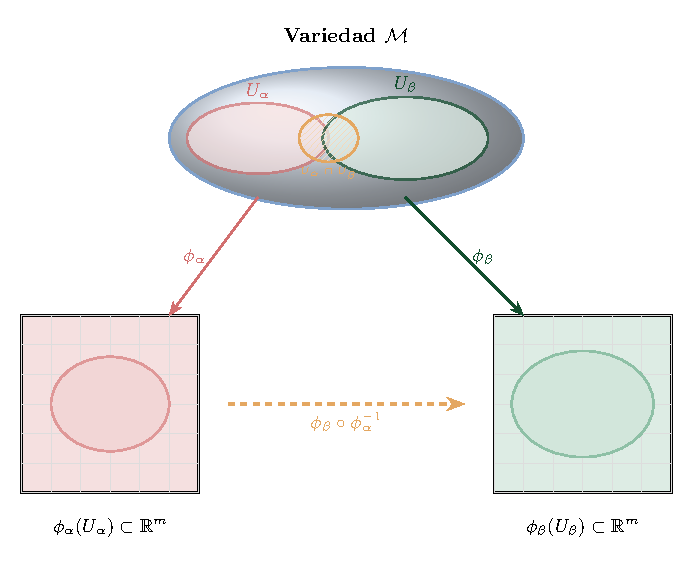
\includegraphics[width=0.75\textwidth]{images/charts_atlas.pdf}
\caption[Atlas y cartas de una variedad]{Atlas $\mathcal{A} = \{(U_\alpha, \phi_\alpha)\}_{\alpha \in I}$ de una variedad $\mathcal{M}$: cada carta $(U_\alpha, \phi_\alpha)$ es un homeomorfismo $\phi_\alpha: U_\alpha \to V_\alpha \subset \mathbb{R}^m$ que define coordenadas locales en un abierto de $\mathcal{M}$. La función de transición $\phi_\beta \circ \phi_\alpha^{-1}: \phi_\alpha(U_\alpha \cap U_\beta) \to \phi_\beta(U_\alpha \cap U_\beta)$ conecta las representaciones de cartas solapadas.}
\label{fig:charts_atlas}
\end{figure}

\subsubsection{Variedades diferenciables y espacio tangente}\label{subsubsec:variedades_diferenciables}

\begin{definition}[Función suave]\label{def:funcion_suave}
Sea $U \subseteq \mathbb{R}^n$ un abierto. Una función $f: U \rightarrow \mathbb{R}^m$ es \textit{suave} (o de \textit{clase $C^\infty$}) si posee derivadas parciales continuas de todos los órdenes.
\end{definition}

Más generalmente, una función entre variedades diferenciables es suave si su expresión en coordenadas locales es suave.

\begin{definition}[Variedad diferenciable]\label{def:variedad_diferenciable}
Una variedad topológica $\mathcal{M}$ es \textit{diferenciable} (o suave) si posee un atlas $\mathcal{A} = \{(U_\alpha, \phi_\alpha)\}$ tal que todas sus cartas $\phi_\beta \circ \phi_\alpha^{-1}$ son de clase $C^\infty$.
\end{definition}

La estructura diferenciable permite definir conceptos del cálculo (derivadas, integrales, ecuaciones diferenciales) en la variedad. El concepto más fundamental es el de \textit{espacio tangente}, que captura la noción de ``direcciones infinitesimales'' en cada punto. Presentamos dos construcciones equivalentes que ofrecen perspectivas complementarias.

\begin{definition}[Espacio tangente vía curvas]\label{def:espacio_tangente_curvas}
Sea $\mathcal{M}$ una variedad diferenciable y $p \in \mathcal{M}$. Dos curvas $\gamma_1, \gamma_2: (-\epsilon, \epsilon) \to \mathcal{M}$ con $\gamma_1(0) = \gamma_2(0) = p$ se dicen \textit{tangentes en $p$} si para alguna (y por tanto toda) carta $(U, \phi)$ con $p \in U$:
\[
\frac{d}{dt}\bigg|_{t=0} (\phi \circ \gamma_1)(t) = \frac{d}{dt}\bigg|_{t=0} (\phi \circ \gamma_2)(t)
\]
El \textit{espacio tangente} $T_p\mathcal{M}$ es el conjunto de clases de equivalencia $[\gamma]$ de curvas tangentes en $p$.
\end{definition}

Esta definición captura la intuición geométrica: un vector tangente representa una ``dirección de movimiento'' desde el punto $p$, determinada por la velocidad inicial de cualquier curva que pase por $p$ en esa dirección.

\begin{remark}[Estructura de espacio vectorial]\label{rem:estructura_vectorial_curvas}
El conjunto $T_p^{\text{curvas}}\mathcal{M}$ admite una estructura de espacio vectorial inducida por cualquier carta $(U, \phi)$ con $p \in U$. La aplicación $[\gamma] \mapsto (\phi \circ \gamma)'(0) \in \mathbb{R}^m$ es una biyección entre $T_p^{\text{curvas}}\mathcal{M}$ y $\mathbb{R}^m$, y \textit{transportamos} la estructura vectorial de $\mathbb{R}^m$ a $T_p^{\text{curvas}}\mathcal{M}$ mediante esta biyección. Es decir, definimos:
\[
\alpha[\gamma_1] + [\gamma_2] \;=\; \bigl[\gamma\bigr], \quad \text{donde $(\phi \circ \gamma)'(0) = \alpha(\phi \circ \gamma_1)'(0) + (\phi \circ \gamma_2)'(0)$}.
\]
Esta estructura es \textit{independiente de la carta} elegida: si $(V, \psi)$ es otra carta con $p \in V$, la regla de la cadena aplicada a la función de transición $\psi \circ \phi^{-1}$ garantiza que el isomorfismo inducido por $\psi$ es compatible con el inducido por $\phi$.
\end{remark}

\begin{definition}[Espacio tangente vía derivaciones]\label{def:espacio_tangente_derivaciones}
Sea $\mathcal{M}$ una variedad diferenciable y $p \in \mathcal{M}$. Una \textit{derivación en $p$} es una aplicación lineal $v: C^\infty(\mathcal{M}) \to \mathbb{R}$ que satisface la regla de Leibniz para todas $f, g \in C^\infty(\mathcal{M})$:
\[
v(fg) = v(f)g(p) + f(p)v(g)
\]
El \textit{espacio tangente} $T_p\mathcal{M}$ es el espacio vectorial de todas las derivaciones en $p$.
\end{definition}

Esta definición algebraica captura la idea de que un vector tangente es un ``operador de derivada direccional'': dado un vector $v$ y una función $f$, $v(f)$ representa la tasa de cambio de $f$ en la dirección $v$.

\begin{lemma}[Descomposición de derivaciones en coordenadas]\label{lem:descomposicion_derivaciones}
Sea $\mathcal{M}$ una variedad diferenciable de dimensión $m$, $p \in \mathcal{M}$ y $(U, \phi)$ una carta con $\phi(p) = 0$ y funciones coordenadas $x^1, \ldots, x^m$. Entonces:
\begin{enumerate}
	\item Las derivaciones son operadores locales: si $f = g$ en un entorno de $p$, entonces $v(f) = v(g)$ para toda derivación $v$ en $p$. Esto permite evaluar $v$ sobre funciones definidas solo en $U$, extendiéndolas a $\mathcal{M}$ mediante funciones de corte (bump functions), con resultado independiente de la extensión.
	\item Toda derivación $v$ en $p$ se expresa como:
	\[
	v = \sum_{j=1}^{m} v(x^j) \frac{\partial}{\partial x^j}\bigg|_p
	\]
	donde $\frac{\partial}{\partial x^j}\big|_p(f) = \frac{\partial(f \circ \phi^{-1})}{\partial x^j}\big|_{\phi(p)}$. En particular, $\dim T_p^{\text{deriv}}\mathcal{M} = m$.
\end{enumerate}
\end{lemma}

\begin{proof}
\textbf{(1) Localidad.} Sea $\chi \in C^\infty(\mathcal{M})$ una bump function con $\chi \equiv 1$ en un entorno $W \subset U$ de $p$ y $\operatorname{supp}(\chi) \subset U$. Si $f = g$ en $U$, entonces $\chi(f - g) = 0$ en todo $\mathcal{M}$. Por la regla de Leibniz, $0 = v(\chi(f-g)) = v(\chi)(f-g)(p) + \chi(p) \, v(f-g) = v(f-g)$, ya que $\chi(p) = 1$ y $(f-g)(p) = 0$.

\textbf{(2) Descomposición.} Primero, toda derivación anula constantes: si $c \in \mathbb{R}$, entonces $v(c) = v(c \cdot 1) = c \, v(1)$ y $v(1) = v(1 \cdot 1) = v(1) \cdot 1 + 1 \cdot v(1) = 2v(1)$, de donde $v(1) = 0$ y por tanto $v(c) = 0$.

Sea $f \in C^\infty(\mathcal{M})$. Escribimos $\hat{f} = f \circ \phi^{-1}: \phi(U) \to \mathbb{R}$. Por el teorema fundamental del cálculo con resto integral, para $\mathbf{x} = (x^1, \ldots, x^m)$ en un entorno convexo de $0 \in \phi(U)$:
\[
\hat{f}(\mathbf{x}) = \hat{f}(0) + \sum_{j=1}^{m} x^j \, g_j(\mathbf{x}), \quad \text{donde } g_j(\mathbf{x}) = \int_0^1 \frac{\partial \hat{f}}{\partial x^j}(t\mathbf{x}) \, dt
\]
Las funciones $g_j$ son suaves y $g_j(0) = \frac{\partial \hat{f}}{\partial x^j}(0)$. Componiendo con $\phi$ y usando localidad (apartado 1), obtenemos en $U$:
\[
f = f(p) + \sum_{j=1}^{m} x^j \cdot (g_j \circ \phi)
\]
donde identificamos $x^j$ con la función coordenada $x^j = \pi^j \circ \phi$. Aplicando $v$ y usando que $v$ anula constantes, $x^j(p) = 0$ y la regla de Leibniz:
\[
v(f) = \sum_{j=1}^{m} \bigl[v(x^j) \cdot g_j(\phi(p)) + x^j(p) \cdot v(g_j \circ \phi)\bigr] = \sum_{j=1}^{m} v(x^j) \frac{\partial(f \circ \phi^{-1})}{\partial x^j}\bigg|_{0}
\]
Esto muestra que $v = \sum_j v(x^j) \frac{\partial}{\partial x^j}\big|_p$. Como $\frac{\partial}{\partial x^j}\big|_p(x^k) = \delta_j^k$, las derivaciones $\{\frac{\partial}{\partial x^j}\big|_p\}_{j=1}^m$ son linealmente independientes y generan $T_p^{\text{deriv}}\mathcal{M}$ \citep[Proposition 3.2]{lee2012introduction}.
\end{proof}

\begin{proposition}[Equivalencia de las definiciones de espacio tangente]\label{prop:equivalencia_espacio_tangente}
Las dos definiciones de espacio tangente son canónicamente isomorfas (el isomorfismo es independiente de la elección de coordenadas). El isomorfismo $\Phi: T_p^{\text{curvas}}\mathcal{M} \to T_p^{\text{deriv}}\mathcal{M}$ está dado por:
\[
\Phi([\gamma])(f) = \frac{d}{dt}\bigg|_{t=0} (f \circ \gamma)(t)
\]
para toda función $f \in C^\infty(\mathcal{M})$.
\end{proposition}

\begin{proof}
Procedemos en cuatro pasos: verificamos que $\Phi$ está bien definida, que su imagen son derivaciones, y que es biyectiva.

\textbf{Paso 1: $\Phi$ está bien definida.} Sean $\gamma_1, \gamma_2$ dos curvas con $\gamma_1(0) = \gamma_2(0) = p$ y $\gamma_1 \sim \gamma_2$ (es decir, son tangentes en $p$). Debemos mostrar que $\Phi([\gamma_1]) = \Phi([\gamma_2])$. Sea $(U, \phi)$ una carta local en $p$ con $\phi = (x^1, \ldots, x^m)$. Por definición de tangencia, $(\phi \circ \gamma_1)'(0) = (\phi \circ \gamma_2)'(0)$. Para cualquier $f \in C^\infty(\mathcal{M})$, factorizamos $f \circ \gamma_i = (f \circ \phi^{-1}) \circ (\phi \circ \gamma_i)$ y aplicamos la regla de la cadena:
\[
(f \circ \gamma_i)'(0) = \sum_{j=1}^{m} \frac{\partial (f \circ \phi^{-1})}{\partial x^j}\bigg|_{\phi(p)} \cdot (x^j \circ \gamma_i)'(0)
\]
Como $(x^j \circ \gamma_i)'(0)$ es la $j$-ésima componente de $(\phi \circ \gamma_i)'(0)$ y $(\phi \circ \gamma_1)'(0) = (\phi \circ \gamma_2)'(0)$, concluimos que $(f \circ \gamma_1)'(0) = (f \circ \gamma_2)'(0)$.

\textbf{Paso 2: $\Phi([\gamma])$ es una derivación.} Sea $v_\gamma = \Phi([\gamma])$. Verificamos las dos propiedades:
\begin{itemize}
    \item \textit{Linealidad}: Para $f, g \in C^\infty(\mathcal{M})$ y $\alpha, \beta \in \mathbb{R}$:
    \begin{align*}
    v_\gamma(\alpha f + \beta g) &= \frac{d}{dt}\bigg|_{t=0} (\alpha f + \beta g)(\gamma(t)) \\
    &= \alpha \frac{d}{dt}\bigg|_{t=0} f(\gamma(t)) + \beta \frac{d}{dt}\bigg|_{t=0} g(\gamma(t)) = \alpha v_\gamma(f) + \beta v_\gamma(g)
    \end{align*}
    \item \textit{Regla de Leibniz}: Para $f, g \in C^\infty(\mathcal{M})$, aplicamos la regla del producto para funciones reales de variable real $t \mapsto f(\gamma(t))$ y $t \mapsto g(\gamma(t))$:
    \begin{align*}
    v_\gamma(fg) &= \frac{d}{dt}\bigg|_{t=0} \bigl[f(\gamma(t)) \cdot g(\gamma(t))\bigr] \\
    &= \left(\frac{d}{dt}\bigg|_{t=0} f(\gamma(t))\right) g(\gamma(0)) + f(\gamma(0)) \left(\frac{d}{dt}\bigg|_{t=0} g(\gamma(t))\right) \\
    &= v_\gamma(f) \, g(p) + f(p) \, v_\gamma(g)
    \end{align*}
\end{itemize}

\textbf{Paso 3: $\Phi$ es inyectiva.} Supongamos que $\Phi([\gamma_1]) = \Phi([\gamma_2])$, es decir, que para toda $f \in C^\infty(\mathcal{M})$ se tiene $(f \circ \gamma_1)'(0) = (f \circ \gamma_2)'(0)$. Sea $(U, \phi)$ una carta con $p \in U$ y funciones coordenadas $x^j = \pi^j \circ \phi$, donde $\pi^j: \mathbb{R}^m \to \mathbb{R}$ es la proyección $j$-ésima. Las funciones $x^j$ están definidas en $U$, pero por localidad de $\Phi([\gamma])$ (véase el \autoref{lem:descomposicion_derivaciones}), podemos evaluarlas. Tomando $f = x^j$, obtenemos $(x^j \circ \gamma_1)'(0) = (x^j \circ \gamma_2)'(0)$ para todo $j = 1, \ldots, m$. Esto implica $(\phi \circ \gamma_1)'(0) = (\phi \circ \gamma_2)'(0)$, es decir, $\gamma_1 \sim \gamma_2$.

\textbf{Paso 4: $\Phi$ es sobreyectiva.} Sea $v \in T_p^{\text{deriv}}\mathcal{M}$ una derivación arbitraria. Sea $(U, \phi)$ una carta con $\phi(p) = 0$ y funciones coordenadas $x^1, \ldots, x^m$. Definimos el vector $\mathbf{a} = (a^1, \ldots, a^m) \in \mathbb{R}^m$ por $a^j = v(x^j)$ y consideremos la curva $\gamma(t) = \phi^{-1}(t\mathbf{a}) = \phi^{-1}(ta^1, \ldots, ta^m)$. Entonces $\gamma(0) = \phi^{-1}(0) = p$ y para cualquier $f \in C^\infty(\mathcal{M})$, la regla de la cadena da:
\[
\Phi([\gamma])(f) = \frac{d}{dt}\bigg|_{t=0} (f \circ \phi^{-1})(t\mathbf{a}) = \sum_{j=1}^{m} a^j \frac{\partial (f \circ \phi^{-1})}{\partial x^j}\bigg|_{0} = \sum_{j=1}^{m} v(x^j) \frac{\partial}{\partial x^j}\bigg|_p (f)
\]
Por el \autoref{lem:descomposicion_derivaciones}, $v = \sum_{j=1}^{m} v(x^j) \frac{\partial}{\partial x^j}\big|_p$, de donde $\Phi([\gamma]) = v$.
\end{proof}

\textbf{Intuición sobre las dos construcciones.} Las dos construcciones ofrecen perspectivas complementarias:
\begin{itemize}
	\item \textbf{Curvas}: Capturan la idea geométrica de ``direcciones de movimiento''. Son intuitivas para visualizar vectores tangentes como velocidades de partículas moviéndose sobre la variedad.
	\item \textbf{Derivaciones}: Capturan la idea analítica de ``direcciones de cambio de funciones''. Son convenientes para cálculos y generalizan naturalmente a espacios más abstractos.
\end{itemize}
En la práctica, usamos ambas según convenga: curvas para intuición geométrica, derivaciones para manipulaciones algebraicas.

\begin{example}[Espacio tangente a la esfera]\label{ex:espacio_tangente_esfera}
Considere la esfera $S^2 = \{(x,y,z) \in \mathbb{R}^3 : x^2 + y^2 + z^2 = 1\}$. En el polo norte $p = (0,0,1)$:
\begin{itemize}
	\item \textbf{Vía curvas}: Un vector tangente es la velocidad inicial de cualquier curva sobre $S^2$ que pase por $p$. Por ejemplo, $\gamma(t) = (\sin t, 0, \cos t)$ tiene $\gamma(0) = p$ y $\gamma'(0) = (1, 0, 0)$.
	\item \textbf{Vía derivaciones}: En coordenadas estereográficas $(u,v)$ centradas en $p$, las derivaciones $\partial/\partial u$ y $\partial/\partial v$ forman una base.
\end{itemize}
El espacio tangente $T_p S^2$ es el plano $\{(x,y,0) : x,y \in \mathbb{R}\}$, que es horizontal y tangente a la esfera en el polo norte.
\end{example}

\begin{figure}[htbp]
\centering
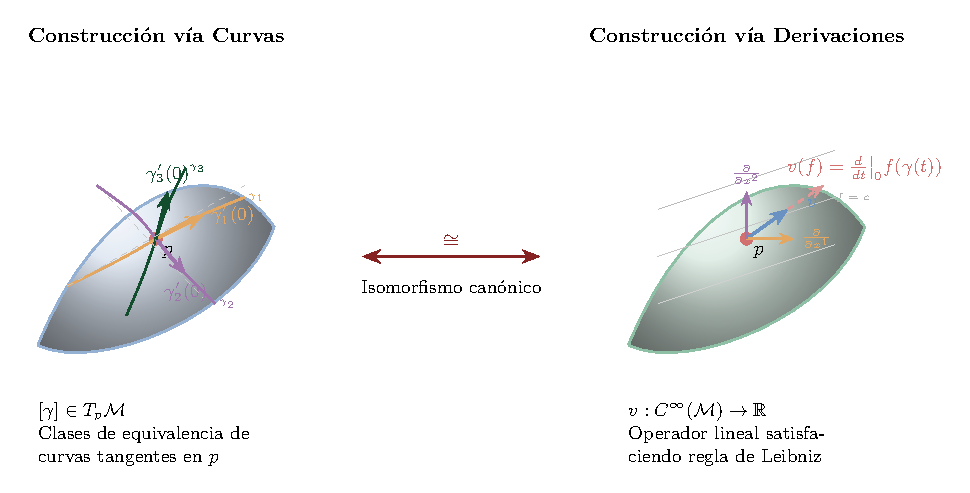
\includegraphics[width=0.7\textwidth]{images/tangent_space.pdf}
\caption[Espacio tangente a una variedad]{Espacio tangente $T_p\mathcal{M}$ en un punto $p$ de una variedad. Los vectores tangentes representan velocidades iniciales de curvas que pasan por $p$, formando un espacio vectorial que aproxima linealmente la variedad en cada punto.}
\label{fig:tangent_space}
\end{figure}

\begin{definition}[Diferencial de una aplicación suave]\label{def:diferencial_aplicacion_suave}
Sea $F: \mathcal{M} \to \mathcal{N}$ una aplicación suave entre variedades diferenciables. Para cada $p \in \mathcal{M}$, el \textit{diferencial} (o \textit{pushforward}) de $F$ en $p$ es la aplicación lineal $dF_p: T_p\mathcal{M} \to T_{F(p)}\mathcal{N}$ definida, en la formulación por derivaciones (\autoref{def:espacio_tangente_derivaciones}), por:
\[
dF_p(v)(g) = v(g \circ F) \quad \text{para toda } g \in C^\infty(\mathcal{N}).
\]
Si $(U, \phi)$ y $(V, \psi)$ son cartas locales en $p$ y $F(p)$ respectivamente, la expresión en coordenadas de $dF_p$ es la matriz jacobiana $\left(\frac{\partial (\psi \circ F \circ \phi^{-1})^i}{\partial x^j}\right)_{i,j}$.
\end{definition}

\begin{definition}[Inmersión suave]\label{def:inmersion_suave}
Una aplicación suave $F: \mathcal{M} \to \mathcal{N}$ es una \textit{inmersión} si su diferencial $dF_p: T_p\mathcal{M} \to T_{F(p)}\mathcal{N}$ es inyectiva para todo $p \in \mathcal{M}$. Equivalentemente, $\operatorname{rango}(dF_p) = \dim \mathcal{M}$ en cada punto.
\end{definition}

\begin{definition}[Submersión suave]\label{def:submersion_suave}
Una aplicación suave $F: \mathcal{M} \to \mathcal{N}$ es una \textit{submersión} si su diferencial $dF_p: T_p\mathcal{M} \to T_{F(p)}\mathcal{N}$ es suryectiva para todo $p \in \mathcal{M}$. Equivalentemente, $\operatorname{rango}(dF_p) = \dim \mathcal{N}$ en cada punto, lo cual requiere $\dim \mathcal{M} \geq \dim \mathcal{N}$.
\end{definition}

\begin{remark}\label{rem:inmersion_submersion_dualidad}
La inmersión y la submersión son nociones duales: la primera exige que $dF_p$ sea inyectiva ($\operatorname{rango} = \dim \mathcal{M}$, necesitando $\dim \mathcal{M} \leq \dim \mathcal{N}$), mientras que la segunda exige suryectividad ($\operatorname{rango} = \dim \mathcal{N}$, necesitando $\dim \mathcal{M} \geq \dim \mathcal{N}$). El Teorema del Nivel Regular (\autoref{thm:nivel_regular} del \autoref{ch:teoremas_complementarios}) garantiza que, si $F$ es una submersión, cada fibra $F^{-1}(q)$ es una subvariedad suave de $\mathcal{M}$ de dimensión $\dim \mathcal{M} - \dim \mathcal{N}$. Esta propiedad de las fibras como subvariedades será fundamental en la teoría de fibrados principales (\autoref{subsec:fibrados_principales}), donde la proyección $\pi: P \to \mathcal{M}$ es una submersión suave.
\end{remark}

\begin{definition}[Embebimiento suave]\label{def:embebimiento_suave}
Una \textit{inmersión} $F: \mathcal{M} \to \mathcal{N}$ es un \textit{embebimiento} (o \textit{embedding}) si además es inyectiva y es un homeomorfismo sobre su imagen $F(\mathcal{M})$ con la topología de subespacio.
\end{definition}

\begin{remark}\label{rem:compacta_inmersion_embebimiento}
Si $\mathcal{M}$ es compacta, toda inmersión inyectiva $F: \mathcal{M} \to \mathcal{N}$ es automáticamente un embebimiento. En efecto, $F$ es una función continua, inyectiva y cerrada (toda aplicación continua de un compacto en un Hausdorff es cerrada), de donde $F$ es un homeomorfismo sobre su imagen.
\end{remark}

\subsubsection{Espacio cotangente y formas diferenciales}\label{subsubsec:espacio_cotangente}

El espacio tangente $T_p\mathcal{M}$ captura las \textit{direcciones} en un punto de la variedad; su dual, el \textit{espacio cotangente}, captura cómo \textit{cambian las funciones} a lo largo de esas direcciones. Este paso de vectores a covectores es esencial para la geometría diferencial que subyace al \gls{GDL}: la métrica riemanniana (\autoref{subsec:variedades_riemannianas}), las conexiones en fibrados (\autoref{subsec:conexiones_fibrados}) y la curvatura (\autoref{def:curvatura_formal}) se expresan en términos de formas diferenciales.

\begin{definition}[Espacio cotangente]\label{def:espacio_cotangente}
Sea $\mathcal{M}$ una variedad diferenciable de dimensión $m$ y $p \in \mathcal{M}$. El \textit{espacio cotangente} de $\mathcal{M}$ en $p$ es el dual algebraico del espacio tangente:
\[
T_p^*\mathcal{M} = (T_p\mathcal{M})^* = \{\alpha: T_p\mathcal{M} \to \mathbb{R} \mid \alpha \text{ es lineal}\}.
\]
Los elementos de $T_p^*\mathcal{M}$ se denominan \textit{covectores} (o \textit{1-formas puntuales}). Como $\dim T_p\mathcal{M} = m$, se tiene $\dim T_p^*\mathcal{M} = m$.
\end{definition}

\begin{definition}[Diferencial de una función]\label{def:diferencial_funcion}
Sea $f \in C^\infty(\mathcal{M})$ una función suave. La \textit{diferencial} de $f$ en $p$ es el covector $(df)_p \in T_p^*\mathcal{M}$ definido por:
\[
(df)_p(v) = v(f) \quad \text{para todo } v \in T_p\mathcal{M},
\]
donde $v(f)$ denota la derivación $v$ aplicada a $f$ (\autoref{def:espacio_tangente_derivaciones}). En coordenadas locales $(x^1, \ldots, x^m)$, la diferencial se expresa como:
\[
df = \sum_{i=1}^m \frac{\partial f}{\partial x^i} \, dx^i.
\]
Los covectores $\{dx^1, \ldots, dx^m\}$ forman la \textit{base dual} de $T_p^*\mathcal{M}$, determinada por la relación de dualidad con la base $\{\partial/\partial x^j\}$ de $T_p\mathcal{M}$:
\[
dx^i\!\left(\frac{\partial}{\partial x^j}\right) = \delta^i_j.
\]
\end{definition}

\begin{remark}\label{rem:notacion_base_dual}
La notación $dx^i$ no denota un ``infinitesimal'', sino un funcional lineal bien definido: el covector que extrae la $i$-ésima componente de un vector tangente respecto a la carta $(x^1, \ldots, x^m)$. Este funcional es precisamente la diferencial de la función coordenada $x^i: \mathcal{M} \supset U \to \mathbb{R}$.
\end{remark}

\begin{definition}[Producto tensorial de covectores]\label{def:producto_tensorial_covectores}
Dados $\alpha, \beta \in T_p^*\mathcal{M}$, su \textit{producto tensorial} es la forma bilineal $\alpha \otimes \beta: T_p\mathcal{M} \times T_p\mathcal{M} \to \mathbb{R}$ definida por:
\[
(\alpha \otimes \beta)(v, w) = \alpha(v) \cdot \beta(w).
\]
Los productos $\{dx^i \otimes dx^j\}_{1 \leq i,j \leq m}$ forman una base del espacio de tensores $(0,2)$ en $p$. En particular, la métrica riemanniana (\autoref{def:metrica_riemanniana}) se expresa como $g_p = \sum_{i,j} g_{ij}(p) \, dx^i \otimes dx^j$.
\end{definition}

\begin{definition}[1-forma diferencial]\label{def:1_forma_diferencial}
Una \textit{1-forma diferencial} (o \textit{campo de covectores}) en $\mathcal{M}$ es una asignación suave $\omega: p \mapsto \omega_p \in T_p^*\mathcal{M}$. En coordenadas locales se escribe $\omega = \sum_{i=1}^m \omega_i(x) \, dx^i$ con $\omega_i \in C^\infty(U)$. El espacio de todas las 1-formas diferenciales se denota $\Omega^1(\mathcal{M})$. Las conexiones en fibrados principales (\autoref{def:conexion_fibrado}) son 1-formas con valores en un álgebra de Lie.
\end{definition}

\begin{definition}[Producto exterior y $k$-formas]\label{def:producto_exterior_k_formas}
Una \textit{$k$-forma diferencial} en $\mathcal{M}$ es una asignación suave que a cada $p \in \mathcal{M}$ le asocia un tensor antisimétrico de tipo $(0, k)$. El espacio de $k$-formas se denota $\Omega^k(\mathcal{M})$, con $\Omega^0(\mathcal{M}) = C^\infty(\mathcal{M})$ y $\Omega^k(\mathcal{M}) = 0$ para $k > m = \dim \mathcal{M}$; las 1-formas de la \autoref{def:1_forma_diferencial} corresponden a $k = 1$.

El \textit{producto exterior} (o \textit{wedge}) es la operación
\[
\wedge: \Omega^k(\mathcal{M}) \times \Omega^l(\mathcal{M}) \longrightarrow \Omega^{k+l}(\mathcal{M})
\]
definida mediante el \textit{operador de alternación} $\operatorname{Alt}$, que a un tensor $T$ de tipo $(0,n)$ le asigna su parte totalmente antisimétrica:
\[
\operatorname{Alt}(T)(v_1, \ldots, v_n) = \frac{1}{n!} \sum_{\sigma \in S_n} \operatorname{sgn}(\sigma)\, T(v_{\sigma(1)}, \ldots, v_{\sigma(n)}),
\]
donde $S_n$ es el grupo de permutaciones y $\operatorname{sgn}(\sigma) \in \{+1, -1\}$ el signo de~$\sigma$. El producto exterior se define como la antisimetrización normalizada del producto tensorial (\autoref{def:producto_tensorial_covectores}):
\begin{equation}\label{eq:wedge_alt}
\alpha \wedge \beta = \frac{(k+l)!}{k!\,l!}\, \operatorname{Alt}(\alpha \otimes \beta),
\end{equation}
donde $(\alpha \otimes \beta)(v_1, \ldots, v_{k+l}) = \alpha(v_1, \ldots, v_k)\,\beta(v_{k+1}, \ldots, v_{k+l})$. Para 1-formas $\alpha, \beta \in \Omega^1(\mathcal{M})$, la ecuación~\eqref{eq:wedge_alt} se reduce a:
\[
(\alpha \wedge \beta)(v, w) = \alpha(v)\beta(w) - \alpha(w)\beta(v),
\]
lo que equivale a $\alpha \wedge \beta = \alpha \otimes \beta - \beta \otimes \alpha$. En particular, sobre la base dual:
\[
dx^i \wedge dx^j = -dx^j \wedge dx^i, \qquad dx^i \wedge dx^i = 0.
\]
En general, el producto exterior satisface la \textit{anticonmutatividad graduada}: para $\alpha \in \Omega^k(\mathcal{M})$ y $\beta \in \Omega^l(\mathcal{M})$,
\[
\alpha \wedge \beta = (-1)^{kl}\, \beta \wedge \alpha.
\]
En coordenadas locales, toda $k$-forma se escribe:
\[
\omega = \sum_{i_1 < \cdots < i_k} \omega_{i_1 \cdots i_k}(x) \, dx^{i_1} \wedge \cdots \wedge dx^{i_k}.
\]
El elemento de volumen (\autoref{def:elemento_volumen}) es una $m$-forma.
\end{definition}

\begin{proposition}[Propiedades algebraicas del producto exterior]\label{prop:propiedades_producto_exterior}
El producto exterior $\wedge$ satisface las siguientes propiedades para $\alpha \in \Omega^k(\mathcal{M})$, $\beta \in \Omega^l(\mathcal{M})$, $\gamma \in \Omega^r(\mathcal{M})$ y $f \in C^\infty(\mathcal{M})$:
\begin{enumerate}
    \item \textbf{Bilinealidad}: $(\alpha + \alpha') \wedge \beta = \alpha \wedge \beta + \alpha' \wedge \beta$ y $\alpha \wedge (\beta + \beta') = \alpha \wedge \beta + \alpha \wedge \beta'$.
    \item \textbf{Asociatividad}: $(\alpha \wedge \beta) \wedge \gamma = \alpha \wedge (\beta \wedge \gamma)$.
    \item \textbf{Compatibilidad con escalares}: $(f\alpha) \wedge \beta = f(\alpha \wedge \beta) = \alpha \wedge (f\beta)$.
    \item \textbf{Anticonmutatividad graduada}: $\alpha \wedge \beta = (-1)^{kl}\, \beta \wedge \alpha$.
\end{enumerate}
\end{proposition}

\begin{proof}
Todas las propiedades se derivan de la definición~\eqref{eq:wedge_alt}: $\alpha \wedge \beta = \frac{(k+l)!}{k!\,l!}\, \operatorname{Alt}(\alpha \otimes \beta)$.

\textbf{(1) Bilinealidad.} El producto tensorial $\otimes$ es bilineal y $\operatorname{Alt}$ es lineal (por ser combinación lineal de evaluaciones con coeficientes fijos $\operatorname{sgn}(\sigma)/n!$). La composición~\eqref{eq:wedge_alt} preserva la bilinealidad.

\textbf{(3) Compatibilidad con escalares.} Para $f \in C^\infty(\mathcal{M})$, se tiene $(f\alpha) \otimes \beta = f(\alpha \otimes \beta)$ puntualmente, ya que $f(p)$ es un escalar que no depende de los vectores tangentes permutados por $\operatorname{Alt}$. Por la linealidad de $\operatorname{Alt}$:
\[
(f\alpha) \wedge \beta = \tfrac{(k+l)!}{k!\,l!}\,\operatorname{Alt}((f\alpha) \otimes \beta) = \tfrac{(k+l)!}{k!\,l!}\,f\cdot\operatorname{Alt}(\alpha \otimes \beta) = f(\alpha \wedge \beta).
\]
Análogamente, $\alpha \wedge (f\beta) = f(\alpha \wedge \beta)$.

\textbf{(4) Anticonmutatividad graduada.} Sea $\tau \in S_{k+l}$ la permutación $(1, \ldots, k+l) \mapsto (k{+}1, \ldots, k{+}l, 1, \ldots, k)$ que intercambia los primeros $k$ índices con los últimos $l$. Esta permutación se descompone en $kl$ transposiciones (cada uno de los $k$ primeros elementos cruza los $l$ últimos), por lo que $\operatorname{sgn}(\tau) = (-1)^{kl}$. La relación entre los productos tensoriales es:
\[
(\beta \otimes \alpha)(v_1, \ldots, v_{k+l}) = \beta(v_1, \ldots, v_l)\,\alpha(v_{l+1}, \ldots, v_{l+k}) = (\alpha \otimes \beta)(v_{\tau(1)}, \ldots, v_{\tau(k+l)}).
\]
Sustituyendo en $\operatorname{Alt}$ y haciendo el cambio $\rho = \tau \circ \sigma$ (que recorre $S_{k+l}$ al variar $\sigma$):
\begin{align*}
\operatorname{Alt}(\beta \otimes \alpha)(v_1, \ldots, v_{k+l})
  &= \frac{1}{(k{+}l)!}\sum_{\sigma \in S_{k+l}} \operatorname{sgn}(\sigma)\,(\alpha \otimes \beta)(v_{\tau\sigma(1)}, \ldots, v_{\tau\sigma(k+l)}) \\
  &= \frac{(-1)^{kl}}{(k{+}l)!}\sum_{\rho \in S_{k+l}} \operatorname{sgn}(\rho)\,(\alpha \otimes \beta)(v_{\rho(1)}, \ldots, v_{\rho(k+l)})
  = (-1)^{kl}\,\operatorname{Alt}(\alpha \otimes \beta),
\end{align*}
donde hemos usado $\operatorname{sgn}(\tau\sigma) = (-1)^{kl}\operatorname{sgn}(\sigma)$. Multiplicando por $\frac{(k+l)!}{k!\,l!}$ se obtiene $\beta \wedge \alpha = (-1)^{kl}\,\alpha \wedge \beta$.

\textbf{(2) Asociatividad.} Sean $n = k+l+r$. Por~\eqref{eq:wedge_alt}:
\[
(\alpha \wedge \beta) \wedge \gamma = \frac{n!}{(k{+}l)!\,r!}\,\operatorname{Alt}_n\!\big((\alpha \wedge \beta) \otimes \gamma\big) = \frac{n!}{k!\,l!\,r!}\,\operatorname{Alt}_n\!\big(\operatorname{Alt}_{k+l}(\alpha \otimes \beta) \otimes \gamma\big).
\]
Identificamos $S_{k+l}$ con el subgrupo de $S_n$ que fija los últimos $r$ índices. Para $\tau$ en este subgrupo, $\tau$ actúa solo sobre los primeros $k+l$ argumentos de $\alpha \otimes \beta$ y deja invariante $\gamma$. Evaluando explícitamente:
\begin{align*}
&\operatorname{Alt}_n\!\big(\operatorname{Alt}_{k+l}(\alpha \otimes \beta) \otimes \gamma\big)(v_1, \ldots, v_n) \\
  &\quad= \frac{1}{n!\,(k{+}l)!}\sum_{\sigma \in S_n}\sum_{\tau \in S_{k+l}}\operatorname{sgn}(\sigma)\,\operatorname{sgn}(\tau)\,(\alpha \otimes \beta \otimes \gamma)(v_{\sigma(\tau(1))}, \ldots, v_{\sigma(\tau(n))}).
\end{align*}
Sustituyendo $\rho = \sigma \circ \tau$: para cada $\rho \in S_n$, la ecuación $\sigma \circ \tau = \rho$ con $\tau \in S_{k+l}$ admite exactamente $(k{+}l)!$ soluciones (pues $\sigma = \rho \circ \tau^{-1}$ queda determinado). Como $\operatorname{sgn}(\sigma)\operatorname{sgn}(\tau) = \operatorname{sgn}(\rho)$:
\[
= \frac{(k{+}l)!}{n!\,(k{+}l)!}\sum_{\rho \in S_n}\operatorname{sgn}(\rho)\,(\alpha \otimes \beta \otimes \gamma)(v_{\rho(1)}, \ldots, v_{\rho(n)}) = \operatorname{Alt}_n(\alpha \otimes \beta \otimes \gamma).
\]
Por tanto, $(\alpha \wedge \beta) \wedge \gamma = \frac{n!}{k!\,l!\,r!}\,\operatorname{Alt}_n(\alpha \otimes \beta \otimes \gamma)$. El cálculo para $\alpha \wedge (\beta \wedge \gamma)$ es idéntico, usando $S_{l+r} \hookrightarrow S_n$ en las últimas posiciones, y produce la misma expresión.
\end{proof}

\begin{definition}[Derivada exterior]\label{def:derivada_exterior}
La \textit{derivada exterior} es el único operador lineal $d: \Omega^k(\mathcal{M}) \to \Omega^{k+1}(\mathcal{M})$ que satisface:
\begin{enumerate}
    \item \textbf{Extensión del diferencial}: para $f \in \Omega^0(\mathcal{M}) = C^\infty(\mathcal{M})$, coincide con la diferencial de la \autoref{def:diferencial_funcion}.
    \item \textbf{Regla de Leibniz graduada}: $d(\alpha \wedge \beta) = d\alpha \wedge \beta + (-1)^k \alpha \wedge d\beta$ para $\alpha \in \Omega^k$.
    \item \textbf{Nilpotencia}: $d \circ d = 0$.
\end{enumerate}
La nilpotencia implica que $\operatorname{Im}(d: \Omega^{k-1} \to \Omega^k) \subseteq \ker(d: \Omega^k \to \Omega^{k+1})$, dando lugar al complejo de de Rham $0 \to \Omega^0 \xrightarrow{d} \Omega^1 \xrightarrow{d} \cdots \xrightarrow{d} \Omega^m \to 0$. En la ecuación de curvatura (\autoref{def:curvatura_formal}), la derivada exterior $d\omega$ y la identidad de Bianchi $d\Omega_\omega = [\omega \wedge \Omega_\omega]$ son aplicaciones directas de este operador.
\end{definition}

\begin{example}[Formas diferenciales en $S^2$]\label{ex:formas_esfera}
En la esfera $S^2$ con coordenadas esféricas $(\theta, \phi)$:
\begin{itemize}
    \item La función $f = \cos\theta$ es una 0-forma ($f \in \Omega^0(S^2)$).
    \item Su diferencial $df = -\sin\theta \, d\theta$ es una 1-forma.
    \item El elemento de área $\sin\theta \, d\theta \wedge d\phi$ es la única 2-forma (salvo múltiplos escalares suaves) en $S^2$, pues $\dim S^2 = 2$.
\end{itemize}
La 2-forma de área aparece en la convolución esférica, donde las señales sobre $S^2$ se integran respecto a esta forma de volumen~\citep{cohen2018sphericalcnns}.
\end{example}

\begin{remark}[Relevancia para GDL]\label{rem:formas_gdl}
Las construcciones de esta sección reaparecen en los capítulos siguientes bajo cuatro formas concretas:
\begin{enumerate}
    \item La \textbf{métrica riemanniana} es un campo suave de productos tensoriales de covectores (\autoref{def:producto_tensorial_covectores}).
    \item Las \textbf{conexiones} en fibrados principales son 1-formas con valores en el álgebra de Lie del grupo estructural (\autoref{def:1_forma_diferencial}).
    \item La \textbf{forma de volumen} $\sqrt{\det(g_{ij})} \, dx^1 \wedge \cdots \wedge dx^m$ es una $m$-forma que permite integrar señales sobre variedades (\autoref{def:producto_exterior_k_formas}).
    \item El \textbf{complejo de de Rham} $(\Omega^\bullet, d)$ es la versión continua de las cadenas simpliciales (\autoref{subsec:tdl_grafos}), conectando geometría diferencial con topología algebraica.
\end{enumerate}
\end{remark}

\subsection{Hipótesis de la Variedad}\label{subsec:hipotesis_variedad}

Una perspectiva fundamental que conecta las representaciones euclidianas con geometrías más ricas es la \textbf{hipótesis de la variedad}. Esta hipótesis, central en el aprendizaje automático moderno, postula que aunque los datos se representen como vectores de alta dimensión en $\mathbb{R}^d$, realmente se concentran cerca de una variedad de dimensión intrínseca mucho menor.

Los fundamentos de variedades topológicas y diferenciables han sido desarrollados en la subsección anterior (véase las Definiciones~\ref{def:variedad_topologica} y~\ref{def:variedad_diferenciable}). En esta subsección nos enfocamos en las implicaciones de la hipótesis de la variedad para el \gls{GDL} y presentamos resultados teóricos fundamentales sobre la estructura y complejidad de variedades en espacios de alta dimensión.

\paragraph{Nociones riemannianas preliminares}

Los resultados cuantitativos de esta sección y la clasificación de geometrías en la \autoref{subsec:espacios_no_euclidianos} emplean nociones de geometría riemanniana que formalizaremos completamente en la \autoref{subsec:variedades_riemannianas}. Presentamos aquí las definiciones intuitivas necesarias.

\begin{definition}[Producto interno]\label{def:producto_interno}
Sea $V$ un espacio vectorial real. Un \textit{producto interno} sobre $V$ es una forma bilineal $\langle \cdot, \cdot \rangle: V \times V \to \mathbb{R}$ que satisface:
\begin{enumerate}
	\item \textbf{Simetría}: $\langle u, v \rangle = \langle v, u \rangle$ para todo $u, v \in V$
	\item \textbf{Linealidad}: $\langle \alpha u + \beta v, w \rangle = \alpha \langle u, w \rangle + \beta \langle v, w \rangle$ para todo $u, v, w \in V$ y $\alpha, \beta \in \mathbb{R}$
	\item \textbf{Definida positiva}: $\langle v, v \rangle > 0$ para todo $v \neq 0$
\end{enumerate}
Un espacio vectorial equipado con un producto interno se denomina \textit{espacio con producto interno}. Si además es completo respecto a la norma inducida $\|v\| = \sqrt{\langle v, v \rangle}$, se denomina \textit{espacio de Hilbert}.
\end{definition}

\begin{definition}[Subespacio propio]\label{def:subespacio_propio}
Sea $V$ un espacio vectorial. Un subespacio $W \subseteq V$ es un \textit{subespacio propio} si $W \neq \{0\}$ y $W \neq V$, es decir, $0 < \dim(W) < \dim(V)$.
\end{definition}

\begin{definition}[Variedad riemanniana (preliminar)]\label{def:variedad_riemanniana_preliminar}
Una \textit{variedad riemanniana} es un par $(\mathcal{M}, g)$ donde $\mathcal{M}$ es una variedad diferenciable y $g$ asigna a cada punto $p \in \mathcal{M}$ un producto interno $g_p: T_p\mathcal{M} \times T_p\mathcal{M} \to \mathbb{R}$ en el espacio tangente, que varía suavemente con $p$. El tensor $g$ se denomina \textit{métrica riemanniana} y permite medir longitudes, ángulos y volúmenes sobre la variedad. La formalización completa se desarrolla en la \autoref{def:variedad_riemanniana}.
\end{definition}

\begin{definition}[Geodésica (preliminar)]\label{def:geodesica_preliminar}
Sea $(\mathcal{M}, g)$ una variedad riemanniana. Una \textit{geodésica} es una curva $\gamma: I \to \mathcal{M}$ que minimiza localmente la longitud entre puntos cercanos. Esto es, para cada $t_0 \in I$ existe $\varepsilon > 0$ tal que $\gamma|_{[t_0-\varepsilon, t_0+\varepsilon]}$ es el camino más corto entre $\gamma(t_0 - \varepsilon)$ y $\gamma(t_0 + \varepsilon)$.
\end{definition}

Las geodésicas generalizan las líneas rectas a espacios curvos: en $\mathbb{R}^n$ son las rectas, y en la esfera $S^2$ son los grandes círculos. La caracterización diferencial mediante la ecuación $\nabla_{\dot{\gamma}} \dot{\gamma} = 0$ se desarrolla en la \autoref{def:geodesica}.

\begin{definition}[Curvatura seccional (preliminar)]\label{def:curvatura_preliminar}
Sea $(\mathcal{M}, g)$ una variedad riemanniana. La \textit{curvatura seccional} $K$ en un punto $p \in \mathcal{M}$ y un 2-plano $\sigma \subset T_p\mathcal{M}$ mide la tasa a la que geodésicas inicialmente paralelas en direcciones dentro de $\sigma$ se separan o acercan:
\begin{itemize}
    \item $K = 0$: Las geodésicas permanecen equidistantes (geometría euclidiana).
    \item $K > 0$: Las geodésicas convergen (geometría esférica/elíptica).
    \item $K < 0$: Las geodésicas divergen (geometría hiperbólica).
\end{itemize}
La formalización mediante el tensor de curvatura de Riemann se desarrolla en la \autoref{def:tensor_riemann}.
\end{definition}

\begin{figure}[htbp]
\centering
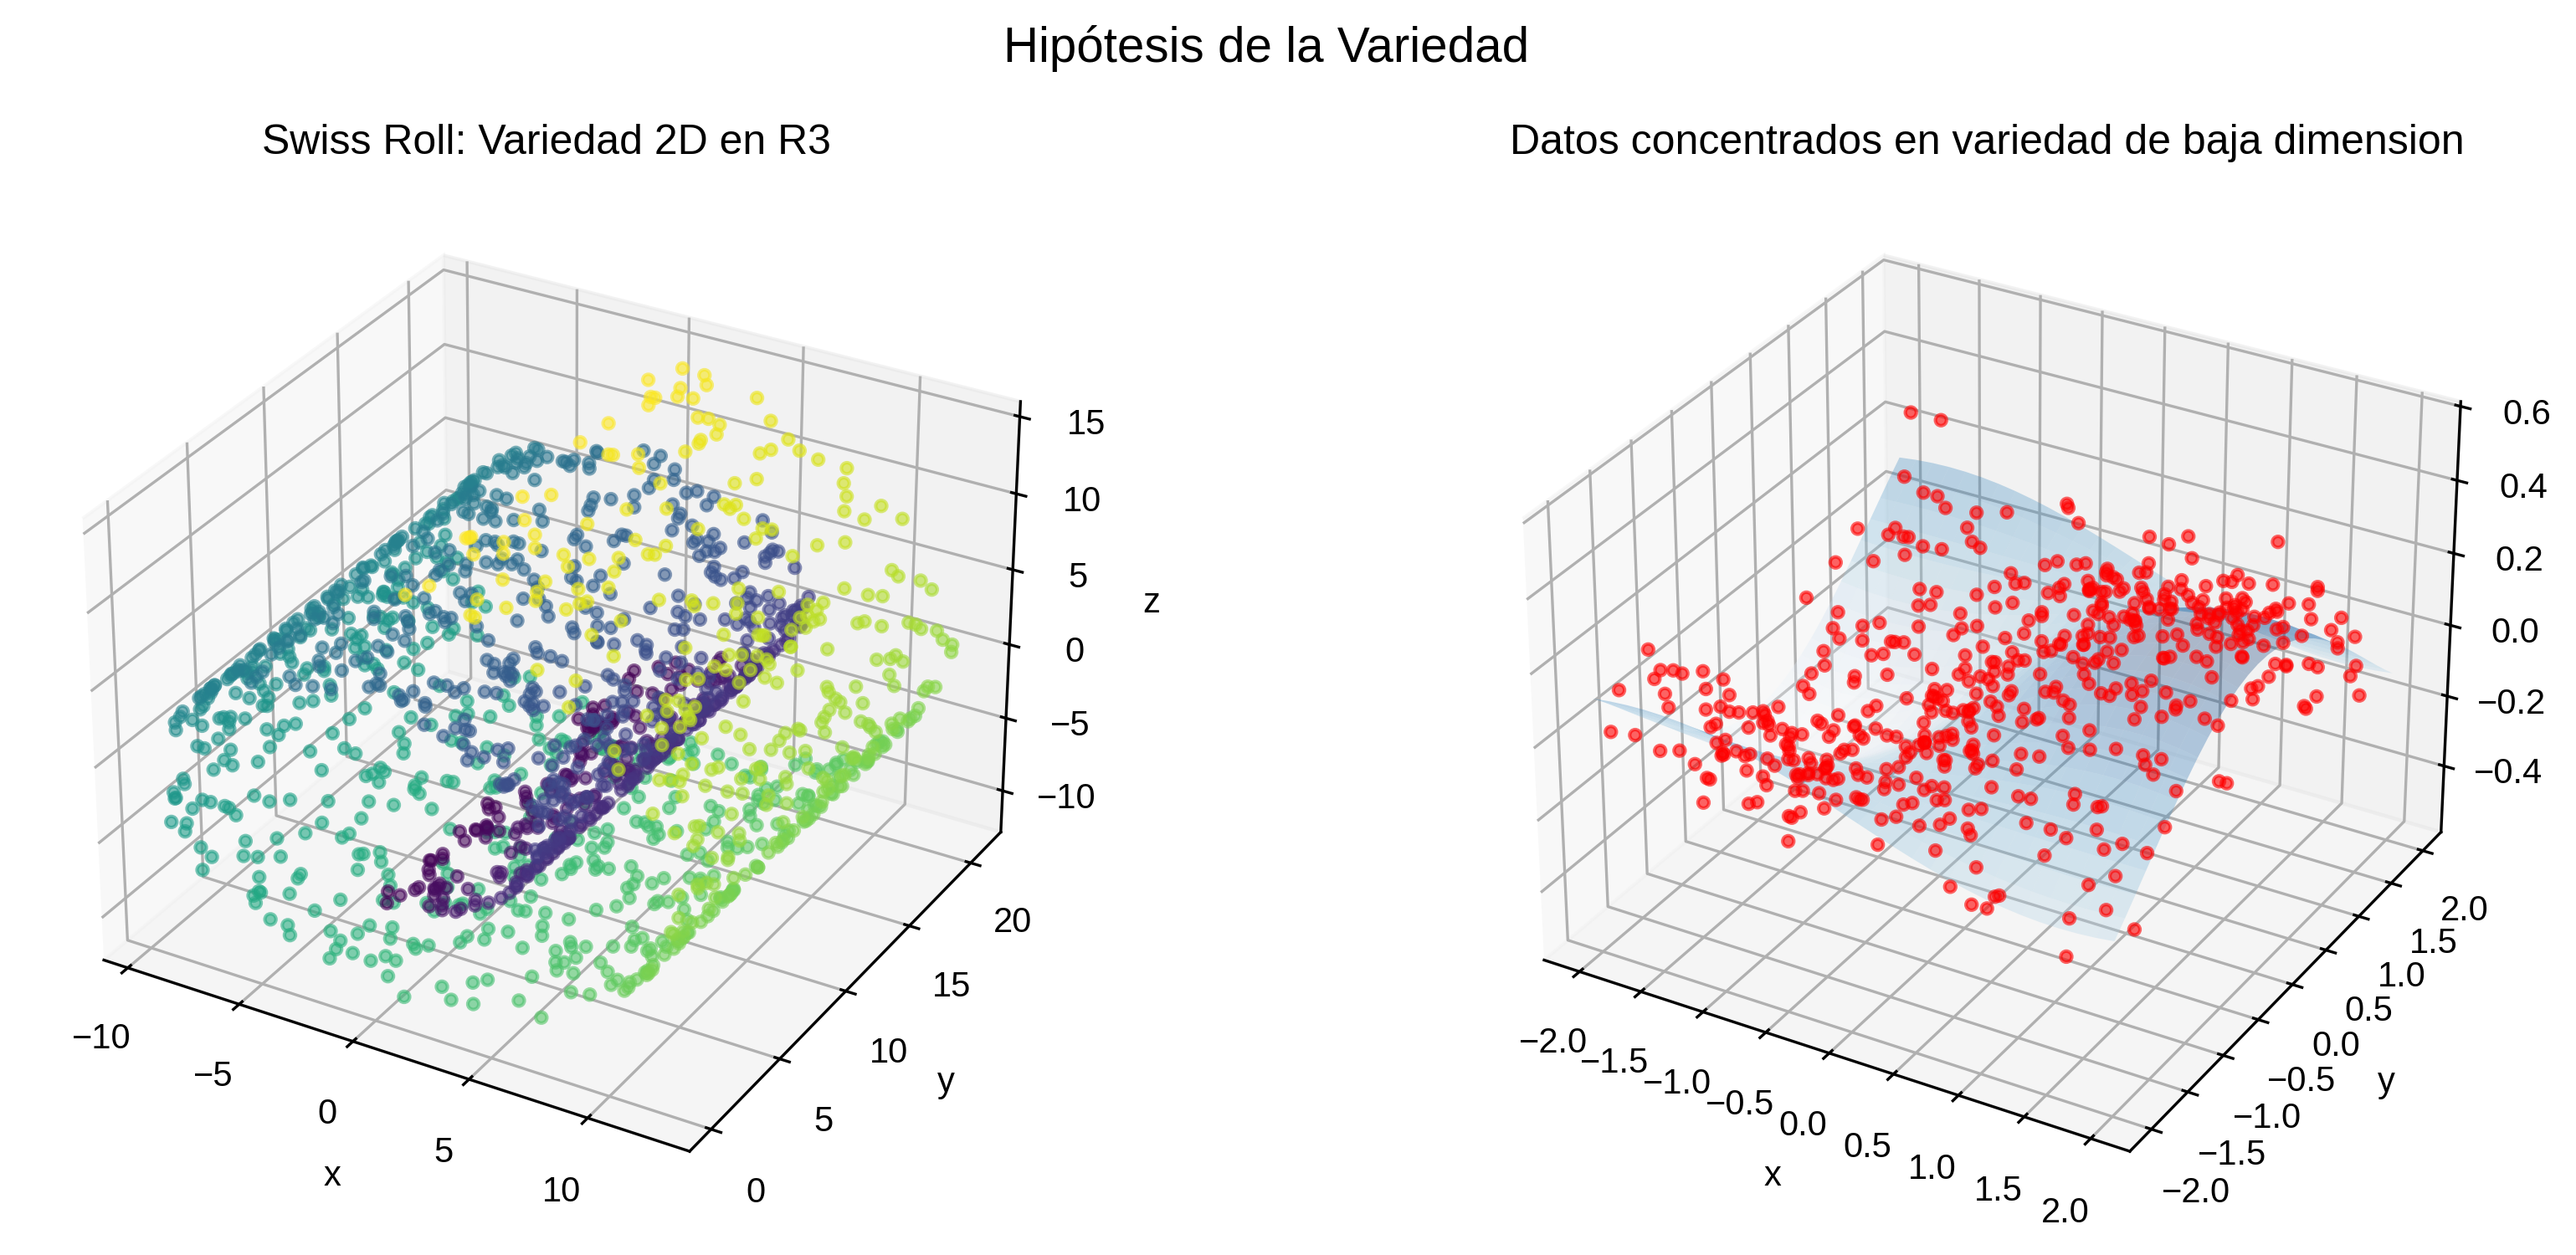
\includegraphics[width=0.9\textwidth]{images/manifold_hypothesis.png}
\caption[Hipótesis de la variedad]{Ilustración de la hipótesis de la variedad. Izquierda: el toro $\mathbb{T}^2$ como variedad bidimensional embebida en $\mathbb{R}^3$. Derecha: paraboloide hiperbólico (silla de montar) con datos distribuidos sobre la superficie, ilustrando cómo datos de alta dimensión se concentran en variedades de baja dimensión.}
\label{fig:manifold_hypothesis}
\end{figure}

\begin{hypothesis}[Hipótesis de la variedad]\label{hyp:hipotesis_variedad_gdl}
Los datos de alta dimensión en aplicaciones reales típicamente yacen cerca de una variedad $\mathcal{M}$ de dimensión intrínseca $m \ll d$ inmersa en $\mathbb{R}^d$. Formalmente, existe una variedad diferenciable $\mathcal{M}$ tal que la densidad de probabilidad de los datos $p(\mathbf{x})$ se concentra en un entorno de $\mathcal{M}$:
\[
p(\mathbf{x}) \approx 0 \quad \text{para } \mathbf{x} \notin \mathcal{U}_\epsilon(\mathcal{M})
\]
donde $\mathcal{U}_\epsilon(\mathcal{M})$ es un entorno $\epsilon$-tubular de $\mathcal{M}$.
\end{hypothesis}

Esta hipótesis no es meramente especulativa: tiene fundamento teórico sólido y evidencia empírica abundante. Los siguientes fundamentales caracterizan la estructura de variedades en espacios de alta dimensión.

\begin{theorem}[Teorema de Inmersión de Whitney]\label{thm:whitney_embedding}
Sea $\mathcal{M}$ una variedad diferenciable compacta de dimensión $m$. Entonces $\mathcal{M}$ puede ser embebida de forma suave en $\mathbb{R}^{2m+1}$ y, si $m > 1$, sumergida en $\mathbb{R}^{2m-1}$.
\end{theorem}

\begin{proof}[Esbozo]
La demostración procede en dos fases: primero se construye un embebimiento en un espacio euclidiano de dimensión arbitrariamente grande, y luego se reduce iterativamente la dimensión hasta alcanzar $\mathbb{R}^{2m+1}$.

\textbf{Paso 1: Inmersión en dimensión alta.}
Por compacidad, $\mathcal{M}$ admite un atlas finito $\{(U_i, \phi_i)\}_{i=1}^N$. Sea $\{\rho_i\}_{i=1}^N$ una partición de la unidad subordinada a este recubrimiento, es decir, funciones suaves $\rho_i: \mathcal{M} \to [0,1]$ con $\operatorname{supp}(\rho_i) \subset U_i$ y $\sum_i \rho_i \equiv 1$. Definimos $F: \mathcal{M} \to \mathbb{R}^{N(m+1)}$ por:
\[
F(p) = \bigl(\rho_1(p)\phi_1(p), \ldots, \rho_N(p)\phi_N(p), \rho_1(p), \ldots, \rho_N(p)\bigr)
\]
donde $\rho_i(p)\phi_i(p) = 0$ cuando $p \notin U_i$.

\textbf{Paso 2: $F$ es un embebimiento.}
La aplicación $F$ es suave por ser composición de funciones suaves. Es inyectiva: si $F(p) = F(q)$, las últimas $N$ componentes dan $\rho_i(p) = \rho_i(q)$ para todo $i$; eligiendo $i$ con $\rho_i(p) > 0$, las primeras componentes dan $\rho_i(p)\phi_i(p) = \rho_i(q)\phi_i(q)$, de donde $\phi_i(p) = \phi_i(q)$ y por tanto $p = q$. Para ver que $dF_p$ (\autoref{def:diferencial_aplicacion_suave}) es inyectiva, fijamos $i$ con $\rho_i(p) > 0$: el bloque correspondiente del diferencial contiene $\rho_i(p) \cdot d(\phi_i)_p$, que tiene rango $m$ por ser $\phi_i$ un difeomorfismo local. Como $\mathcal{M}$ es compacta, por la \autoref{rem:compacta_inmersion_embebimiento} esta inmersión inyectiva es un embebimiento.

\textbf{Paso 3: Reducción de dimensión.}
Se proyecta iterativamente de $\mathbb{R}^k$ a $\mathbb{R}^{k-1}$ eligiendo una dirección $\mathbf{v} \in S^{k-1}$ y proyectando ortogonalmente sobre $\mathbf{v}^\perp \cong \mathbb{R}^{k-1}$. La proyección $\pi_\mathbf{v}$ restringida a $F(\mathcal{M})$ falla en ser embebimiento solo si $\mathbf{v}$ es tangente a $F(\mathcal{M})$ (pérdida de inyectividad del diferencial) o si $\mathbf{v}$ es una dirección secante, es decir, $\mathbf{v} \propto F(p) - F(q)$ para algún par $p \neq q$ (pérdida de inyectividad global). El conjunto de direcciones tangentes tiene dimensión $\leq 2m - 1$ en $S^{k-1}$ (imagen del fibrado tangente unitario, de dimensión $2m-1$) y el de direcciones secantes tiene dimensión $\leq 2m$ (imagen de $\mathcal{M} \times \mathcal{M} \setminus \Delta$, de dimensión $2m$). Por el Teorema de Sard (\autoref{thm:sard}, véase la \autoref{sec:sard} del Apéndice~\ref{ch:teoremas_complementarios}), el conjunto de valores críticos de las aplicaciones que parametrizan estas direcciones tiene medida nula en $S^{k-1}$. Como $\dim S^{k-1} = k - 1 > 2m$ cuando $k > 2m + 1$, existen direcciones ``buenas'' y la proyección preserva el embebimiento. Iterando, se obtiene un embebimiento en $\mathbb{R}^{2m+1}$.

\textbf{Versión fuerte.}
La mejora de $\mathbb{R}^{2m+1}$ a $\mathbb{R}^{2m}$ requiere técnicas adicionales (el ``truco de Whitney'') para eliminar auto-intersecciones residuales; véase \citep[Capítulo 6]{lee2012introduction}.
\end{proof}

El teorema de Whitney garantiza que cualquier variedad compacta $m$-dimensional puede representarse fielmente en $\mathbb{R}^{2m+1}$. Esto justifica teóricamente por qué las representaciones de alta dimensión funcionan: si los datos realmente residen en una variedad de dimensión $m$, entonces embeddings en $\mathbb{R}^{2m+1}$ o más son suficientes para capturar toda su estructura geométrica. Sin embargo, el teorema no proporciona un algoritmo constructivo eficiente, lo cual motiva el uso de técnicas de reducción de dimensionalidad como autoencoders variacionales y \gls{GDL}.

\begin{definition}[Reach de una variedad]\label{def:reach}
Sea $\mathcal{M} \subset \mathbb{R}^d$ una variedad cerrada embebida. El \textit{reach} de $\mathcal{M}$, denotado $\tau(\mathcal{M})$, es el valor máximo de $r > 0$ tal que cualquier punto $\mathbf{x} \in \mathbb{R}^d$ con $d(\mathbf{x}, \mathcal{M}) < r$ tiene una proyección única sobre $\mathcal{M}$.
\end{definition}

El reach caracteriza cuán ``regular'' es la geometría de la variedad: reach grande indica curvatura suave y ausencia de auto-proximidad, mientras que reach pequeño indica geometría compleja con regiones de alta curvatura.

\begin{proposition}[Complejidad muestral en variedades]\label{prop:complejidad_muestral_variedades}
Sea $\mathcal{M}$ una variedad riemanniana compacta (\autoref{def:espacio_compacto}) de dimensión $m$, con reach $\tau > 0$ y curvatura seccional acotada en valor absoluto por $\kappa$. Entonces, para aproximar uniformemente una función $L$-Lipschitz $f: \mathcal{M} \to \mathbb{R}$ con error $\epsilon$ a partir de muestras, se requieren
\[
N = \Omega\left(\left(\frac{1}{\epsilon}\right)^m \cdot \operatorname{poly}(\tau^{-1}, \kappa)\right)
\]
muestras \citep{niyogi2008finding}.
\end{proposition}

Para un esbozo de la demostración basado en números de recubrimiento y comparación de volúmenes, véase la \autoref{sec:complejidad_muestral} del Apéndice~\ref{ch:teoremas_complementarios}.

Esta proposición revela que la complejidad muestral depende de la \textbf{dimensión intrínseca} $m$ de la variedad, no de la dimensión ambiente $d$. Este es el ``blessing of dimensionality'': si los datos de alta dimensión realmente residen en una variedad de baja dimensión, entonces el número de muestras necesarias para el aprendizaje es exponencialmente menor que lo que sugeriría la dimensión ambiente. Esto explica por qué las redes neuronales funcionan efectivamente en espacios de alta dimensión como imágenes ($d \sim 10^6$) o secuencias de texto ($d \sim 10^4$): la dimensión intrínseca efectiva $m$ es mucho menor.

\paragraph{Ejemplos de variedades en datos reales}

La hipótesis de la variedad no es abstracta: se manifiesta concretamente en dominios de aplicación reales:

\begin{itemize}
    \item \textbf{Imágenes naturales}: Aunque una imagen de $256 \times 256$ RGB es formalmente un vector en $\mathbb{R}^{196608}$, las imágenes naturales no llenan uniformemente este espacio. Se concentran en una variedad de dimensión estimada entre 10 y 100, determinada por estructuras semánticas (objetos, texturas, iluminación) y estadísticas naturales.

    \item \textbf{Configuraciones de robots articulados}: Un brazo robótico con $n$ articulaciones tiene configuraciones que residen en el producto de círculos $(S^1)^n$, una variedad compacta de dimensión $n$. Aunque podemos representar cada configuración como un vector de ángulos en $\mathbb{R}^n$, la topología intrínseca es no-euclidiana: el ángulo $2\pi$ es idéntico al ángulo $0$.

    \item \textbf{Datos de difusión MRI cerebral}: Las fibras neuronales en imágenes de difusión por resonancia magnética viven en el fibrado tangente de la variedad cerebral. En cada vóxel, la dirección de difusión es un vector tangente a la superficie cortical, no un vector arbitrario en $\mathbb{R}^3$.
\end{itemize}

\subsection{Espacios No-Euclidianos}\label{subsec:espacios_no_euclidianos}

La hipótesis de la variedad establece que los datos residen en variedades de baja dimensión, pero estas variedades son, en general, espacios no euclidianos cuya geometría intrínseca difiere de la euclidiana. Los espacios no-euclidianos proporcionan, por tanto, el marco geométrico concreto para modelar las variedades de datos: cada tipo de curvatura y topología da lugar a operaciones geométricas distintas que, como veremos, determinan la arquitectura neuronal apropiada. Notablemente, todas las geometrías que estudiaremos en esta sección (esferas, espacios proyectivos, variedades de Grassmann, espacios hiperbólicos) comparten una estructura algebraica común que permite construir arquitecturas equivariantes de forma unificada; esta estructura se formaliza en la \autoref{subsec:espacios_homogeneos}.

\paragraph{Origen de las geometrías no euclidianas}

Las geometrías no euclidianas surgen de modificar el quinto postulado de Euclides. En el lenguaje de la geometría diferencial moderna (\autoref{subsec:variedades_riemannianas}), esta modificación corresponde a considerar variedades riemannianas con curvatura no nula:

\begin{itemize}
    \item \textbf{Geometría hiperbólica} \citep{gray2007worlds}: Por un punto exterior a una recta pasan \textit{infinitas} rectas paralelas. Desarrollada independientemente por Lobachevsky y Bolyai hacia 1830, corresponde a variedades con curvatura seccional constante $K < 0$. El modelo canónico es el espacio hiperbólico $\mathbb{H}^n$ con $K = -1$.
    \item \textbf{Geometría elíptica/esférica} \citep{riemann1854hypothesen}: Por un punto exterior a una recta no pasa \textit{ninguna} recta paralela (todas las geodésicas se intersectan). Formalizada por Riemann en 1854, corresponde a variedades con curvatura seccional constante $K > 0$. El modelo canónico es la esfera $S^n$ con $K = +1$.
\end{itemize}

En el contexto del \gls{GDL}, estas propiedades geométricas (véase \autoref{rem:significado_curvatura}) tienen implicaciones directas para el diseño de arquitecturas neuronales: la curvatura del dominio determina cómo se propaga la información entre puntos vecinos, pues en espacios de curvatura positiva la información converge (facilitando agregación global), mientras que en curvatura negativa la capacidad representacional crece exponencialmente con la distancia (facilitando representaciones jerárquicas). Elegir el espacio geométrico adecuado equivale, en este sentido, a incorporar un sesgo inductivo geométrico en la arquitectura. Examinamos a continuación cada espacio concreto, presentando su definición formal, sus propiedades geométricas y sus aplicaciones características.


\begin{figure}[htbp]
\centering
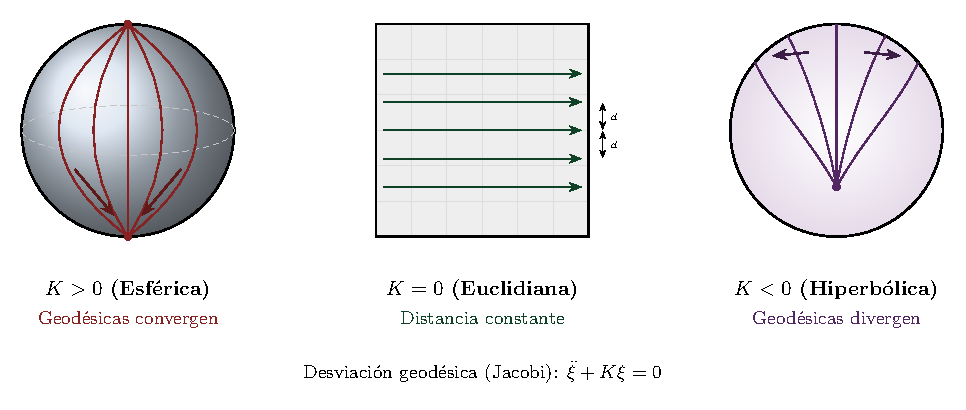
\includegraphics[width=0.85\textwidth]{images/curvature_comparison.pdf}
\caption[Comparación de geometrías según la curvatura]{Comparación de las tres geometrías clásicas según el signo de la curvatura seccional $K$. En curvatura positiva ($K > 0$), las geodésicas convergen, facilitando la agregación global de información. En curvatura nula ($K = 0$), las geodésicas mantienen distancia constante (geometría euclidiana). En curvatura negativa ($K < 0$), las geodésicas divergen exponencialmente, proporcionando mayor capacidad representacional para datos jerárquicos.}
\label{fig:curvature_comparison}
\end{figure}

\paragraph{Esferas y espacios proyectivos: datos direccionales}

\begin{definition}[Esfera $n$-dimensional]\label{def:esfera_n}
La \textit{esfera $n$-dimensional} es la variedad:
\[
S^n = \{x \in \mathbb{R}^{n+1} : \|x\| = 1\}
\]
La métrica riemanniana inducida por la métrica euclidiana ambiente tiene curvatura seccional constante $+1$ (véase el \autoref{thm:curvatura_esfera} del Apéndice~\ref{ch:teoremas_complementarios}).
\end{definition}

Las esferas $S^{n-1} \subset \mathbb{R}^n$ son fundamentales para datos direccionales donde solo la orientación importa, no la magnitud, con métrica intrínseca dada por la distancia angular:
\[
d_{S^{n-1}}(\mathbf{u}, \mathbf{v}) = \arccos(\mathbf{u}^T \mathbf{v})
\]

\textbf{Aplicaciones clave}:
\begin{itemize}
    \item \textbf{Visión omnidireccional}: Imágenes panorámicas $360^\circ$ viven naturalmente en $S^2$. Las \glspl{SphericalCNN} \citep{cohen2018sphericalcnns} operan directamente sobre la esfera usando convoluciones equivariantes bajo $SO(3)$, evitando las distorsiones de proyecciones planas (véase \autoref{subsec:spherical_cnns_so3}).

    \item \textbf{Embeddings normalizados}: En aprendizaje métrico, normalizar embeddings a la esfera unitaria $S^{d-1}$ mejora la capacidad de generalización al enfocarse en direccionalidad en lugar de magnitud \citep{wang2017normface} (véase \autoref{subsec:atencion_esfera}).

    \item \textbf{Orientaciones moleculares}: Direcciones de enlaces químicos y momentos dipolares son naturalmente elementos de $S^2$, con simetrías rotacionales bajo $SO(3)$.

    \item \textbf{Implicación arquitectónica}: La curvatura positiva constante de $S^n$ implica que las convoluciones deben reemplazar las traslaciones euclidianas por rotaciones del grupo $SO(n+1)$. Las \glspl{SphericalCNN} explotan esto definiendo la convolución como correlación cruzada sobre $SO(3)$, garantizando equivarianza rotacional exacta en lugar de aproximada (véase \autoref{subsec:spherical_cnns_so3}).
\end{itemize}

En muchas aplicaciones, los datos representan \textit{direcciones} pero no distinguen entre sentidos opuestos: una línea en una imagen, un eje de rotación, o una dirección principal en \gls{PCA}. Estos datos no viven en la esfera $S^{n-1}$ (donde $\mathbf{v}$ y $-\mathbf{v}$ son puntos distintos), sino en el \textbf{espacio proyectivo real}.

\begin{definition}[Espacio Proyectivo Real]\label{def:espacio_proyectivo}
El \textit{espacio proyectivo real} $\mathbb{RP}^n$ es el espacio de líneas que pasan por el origen en $\mathbb{R}^{n+1}$, es decir, el cociente de $S^n$ por la identificación antipodal $x \sim -x$:
\[
\mathbb{RP}^n = S^n / \{\pm 1\}
\]
Como variedad, $\dim \mathbb{RP}^n = n$, pues la proyección antipodal $\pi: S^n \to \mathbb{RP}^n$ es un recubrimiento doble (difeomorfismo local). El espacio $\mathbb{RP}^n$ es compacto y conexo (imagen continua de $S^n$), pero no simplemente conexo: su grupo fundamental es $\pi_1(\mathbb{RP}^n) \cong \mathbb{Z}/2\mathbb{Z}$, siendo $S^n$ ($n \geq 2$) su recubrimiento universal.

Casos concretos: $\mathbb{RP}^1 \cong S^1$ (el círculo, pues la identificación de puntos diametralmente opuestos en $S^1$ produce nuevamente un círculo); $\mathbb{RP}^2$ es la primera variedad cerrada no orientable (la banda de Möbius es un subconjunto abierto de $\mathbb{RP}^2$).
\end{definition}

La métrica canónica de $\mathbb{RP}^n$ se hereda de la métrica redonda de $S^n$ mediante la proyección antipodal, que es una isometría local (recubrimiento riemanniano):
\[
d_{\mathbb{RP}^n}([x], [y]) = \arccos(|x^T y|)
\]
El valor absoluto en el argumento del arcoseno distingue esta métrica de la esférica $d_{S^n}(x,y) = \arccos(x^T y)$, reflejando que $[x] = [-x]$ en $\mathbb{RP}^n$. Como $\pi: S^n \to \mathbb{RP}^n$ es un recubrimiento riemanniano (isometría local), la curvatura seccional de $\mathbb{RP}^n$ es constante $+1$, igual que la de $S^n$; las diferencias geométricas entre ambos espacios son puramente globales (orientabilidad, grupo fundamental).

\textbf{Aplicaciones clave} de los espacios proyectivos:
\begin{itemize}
    \item \textbf{Visión por computador}: Líneas y bordes en imágenes son elementos de $\mathbb{RP}^2$, ya que una línea no tiene ``dirección preferida''. Las redes que procesan estos datos deben ser invariantes bajo la identificación antipodal $\mathbf{v} \sim -\mathbf{v}$; el álgebra geométrica proyectiva proporciona un marco natural para codificar esta simetría \citep{dehaan2024euclideanprojectiveconformalchoosing}.

    \item \textbf{Análisis de componentes principales}: Los ejes principales de \gls{PCA} son direcciones sin signo, elementos de $\mathbb{RP}^{n-1}$. Los métodos de optimización sobre $\mathbb{RP}^{n-1}$ requieren gradientes riemannianos en lugar de euclidianos, pues la identificación antipodal convierte al espacio en una variedad no trivial.

    \item \textbf{Implicación arquitectónica}: La estructura de cociente $\mathbb{RP}^{n-1} = S^{n-1}/\mathbb{Z}_2$ implica que las capas neuronales deben ser equivariantes bajo la acción antipodal. Una capa proyectiva se puede construir tomando una capa esférica y simetrizando: $f([x]) = g(x) + g(-x)$. Como espacio homogéneo, $\mathbb{RP}^{n-1} \cong O(n)/(O(n-1) \times \mathbb{Z}_2)$ (\autoref{prop:proyectivo_cociente}), y esta representación guía la construcción de redes equivariantes sobre el espacio proyectivo.
\end{itemize}

\begin{definition}[Variedad de Grassmann]\label{def:variedad_grassmann}
La \textit{variedad de Grassmann} $Gr(k,n)$ es el espacio de todos los subespacios $k$-dimensionales de $\mathbb{R}^n$. Es una variedad compacta de dimensión $\dim Gr(k,n) = k(n-k)$. Cada punto de $Gr(k,n)$ se puede representar de forma única mediante la matriz de proyección ortogonal $P \in \mathbb{R}^{n \times n}$ sobre el subespacio correspondiente, caracterizada por:
\[
P^2 = P, \qquad P^T = P, \qquad \operatorname{tr}(P) = k
\]
El espacio proyectivo real es el caso especial $\mathbb{RP}^{n-1} = Gr(1,n)$ (líneas por el origen). Como casos concretos: $Gr(1,3) = \mathbb{RP}^2$ parametriza las líneas en $\mathbb{R}^3$, y $Gr(2,4)$ (planos en $\mathbb{R}^4$) tiene dimensión $2 \cdot 2 = 4$.
\end{definition}

La métrica natural de $Gr(k,n)$ se basa en los \textit{ángulos principales} entre subespacios. Dados $U, V \in Gr(k,n)$, los ángulos principales $\theta_1, \ldots, \theta_k \in [0, \pi/2]$ son los ángulos entre los pares de vectores más alineados de $U$ y $V$ (definidos recursivamente como $\cos \theta_i = \max_{u \in U, v \in V} u^T v$ sujeto a ortonormalidad con los pares anteriores). La distancia geodésica es:
\[
d_{Gr}(U, V) = \sqrt{\sum_{i=1}^{k} \theta_i^2}
\]
Cuando $k = 1$, esta métrica se reduce a la de Fubini-Study sobre $\mathbb{RP}^{n-1}$. La variedad de Grassmann posee además una simetría natural $Gr(k,n) \cong Gr(n-k,n)$ (dualidad por complemento ortogonal: a cada subespacio $V$ le corresponde $V^\perp$), que en dimensión $k(n-k) = (n-k)k$ se refleja en la igualdad de dimensiones.

Las variedades de Grassmann son relevantes para datos que representan subespacios lineales en lugar de puntos. Dado que los subespacios no admiten suma ni escalado estándar, las operaciones de red neuronal deben respetar la geometría curva de $Gr(k,n)$.

\textbf{Aplicaciones clave}:
\begin{itemize}
    \item \textbf{Reconocimiento de acciones en video}: Secuencias de fotogramas se modelan como subespacios de $\mathbb{R}^n$, y la clasificación opera sobre $Gr(k,n)$ con métricas geodésicas entre subespacios. Las GrassmannNet de \citet{huang2017grassmann} definen capas que operan mediante proyecciones y re-ortogonalizaciones que preservan la estructura de subespacio.

    \item \textbf{Análisis de componentes principales local}: En muchas tareas de visión, los descriptores locales de una imagen generan subespacios cuya comparación requiere la métrica de Grassmann, no la euclidiana. La distancia geodésica basada en ángulos principales proporciona una medida de similitud intrínseca al espacio de subespacios.

    \item \textbf{Implicación arquitectónica}: Las operaciones estándar (suma, escalado) no preservan la estructura de subespacio en $Gr(k,n)$, por lo que las redes neuronales deben redefinir sus operaciones básicas: la propagación utiliza mapas exponenciales y logarítmicos entre el espacio tangente y la variedad, y las capas lineales se reemplazan por transformaciones que preservan la pertenencia a $Gr(k,n)$ \citep{huang2017grassmann}. Como espacio homogéneo, $Gr(k,n) \cong O(n)/(O(k) \times O(n-k))$ (\autoref{prop:grassmann_stiefel_cociente}), lo que permite derivar las operaciones de red a partir de la teoría de representaciones del grupo ortogonal.
\end{itemize}


\paragraph{Espacios hiperbólicos: datos jerárquicos}

\begin{definition}[Espacio Hiperbólico]\label{def:espacio_hiperbolico}
El \textit{espacio hiperbólico} $\mathbb{H}^n$ es el único espacio de curvatura seccional constante $-1$ que es simplemente conexo (la demostración de que $K = -1$ se presenta en el \autoref{thm:curvatura_hiperbolico} del Apéndice~\ref{ch:teoremas_complementarios}). Geométricamente, es el análogo $n$-dimensional del plano hiperbólico de Lobachevsky-Bolyai.
\end{definition}

\textbf{Modelos del espacio hiperbólico.}\label{rem:modelos_hiperbolico} Existen varios modelos isométricos de $\mathbb{H}^n$:
\begin{itemize}
    \item \textbf{Modelo del disco de Poincaré}: $\mathbb{D}^n = \{x \in \mathbb{R}^n : \|x\| < 1\}$
          con métrica $ds^2 = \frac{4}{(1 - \|\mathbf{x}\|^2)^2} \sum_{i=1}^n (dx^i)^2$
    \item \textbf{Modelo del semiplano superior}: $\mathbb{H}^2 = \{z \in \mathbb{C} : \Im(z) > 0\}$
          con métrica $ds^2 = \frac{dx^2 + dy^2}{y^2}$
    \item \textbf{Modelo del hiperboloide}: Superficie $x_0^2 - x_1^2 - \cdots - x_n^2 = 1$ en $\mathbb{R}^{n+1}$
\end{itemize}

Estos tres modelos son isométricos como variedades riemannianas; la demostración explícita de las isometrías entre ellos (mediante proyección estereográfica y la transformada de Cayley) se presenta en la \autoref{sec:isometrias_hiperbolico} del Apéndice~\ref{ch:teoremas_complementarios}.

Los espacios hiperbólicos $\mathbb{H}^n$ poseen curvatura negativa constante, lo que les confiere una propiedad geométrica distintiva: el volumen de bolas geodésicas crece exponencialmente con el radio. Esta característica los hace ideales para representar datos jerárquicos y con estructura de árbol.

\textbf{Aplicaciones clave}:
\begin{itemize}
    \item \textbf{Grafos de conocimiento y semántica léxica}: Las jerarquías taxonómicas (WordNet, ontologías biológicas) y las relaciones de hiperonimia (is-a) en lenguaje natural se embeben con menor distorsión en $\mathbb{H}^n$ que en $\mathbb{R}^n$ \citep{nickel2017poincare}. La dimensionalidad requerida es logarítmica en lugar de exponencial (véase la Sección~\ref{subsubsec:embeddings_hiperbolicos_grafos} para la justificación matemática y su conexión con mecanismos de atención hiperbólica).

    \item \textbf{Redes sociales}: Comunidades jerárquicas en redes sociales exhiben estructura de árbol que se captura naturalmente en geometría hiperbólica \citep{krioukov2010hyperbolic}.
\end{itemize}

\textbf{Implicación arquitectónica}: La curvatura negativa de $\mathbb{H}^n$ exige redefinir las operaciones básicas de redes neuronales. La suma de vectores se reemplaza por la \textit{adición de Möbius} en el modelo del disco de Poincaré, y la multiplicación matricial se adapta mediante \textit{mapas exponenciales y logarítmicos} que transportan vectores entre el espacio tangente (euclidiano) y la variedad (hiperbólica). El modelo del disco de Poincaré $\mathbb{D}^n$ es el más utilizado computacionalmente por su diferenciabilidad y compatibilidad con optimización por gradiente \citep{nickel2017poincare}.

\begin{figure}[htbp]
\centering
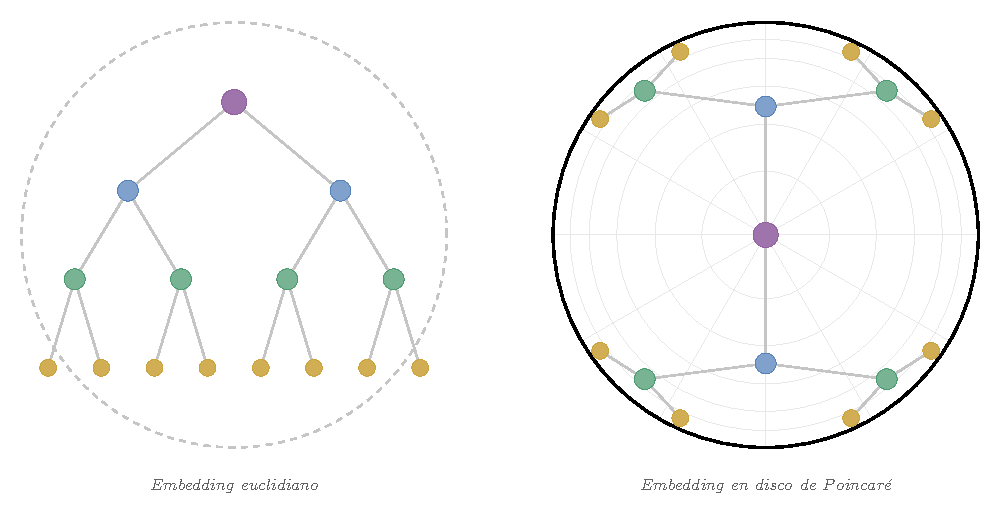
\includegraphics[width=\textwidth]{images/hyperbolic_embedding}
\caption[Embedding jerárquico en el disco de Poincaré]{Embedding de una estructura jerárquica en el disco de Poincaré $\mathbb{D}^2$. El crecimiento exponencial del volumen en geometría hiperbólica permite representar árboles y jerarquías con distorsión mínima, en contraste con el espacio euclidiano donde la dimensionalidad requerida crece exponencialmente.}
\label{fig:hyperbolic_embedding}
\end{figure}

\paragraph{Espacios producto y compuestos: datos multiestructurados}

Muchos datos reales combinan múltiples tipos de geometría. Los \textbf{espacios producto} permiten modelar esta heterogeneidad estructural.

\begin{definition}[Variedad Producto]\label{def:variedad_producto}
Dadas dos variedades riemannianas $(\mathcal{M}, g_\mathcal{M})$ y $(\mathcal{N}, g_\mathcal{N})$, la \textit{variedad producto} $\mathcal{M} \times \mathcal{N}$ es la variedad cuyo conjunto subyacente es el producto cartesiano, equipada con la \textit{métrica producto}:
\[
g_{(p,q)}((v_1, w_1), (v_2, w_2)) = g_{\mathcal{M},p}(v_1, v_2) + g_{\mathcal{N},q}(w_1, w_2)
\]
para $p \in \mathcal{M}$, $q \in \mathcal{N}$, $v_i \in T_p\mathcal{M}$, $w_i \in T_q\mathcal{N}$.
\end{definition}

\begin{proposition}[Propiedades de variedades producto]\label{prop:propiedades_producto}
La variedad producto $\mathcal{M} \times \mathcal{N}$ satisface:
\begin{enumerate}
    \item $\dim(\mathcal{M} \times \mathcal{N}) = \dim \mathcal{M} + \dim \mathcal{N}$
    \item Las geodésicas son productos de geodésicas: $\gamma(t) = (\gamma_\mathcal{M}(t), \gamma_\mathcal{N}(t))$
    \item Las curvaturas seccionales de planos tangentes a cada factor se preservan
\end{enumerate}
\end{proposition}

\begin{proof}
\leavevmode
\begin{enumerate}
    \item \textbf{Dimensión.} Los espacios tangentes satisfacen $T_{(p,q)}(\mathcal{M} \times \mathcal{N}) \cong T_p\mathcal{M} \oplus T_q\mathcal{N}$, luego $\dim(\mathcal{M} \times \mathcal{N}) = \dim T_p\mathcal{M} + \dim T_q\mathcal{N} = \dim \mathcal{M} + \dim \mathcal{N}$.

    \item \textbf{Geodésicas.} La métrica producto $g = g_\mathcal{M} + g_\mathcal{N}$ tiene estructura bloque-diagonal en los espacios tangentes. La ecuación de geodésicas $\nabla_{\dot\gamma}\dot\gamma = 0$ se desacopla en las componentes de cada factor, pues los símbolos de Christoffel mixtos se anulan. Luego $\gamma(t) = (\gamma_\mathcal{M}(t), \gamma_\mathcal{N}(t))$ es geodésica si y solo si cada componente lo es en su factor.

    \item \textbf{Curvaturas seccionales.} Sea $\sigma$ un plano tangente a $\mathcal{M}$ en $(p,q)$, es decir, $\sigma \subset T_p\mathcal{M} \oplus \{0\}$. El tensor de Riemann de la métrica producto es bloque-diagonal (los términos mixtos se anulan), luego $K_{\mathcal{M}\times\mathcal{N}}(\sigma) = K_\mathcal{M}(\sigma)$. \qedhere
\end{enumerate}
\end{proof}

\begin{definition}[Toro $n$-dimensional]\label{def:toro_n}
El \textit{toro $n$-dimensional} es el producto de $n$ círculos:
\[
T^n = \underbrace{S^1 \times S^1 \times \cdots \times S^1}_{n \text{ veces}} = (\mathbb{R}/\mathbb{Z})^n
\]
El toro tiene curvatura cero (es plano) y admite coordenadas periódicas $(\theta_1, \ldots, \theta_n) \in [0, 2\pi)^n$.
\end{definition}

\textbf{Aplicaciones de espacios producto:}

\begin{itemize}
    \item \textbf{Toro} $T^n = (S^1)^n$: Para datos periódicos como series temporales cíclicas (patrones climáticos estacionales, ritmos circadianos) y análisis de Fourier.

    \item \textbf{Productos de variedades}: Grafos con atributos nodeales geométricos pueden modelarse como productos $G \times \mathcal{M}$, donde $G$ es la estructura discreta del grafo y $\mathcal{M}$ es el espacio de atributos continuos.

    \item \textbf{Embeddings de curvatura mixta}: Datos con estructura heterogénea (parcialmente jerárquica, parcialmente cíclica) se representan en productos $\mathbb{H}^{d_1} \times S^{d_2} \times \mathbb{R}^{d_3}$, donde cada componente captura un aspecto geométrico diferente de los datos. La dimensionalidad de cada factor se aprende automáticamente \citep{bronstein2017geometricdeeplearning}.
\end{itemize}

\paragraph{Grafos como geometría discreta}

Los grafos $G = (V, E)$ representan un caso especial de geometría \textit{discreta} no-euclidiana. Como se desarrolla extensamente en la \autoref{sec:grafos_discretizacion}, los grafos proporcionan una representación más flexible que los espacios euclidianos al capturar conectividad arbitraria sin imponer métricas rígidas.

\paragraph{Síntesis: geometría como sesgo inductivo}

La elección del espacio geométrico no es un mero detalle de representación: constituye un \textit{sesgo inductivo} fundamental que determina la arquitectura neuronal apropiada. Cada geometría impone restricciones específicas sobre las operaciones admisibles:

\begin{table}[htbp]
\centering
\small
\caption{Correspondencia entre geometrías, sesgos inductivos y operaciones en GDL.}
\label{tab:geometria_sesgo_operacion}
\begin{tabular}{@{}lll@{}}
    \toprule
    \textbf{Geometría} & \textbf{Sesgo inductivo} & \textbf{Operación GDL} \\
    \midrule
    $\mathbb{R}^n$ (euclidiana) & Simetría traslacional & Convolución estándar \\
    $S^n$ (esférica, $K>0$) & Simetría rotacional & Convolución sobre $SO(n{+}1)$ \\
    $\mathbb{H}^n$ (hiperbólica, $K<0$) & Jerarquía exponencial & Adición de Möbius, maps exp/log \\
    $Gr(k,n)$ (Grassmann) & Datos como subespacios & Métricas geodésicas en $Gr$ \\
    $\mathcal{M} \times \mathcal{N}$ (producto) & Estructura heterogénea & Operaciones por componente \\
    Grafos & Conectividad discreta & Message passing \\
    \bottomrule
\end{tabular}
\end{table}

Esta correspondencia entre geometría y arquitectura es el principio organizador central del \gls{GDL}: las simetrías del dominio geométrico determinan las restricciones de equivarianza que debe satisfacer la red neuronal. Notablemente, todos los espacios presentados en esta sección admiten una descripción unificada como espacios homogéneos $G/H$, como se formaliza y demuestra en la \autoref{subsec:espacios_homogeneos}; la interpretación geométrica de cada descomposición (cómo $G$ y $H$ determinan curvatura, compacidad y crecimiento de volumen) se detalla junto a cada proposición en la \autoref{subsec:espacios_homogeneos}. Los fundamentos algebraicos para formalizar estas simetrías se desarrollan en la \autoref{sec:grupos_simetrias}, y la tabla completa con arquitecturas específicas y referencias se presenta en la \autoref{rem:espacios_homogeneos_arquitecturas}.

\section{Grupos: Las Simetrías de los Datos}\label{sec:grupos_simetrias}

La sección anterior identificó los dominios geométricos donde residen los datos y señaló que cada dominio posee simetrías naturales: las traslaciones en $\mathbb{R}^n$, las rotaciones en $S^n$, las isometrías en $\mathbb{H}^n$. Pero, ¿qué significa exactamente que una arquitectura neuronal ``respete'' estas simetrías? La respuesta requiere un lenguaje algebraico preciso. La \textbf{teoría de grupos} proporciona este lenguaje: un grupo captura la colección de todas las transformaciones que preservan la estructura de un espacio, y la \textbf{teoría de representaciones} traduce estas simetrías abstractas en restricciones concretas sobre las funciones que la red puede aprender. A partir de estos fundamentos, formalizamos los conceptos de \textbf{equivarianza} e \textbf{invarianza} (\autoref{subsec:equivarianza_invarianza}) y mostramos que los dominios geométricos estudiados anteriormente admiten una descripción unificada como \textbf{espacios homogéneos} (\autoref{subsec:espacios_homogeneos}).

\subsection{Teoría de Grupos}\label{subsec:teoria_grupos_representaciones}

Comenzamos por los fundamentos algebraicos: la definición de grupo, subgrupos, acciones de grupo y grupos de Lie. Estas estructuras permiten modelar simetrías tanto discretas (permutaciones $S_n$) como continuas (rotaciones $SO(n)$, traslaciones $\mathbb{R}^d$). La progresión natural conduce desde los grupos hacia sus representaciones lineales, que son el mecanismo mediante el cual las simetrías actúan sobre los espacios de características de una red neuronal.

\begin{definition}[Operación Interna]\label{def:operacion_interna}
Una \textit{operación interna} (o binaria) en un conjunto $G$ es una función:
\begin{equation}
\cdot: G \times G \rightarrow G
\end{equation}
que asigna a cada par ordenado $(a,b) \in G \times G$ un único elemento $a \cdot b \in G$.
\end{definition}

\begin{definition}[Grupo]\label{def:grupo}
Un \textit{grupo} es un conjunto $G$ equipado con una operación interna $\cdot: G \times G \rightarrow G$ que satisface:
\begin{enumerate}
    \item \textbf{Asociatividad}: $(a \cdot b) \cdot c = a \cdot (b \cdot c)$ para todo $a, b, c \in G$
    \item \textbf{Elemento identidad}: Existe $e \in G$ tal que $e \cdot a = a \cdot e = a$ para todo $a \in G$
    \item \textbf{Elemento inverso}: Para cada $a \in G$, existe $a^{-1} \in G$ tal que $a \cdot a^{-1} = a^{-1} \cdot a = e$
\end{enumerate}
\end{definition}

\textbf{Grupos Abelianos.}\label{rem:grupos_abelianos} Un grupo $(G, \cdot)$ es \textbf{abeliano} (o conmutativo) si $a \cdot b = b \cdot a$ para todo $a, b \in G$. Las traslaciones en \glspl{CNN} forman grupos abelianos, donde el orden de aplicación de las traslaciones no afecta el resultado final: $(x,y) + (a,b) + (c,d) = (x,y) + (c,d) + (a,b)$.

\begin{definition}[Subgrupo]\label{def:subgrupo}
Sea $(G, \cdot)$ un grupo. Un subconjunto $H \subseteq G$ es un \textit{subgrupo} si $(H, \cdot)$ es grupo con la operación heredada. Notación: $H \leq G$.
\end{definition}

\begin{proposition}[Criterio de Subgrupo]\label{prop:criterio_subgrupo}
$H \leq G$ si y solo si:
\begin{enumerate}
    \item $e \in H$ (contiene el elemento identidad)
    \item $h_1, h_2 \in H \Rightarrow h_1 h_2 \in H$ (cerrado bajo la operación)
    \item $h \in H \Rightarrow h^{-1} \in H$ (contiene inversos)
\end{enumerate}
\end{proposition}

\begin{proof}
$(\Rightarrow)$ Si $H \leq G$, las tres condiciones son inmediatas por los axiomas de grupo.

$(\Leftarrow)$ Supongamos que $H$ satisface (1)--(3). La operación de $H$ es la heredada de $G$, que es asociativa por serlo en $G$. La condición (1) proporciona la identidad, (2) garantiza la clausura, y (3) la existencia de inversos. Luego $(H, \cdot)$ es grupo.
\end{proof}

\begin{definition}[Subgrupo Normal]\label{def:subgrupo_normal}
Un subgrupo $H \leq G$ es \textit{normal} (notación: $H \triangleleft G$) si:
\begin{equation}
gHg^{-1} = H \quad \text{para todo } g \in G
\end{equation}
Equivalentemente, $ghg^{-1} \in H$ para todo $g \in G$ y $h \in H$.
\end{definition}

\begin{definition}[Orden de un Grupo]\label{def:orden_grupo}
El \textit{orden} de un grupo $G$, denotado $|G|$, es su cardinalidad. El \textbf{índice} de un subgrupo $H \leq G$, denotado $[G:H]$, es el número de clases laterales de $H$ en $G$.
\end{definition}

Para grupos finitos, el orden del grupo y el de cualquier subgrupo están relacionados de manera precisa por el Teorema de Lagrange (\autoref{thm:lagrange}, véase \autoref{sec:lagrange} del Apéndice~\ref{ch:teoremas_complementarios}).

Los conceptos de subgrupo normal y orden de grupo nos conducen naturalmente hacia una construcción algebraica fundamental: el grupo cociente. Cuando un subgrupo $H$ es normal en $G$, las clases laterales $gH$ no solo particionan el grupo, sino que heredan una estructura de grupo bien definida. Esta construcción es esencial en \gls{GDL} porque permite modelar reducciones sistemáticas de simetrías en arquitecturas jerárquicas.

\paragraph{Grupo Cociente}

\begin{definition}[Grupo Cociente]\label{def:grupo_cociente}
Sea $G$ un grupo y $H \triangleleft G$ un subgrupo normal. El \textit{grupo cociente} (o grupo factor) $G/H$ es el conjunto de clases laterales izquierdas:
\begin{equation}
G/H = \{gH : g \in G\}
\end{equation}
equipado con la operación:
\begin{equation}
(g_1H) \cdot (g_2H) = (g_1g_2)H
\end{equation}
Esta operación está bien definida, como demuestra la siguiente proposición.
\end{definition}

\begin{proposition}[Buena definición de la operación cociente]\label{prop:cociente_bien_definido}
Sea $G$ un grupo y $H \leq G$ un subgrupo. La operación $(g_1H)(g_2H) = (g_1g_2)H$ en el conjunto de clases laterales $G/H$ está bien definida si y solo si $H \triangleleft G$.
\end{proposition}

\begin{proof}
$(\Leftarrow)$ Supongamos $H \triangleleft G$. Sean $g_1H = g_1'H$ y $g_2H = g_2'H$, es decir, existen $h_1, h_2 \in H$ tales que $g_1' = g_1h_1$ y $g_2' = g_2h_2$. Entonces:
\[
g_1'g_2' = g_1h_1g_2h_2 = g_1g_2\underbrace{(g_2^{-1}h_1g_2)}_{\in H}h_2
\]
Como $H \triangleleft G$, se tiene $g_2^{-1}h_1g_2 \in H$, luego $(g_2^{-1}h_1g_2)h_2 \in H$ y por tanto $(g_1'g_2')H = (g_1g_2)H$.

$(\Rightarrow)$ Supongamos que la operación está bien definida. Sean $g \in G$ y $h \in H$ arbitrarios. Como $h \in H$, tenemos $ghH = gH$. Entonces:
\[
(ghg^{-1})H = (ghH)(g^{-1}H) = (gH)(g^{-1}H) = (gg^{-1})H = eH = H
\]
donde la segunda igualdad usa la buena definición con los representantes $gh$ y $g$ de la misma clase $gH$. Así, $ghg^{-1} \in H$ para todo $g \in G$ y $h \in H$, lo que significa que $H \triangleleft G$.
\end{proof}

Los grupos cociente son fundamentales en \gls{GDL} porque modelan reducciones de simetría en arquitecturas jerárquicas. Por ejemplo, en redes que procesan datos 3D, podemos comenzar con simetrías $SE(3)$ completas y gradualmente reducir a $SO(3)$ o $SO(2)$ en capas superiores mediante morfismos naturales $SE(3) \rightarrow SO(3)$ cuyo kernel (traslaciones) forma un subgrupo normal.

La construcción de grupos cociente depende crucialmente de la existencia de funciones que preserven la estructura de grupo. Este concepto nos lleva directamente a los homomorfismos, funciones que respetan las operaciones algebraicas y constituyen el puente entre diferentes grupos. En \gls{GDL}, los homomorfismos traducen simetrías abstractas en transformaciones computables, proporcionando el mecanismo formal para implementar equivarianza en arquitecturas neuronales.

\paragraph{Homomorfismos}

\begin{definition}[Homomorfismo de Grupos]\label{def:homomorfismo_grupos}
Sean $(G, \cdot_G)$ y $(H, \cdot_H)$ grupos. Una función $\phi: G \rightarrow H$ es un \textit{homomorfismo} si:
\begin{equation}
\phi(g_1 \cdot_G g_2) = \phi(g_1) \cdot_H \phi(g_2) \quad \forall g_1, g_2 \in G
\end{equation}
\end{definition}

\begin{definition}[Isomorfismo de Grupos]\label{def:isomorfismo_grupos}
Sean $(G, \cdot_G)$ y $(H, \cdot_H)$ grupos. Un homomorfismo $\phi: G \rightarrow H$ es un \textit{isomorfismo} si es biyectivo. En este caso, decimos que $G$ y $H$ son \textit{isomorfos} y escribimos $G \cong H$.
\end{definition}

Dos grupos isomorfos tienen la misma estructura algebraica y sólo se diferencian por los símbolos utilizados para denotar los elementos y la operación. Los isomorfismos permiten transferir propiedades entre grupos estructuralmente idénticos, facilitando el análisis de simetrías complejas mediante grupos más simples o conocidos.

\begin{definition}[Núcleo e Imagen]\label{def:nucleo_imagen}
Sea $\phi: G \rightarrow H$ un homomorfismo de grupos. El \textit{núcleo} de $\phi$ es:
\begin{equation}
\ker(\phi) = \{g \in G : \phi(g) = e_H\}
\end{equation}
donde $e_H$ es la identidad de $H$. La \textit{imagen} de $\phi$ es:
\begin{equation}
\mathrm{Im}(\phi) = \{\phi(g) : g \in G\} \subseteq H
\end{equation}
El núcleo es siempre un subgrupo normal de $G$, es decir, $\ker(\phi) \triangleleft G$.
\end{definition}

\begin{theorem}[Primer Teorema de Isomorfismo]\label{thm:primer_isomorfismo}
Sea $\phi: G \rightarrow H$ un homomorfismo de grupos. Entonces:
\begin{equation}
G/\ker(\phi) \cong \mathrm{Im}(\phi)
\end{equation}
El isomorfismo está dado por $\bar{\phi}: G/\ker(\phi) \rightarrow \mathrm{Im}(\phi)$, $\bar{\phi}(g\ker(\phi)) = \phi(g)$.
\end{theorem}

\begin{proof}
\textbf{Paso 1: $\bar{\phi}$ está bien definida.} Si $g_1\ker(\phi) = g_2\ker(\phi)$, entonces $g_1^{-1}g_2 \in \ker(\phi)$, por lo que $\phi(g_1^{-1}g_2) = e_H$. Esto implica $\phi(g_1)^{-1}\phi(g_2) = e_H$, es decir, $\phi(g_1) = \phi(g_2)$.

\textbf{Paso 2: $\bar{\phi}$ es homomorfismo.}
\[
\bar{\phi}(g_1\ker(\phi) \cdot g_2\ker(\phi)) = \bar{\phi}((g_1g_2)\ker(\phi)) = \phi(g_1g_2) = \phi(g_1)\phi(g_2) = \bar{\phi}(g_1\ker(\phi)) \cdot \bar{\phi}(g_2\ker(\phi))
\]

\textbf{Paso 3: $\bar{\phi}$ es inyectiva.} Si $\bar{\phi}(g\ker(\phi)) = e_H$, entonces $\phi(g) = e_H$, por lo que $g \in \ker(\phi)$, y $g\ker(\phi) = \ker(\phi)$ es la identidad en $G/\ker(\phi)$.

\textbf{Paso 4: $\bar{\phi}$ es sobreyectiva sobre $\mathrm{Im}(\phi)$ por definición.}
\end{proof}

Este teorema es fundamental porque permite identificar grupos cociente con imágenes de homomorfismos, simplificando el análisis de estructuras algebraicas complejas.

\begin{definition}[Representación de Grupo]\label{def:representacion_grupo}
Sea $G$ un grupo y $V$ un espacio vectorial sobre un cuerpo $\mathbb{K}$. Una \textit{representación} de $G$ en $V$ es un homomorfismo de grupos:
\begin{equation}
\rho: G \rightarrow GL(V)
\end{equation}
donde $GL(V)$ denota el grupo de transformaciones lineales invertibles de $V$. Es decir, a cada elemento $g \in G$ se le asigna una matriz invertible $\rho(g)$ de modo que la composición en el grupo se traduce en producto matricial: $\rho(g_1 g_2) = \rho(g_1)\rho(g_2)$.
\end{definition}

Las representaciones son fundamentales en \gls{GDL} porque traducen simetrías abstractas en operaciones computables sobre espacios de características neuronales: cada simetría del dominio se convierte en una transformación lineal concreta que puede implementarse y optimizarse.

Los homomorfismos establecen relaciones entre grupos abstractos, pero para aplicar grupos a problemas concretos necesitamos que actúen sobre espacios de datos específicos. Esta necesidad nos conduce al concepto de acción de grupo, que formaliza cómo un grupo transforma elementos de un conjunto. Las acciones de grupo traducen simetrías abstractas en transformaciones explícitas sobre dominios geométricos concretos como imágenes, grafos o variedades.

\paragraph{Acción de Grupo}

\begin{definition}[Acción de Grupo]\label{def:accion_grupo}
Sea $G$ un grupo y $X$ un conjunto. Una \textit{acción de grupo} de $G$ sobre $X$ es una función:
\begin{equation}
\rho: G \times X \rightarrow X, \quad (g, x) \mapsto g \cdot x
\end{equation}
que satisface:
\begin{enumerate}
    \item \textbf{Compatibilidad}: $(g_1 g_2) \cdot x = g_1 \cdot (g_2 \cdot x)$ para todo $g_1, g_2 \in G$ y $x \in X$
    \item \textbf{Identidad}: $e \cdot x = x$ para todo $x \in X$, donde $e$ es el elemento identidad de $G$
\end{enumerate}
\end{definition}

\begin{proposition}[Acciones como Homomorfismos]\label{prop:acciones_homomorfismos}
Toda acción de grupo $\rho: G \times X \rightarrow X$ induce un homomorfismo de grupos:
\begin{equation}
\tilde{\rho}: G \rightarrow \text{Sym}(X), \quad \tilde{\rho}(g)(x) = g \cdot x
\end{equation}
donde $\text{Sym}(X)$ denota el grupo de biyecciones de $X$ consigo mismo.
\end{proposition}

\begin{proof}
Para cada $g \in G$, definimos $\tilde{\rho}(g): X \rightarrow X$ como la aplicación $x \mapsto g \cdot x$. Debemos verificar:
\begin{enumerate}
    \item \textbf{$\tilde{\rho}(g)$ es biyectiva}: Su inversa es $\tilde{\rho}(g^{-1})$, ya que $(g^{-1}) \cdot (g \cdot x) = (g^{-1}g) \cdot x = e \cdot x = x$.
    \item \textbf{$\tilde{\rho}$ preserva la operación}: Para $g_1, g_2 \in G$,
    \begin{equation}
    \tilde{\rho}(g_1 g_2)(x) = (g_1 g_2) \cdot x = g_1 \cdot (g_2 \cdot x) = \tilde{\rho}(g_1)(\tilde{\rho}(g_2)(x)) = (\tilde{\rho}(g_1) \circ \tilde{\rho}(g_2))(x)
    \end{equation}
\end{enumerate}
Por tanto, $\tilde{\rho}$ es un homomorfismo de $G$ en $\text{Sym}(X)$.
\end{proof}

Esta correspondencia es fundamental: estudiar acciones de $G$ sobre $X$ es equivalente a estudiar homomorfismos de $G$ en $\text{Sym}(X)$. En el contexto de \gls{GDL}, esto significa que las simetrías de los datos se traducen directamente en transformaciones concretas sobre el espacio de entrada.

\begin{example}[Acciones de Grupo en Deep Learning]\label{ex:acciones_grupo_dl}
\leavevmode
\begin{itemize}
    \item \textbf{Traslaciones en imágenes}: El grupo $\mathbb{Z}^2$ actúa sobre imágenes discretas mediante desplazamiento de píxeles
    \item \textbf{Rotaciones en datos 3D}: $SO(3)$ actúa sobre nubes de puntos mediante matrices de rotación
    \item \textbf{Permutaciones en grafos}: $S_n$ actúa sobre grafos de $n$ nodos reordenando los índices de los nodos
\end{itemize}
\end{example}

Antes de pasar a grupos de Lie, introducimos una construcción algebraica fundamental que utilizaremos para describir grupos de simetrías como el grupo euclidiano.

\begin{definition}[Producto Semidirecto]\label{def:producto_semidirecto}
Sean $N$ y $H$ grupos, y sea $\phi: H \to \mathrm{Aut}(N)$ un homomorfismo (donde $\mathrm{Aut}(N)$ es el grupo de automorfismos de $N$). El \textit{producto semidirecto} de $N$ por $H$ respecto a $\phi$, denotado $N \rtimes_\phi H$ (o simplemente $N \rtimes H$), es el conjunto $N \times H$ equipado con la operación:
\begin{equation}\label{eq:producto_semidirecto}
(n_1, h_1) \cdot (n_2, h_2) = (n_1 \cdot \phi(h_1)(n_2), h_1 \cdot h_2)
\end{equation}
donde $\phi(h_1)(n_2)$ denota la acción del automorfismo $\phi(h_1)$ sobre $n_2$.
\end{definition}

Intuitivamente, el producto semidirecto generaliza el producto directo $N \times H$ permitiendo que $H$ ``actúe'' sobre $N$ de forma no trivial. En el producto directo, los elementos de $N$ y $H$ conmutan; en el producto semidirecto, $H$ ``tuerce'' a $N$ mediante automorfismos.

\begin{example}[Grupo Euclidiano como Producto Semidirecto]\label{ex:grupo_euclidiano_semidirecto}
El \textit{grupo euclidiano} $E(n) = \mathbb{R}^n \rtimes O(n)$ es el producto semidirecto de las traslaciones $\mathbb{R}^n$ por las rotaciones y reflexiones $O(n)$. La acción $\phi: O(n) \to \mathrm{Aut}(\mathbb{R}^n)$ es la multiplicación matricial: $\phi(R)(t) = Rt$. Así, la operación de grupo es:
\begin{equation}
(t_1, R_1) \cdot (t_2, R_2) = (t_1 + R_1 t_2, R_1 R_2)
\end{equation}
Esta estructura refleja cómo las rotaciones ``afectan'' a las traslaciones: primero se rota, luego se traslada.
\end{example}

Hasta ahora hemos desarrollado la teoría de grupos desde una perspectiva puramente algebraica, tratando grupos como estructuras abstractas definidas por operaciones binarias. Sin embargo, las aplicaciones del \gls{GDL} requieren frecuentemente simetrías continuas: rotaciones suaves en $SO(3)$, traslaciones en $\mathbb{R}^d$, o transformaciones euclidianas en $SE(3)$. Esta transición de lo discreto a lo continuo nos lleva naturalmente hacia los grupos de Lie, donde la estructura algebraica se combina con la geometría diferencial.

\subsubsection{Grupos de Lie}

Las variedades diferenciables (véase \autoref{def:variedad_diferenciable}) constituyen la geometría natural donde operan muchas arquitecturas de \gls{GDL}, especialmente cuando tratamos con datos continuos como nubes de puntos 3D o superficies. Por ello, es fundamental considerar grupos de Lie en lugar de grupos abstractos, ya que las simetrías continuas requieren estructura diferenciable.

\begin{definition}[Grupo de Lie]\label{def:grupo_lie}
Un \textit{grupo de Lie} es un grupo $G$ que también es una variedad diferenciable, donde las operaciones de grupo:
\begin{itemize}
    \item \textbf{Multiplicación}: $\mu: G \times G \rightarrow G, \quad (g,h) \mapsto gh$
    \item \textbf{Inversión}: $\iota: G \rightarrow G, \quad g \mapsto g^{-1}$
\end{itemize}
son funciones suaves (de clase $C^\infty$).
\end{definition}

Los grupos de Lie constituyen la clase más importante de grupos en \gls{GDL}, ya que la mayoría de simetrías continuas en aplicaciones reales (rotaciones, traslaciones, transformaciones euclidianas) poseen estructura diferenciable natural.

\begin{definition}[Acción Suave]\label{def:accion_suave}
Sea $G$ un grupo de Lie y $M$ una variedad diferenciable. Una \textit{acción suave} de $G$ sobre $M$ es una acción de grupo $\rho: G \times M \rightarrow M$ que además es una aplicación diferenciable (de clase $C^\infty$).
\end{definition}

La condición de suavidad garantiza que las transformaciones del grupo preserven la estructura diferenciable de la variedad, permitiendo el uso de herramientas del cálculo diferencial como derivadas y flujos. En \gls{GDL}, esto es esencial para definir gradientes y realizar optimización sobre espacios de transformaciones.

\begin{definition}[Corchete de Lie]\label{def:corchete_lie}
Sea $\mathfrak{g}$ un espacio vectorial. Un \textit{corchete de Lie} es una operación binaria $[\cdot, \cdot]: \mathfrak{g} \times \mathfrak{g} \rightarrow \mathfrak{g}$ que satisface:
\begin{enumerate}
    \item \textbf{Bilinealidad}: $[aX + bY, Z] = a[X,Z] + b[Y,Z]$ para todo $a, b \in \mathbb{R}$
    \item \textbf{Antisimetría}: $[X,Y] = -[Y,X]$
    \item \textbf{Identidad de Jacobi}: $[X,[Y,Z]] + [Y,[Z,X]] + [Z,[X,Y]] = 0$
\end{enumerate}
\end{definition}

\begin{definition}[Álgebra de Lie]\label{def:algebra_lie}
Un \textit{álgebra de Lie} es un espacio vectorial $\mathfrak{g}$ equipado con un corchete de Lie $[\cdot, \cdot]: \mathfrak{g} \times \mathfrak{g} \to \mathfrak{g}$.
\end{definition}

Todo grupo de Lie $G$ lleva asociada un álgebra de Lie canónica: el espacio tangente en la identidad $T_e G$, con el corchete inducido por los campos vectoriales invariantes por la izquierda. La ventaja de esta construcción es que permite trabajar en un espacio vectorial lineal en lugar de una variedad curva, lo cual es fundamental para optimización y diferenciación en arquitecturas neuronales. El puente entre el grupo (no lineal) y su álgebra (lineal) es el \textit{mapa exponencial}.

\begin{definition}[Mapa Exponencial]\label{def:mapa_exponencial}
Sea $G$ un grupo de Lie con álgebra de Lie $\mathfrak{g}$. El \textit{mapa exponencial} es la aplicación suave:
\begin{equation}
\exp: \mathfrak{g} \rightarrow G
\end{equation}
que envía cada $X \in \mathfrak{g}$ al punto $\gamma(1)$, donde $\gamma: \mathbb{R} \rightarrow G$ es el único subgrupo uniparamétrico con $\gamma'(0) = X$.
\end{definition}

Para grupos de Lie matriciales, el mapa exponencial coincide con la exponencial de matrices:
\begin{equation}
\exp(A) = \sum_{k=0}^{\infty} \frac{A^k}{k!} = I + A + \frac{A^2}{2!} + \frac{A^3}{3!} + \cdots
\end{equation}

\begin{example}[Mapa Exponencial en $SO(2)$]\label{ex:mapa_exp_so2}
Para $SO(2)$, el álgebra de Lie $\mathfrak{so}(2)$ consiste en matrices de la forma $\theta J$ donde $J = \begin{psmallmatrix} 0 & -1 \\ 1 & 0 \end{psmallmatrix}$. El mapa exponencial da:
\begin{equation}
\exp(\theta J) = \begin{pmatrix} \cos\theta & -\sin\theta \\ \sin\theta & \cos\theta \end{pmatrix} = R_\theta
\end{equation}
Así, la exponencial convierte un ángulo (elemento del álgebra) en una matriz de rotación (elemento del grupo).
\end{example}

\begin{figure}[htbp]
\centering
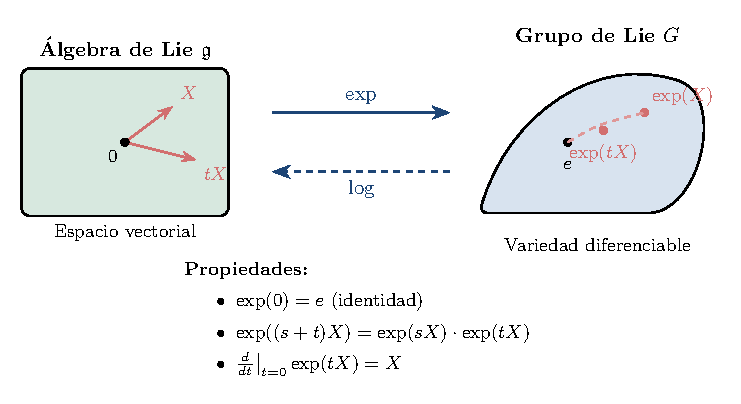
\includegraphics[width=0.7\textwidth]{images/exponential_map.pdf}
\caption[Mapa exponencial de grupos de Lie]{Mapa exponencial $\exp: \mathfrak{g} \to G$. Transforma vectores del álgebra de Lie (espacio tangente en la identidad $e$) en elementos del grupo de Lie, conectando la estructura lineal del álgebra con la estructura no lineal del grupo.}
\label{fig:exponential_map}
\end{figure}

\paragraph{Representaciones de Grupos de Lie}

La teoría de representaciones extiende el concepto de representación de grupo (\autoref{def:representacion_grupo}) al contexto diferenciable.

\begin{definition}[Representación de Grupo de Lie]\label{def:representacion_grupo_lie}
Sea $G$ un grupo de Lie y $V$ un espacio vectorial de dimensión finita. Una \textit{representación de $G$} es un homomorfismo de grupos de Lie:
\begin{equation}
\rho: G \rightarrow GL(V)
\end{equation}
es decir, $\rho$ es un homomorfismo de grupos que además es una aplicación suave.
\end{definition}

\begin{proposition}[Representación Inducida del Álgebra de Lie]\label{prop:representacion_algebra_lie}
Toda representación $\rho: G \rightarrow GL(V)$ de un grupo de Lie induce una \textit{representación del álgebra de Lie} $d\rho: \mathfrak{g} \rightarrow \mathfrak{gl}(V)$ definida por:
\begin{equation}
d\rho(X) = \frac{d}{dt}\Big|_{t=0} \rho(\exp(tX))
\end{equation}
Esta representación satisface $d\rho([X,Y]) = [d\rho(X), d\rho(Y)]$ (preserva el corchete de Lie).
\end{proposition}

\begin{proof}
\textbf{Buena definición.} Como $\rho$ es suave y $\exp: \mathfrak{g} \to G$ es suave, la composición $t \mapsto \rho(\exp(tX))$ es una curva suave en $GL(V)$. Su derivada en $t=0$ existe y pertenece a $\mathfrak{gl}(V) = T_{\text{Id}} GL(V)$.

\textbf{Linealidad.} Para $X, Y \in \mathfrak{g}$ y $\alpha \in \mathbb{R}$:
\[
d\rho(\alpha X) = \frac{d}{dt}\Big|_{t=0} \rho(\exp(t\alpha X)) = \alpha \frac{d}{ds}\Big|_{s=0} \rho(\exp(sX)) = \alpha\, d\rho(X)
\]
Para la aditividad, como $\exp(t(X+Y)) = \exp(tX)\exp(tY)\exp(-\tfrac{t^2}{2}[X,Y] + O(t^3))$ por la fórmula de Baker-Campbell-Hausdorff, al derivar en $t=0$ los términos de orden $\geq 2$ se anulan, y usando que $\rho$ es homomorfismo:
\[
d\rho(X+Y) = \frac{d}{dt}\Big|_{t=0} \rho(\exp(t(X+Y))) = \frac{d}{dt}\Big|_{t=0} \rho(\exp(tX))\rho(\exp(tY)) = d\rho(X) + d\rho(Y)
\]
donde la última igualdad se obtiene por la regla del producto para derivadas.

\textbf{Preservación del corchete.} La fórmula de Baker-Campbell-Hausdorff da:
\[
\exp(tX)\exp(tY)\exp(-tX)\exp(-tY) = \exp(t^2[X,Y] + O(t^3))
\]
Aplicando $\rho$ (que es homomorfismo) y derivando dos veces en $t=0$:
\[
\frac{d^2}{dt^2}\Big|_{t=0} \rho(\exp(t^2[X,Y] + O(t^3))) = d\rho([X,Y])
\]
Por otro lado, expandiendo el lado izquierdo con la regla del producto se obtiene $d\rho(X)d\rho(Y) - d\rho(Y)d\rho(X) = [d\rho(X), d\rho(Y)]$. Véase \citep[Theorem~3.28]{Kirillov2008} para los detalles completos.
\end{proof}

Esta correspondencia es fundamental en \gls{GDL}: permite optimizar en el espacio lineal $\mathfrak{g}$ (usando gradientes estándar) y luego aplicar transformaciones en el grupo $G$ mediante el mapa exponencial.

\begin{definition}[Representación Irreducible]\label{def:representacion_irreducible}
Una representación $\rho: G \rightarrow GL(V)$ es \textit{irreducible} si $V \neq \{0\}$ y los únicos subespacios de $V$ invariantes bajo la acción de $G$ son $\{0\}$ y $V$ mismo. Es decir, no existe un subespacio propio $W \subset V$ tal que $\rho(g)(W) \subseteq W$ para todo $g \in G$.
\end{definition}

Las representaciones irreducibles son los ``bloques fundamentales'' a partir de los cuales se construyen todas las demás representaciones.

\begin{example}[Representaciones Irreducibles de $SO(2)$]\label{ex:irreps_so2}
Las representaciones irreducibles de $SO(2)$ sobre $\mathbb{C}$ son unidimensionales, indexadas por $n \in \mathbb{Z}$:
\begin{equation}
\rho_n: SO(2) \rightarrow \mathbb{C}^*, \quad \rho_n(R_\theta) = e^{in\theta}
\end{equation}
Cada $\rho_n$ corresponde a una ``frecuencia'' en el análisis de Fourier circular (véase la \autoref{sec:analisis_armonico} del \autoref{ch:cnn}). En G-CNNs sobre imágenes rotadas, los canales de características se organizan según estas representaciones.
\end{example}

Los siguientes resultados fundamentales de teoría de representaciones requieren que el grupo sea \textit{compacto}:

\begin{definition}[Grupo Compacto]\label{def:grupo_compacto}
Un grupo de Lie $G$ es \textit{compacto} si es compacto como espacio topológico. Equivalentemente, $G$ es compacto si y solo si es cerrado y acotado en cualquier embedding en $\mathbb{R}^n$.
\end{definition}

Los grupos compactos más importantes en \gls{GDL} incluyen $SO(n)$, $O(n)$, $SU(n)$, $U(n)$, y todos los grupos finitos.

Los resultados que desarrollamos a continuación constituyen el análisis armónico de grupos compactos, generalizando el análisis de Fourier clásico (donde el grupo subyacente es $SO(2) \cong S^1$) a grupos de simetrías arbitrarios. La secuencia natural de construcción es: integración invariante sobre el grupo (medida de Haar), descomposición de representaciones en bloques irreducibles, unicidad de estos bloques (lema de Schur), funciones coordenadas y sus relaciones de ortogonalidad, y finalmente la completitud del sistema (teorema de Peter-Weyl). En \gls{GDL}, esta maquinaria proporciona la base teórica para implementar convoluciones equivariantes en el dominio espectral, transformando el problema de diseñar redes neuronales equivariantes en un problema algebraico bien estructurado.

\begin{definition}[Medida de Haar]\label{def:medida_haar_gdl}
Sea $G$ un grupo de Lie compacto. La \textit{medida de Haar} es la única medida $\mu$ sobre $G$ que satisface:
\begin{enumerate}
    \item \textbf{Invarianza}: $\mu(gA) = \mu(Ag) = \mu(A)$ para todo $g \in G$ y conjunto medible $A$
    \item \textbf{Normalización}: $\mu(G) = 1$
\end{enumerate}
Esta medida permite definir integrales sobre el grupo: $\int_G f(g) \, d\mu(g)$.
\end{definition}

La medida de Haar proporciona una forma canónica de ``promediar sobre todas las simetrías'' del grupo. En \gls{GDL}, este promediado es el mecanismo fundamental que subyace a las convoluciones de grupo: la convolución integra un filtro contra la señal usando precisamente la medida de Haar, y la invarianza de esta medida bajo traslaciones del grupo es lo que garantiza la equivarianza del operador resultante \citep{cohen2016groupequivariantconvolutional, kondor2018generalizationconvolutionalneural}.

\begin{theorem}[Descomposición de Representaciones]\label{thm:descomposicion_representaciones}
Toda representación de un grupo compacto $G$ sobre un espacio de Hilbert de dimensión finita se puede descomponer como suma directa de representaciones irreducibles:
\begin{equation}
V = \bigoplus_{i} n_i V_i
\end{equation}
donde cada $V_i$ es una representación irreducible y $n_i \in \mathbb{N}$ es su multiplicidad.
\end{theorem}

\begin{proof}
Sea $\rho: G \rightarrow GL(V)$ una representación de un grupo compacto $G$ sobre un espacio vectorial $V$ de dimensión finita. La demostración procede en tres pasos \citep{Fulton1991}.

\textbf{Paso 1: Producto interno $G$-invariante.}
Sea $\langle \cdot, \cdot \rangle_0$ un producto interno arbitrario en $V$. Definimos:
\begin{equation}\label{eq:producto_invariante}
\langle u, v \rangle = \int_G \langle \rho(g)u, \rho(g)v \rangle_0 \, d\mu(g)
\end{equation}
donde $\mu$ es la medida de Haar normalizada sobre $G$ (\autoref{def:medida_haar_gdl}). Verifiquemos que $\langle \cdot, \cdot \rangle$ es un producto interno $G$-invariante:
\begin{itemize}
    \item \textit{Linealidad y simetría}: se heredan de $\langle \cdot, \cdot \rangle_0$ y la linealidad de la integral.
    \item \textit{Positividad}: si $u \neq 0$, entonces $\rho(g)u \neq 0$ para todo $g$ (pues $\rho(g)$ es invertible), luego $\langle \rho(g)u, \rho(g)u \rangle_0 > 0$ para todo $g$, y la integral es estrictamente positiva.
    \item \textit{$G$-invarianza}: para cualquier $h \in G$,
    \[
    \langle \rho(h)u, \rho(h)v \rangle = \int_G \langle \rho(g)\rho(h)u, \rho(g)\rho(h)v \rangle_0 \, d\mu(g) = \int_G \langle \rho(gh)u, \rho(gh)v \rangle_0 \, d\mu(g).
    \]
    El cambio de variable $g' = gh$ y la invarianza de la medida de Haar dan $d\mu(g) = d\mu(g')$, luego esta integral es igual a $\langle u, v \rangle$.
\end{itemize}

\textbf{Paso 2: Complemento ortogonal invariante.}
Sea $W \subseteq V$ un subespacio $G$-invariante. Consideremos el complemento ortogonal $W^\perp$ respecto al producto interno $G$-invariante construido en el Paso~1. Para cualquier $v \in W^\perp$, $g \in G$ y $w \in W$:
\[
\langle \rho(g)v, w \rangle = \langle v, \rho(g^{-1})w \rangle = 0
\]
donde la primera igualdad usa la $G$-invarianza del producto interno (con $h = g^{-1}$) y la segunda se sigue de que $\rho(g^{-1})w \in W$ (pues $W$ es $G$-invariante) y $v \in W^\perp$. Por tanto $\rho(g)v \in W^\perp$, lo que prueba que $W^\perp$ es $G$-invariante.

\textbf{Paso 3: Inducción sobre $\dim(V)$.}
Procedemos por inducción fuerte sobre $n = \dim(V)$.

\textit{Caso base}: si $n = 1$, toda representación es irreducible (no existen subespacios propios no triviales) y $V$ es su propia descomposición.

\textit{Paso inductivo}: supongamos el resultado probado para todo espacio de dimensión menor que $n$. Si $\rho$ es irreducible, la descomposición es $V = V$ y no hay nada que probar. Si $\rho$ no es irreducible, existe un subespacio propio $G$-invariante $W \subset V$ con $0 < \dim(W) < n$. Por el Paso~2, $W^\perp$ es también $G$-invariante, y $V = W \oplus W^\perp$ con $\dim(W) < n$ y $\dim(W^\perp) < n$. Por hipótesis inductiva, tanto $W$ como $W^\perp$ se descomponen como sumas directas de representaciones irreducibles, y su unión proporciona la descomposición deseada de $V$.
\end{proof}

Este teorema garantiza que cualquier representación, por compleja que sea, puede analizarse en términos de sus componentes irreducibles. En \gls{GDL}, los mapas de características de una red equivariante son representaciones del grupo de simetría, y el teorema de descomposición garantiza que siempre pueden organizarse como sumas directas de ``canales de frecuencia'' irreducibles. Las redes steerable (véase \autoref{subsubsec:steerable_cnns_so2}) explotan este principio explícitamente, parametrizando las características como colecciones de representaciones irreducibles de distintos tipos \citep{weiler2018learningsteerable, cohen2016steerablecnns}.

El siguiente lema, debido a Issai Schur, es fundamental en teoría de representaciones:

\begin{lemma}[Schur]\label{lem:schur}
Sean $(\rho, V)$ y $(\sigma, W)$ representaciones irreducibles de un grupo $G$, y sea $T: V \to W$ un morfismo de representaciones (es decir, $T \circ \rho(g) = \sigma(g) \circ T$ para todo $g \in G$). Entonces:
\begin{enumerate}
    \item $T$ es un isomorfismo o $T = 0$.
    \item Si $V = W$ y el cuerpo base es $\mathbb{C}$, entonces $T = \lambda \cdot \mathrm{Id}$ para algún $\lambda \in \mathbb{C}$.
\end{enumerate}
\end{lemma}

\begin{proof}
\textbf{Parte 1.} Consideremos $\ker(T) \subseteq V$. Para cualquier $v \in \ker(T)$ y $g \in G$:
\[
T(\rho(g)v) = \sigma(g)T(v) = \sigma(g) \cdot 0 = 0
\]
Por tanto $\rho(g)v \in \ker(T)$, lo que muestra que $\ker(T)$ es un subespacio $G$-invariante de $V$. Como $\rho$ es irreducible, $\ker(T) = \{0\}$ o $\ker(T) = V$.

Análogamente, $\mathrm{Im}(T) \subseteq W$ es $G$-invariante: para $w = T(v) \in \mathrm{Im}(T)$,
\[
\sigma(g)w = \sigma(g)T(v) = T(\rho(g)v) \in \mathrm{Im}(T)
\]
Como $\sigma$ es irreducible, $\mathrm{Im}(T) = \{0\}$ o $\mathrm{Im}(T) = W$.

Si $\ker(T) = V$, entonces $T = 0$. Si $\ker(T) = \{0\}$ e $\mathrm{Im}(T) = W$, entonces $T$ es un isomorfismo.

\textbf{Parte 2.} Sea $\lambda$ un autovalor de $T$ (existe porque trabajamos sobre $\mathbb{C}$). Entonces $T - \lambda \cdot \mathrm{Id}$ es un morfismo de representaciones con núcleo no trivial. Por la Parte 1, $T - \lambda \cdot \mathrm{Id} = 0$.
\end{proof}

El lema de Schur restringe severamente la forma de las aplicaciones lineales equivariantes entre representaciones irreducibles: entre tipos distintos, toda aplicación equivariante es necesariamente cero; entre copias del mismo tipo, debe ser proporcional a la identidad. Para \gls{GDL}, esto implica que los parámetros aprendibles en capas equivariantes están fuertemente restringidos por la simetría del grupo, reduciendo drásticamente el espacio de parámetros respecto a arquitecturas sin restricciones \citep{cohen2016steerablecnns}. Esta restricción algebraica es precisamente la razón de la eficiencia en parámetros que exhiben las redes equivariantes.

\begin{definition}[Coeficientes Matriciales]\label{def:coeficientes_matriciales}
Sea $(\rho, V)$ una representación unitaria de dimensión finita de un grupo compacto $G$, con base ortonormal $\{e_1, \ldots, e_d\}$ donde $d = \dim(V)$. Los \textit{coeficientes matriciales} de $\rho$ son las funciones $\rho_{ij}: G \to \mathbb{C}$ definidas por:
\begin{equation}
\rho_{ij}(g) = \langle e_i, \rho(g) e_j \rangle
\end{equation}
Equivalentemente, $\rho_{ij}(g)$ es la entrada $(i,j)$ de la matriz que representa $\rho(g)$ en la base $\{e_i\}$.
\end{definition}

Los coeficientes matriciales son las ``funciones coordenadas'' de las representaciones. Para $SO(2)$, los coeficientes de $\rho_n(R_\theta) = e^{in\theta}$ son las funciones $e^{in\theta}$, que forman la base de Fourier. En general, los coeficientes matriciales juegan el papel de ``funciones base'' para la transformada de Fourier generalizada sobre el grupo, análogas a las exponenciales complejas $e^{in\theta}$ en el análisis de Fourier clásico. En métodos espectrales de \gls{GDL}, las convoluciones equivariantes sobre el grupo se convierten en multiplicaciones punto a punto en esta base espectral \citep{kondor2018generalizationconvolutionalneural}, permitiendo implementaciones computacionalmente eficientes.

\begin{proposition}[Relaciones de Ortogonalidad de Schur]\label{prop:ortogonalidad_schur}
Sean $(\rho, V)$ y $(\sigma, W)$ representaciones unitarias irreducibles de un grupo compacto $G$ con medida de Haar normalizada $\mu$. Entonces:
\begin{equation}\label{eq:ortogonalidad_schur}
\int_G \overline{\rho_{ij}(g)} \sigma_{kl}(g) \, d\mu(g) = \frac{\delta_{\rho\sigma} \delta_{ik} \delta_{jl}}{d_\rho}
\end{equation}
donde $d_\rho = \dim(V)$ y $\delta_{\rho\sigma} = 1$ si $\rho \cong \sigma$, y $0$ en caso contrario.
\end{proposition}

\begin{proof}
Definamos el operador $T: W \to V$ mediante:
\[
T = \int_G \rho(g) \circ P \circ \sigma(g^{-1}) \, d\mu(g)
\]
donde $P: W \to V$ es un operador lineal arbitrario. Por la invarianza de la medida de Haar, $T$ es un morfismo de representaciones: $\rho(h) T = T \sigma(h)$ para todo $h \in G$.

Por el Lema de Schur~\ref{lem:schur}: si $\rho \not\cong \sigma$, entonces $T = 0$; si $\rho = \sigma$, entonces $T = \lambda(P) \cdot \mathrm{Id}$.

Eligiendo $P$ como el operador $|e_l\rangle\langle e_j|$ y calculando la traza, se obtiene $\lambda = \delta_{jl}/d_\rho$, lo que da el resultado.
\end{proof}

Las relaciones de ortogonalidad garantizan que las componentes espectrales asociadas a distintas representaciones irreducibles están perfectamente separadas, sin interferencia cruzada. En arquitecturas equivariantes, esta independencia permite procesar distintos ``tipos de frecuencia'' en paralelo, de forma análoga al filtrado por bandas en procesamiento de señales clásico.

\begin{corollary}\label{cor:base_ortonormal_coeficientes}
Los coeficientes matriciales $\{\sqrt{d_\lambda} \rho^\lambda_{ij}\}$, donde $\lambda$ recorre $\widehat{G}$ y $1 \leq i,j \leq d_\lambda$, forman un sistema ortonormal en $L^2(G)$.
\end{corollary}

\begin{proof}
Consecuencia directa de las relaciones de ortogonalidad de Schur. Por la proposición anterior:
\[
\langle \rho^\lambda_{ij}, \rho^\mu_{kl} \rangle_{L^2(G)} = \frac{1}{d_\lambda} \delta_{\lambda\mu} \delta_{ik} \delta_{jl}
\]
Al normalizar por $\sqrt{d_\lambda}$, obtenemos:
\[
\langle \sqrt{d_\lambda}\, \rho^\lambda_{ij},\; \sqrt{d_\mu}\, \rho^\mu_{kl} \rangle = \sqrt{d_\lambda d_\mu} \cdot \frac{1}{d_\lambda} \delta_{\lambda\mu} \delta_{ik} \delta_{jl} = \delta_{\lambda\mu} \delta_{ik} \delta_{jl}
\]
lo que demuestra la ortonormalidad del sistema.
\end{proof}

Los resultados anteriores establecen que los coeficientes matriciales normalizados forman un sistema ortonormal en $L^2(G)$. El siguiente teorema completa el panorama mostrando que este sistema es además \textit{completo}: toda función de cuadrado integrable sobre el grupo puede recuperarse a partir de sus componentes espectrales, asegurando que la descomposición de Fourier generalizada (que extiende la transformada clásica, \autoref{def:transformada_fourier_continua}) no pierde información.

\begin{theorem}[Peter-Weyl]\label{thm:peter_weyl}
Sea $G$ un grupo de Lie compacto. El espacio $L^2(G)$ de funciones de cuadrado integrable sobre $G$ se descompone como:
\begin{equation}
L^2(G) = \bigoplus_{\lambda \in \widehat{G}} d_\lambda \cdot V_\lambda
\end{equation}
donde $\widehat{G}$ es el conjunto de clases de equivalencia de representaciones irreducibles, $V_\lambda$ es el espacio de la representación $\lambda$, y $d_\lambda = \dim(V_\lambda)$ es su dimensión.
\end{theorem}

\begin{proof}
La demostración procede en dos pasos.

\textbf{Paso 1: Ortogonalidad.} Por el \autoref{cor:base_ortonormal_coeficientes}, los coeficientes matriciales normalizados $\{\sqrt{d_\lambda} \rho^\lambda_{ij}\}$ forman un sistema ortonormal en $L^2(G)$.

\textbf{Paso 2: Completitud.} Sea $f \in L^2(G)$ ortogonal a todos los coeficientes matriciales. Definamos el operador $T_f: V_\lambda \to V_\lambda$ por:
\[
T_f = \int_G f(g) \rho^\lambda(g) \, d\mu(g)
\]
Para cada $v, w \in V_\lambda$:
\[
\langle w, T_f v \rangle = \int_G f(g) \langle w, \rho^\lambda(g) v \rangle \, d\mu(g) = \int_G f(g) \rho^\lambda_{wv}(g) \, d\mu(g) = 0
\]
donde la última igualdad usa que $f$ es ortogonal a todos los coeficientes matriciales. Como esto vale para todo $v, w$, tenemos $T_f = 0$ para toda representación $\lambda$.

El paso clave es mostrar que $T_f = 0$ para toda $\lambda$ implica $f = 0$. Esto se sigue del hecho de que las representaciones de $G$ separan puntos: si $g \neq h$, existe $\lambda$ tal que $\rho^\lambda(g) \neq \rho^\lambda(h)$. Combinando con el teorema de Stone-Weierstrass para grupos compactos, los coeficientes matriciales son densos en $C(G)$, y por tanto en $L^2(G)$.

Así, el sistema ortonormal de coeficientes matriciales es completo, lo que establece la descomposición.
\end{proof}

El teorema de Peter-Weyl es la generalización de la serie de Fourier a grupos no abelianos. Para $G = SO(2)$, recuperamos la descomposición de Fourier clásica: las representaciones irreducibles son $\rho_n(R_\theta) = e^{in\theta}$ para $n \in \mathbb{Z}$, y la descomposición se convierte en la serie de Fourier $f(\theta) = \sum_{n \in \mathbb{Z}} c_n e^{in\theta}$ (para un desarrollo detallado de las series y la transformada de Fourier, véase la Sección~\ref{subsec:fundamentos_fourier} del \autoref{ch:cnn}).

\textbf{Implicaciones para GDL.} El teorema de Peter-Weyl tiene consecuencias directas para el diseño de arquitecturas neuronales equivariantes:
\begin{itemize}
    \item \textbf{Estructura de canales}: Cada representación irreducible $V_\lambda$ corresponde a un ``tipo'' de canal en G-CNNs.
    \item \textbf{Dimensiones determinadas}: Las dimensiones $d_\lambda$ de las capas no son arbitrarias, sino que están fijadas por la estructura del grupo.
    \item \textbf{Convoluciones en frecuencia}: Las convoluciones equivariantes se implementan eficientemente en el dominio de Fourier generalizado, multiplicando coeficientes en cada $V_\lambda$.
\end{itemize}

\begin{corollary}[Estructura de canales en G-CNNs]\label{cor:peter_weyl_gcnn}
	Sea $G$ un grupo de Lie compacto y $\Phi: L^2(G) \to L^2(G)$ un operador lineal $G$-equivariante. Por el teorema de Peter-Weyl, $\Phi$ preserva la descomposición en irreducibles:
	\[
		\Phi = \bigoplus_{\lambda \in \widehat{G}} \Phi_\lambda, \quad \text{donde } \Phi_\lambda: d_\lambda V_\lambda \to d_\lambda V_\lambda
	\]
	Cada $\Phi_\lambda$ actúa como $\Phi_\lambda = I_{d_\lambda} \otimes W_\lambda$ para alguna matriz $W_\lambda \in \mathbb{R}^{d_\lambda \times d_\lambda}$.

	Consecuencias para arquitecturas G-equivariantes (desarrolladas en el \autoref{ch:cnn}):
	\begin{enumerate}
		\item Los ``canales'' de una capa equivariante son indexados por representaciones irreducibles $\lambda \in \widehat{G}$
		\item El número de parámetros aprendibles por canal es $d_\lambda^2$, independiente de la resolución de entrada
		\item La equivarianza se garantiza automáticamente al trabajar en el dominio espectral
	\end{enumerate}
\end{corollary}

\begin{proof}
Por el \autoref{thm:peter_weyl}, $L^2(G) = \bigoplus_{\lambda \in \widehat{G}} d_\lambda V_\lambda$. Sea $\Phi: L^2(G) \to L^2(G)$ un operador lineal $G$-equivariante, es decir, $\Phi \circ L_g = L_g \circ \Phi$ para todo $g \in G$, donde $L_g$ es la representación regular izquierda. Como $\Phi$ conmuta con la acción de $G$, debe preservar cada sumando isótipico $d_\lambda V_\lambda$, pues estos son los subespacios $G$-invariantes irreducibles de $L^2(G)$. Así, $\Phi = \bigoplus_\lambda \Phi_\lambda$ con $\Phi_\lambda: d_\lambda V_\lambda \to d_\lambda V_\lambda$.

Dentro del sumando $d_\lambda V_\lambda \cong V_\lambda \otimes \mathbb{R}^{d_\lambda}$, la acción de $G$ es $\rho^\lambda \otimes I_{d_\lambda}$. Por el Lema de Schur~\ref{lem:schur}, todo endomorfismo $G$-equivariante de $V_\lambda \otimes \mathbb{R}^{d_\lambda}$ tiene la forma $I_{d_\lambda} \otimes W_\lambda$ para alguna matriz $W_\lambda \in \mathbb{R}^{d_\lambda \times d_\lambda}$, lo que establece la estructura de canales descrita.
\end{proof}

\begin{example}[Descomposición de Fourier en $SO(2)$: Conexión con CNNs clásicas]\label{ex:peter_weyl_so2_detallado}
	Para $G = SO(2) \cong S^1$, el grupo abeliano de rotaciones en el plano, la descomposición de Peter-Weyl se reduce a la serie de Fourier clásica.

	\textbf{Representaciones irreducibles:} Todas las irreducibles de $SO(2)$ son unidimensionales ($d_n = 1$ para todo $n$), dadas por:
	\[
		\rho_n: SO(2) \to \mathbb{C}^*, \quad \rho_n(R_\theta) = e^{in\theta}, \quad n \in \mathbb{Z}
	\]

	\textbf{Descomposición:} Toda función $f \in L^2(SO(2)) \cong L^2([0, 2\pi])$ se descompone como:
	\[
		f(\theta) = \sum_{n \in \mathbb{Z}} \hat{f}_n e^{in\theta}, \quad \hat{f}_n = \frac{1}{2\pi} \int_0^{2\pi} f(\theta) e^{-in\theta} d\theta
	\]

	\textbf{Conexión con CNNs cíclicas:} Para señales discretas sobre $\mathbb{Z}_N$ (versión discreta de $SO(2)$), la convolución circular se computa en el dominio de Fourier mediante la DFT:
	\[
		(f \star g)[k] = \text{IDFT}(\text{DFT}(f) \odot \text{DFT}(g))
	\]
	donde $\odot$ es el producto elemento a elemento. Esta es exactamente la implementación eficiente de CNNs cíclicas usando FFT, un caso especial del Teorema de Convolución en Dominio de Fourier (\autoref{thm:convolucion_fourier} del \autoref{ch:cnn}).
\end{example}

\subsubsection{Grupos de Lie Fundamentales}\label{subsubsec:grupos_lie_fundamentales}

A continuación desarrollamos los grupos de Lie más relevantes para \gls{GDL}, presentando sus definiciones formales, parametrizaciones explícitas y álgebras de Lie asociadas. Para cada grupo, derivamos su dimensión como aplicación de una herramienta general que presentamos primero.

\begin{remark}[Dimensión de un grupo de Lie]\label{rem:dimension_grupo_lie}
La \textbf{dimensión} de un grupo de Lie $G$ es su dimensión como variedad diferenciable (\autoref{def:variedad_diferenciable}), que coincide con la dimensión de su álgebra de Lie: $\dim G = \dim \mathfrak{g} = \dim T_eG$.

Esta dimensión tiene una interpretación directa en el contexto del \gls{GDL}, en conexión con la hipótesis de la variedad (\autoref{subsec:hipotesis_variedad}): la dimensión del grupo de simetría cuantifica los grados de libertad de las transformaciones que preservan la estructura de los datos. Si una señal en $\mathbb{R}^d$ es invariante bajo la acción de un grupo $G$ de dimensión $k$, la señal reside efectivamente en una variedad de dimensión $\leq d - k$, ya que $k$ grados de libertad quedan fijados por la simetría. Cuantas más simetrías respetan los datos, mayor es la reducción dimensional.
\end{remark}

\begin{proposition}[Dimensión de subgrupos matriciales]\label{prop:dimension_subgrupos_matriciales}
Sea $F: \mathbb{R}^{n \times n} \to \mathbb{R}^k$ una aplicación suave y $c \in \mathbb{R}^k$ un valor regular de $F$ (véase \autoref{def:valor_regular} del \autoref{ch:teoremas_complementarios}). Entonces $F^{-1}(c)$ es una subvariedad diferenciable de $\mathbb{R}^{n \times n}$ de dimensión $n^2 - k$.
\end{proposition}

\begin{proof}
Es una aplicación directa del Teorema del Nivel Regular (\autoref{thm:nivel_regular} del \autoref{ch:teoremas_complementarios}; véase también \citep[Capítulo~5]{lee2012introduction}). Al ser $c$ un valor regular, el diferencial $dF_A$ tiene rango $k$ en todo punto $A \in F^{-1}(c)$, por lo que $F^{-1}(c)$ es una subvariedad suave de dimensión $n^2 - k$. El mismo argumento se aplica sobre $\mathbb{C}^{n \times n} \cong \mathbb{R}^{2n^2}$ para grupos unitarios.
\end{proof}

\paragraph{Grupo Ortogonal Especial $SO(n)$}

\begin{definition}[Grupo Ortogonal Especial]\label{def:grupo_so_n}
El \textit{grupo ortogonal especial} $SO(n)$ es el grupo de matrices ortogonales con determinante $1$:
\begin{equation}
SO(n) = \{R \in \mathbb{R}^{n \times n} : R^T R = I_n, \det(R) = 1\}
\end{equation}
con la operación de multiplicación matricial. Es un grupo de Lie compacto de dimensión $\frac{n(n-1)}{2}$.
\end{definition}

Derivamos esta dimensión como aplicación de la \autoref{prop:dimension_subgrupos_matriciales}. Consideremos la aplicación $F: \mathbb{R}^{n \times n} \to \operatorname{Sym}(n)$ definida por $F(R) = R^T R - I_n$, donde $\operatorname{Sym}(n)$ denota el espacio de matrices simétricas $n \times n$, de dimensión $\frac{n(n+1)}{2}$ ($n$ entradas diagonales y $\binom{n}{2}$ entradas sobre la diagonal). Entonces $O(n) = F^{-1}(0)$.

Para verificar que $0$ es valor regular, calculamos el diferencial: $dF_R(H) = H^T R + R^T H$. Dada cualquier $S \in \operatorname{Sym}(n)$, la elección $H = \frac{1}{2}RS$ satisface
\[
	dF_R(H) = \tfrac{1}{2}S^T R^T R + \tfrac{1}{2}R^T R S = \tfrac{1}{2}S + \tfrac{1}{2}S = S
\]
usando $R^T R = I_n$ y $S^T = S$, lo que demuestra la sobreyectividad de $dF_R$. Por tanto:
\[
	\dim O(n) = n^2 - \frac{n(n+1)}{2} = \frac{n(n-1)}{2}
\]
La condición adicional $\det(R) = 1$ selecciona la componente conexa de la identidad dentro de $O(n)$: dado que $\det: O(n) \to \{-1, +1\}$ es una función discreta, no impone restricción diferencial, y $\dim SO(n) = \dim O(n) = \frac{n(n-1)}{2}$. Como verificación, el álgebra de Lie $\mathfrak{so}(n) = \{A \in \mathbb{R}^{n \times n} : A^T + A = 0\}$ de matrices antisimétricas tiene exactamente $\binom{n}{2} = \frac{n(n-1)}{2}$ entradas libres (las situadas estrictamente sobre la diagonal).

\begin{definition}[Grupo Ortogonal]\label{def:grupo_o_n}
El \textit{grupo ortogonal} $O(n)$ es el grupo de todas las matrices ortogonales:
\begin{equation}
O(n) = \{R \in \mathbb{R}^{n \times n} : R^T R = I_n\}
\end{equation}
Incluye tanto rotaciones ($\det R = +1$) como reflexiones ($\det R = -1$), por lo que $SO(n) \subset O(n)$ es el subgrupo de índice 2 formado por las transformaciones que preservan orientación. Es un grupo de Lie compacto de dimensión $\frac{n(n-1)}{2}$.
\end{definition}

\begin{example}[$SO(2)$: Rotaciones en el Plano]\label{ex:so2_rotaciones}
El grupo $SO(2)$ parametriza las rotaciones en $\mathbb{R}^2$. Cada elemento se representa mediante un ángulo $\theta \in [0, 2\pi)$:
\begin{equation}
R_\theta = \begin{pmatrix}
\cos\theta & -\sin\theta \\
\sin\theta & \cos\theta
\end{pmatrix}
\end{equation}
Por ejemplo, una rotación de $90^\circ$ corresponde a:
\begin{equation}
R_{\pi/2} = \begin{pmatrix}
0 & -1 \\
1 & 0
\end{pmatrix}
\end{equation}
Topológicamente, $SO(2) \cong S^1$ (el círculo). Su álgebra de Lie $\mathfrak{so}(2)$ es unidimensional, generada por:
\begin{equation}
J = \begin{pmatrix}
0 & -1 \\
1 & 0
\end{pmatrix}, \quad \text{con } e^{\theta J} = R_\theta
\end{equation}
\end{example}

\begin{figure}[htbp]
\centering
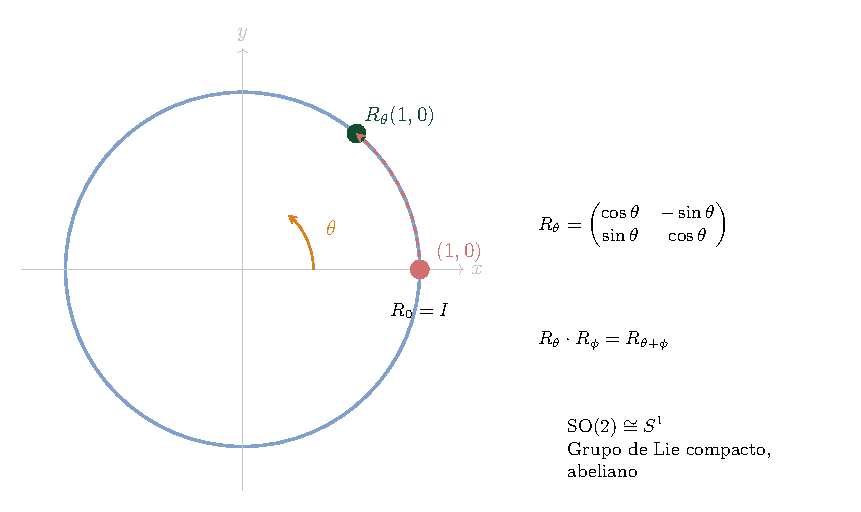
\includegraphics[width=0.6\textwidth]{images/so2_rotations.pdf}
\caption[Rotaciones en el plano: $SO(2)$]{El grupo $SO(2)$ de rotaciones en el plano. Cada elemento $R_\theta$ rota vectores por un ángulo $\theta$. Topológicamente, $SO(2)$ es isomorfo al círculo $S^1$.}
\label{fig:so2_rotations}
\end{figure}

\begin{example}[$SO(3)$: Rotaciones en el Espacio]\label{ex:so3_rotaciones}
El grupo $SO(3)$ describe las rotaciones en $\mathbb{R}^3$, fundamental para procesamiento de datos 3D. Las rotaciones elementales alrededor de los ejes coordenados son:
\begin{align}
R_x(\theta) &= \begin{pmatrix}
1 & 0 & 0 \\
0 & \cos\theta & -\sin\theta \\
0 & \sin\theta & \cos\theta
\end{pmatrix}, \quad
R_y(\theta) = \begin{pmatrix}
\cos\theta & 0 & \sin\theta \\
0 & 1 & 0 \\
-\sin\theta & 0 & \cos\theta
\end{pmatrix}, \\
R_z(\theta) &= \begin{pmatrix}
\cos\theta & -\sin\theta & 0 \\
\sin\theta & \cos\theta & 0 \\
0 & 0 & 1
\end{pmatrix}
\end{align}
El álgebra de Lie $\mathfrak{so}(3)$ consiste en matrices antisimétricas $3 \times 3$, con base:
\begin{equation}
L_x = \begin{pmatrix}
0 & 0 & 0 \\
0 & 0 & -1 \\
0 & 1 & 0
\end{pmatrix}, \quad
L_y = \begin{pmatrix}
0 & 0 & 1 \\
0 & 0 & 0 \\
-1 & 0 & 0
\end{pmatrix}, \quad
L_z = \begin{pmatrix}
0 & -1 & 0 \\
1 & 0 & 0 \\
0 & 0 & 0
\end{pmatrix}
\end{equation}
El corchete de Lie satisface $[L_i, L_j] = \epsilon_{ijk} L_k$, donde $\epsilon_{ijk}$ es el símbolo de Levi-Civita.
\end{example}

\begin{example}[Mapa exponencial en $SO(3)$: Fórmula de Rodrigues]\label{ex:mapa_exp_so3}
	El mapa exponencial $\exp: \mathfrak{so}(3) \to SO(3)$ tiene una forma cerrada conocida como la \textbf{fórmula de Rodrigues}. Para un vector $\boldsymbol{\omega} = (\omega_1, \omega_2, \omega_3)^T \in \mathbb{R}^3$ con $\theta = \|\boldsymbol{\omega}\|$, definimos la matriz antisimétrica:
	\[
		[\boldsymbol{\omega}]_\times = \begin{pmatrix}
			0 & -\omega_3 & \omega_2 \\
			\omega_3 & 0 & -\omega_1 \\
			-\omega_2 & \omega_1 & 0
		\end{pmatrix} \in \mathfrak{so}(3)
	\]
	Entonces el mapa exponencial es:
	\begin{equation}\label{eq:rodrigues}
		\exp([\boldsymbol{\omega}]_\times) = I + \frac{\sin\theta}{\theta} [\boldsymbol{\omega}]_\times + \frac{1 - \cos\theta}{\theta^2} [\boldsymbol{\omega}]_\times^2
	\end{equation}

	\textbf{Ejemplo numérico:} Consideremos una rotación de $90^\circ$ alrededor del eje $z$, es decir, $\boldsymbol{\omega} = (0, 0, \pi/2)^T$. Entonces $\theta = \pi/2$ y:
	\[
		[\boldsymbol{\omega}]_\times = \frac{\pi}{2} \begin{pmatrix}
			0 & -1 & 0 \\
			1 & 0 & 0 \\
			0 & 0 & 0
		\end{pmatrix}
	\]
	Aplicando la fórmula de Rodrigues con $\sin(\pi/2) = 1$ y $\cos(\pi/2) = 0$:
	\begin{align*}
		\exp([\boldsymbol{\omega}]_\times) &= I + \frac{2}{\pi} \cdot \frac{\pi}{2} \begin{pmatrix}
			0 & -1 & 0 \\
			1 & 0 & 0 \\
			0 & 0 & 0
		\end{pmatrix} + \frac{4}{\pi^2} \cdot \frac{\pi^2}{4} \begin{pmatrix}
			-1 & 0 & 0 \\
			0 & -1 & 0 \\
			0 & 0 & 0
		\end{pmatrix} \\
		&= \begin{pmatrix}
			0 & -1 & 0 \\
			1 & 0 & 0 \\
			0 & 0 & 1
		\end{pmatrix} = R_z(\pi/2)
	\end{align*}

	\textbf{Relevancia para GDL:} La fórmula de Rodrigues es computacionalmente eficiente y evita la singularidad de los ángulos de Euler. Es fundamental para:
	\begin{itemize}
		\item Redes $SE(3)$-equivariantes que procesan nubes de puntos 3D
		\item Interpolación suave de rotaciones en animación y robótica
		\item Parametrización del espacio de rotaciones en optimización
	\end{itemize}
\end{example}

\begin{figure}[htbp]
\centering
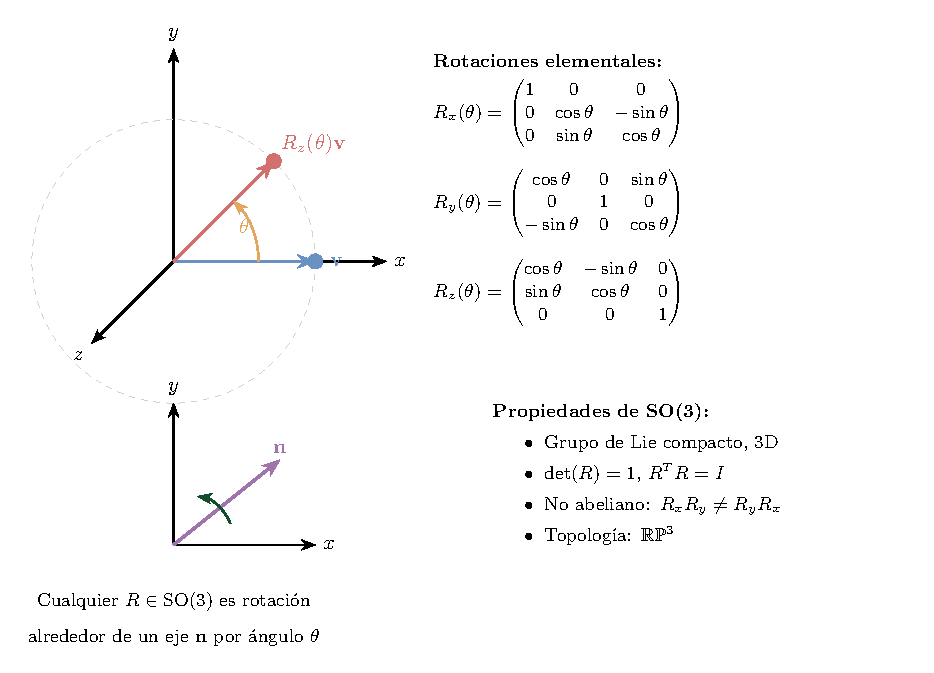
\includegraphics[width=0.75\textwidth]{images/so3_rotations.pdf}
\caption[Rotaciones en el espacio: $SO(3)$]{El grupo $SO(3)$ de rotaciones en el espacio tridimensional. Las matrices de rotación elementales $R_x$, $R_y$ y $R_z$ rotan alrededor de los ejes coordenados. Topológicamente, $SO(3) \cong \mathbb{RP}^3$.}
\label{fig:so3_rotations}
\end{figure}

\paragraph{Grupo Euclidiano Especial $SE(n)$}

\begin{definition}[Grupo Euclidiano Especial]\label{def:grupo_se_n}
El \textit{grupo euclidiano especial} $SE(n)$ es el grupo de transformaciones rígidas en $\mathbb{R}^n$ (rotación + traslación). Se define como el producto semidirecto (\autoref{def:producto_semidirecto}):
\begin{equation}
SE(n) = \mathbb{R}^n \rtimes SO(n)
\end{equation}
donde la operación de grupo es $(t_1, R_1) \cdot (t_2, R_2) = (t_1 + R_1 t_2, R_1 R_2)$.
Es un grupo de Lie de dimensión $\frac{n(n-1)}{2} + n = \frac{n(n+1)}{2}$.
\end{definition}

\begin{definition}[Grupo Euclidiano]\label{def:grupo_e_n}
El \textit{grupo euclidiano} $E(n)$ es el grupo de todas las isometrías de $\mathbb{R}^n$ (rotaciones, reflexiones y traslaciones). Se define como el producto semidirecto:
\begin{equation}
E(n) = \mathbb{R}^n \rtimes O(n)
\end{equation}
donde $O(n)$ es el grupo ortogonal (\autoref{def:grupo_o_n}). A diferencia de $SE(n)$, que solo incluye rotaciones y traslaciones, $E(n)$ incluye también reflexiones. Es un grupo de Lie de dimensión $\frac{n(n+1)}{2}$.
\end{definition}

\begin{example}[$SE(3)$ en Coordenadas Homogéneas]\label{ex:se3_homogeneas}
Las transformaciones de $SE(3)$ se representan convenientemente como matrices $4 \times 4$ en coordenadas homogéneas:
\begin{equation}
T = \begin{pmatrix}
R & t \\
0 & 1
\end{pmatrix} \in \mathbb{R}^{4 \times 4}, \quad R \in SO(3), \, t \in \mathbb{R}^3
\end{equation}
La acción sobre un punto $\mathbf{x} \in \mathbb{R}^3$ es:
\begin{equation}
\begin{pmatrix}
R & t \\
0 & 1
\end{pmatrix}
\begin{pmatrix}
\mathbf{x} \\
1
\end{pmatrix}
= \begin{pmatrix}
R\mathbf{x} + t \\
1
\end{pmatrix}
\end{equation}
El álgebra de Lie $\mathfrak{se}(3)$ tiene dimensión 6, con generadores para rotaciones $(L_x, L_y, L_z)$ y traslaciones $(P_x, P_y, P_z)$:
\begin{equation}
P_x = \begin{pmatrix}
0 & 0 & 0 & 1 \\
0 & 0 & 0 & 0 \\
0 & 0 & 0 & 0 \\
0 & 0 & 0 & 0
\end{pmatrix}, \quad
P_y = \begin{pmatrix}
0 & 0 & 0 & 0 \\
0 & 0 & 0 & 1 \\
0 & 0 & 0 & 0 \\
0 & 0 & 0 & 0
\end{pmatrix}, \quad
P_z = \begin{pmatrix}
0 & 0 & 0 & 0 \\
0 & 0 & 0 & 0 \\
0 & 0 & 0 & 1 \\
0 & 0 & 0 & 0
\end{pmatrix}
\end{equation}
En \gls{GDL}, $SE(3)$ es esencial para nubes de puntos 3D y datos moleculares, donde las predicciones deben ser invariantes a transformaciones rígidas.
\end{example}

\paragraph{Grupos Lineales $GL(n)$ y $SL(n)$}

\begin{definition}[Grupo Lineal General]\label{def:grupo_gl_n}
El \textit{grupo lineal general} $GL(n, \mathbb{R})$ es el grupo de matrices invertibles $n \times n$:
\begin{equation}
GL(n, \mathbb{R}) = \{A \in \mathbb{R}^{n \times n} : \det(A) \neq 0\}
\end{equation}
Es un grupo de Lie no compacto de dimensión $n^2$. Su álgebra de Lie $\mathfrak{gl}(n, \mathbb{R})$ es el espacio de todas las matrices $n \times n$, con el corchete $[A, B] = AB - BA$.
\end{definition}

\begin{definition}[Grupo Lineal Especial]\label{def:grupo_sl_n}
El \textit{grupo lineal especial} $SL(n, \mathbb{R})$ es el subgrupo de matrices con determinante $1$:
\begin{equation}
SL(n, \mathbb{R}) = \{A \in GL(n, \mathbb{R}) : \det(A) = 1\}
\end{equation}
Es un grupo de Lie de dimensión $n^2 - 1$. Su álgebra de Lie $\mathfrak{sl}(n, \mathbb{R})$ consiste en matrices de traza cero.
\end{definition}

Las dimensiones de estos grupos se obtienen por métodos distintos. Para $GL(n, \mathbb{R})$: como $\det: \mathbb{R}^{n \times n} \to \mathbb{R}$ es un polinomio en las entradas (y por tanto continua), $GL(n, \mathbb{R}) = \det^{-1}(\mathbb{R} \setminus \{0\})$ es la preimagen de un abierto, luego es un abierto de $\mathbb{R}^{n \times n}$. Un abierto de $\mathbb{R}^{n^2}$ hereda la estructura de variedad con la misma dimensión $n^2$.

Para $SL(n, \mathbb{R})$, aplicamos la \autoref{prop:dimension_subgrupos_matriciales} con $F = \det$ y $c = 1$. El diferencial del determinante es $d(\det)_A(H) = \det(A) \cdot \operatorname{tr}(A^{-1}H)$. Para $A \in SL(n)$, $\det(A) = 1$, y la aplicación $H \mapsto \operatorname{tr}(A^{-1}H)$ es sobreyectiva sobre $\mathbb{R}$: basta tomar $H = tA$ para obtener $\operatorname{tr}(I_n) \cdot t = nt$. Así $1$ es valor regular y $\dim SL(n) = n^2 - 1$. Como verificación, $\mathfrak{sl}(n, \mathbb{R}) = \{A : \operatorname{tr}(A) = 0\}$ impone una restricción lineal sobre $\mathfrak{gl}(n, \mathbb{R}) \cong \mathbb{R}^{n^2}$, dejando dimensión $n^2 - 1$.

\paragraph{Grupos Unitarios $U(n)$ y $SU(n)$}

\begin{definition}[Grupo Unitario]\label{def:grupo_u_n}
El \textit{grupo unitario} $U(n)$ es el grupo de matrices unitarias $n \times n$:
\begin{equation}
U(n) = \{U \in \mathbb{C}^{n \times n} : U^\dagger U = I_n\}
\end{equation}
donde $U^\dagger = \overline{U}^T$ denota la conjugada traspuesta. Es un grupo de Lie compacto de dimensión $n^2$.
\end{definition}

\begin{definition}[Grupo Unitario Especial]\label{def:grupo_su_n}
El \textit{grupo unitario especial} $SU(n)$ es el subgrupo de matrices unitarias con determinante $1$:
\begin{equation}
SU(n) = \{U \in U(n) : \det(U) = 1\}
\end{equation}
Es un grupo de Lie compacto de dimensión $n^2 - 1$.
\end{definition}

Derivamos las dimensiones de $U(n)$ y $SU(n)$. Para $U(n)$, definimos $F: \mathbb{C}^{n \times n} \to \operatorname{Herm}(n)$ por $F(U) = U^\dagger U - I_n$, donde $\operatorname{Herm}(n)$ denota el espacio de matrices hermitianas $n \times n$. Este espacio tiene dimensión real $n^2$: las $n$ entradas diagonales son reales, y las $\binom{n}{2}$ entradas sobre la diagonal son complejas ($n(n-1)$ parámetros reales), sumando $n + n(n-1) = n^2$. El espacio ambiente $\mathbb{C}^{n \times n}$ tiene dimensión real $2n^2$. El diferencial es $dF_U(H) = H^\dagger U + U^\dagger H$; para cualquier $S \in \operatorname{Herm}(n)$, la elección $H = \frac{1}{2}US$ satisface $dF_U(H) = S$ (análogamente al caso ortogonal, usando $U^\dagger U = I_n$ y $S^\dagger = S$). Por la \autoref{prop:dimension_subgrupos_matriciales}:
\[
	\dim U(n) = 2n^2 - n^2 = n^2
\]

Para $SU(n)$, la restricción adicional $\det(U) = 1$ impone una condición suave sobre $U(n)$. Para $U$ unitaria, $|\det(U)| = 1$, así que $\det: U(n) \to S^1$. El diferencial $d(\det)_U$ restringido a $T_U U(n)$ es sobreyectivo sobre $T_{\det(U)}S^1 \cong i\mathbb{R}$: para $X \in \mathfrak{u}(n)$, $d(\det)_I(X) = \operatorname{tr}(X)$, que es sobreyectivo (basta tomar $X = itI_n$). Como $S^1$ tiene dimensión real $1$, la condición $\det = 1$ define una subvariedad de codimensión $1$, luego $\dim SU(n) = n^2 - 1$.

\begin{example}[$SU(2)$ y su Relación con $SO(3)$]\label{ex:su2_so3}
El grupo $SU(2)$ consiste en matrices $2 \times 2$ de la forma:
\begin{equation}
U = \begin{pmatrix}
\alpha & -\overline{\beta} \\
\beta & \overline{\alpha}
\end{pmatrix}, \quad |\alpha|^2 + |\beta|^2 = 1
\end{equation}
Topológicamente, $SU(2) \cong S^3$ (la 3-esfera). Vamos a construir explícitamente un homomorfismo sobreyectivo $\pi: SU(2) \to SO(3)$ y a demostrar que $SO(3) \cong SU(2)/\mathbb{Z}_2$.

\textbf{El álgebra de Lie $\mathfrak{su}(2)$ y su producto interno.}
El álgebra de Lie $\mathfrak{su}(2)$ consiste en las matrices antihermitanas de traza cero:
\[
	\mathfrak{su}(2) = \{X \in M_2(\mathbb{C}) : X^\dagger = -X, \; \operatorname{tr}(X) = 0\}
\]
Las \textit{matrices de Pauli} proporcionan una base natural:
\begin{equation}
\sigma_x = \begin{pmatrix}
0 & 1 \\
1 & 0
\end{pmatrix}, \quad
\sigma_y = \begin{pmatrix}
0 & -i \\
i & 0
\end{pmatrix}, \quad
\sigma_z = \begin{pmatrix}
1 & 0 \\
0 & -1
\end{pmatrix}
\end{equation}
Los generadores $\tau_k = \frac{i}{2}\sigma_k$ para $k \in \{x, y, z\}$ forman una base de $\mathfrak{su}(2)$ y satisfacen $[\tau_i, \tau_j] = \epsilon_{ijk}\tau_k$. Dotamos a $\mathfrak{su}(2)$ del producto interno:
\begin{equation}\label{eq:inner_product_su2}
	\langle X, Y \rangle = -2\operatorname{tr}(XY)
\end{equation}
Para verificar que $\{\tau_1, \tau_2, \tau_3\}$ es base ortonormal, calculamos $\langle \tau_j, \tau_k \rangle = -2\operatorname{tr}(\tau_j \tau_k) = \frac{1}{2}\operatorname{tr}(\sigma_j \sigma_k) = \delta_{jk}$, donde la última igualdad usa la identidad de Pauli $\sigma_j \sigma_k = \delta_{jk} I + i\epsilon_{jkl}\sigma_l$ y $\operatorname{tr}(\sigma_l) = 0$.

\textbf{Construcción de $\pi$ vía la acción adjunta.}
Para cada $U \in SU(2)$, definimos la representación adjunta $\operatorname{Ad}_U: \mathfrak{su}(2) \to \mathfrak{su}(2)$ por:
\begin{equation}\label{eq:adjoint_su2}
	\operatorname{Ad}_U(X) = UXU^\dagger
\end{equation}
Veamos que $\operatorname{Ad}_U$ preserva $\mathfrak{su}(2)$: si $X^\dagger = -X$ y $\operatorname{tr}(X) = 0$, entonces $(UXU^\dagger)^\dagger = UX^\dagger U^\dagger = -UXU^\dagger$ y $\operatorname{tr}(UXU^\dagger) = \operatorname{tr}(X) = 0$. Además, $\operatorname{Ad}_U$ preserva el producto interno:
\[
	\langle UXU^\dagger, UYU^\dagger \rangle = -2\operatorname{tr}(UXU^\dagger \cdot UYU^\dagger) = -2\operatorname{tr}(UXYU^\dagger) = -2\operatorname{tr}(XY) = \langle X, Y \rangle
\]
Definimos $\pi(U)$ como la matriz de $\operatorname{Ad}_U$ en la base ortonormal $\{\tau_1, \tau_2, \tau_3\}$, es decir, $[\pi(U)]_{jk} = \langle \tau_j, \operatorname{Ad}_U(\tau_k) \rangle$. Como $\operatorname{Ad}_U$ preserva el producto interno, $\pi(U) \in O(3)$. El grupo $SU(2)$ es conexo (es homeomorfo a $S^3$), $\pi$ es continuo y $\pi(I) = I_3 \in SO(3)$. Como $\det \circ\, \pi: SU(2) \to \{-1, +1\}$ es continua sobre un espacio conexo, debe ser constante, luego $\det(\pi(U)) = 1$ para todo $U$. Concluimos que $\pi: SU(2) \to SO(3)$ es un homomorfismo de grupos, ya que $\operatorname{Ad}_{UV} = \operatorname{Ad}_U \circ \operatorname{Ad}_V$.

\textbf{Cálculo del kernel.}
Determinamos $\ker(\pi) = \{U \in SU(2) : UXU^\dagger = X \text{ para todo } X \in \mathfrak{su}(2)\}$. Si $U \in \ker(\pi)$, entonces $U$ conmuta con $\tau_1, \tau_2, \tau_3$, y por tanto con $\sigma_x, \sigma_y, \sigma_z$. Dado que $\{I, \sigma_x, \sigma_y, \sigma_z\}$ es una base de $M_2(\mathbb{C})$, la matriz $U$ conmuta con toda matriz $2 \times 2$, luego $U = \lambda I$ para algún $\lambda \in \mathbb{C}$. Las condiciones de unitariedad ($|\lambda|^2 = 1$) y determinante ($\lambda^2 = 1$) implican $\lambda = \pm 1$. Por tanto:
\begin{equation}\label{eq:kernel_pi}
	\ker(\pi) = \{I, -I\} \cong \mathbb{Z}_2
\end{equation}

\textbf{Sobreyectividad de $\pi$.}
El kernel $\{I, -I\}$ es discreto, de modo que $\operatorname{Lie}(\ker \pi) = \{0\}$. Como $\ker(d\pi_I) = \operatorname{Lie}(\ker \pi)$ para homomorfismos de grupos de Lie, el diferencial $d\pi_I: \mathfrak{su}(2) \to \mathfrak{so}(3)$ es inyectivo. Puesto que $\dim \mathfrak{su}(2) = \dim \mathfrak{so}(3) = 3$, el diferencial $d\pi_I$ es un isomorfismo lineal. Por el teorema de la función inversa (\autoref{thm:funcion_inversa}), $\pi$ es un difeomorfismo local, así que $\operatorname{Im}(\pi)$ es abierto en $SO(3)$. Como $SU(2)$ es compacto, $\operatorname{Im}(\pi)$ es compacto y, por tanto, cerrado en $SO(3)$ (que es Hausdorff). Dado que $SO(3)$ es conexo y $\operatorname{Im}(\pi)$ es un subconjunto abierto, cerrado y no vacío, se concluye que $\operatorname{Im}(\pi) = SO(3)$.

\textbf{Isomorfismo cociente.}
Por el Primer Teorema de Isomorfismo (\autoref{thm:primer_isomorfismo}), como $\pi: SU(2) \to SO(3)$ es un homomorfismo sobreyectivo:
\begin{equation}\label{eq:su2_z2_so3}
	SO(3) \cong SU(2)/\ker(\pi) = SU(2)/\{I, -I\} = SU(2)/\mathbb{Z}_2
\end{equation}
Así, $SU(2)$ es el \textbf{recubrimiento doble} de $SO(3)$.

\textbf{Isomorfismo de álgebras de Lie.}
Puesto que $d\pi_I: \mathfrak{su}(2) \to \mathfrak{so}(3)$ es un isomorfismo lineal y el diferencial de un homomorfismo de grupos de Lie preserva el corchete ($d\pi_I([X,Y]) = [d\pi_I(X), d\pi_I(Y)]$), se obtiene $\mathfrak{su}(2) \cong \mathfrak{so}(3)$ como álgebras de Lie. Esto explica por qué ambas admiten bases con la misma relación de conmutación $[e_i, e_j] = \epsilon_{ijk}e_k$ (compárese con el \autoref{ex:so3_rotaciones}).

\textbf{Relevancia.}
Esta relación es fundamental en física cuántica y en redes neuronales que utilizan cuaterniones, ya que los cuaterniones unitarios son isomorfos a $SU(2)$ (véase Sección~\ref{sec:cuaterniones} del Apéndice~\ref{ch:teoremas_complementarios}) y proporcionan una parametrización sin singularidades de las rotaciones 3D.
\end{example}

\subsection{Equivarianza e Invarianza}\label{subsec:equivarianza_invarianza}

Los conceptos de equivarianza e invarianza constituyen el núcleo teórico del \gls{GDL}. Habiendo desarrollado la teoría de grupos de Lie y representaciones, estamos ahora en posición de formalizar estos conceptos fundamentales que capturan cómo las funciones pueden respetar las simetrías de un problema.

\begin{definition}[Función Equivariante]\label{def:equivariance_gdl}
Sea $\phi: X \rightarrow Y$ una función, $G$ un grupo con acciones $\rho_X: G \times X \rightarrow X$ y $\rho_Y: G \times Y \rightarrow Y$ sobre los espacios $X$ e $Y$ respectivamente. La función $\phi$ es \textit{$G$-equivariante} si:
\begin{equation}
\phi(g \cdot x) = g \cdot \phi(x)
\label{eq:equivariance_gdl_formal}
\end{equation}
para todo $g \in G$ y $x \in X$, donde $g \cdot x$ denota $\rho_X(g, x)$ y $g \cdot \phi(x)$ denota $\rho_Y(g, \phi(x))$.
\end{definition}

\begin{definition}[Función Invariante]\label{def:invariance_gdl}
Una función $\phi: X \rightarrow Y$ es \textit{$G$-invariante} si:
\begin{equation}
\phi(g \cdot x) = \phi(x)
\label{eq:invariance_gdl_formal}
\end{equation}
para todo $g \in G$ y $x \in X$. Esto es equivalente a la $G$-equivarianza cuando la acción de $G$ sobre $Y$ es trivial (identidad).
\end{definition}

La invarianza es un caso especial de equivarianza donde el grupo actúa trivialmente sobre el espacio de salida. En muchas aplicaciones de \gls{GDL}, buscamos capas intermedias equivariantes que preserven la estructura, seguidas de una capa final invariante.

\begin{figure}[htbp]
\centering
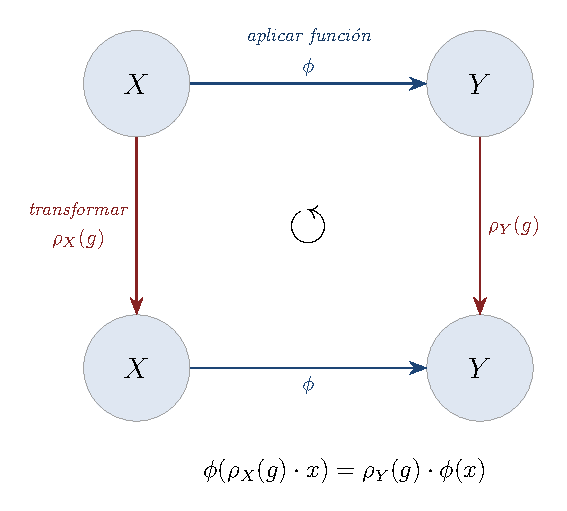
\includegraphics[width=0.65\textwidth]{images/equivariance_diagram.pdf}
\caption[Diagrama conmutativo de equivarianza]{Diagrama conmutativo de equivarianza. Una función $\phi: X \to Y$ es $G$-equivariante si el diagrama conmuta: aplicar primero la transformación $\rho_X(g)$ y luego $\phi$ produce el mismo resultado que aplicar primero $\phi$ y luego $\rho_Y(g)$.}
\label{fig:equivariance_diagram}
\end{figure}

Las \gls{ANN} tradicionales carecen de equivarianza por diseño. Para aproximar invarianza, requieren \textit{aumento de datos} (\autoref{def:data_augmentation}) con todas las transformaciones del grupo $G$, incrementando el tamaño del conjunto de entrenamiento por un factor $|G|$ sin garantía de generalización. El \gls{GDL} resuelve este problema incorporando simetrías directamente en la arquitectura, propagando equivarianza a través de todas las capas.

\begin{theorem}[Composición de Capas Equivariantes]\label{theorem:equivariant_composition}
Si $f: X \rightarrow Y$ y $g: Y \rightarrow Z$ son funciones equivariantes con respecto a las transformaciones $T_X$, $T_Y$ y $T_Z$ en los espacios $X$, $Y$ y $Z$ respectivamente, entonces su composición $g \circ f: X \rightarrow Z$ también es equivariante.
\end{theorem}

\begin{proof}
Sea $h \in G$ arbitrario y $x \in X$. Por la $G$-equivarianza de $f$:
\[
(g \circ f)(T_X(h) \cdot x) = g(f(T_X(h) \cdot x)) = g(T_Y(h) \cdot f(x))
\]
Por la $G$-equivarianza de $g$:
\[
= T_Z(h) \cdot g(f(x)) = T_Z(h) \cdot (g \circ f)(x)
\]
Por tanto, $g \circ f$ es $G$-equivariante.
\end{proof}

Este teorema garantiza que las redes profundas construidas mediante composición de capas equivariantes mantienen la equivarianza extremo a extremo, una propiedad fundamental para el diseño de arquitecturas geométricas.

\subsubsection{Teorema de Aproximación Universal Equivariante}\label{sec:teorema_equivariante}

El siguiente resultado, demostrado por \citet{yarotsky2022} y \citet{kondor2018generalizationconvolutionalneural}, extiende el teorema de aproximación universal clásico al caso equivariante:

\begin{theorem}[Aproximación Universal Equivariante]\label{theorem:universal_approximation_equivariant}
Sea $G$ un grupo compacto (\autoref{def:grupo_compacto}) que actúa continuamente sobre espacios métricos compactos $X$ e $Y$, y sea $\mathcal{F}^G(X,Y)$ el espacio de todas las funciones continuas $G$-equivariantes $f: X \rightarrow Y$. Entonces, para cualquier función $f \in \mathcal{F}^G(X,Y)$ y cualquier $\epsilon > 0$, existe una red neuronal $G$-equivariante $\mathcal{N}$ tal que:
\begin{equation}
\sup_{x \in X} d_Y(f(x), \mathcal{N}(x)) < \epsilon
\label{eq:universal_approximation_equivariant}
\end{equation}
donde $d_Y$ es la métrica en $Y$.
\end{theorem}

\begin{proof}
La demostración procede en cuatro pasos, siguiendo las ideas de \citet{yarotsky2022}.

\textbf{Paso 1: Aproximación no equivariante.}
Por el teorema de aproximación universal clásico (\autoref{thm:aproximacion_universal}), para cualquier función continua $f: X \to Y$ y $\epsilon > 0$, existe una red neuronal $\tilde{f}: X \to Y$ tal que $\sup_{x \in X} d_Y(f(x), \tilde{f}(x)) < \epsilon$.

\textbf{Paso 2: Construcción del promediado equivariante.}
Definimos el \textit{operador de Reynolds} mediante el promediado sobre el grupo:
\[
\overline{f}(x) = \int_G \rho_Y(g^{-1}) \tilde{f}(g \cdot x) \, d\mu(g)
\]
donde $\rho_Y: G \to GL(Y)$ es la representación de $G$ en $Y$ (\autoref{def:equivariance_gdl}), y $\mu$ es la medida de Haar normalizada sobre $G$ (\autoref{def:medida_haar_gdl}).

\textbf{Paso 3: Verificación de la equivarianza.}
Verificamos que $\overline{f}$ es $G$-equivariante. Para cualquier $h \in G$:
\begin{align*}
\overline{f}(h \cdot x) &= \int_G \rho_Y(g^{-1}) \tilde{f}(g \cdot (h \cdot x)) \, d\mu(g) \\
&= \int_G \rho_Y(g^{-1}) \tilde{f}((gh) \cdot x) \, d\mu(g)
\end{align*}
Realizando el cambio de variables $g' = gh$, y usando la invarianza de la medida de Haar ($d\mu(g) = d\mu(g')$):
\begin{align*}
&= \int_G \rho_Y((g'h^{-1})^{-1}) \tilde{f}(g' \cdot x) \, d\mu(g') \\
&= \int_G \rho_Y(h)\rho_Y(g'^{-1}) \tilde{f}(g' \cdot x) \, d\mu(g') \\
&= \rho_Y(h) \int_G \rho_Y(g'^{-1}) \tilde{f}(g' \cdot x) \, d\mu(g') = \rho_Y(h) \overline{f}(x)
\end{align*}
Por tanto, $\overline{f}$ es $G$-equivariante según la \autoref{def:equivariance_gdl}.

\textbf{Paso 4: Control del error de aproximación.}
Sea $f$ la función $G$-equivariante objetivo. Por la linealidad de la integral y la equivarianza de $f$:
\begin{align*}
d_Y(\overline{\tilde{f}}(x), f(x)) &\leq \int_G d_Y(\rho_Y(g^{-1}) \tilde{f}(g \cdot x), \rho_Y(g^{-1}) f(g \cdot x)) \, d\mu(g)
\end{align*}
Para grupos compactos, las representaciones pueden elegirse unitarias, por lo que $\rho_Y(g^{-1})$ preserva distancias:
\[
\leq \int_G d_Y(\tilde{f}(g \cdot x), f(g \cdot x)) \, d\mu(g) \leq \sup_{x' \in X} d_Y(\tilde{f}(x'), f(x')) < \epsilon
\]
La última desigualdad usa que la acción de $G$ sobre el compacto $X$ preserva la compacidad.
\end{proof}

\textbf{Implicaciones para el diseño de arquitecturas.} Este teorema es crucial porque demuestra que las restricciones de equivarianza no limitan la capacidad expresiva de las redes neuronales. Específicamente:

\begin{itemize}
    \item Las redes $G$-equivariantes pueden aproximar cualquier función $G$-equivariante continua
    \item No es necesario sacrificar poder expresivo por equivarianza
    \item La equivarianza actúa como un sesgo inductivo que reduce el espacio de funciones sin perder capacidad de aproximación en el subespacio relevante
\end{itemize}

\begin{example}[CNNs como caso especial]
Para el grupo de traslaciones $G = \mathbb{Z}^2$ actuando sobre imágenes discretas, este teorema garantiza que las \glspl{CNN} (que son equivariantes a traslaciones, véase \autoref{ch:cnn}) pueden aproximar cualquier función continua que sea invariante o equivariante a traslaciones. Esto justifica teóricamente el éxito de las \glspl{CNN} en tareas de visión por computador.
\end{example}

\subsection{Espacios Homogéneos y Dominios Geométricos}\label{subsec:espacios_homogeneos}

Hasta ahora hemos estudiado la equivarianza como propiedad algebraica de funciones entre espacios de señales. Sin embargo, muchos dominios de datos importantes en \gls{GDL} (la esfera $S^2$, el espacio proyectivo, las variedades de Grassmann) comparten una estructura geométrica común: pueden expresarse como cocientes $G/H$ de un grupo de Lie por un subgrupo cerrado. Esta observación permite unificar el diseño de arquitecturas equivariantes para dominios aparentemente distintos bajo un mismo marco teórico.

\begin{definition}[Espacio Homogéneo]\label{def:espacio_homogeneo}
Sea $G$ un grupo de Lie y $H$ un subgrupo cerrado. El \textit{espacio homogéneo} $G/H$ es el conjunto de clases laterales izquierdas:
\begin{equation}
G/H = \{gH : g \in G\}
\end{equation}
El grupo $G$ actúa transitivamente sobre $G/H$ mediante $g' \cdot (gH) = (g'g)H$.
\end{definition}

\subsubsection{Fundamentos teóricos}

Para formalizar la estructura de cociente $G/H$, necesitamos dos conceptos de la teoría de acciones de grupo: la \textit{órbita} de un elemento (todos los puntos alcanzables por la acción) y su \textit{estabilizador} (el subgrupo que lo deja fijo). El teorema órbita-estabilizador conectará ambas nociones y justificará por qué todo espacio homogéneo admite una representación como cociente.

\begin{definition}[Órbita]\label{def:orbita}
Sea $G$ un grupo actuando sobre un conjunto $X$. Para cualquier elemento $x \in X$, la \textit{órbita} de $x$ bajo la acción de $G$ es:
\begin{equation}
\text{Orb}(x) = \{g \cdot x : g \in G\}
\end{equation}
Es decir, el conjunto de todos los elementos de $X$ que pueden alcanzarse aplicando elementos de $G$ a $x$.
\end{definition}

\begin{definition}[Subgrupo Estabilizador]\label{def:estabilizador}
Sea $G$ un grupo actuando sobre un conjunto $X$. Para cualquier elemento $x \in X$, el \textit{subgrupo estabilizador} (o isotrópico) de $x$ es:
\begin{equation}
\text{Stab}(x) = \{g \in G : g \cdot x = x\}
\end{equation}
Es decir, el subgrupo de todos los elementos de $G$ que dejan $x$ invariante.
\end{definition}

La relación fundamental entre estos conceptos está capturada por el teorema órbita-estabilizador, que es central para entender la estructura de espacios homogéneos:

\begin{theorem}[Teorema Órbita-Estabilizador]\label{thm:orbita_estabilizador}
Sea $G$ un grupo actuando sobre un conjunto $X$, y sea $x \in X$. Entonces existe un isomorfismo natural:
\begin{equation}
G/\text{Stab}(x) \cong \text{Orb}(x)
\end{equation}
\end{theorem}

\begin{proof}
Construimos una biyección directa $\psi: G/\mathrm{Stab}(x) \to \mathrm{Orb}(x)$ definida por $\psi(g\,\mathrm{Stab}(x)) = g \cdot x$.

\textbf{Buena definición.} Si $g\,\mathrm{Stab}(x) = h\,\mathrm{Stab}(x)$, entonces $h^{-1}g \in \mathrm{Stab}(x)$, es decir, $(h^{-1}g) \cdot x = x$. Luego $g \cdot x = h \cdot ((h^{-1}g) \cdot x) = h \cdot x$, y $\psi$ está bien definida.

\textbf{Inyectividad.} Si $\psi(g\,\mathrm{Stab}(x)) = \psi(h\,\mathrm{Stab}(x))$, entonces $g \cdot x = h \cdot x$, de donde $(h^{-1}g) \cdot x = x$ y $h^{-1}g \in \mathrm{Stab}(x)$. Por tanto $g\,\mathrm{Stab}(x) = h\,\mathrm{Stab}(x)$.

\textbf{Sobreyectividad.} Todo $y \in \mathrm{Orb}(x)$ es, por definición, de la forma $y = g \cdot x$ para algún $g \in G$, luego $y = \psi(g\,\mathrm{Stab}(x))$.
\end{proof}

Este teorema es fundamental para \gls{GDL} porque establece que cualquier dominio geométrico que admita simetrías transitivas puede representarse como un espacio homogéneo $G/H$, donde $G$ es el grupo de simetrías y $H$ es el subgrupo que fija un punto de referencia.

\begin{figure}[htbp]
\centering
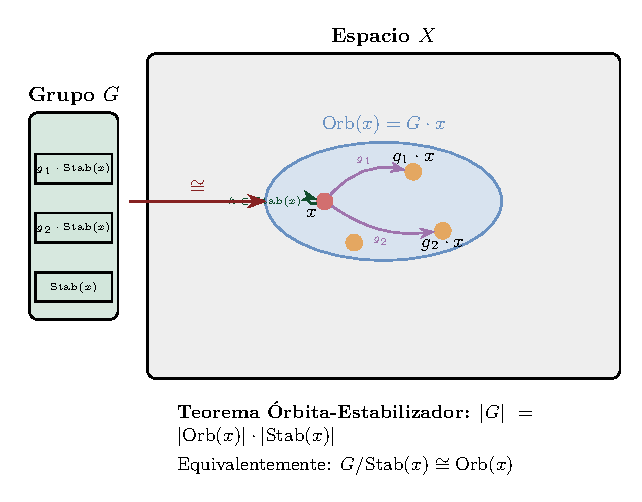
\includegraphics[width=0.7\textwidth]{images/orbit_stabilizer.pdf}
\caption[Teorema Órbita-Estabilizador]{Visualización del Teorema Órbita-Estabilizador. La órbita $\mathrm{Orb}(x)$ bajo la acción de $G$ es isomorfa al espacio cociente $G/\mathrm{Stab}(x)$: cada clase lateral $g\,\mathrm{Stab}(x)$ corresponde a exactamente un punto de la órbita.}
\label{fig:orbit_stabilizer}
\end{figure}

\begin{example}[Aplicación del Teorema en \gls{GDL}]\label{ex:aplicacion_teorema_gdl}
Consideremos la esfera $S^2$ como dominio para datos direccionales, con $G = SO(3)$ actuando por rotaciones.

\textbf{Identificación del cociente.}
\begin{itemize}
    \item \emph{Transitividad}: $SO(3)$ actúa transitivamente sobre $S^2$. En efecto, dados $\mathbf{x}, \mathbf{y} \in S^2$, cada uno puede completarse a una base ortonormal positiva de $\mathbb{R}^3$, y la rotación que envía una base a la otra satisface $R\mathbf{x} = \mathbf{y}$. Por tanto $\mathrm{Orb}(\mathbf{p}) = S^2$ para cualquier punto de referencia $\mathbf{p}$.

    \item \emph{Estabilizador}: Tomemos el polo norte $\mathbf{p} = (0,0,1)^{\!\top}$. Una rotación $R \in SO(3)$ fija $\mathbf{p}$ si y solo si su eje de rotación es el eje $z$, es decir, $R = R_z(\theta)$ para algún $\theta \in [0, 2\pi)$ (véase \autoref{ex:so3_rotaciones}). Estas rotaciones forman un subgrupo isomorfo a $SO(2)$, luego $\mathrm{Stab}(\mathbf{p}) \cong SO(2)$.

    \item \emph{Interpretación de las clases laterales}: Dos rotaciones $g_1, g_2 \in SO(3)$ producen el mismo punto sobre $S^2$ (es decir, $g_1 \cdot \mathbf{p} = g_2 \cdot \mathbf{p}$) si y solo si $g_1^{-1}g_2 \in SO(2)$, lo que significa que difieren por una rotación alrededor del eje que pasa por dicho punto. Cada clase lateral $gSO(2)$ corresponde a exactamente un punto de la esfera.
\end{itemize}
Aplicando el Teorema~\ref{thm:orbita_estabilizador} se obtiene
\begin{equation}\label{eq:esfera_cociente_ejemplo}
    S^2 \cong SO(3)/SO(2).
\end{equation}
La demostración rigurosa para $S^{n-1}$ en dimensión arbitraria se presenta en la Proposición~\ref{prop:esfera_cociente}.

\textbf{Interpretación para el procesamiento de señales.}
Una señal sobre la esfera $f\colon S^2 \to \mathbb{R}^C$ puede ``elevarse'' a una función sobre $SO(3)$ que es invariante a derecha por $SO(2)$: basta definir $\tilde{f}(g) = f(g \cdot \mathbf{p})$, de modo que $\tilde{f}(gh) = \tilde{f}(g)$ para todo $h \in SO(2)$. Como consecuencia, la convolución equivariante sobre $S^2$ debe definirse como correlación sobre el grupo completo $SO(3)$, en lugar de como convolución en una proyección plana (que introduciría distorsiones). De esta forma, la primera capa convolucional transforma señales de $S^2$ en funciones sobre $SO(3)$, y las capas sucesivas operan directamente sobre $SO(3)$. Los detalles técnicos de esta construcción se desarrollan en la \autoref{subsec:spherical_cnns_so3}.

\textbf{Aplicaciones.}
\begin{enumerate}
    \item \emph{Datos climáticos y geofísicos}: las señales sobre la superficie terrestre (temperatura, presión, viento) son funciones sobre $S^2$. La equivarianza bajo $SO(3)$ garantiza que las predicciones no dependan de la elección de coordenadas geográficas \citep{cohen2018sphericalcnns}.

    \item \emph{Visión omnidireccional}: las imágenes de $360^\circ$ se representan naturalmente como señales sobre $S^2$. Procesar estas señales directamente sobre la esfera evita las distorsiones inherentes a las proyecciones equirrectangulares o cúbicas que emplean las \glspl{CNN} planares.

    \item \emph{Orientaciones moleculares}: las superficies moleculares carecen de una orientación preferente. Utilizar arquitecturas $SO(3)$-equivariantes garantiza representaciones físicamente significativas, independientes de la orientación arbitraria en que se presente la molécula.
\end{enumerate}

\textbf{Metodología general.}
Este ejemplo ilustra un patrón sistemático para diseñar arquitecturas de \gls{GDL}: (1)~identificar el dominio $\Omega$ de los datos; (2)~determinar el grupo de simetrías $G$ relevante; (3)~calcular el estabilizador $H$ de un punto de referencia; (4)~reconocer $\Omega \cong G/H$ mediante el Teorema Órbita-Estabilizador; y (5)~construir la arquitectura equivariante utilizando el análisis armónico de $G$ (Teorema de Peter-Weyl~\ref{thm:peter_weyl}). Las Proposiciones~\ref{prop:esfera_cociente}--\ref{prop:grassmann_stiefel_cociente} aplican esta metodología sistemáticamente a los dominios fundamentales del \gls{GDL}.
\end{example}

\paragraph{Propiedades geométricas fundamentales}

Los espacios homogéneos poseen propiedades geométricas distintivas que los hacen especialmente apropiados para el Deep Learning:

\begin{proposition}[Transitividad y Conectividad]\label{prop:transitividad_espacios_homogeneos}
Sea $G/H$ un espacio homogéneo. Entonces:
\begin{enumerate}
    \item $G$ actúa transitivamente sobre $G/H$: dados $g_1H, g_2H \in G/H$, existe $g \in G$ tal que $g \cdot (g_1H) = g_2H$
    \item Si $G$ es conexo, entonces $G/H$ es conexo
    \item La acción de $G$ preserva cualquier métrica $G$-invariante sobre $G/H$
\end{enumerate}
\end{proposition}

\begin{proof}
\leavevmode
\begin{enumerate}
    \item \textbf{Transitividad.} Dados $g_1H, g_2H \in G/H$, sea $g = g_2 g_1^{-1} \in G$. Entonces:
    \[
    g \cdot (g_1H) = (g_2 g_1^{-1}) g_1 H = g_2 H
    \]

    \item \textbf{Conectividad.} La proyección canónica $\pi: G \to G/H$, $\pi(g) = gH$, es continua por definición de la topología cociente y sobreyectiva por definición. Como $G$ es conexo, $G/H = \pi(G)$ es conexo (imagen continua de un espacio conexo es conexa).

    \item \textbf{Preservación de métrica.} Sea $g$ una métrica $G$-invariante sobre $G/H$ (\autoref{def:metrica_invariante}). Para todo $\gamma \in G$, la aplicación $L_\gamma: p \mapsto \gamma \cdot p$ satisface por definición de $G$-invarianza:
    \[
    g_p(u, v) = g_{\gamma \cdot p}(d(L_\gamma)_p\, u,\; d(L_\gamma)_p\, v)
    \]
    para todo $p \in G/H$ y $u, v \in T_p(G/H)$. Esto significa que $L_\gamma^* g = g$, es decir, $L_\gamma$ es una isometría. \qedhere
\end{enumerate}
\end{proof}

\begin{definition}[Métrica Invariante]\label{def:metrica_invariante}
Una métrica riemanniana $g$ sobre un espacio homogéneo $G/H$ es \textit{$G$-invariante} si para todo $\gamma \in G$ y vectores tangentes $u, v \in T_p(G/H)$:
\begin{equation}
g_p(u, v) = g_{\gamma \cdot p}(d\gamma_p u, d\gamma_p v)
\end{equation}
donde $d\gamma_p$ denota la diferencial de la acción de $\gamma$ en el punto $p$.
\end{definition}

\paragraph{Correspondencia entre geometría y equivarianza}

La teoría de espacios homogéneos establece una conexión fundamental entre la estructura geométrica de los dominios de datos y las propiedades de equivarianza de las funciones definidas sobre ellos.

\begin{theorem}[Determinación de operadores equivariantes por el punto base]\label{thm:correspondencia_geometria_equivarianza}
Sea $\mathcal{M} = G/H$ un espacio homogéneo y sean $\rho_1, \rho_2$ representaciones de $G$ en espacios vectoriales $V_1, V_2$. Sea $\mathcal{F}(\mathcal{M}, V_i) = \{f: \mathcal{M} \to V_i\}$ el espacio de funciones sobre $\mathcal{M}$ con valores en $V_i$, con la acción regular a izquierda $(L_g f)(x) = \rho_i(g)\, f(g^{-1} \cdot x)$. Todo operador $G$-equivariante $\Phi: \mathcal{F}(\mathcal{M}, V_1) \to \mathcal{F}(\mathcal{M}, V_2)$ (es decir, $\Phi \circ L_g = L_g \circ \Phi$ para todo $g \in G$) está completamente determinado por sus valores en el punto base $o = eH$: si $\Phi_1$ y $\Phi_2$ son $G$-equivariantes y $(\Phi_1 f)(o) = (\Phi_2 f)(o)$ para toda $f$, entonces $\Phi_1 = \Phi_2$.
\end{theorem}

\begin{proof}
Sea $x \in \mathcal{M}$ un punto arbitrario. Como $G$ actúa transitivamente sobre $G/H$, existe $g \in G$ con $g \cdot o = x$. Para cualquier $f \in \mathcal{F}(\mathcal{M}, V_1)$, la $G$-equivarianza da:
\[
(\Phi f)(x) = (\Phi f)(g \cdot o) = \rho_2(g)\,(\Phi f)(g^{-1} \cdot (g \cdot o)) \quad \text{(evaluando } L_{g^{-1}}(\Phi f) \text{ en } o\text{)}
\]
Más precisamente, por equivarianza $L_g(\Phi f) = \Phi(L_g f)$, de donde:
\[
(\Phi f)(x) = (L_{g^{-1}}^{-1}(\Phi f))(o) = \rho_2(g)\,(\Phi(L_{g^{-1}} f))(o)
\]
puesto que $(L_{g^{-1}} h)(o) = \rho_2(g^{-1})\,h(g \cdot o) = \rho_2(g^{-1})\,h(x)$, lo que implica $h(x) = \rho_2(g)\,(L_{g^{-1}} h)(o)$. Así, $(\Phi f)(x) = \rho_2(g)\,(\Phi(L_{g^{-1}} f))(o)$, y el valor de $\Phi f$ en cualquier punto $x$ queda determinado por la evaluación de $\Phi$ en el punto base $o$.
\end{proof}

\begin{corollary}[Operadores Lineales Equivariantes]\label{cor:operadores_equivariantes}
Sea $G$ un grupo de Lie compacto actuando transitivamente sobre sí mismo por traslación izquierda, y sea $\Phi: L^2(G) \to L^2(G)$ un operador lineal continuo $G$-equivariante (es decir, $\Phi \circ L_g = L_g \circ \Phi$ para todo $g \in G$). Entonces $\Phi$ es un operador de convolución generalizada sobre $G$.
\end{corollary}

\begin{proof}
Por el \autoref{thm:correspondencia_geometria_equivarianza}, $\Phi$ está determinado por sus valores en la identidad $e \in G$. La equivarianza y linealidad implican que $\Phi$ admite una representación como operador integral con kernel $k$:
\[
(\Phi f)(g) = \int_{G} k(g, g') f(g')\, d\mu(g')
\]
donde $\mu$ es la medida de Haar normalizada. La condición de equivarianza $\Phi(L_h f) = L_h(\Phi f)$ implica, por un cálculo directo con cambio de variable, que $k(hg, hg') = k(g, g')$ para todo $h \in G$. Tomando $h = g^{-1}$, obtenemos $k(g, g') = k(e, g^{-1}g') = \kappa(g^{-1}g')$ para la función $\kappa = k(e, \cdot): G \to \mathbb{R}$. El operador $\Phi$ toma entonces la forma de convolución:
\[
(\Phi f)(g) = \int_{G} \kappa(g^{-1}g') f(g')\, d\mu(g') = (\kappa * f)(g) \qedhere
\]
\end{proof}

Este resultado justifica matemáticamente por qué las convoluciones son la operación natural en arquitecturas equivariantes: son precisamente los operadores lineales que respetan la estructura de simetría del dominio.

\textbf{Consecuencias para \gls{GDL}.}
\begin{enumerate}
    \item \textbf{Principio de invarianza necesaria}: Solo las simetrías genuinas del problema deben ser incorporadas en la arquitectura. Simetrías artificiales pueden degradar el rendimiento.

    \item \textbf{Jerarquía de equivarianzas}: En espacios homogéneos con múltiples niveles de simetría, las arquitecturas pueden implementar equivarianza aproximada en capas tempranas e invarianza exacta en capas finales.

    \item \textbf{Transferibilidad geométrica}: Modelos entrenados en un espacio homogéneo $G/H$ pueden transferirse a otros espacios homogéneos $G/H'$ si existe un homomorfismo natural entre los estabilizadores $H$ y $H'$.
\end{enumerate}

\paragraph{Representaciones fundamentales como cocientes}

El Teorema Órbita-Estabilizador~\ref{thm:orbita_estabilizador} y el \autoref{ex:aplicacion_teorema_gdl} mostraron cómo $S^2 \cong SO(3)/SO(2)$. Aplicamos ahora la misma técnica sistemáticamente a los espacios no euclidianos introducidos en la \autoref{subsec:espacios_no_euclidianos}, justificando rigurosamente cada representación $G/H$.

\begin{proposition}[Esfera como Espacio Homogéneo]\label{prop:esfera_cociente}
La esfera $S^{n-1}$ (\autoref{def:esfera_n}) es un espacio homogéneo:
\[
S^{n-1} \cong SO(n)/SO(n-1).
\]
\end{proposition}

\begin{proof}
Sea $\mathbf{e}_n = (0,\ldots,0,1) \in S^{n-1}$ el polo norte. El grupo $SO(n)$ (\autoref{def:grupo_so_n}) actúa sobre $S^{n-1}$ por multiplicación matricial: si $R \in SO(n)$ y $\mathbf{x} \in S^{n-1}$, entonces $\|R\mathbf{x}\| = \|\mathbf{x}\| = 1$, por lo que $R\mathbf{x} \in S^{n-1}$.

\textit{Transitividad.} Dado $\mathbf{x} \in S^{n-1}$, completamos $\mathbf{x}$ a una base ortonormal positiva $\{\mathbf{v}_1, \ldots, \mathbf{v}_{n-1}, \mathbf{x}\}$ de $\mathbb{R}^n$ mediante el proceso de Gram-Schmidt. La matriz $R = [\mathbf{v}_1 \mid \cdots \mid \mathbf{v}_{n-1} \mid \mathbf{x}]$ satisface $R \in SO(n)$ y $R\mathbf{e}_n = \mathbf{x}$.

\textit{Estabilizador.} Si $R\mathbf{e}_n = \mathbf{e}_n$, la última columna de $R$ es $\mathbf{e}_n$ y la ortogonalidad fuerza que $R$ tenga la forma:
\[
R = \begin{pmatrix} A & 0 \\ 0 & 1 \end{pmatrix}, \quad A \in SO(n-1).
\]
Luego $\mathrm{Stab}(\mathbf{e}_n) \cong SO(n-1)$.

Por el Teorema Órbita-Estabilizador~\ref{thm:orbita_estabilizador}, $S^{n-1} = \mathrm{Orb}(\mathbf{e}_n) \cong SO(n)/SO(n-1)$. Este resultado generaliza el \autoref{ex:aplicacion_teorema_gdl} de $S^2 \cong SO(3)/SO(2)$ a dimensión arbitraria.
\end{proof}

La compacidad de $SO(n)$ refleja algebraicamente la curvatura positiva constante $K=+1$ de la esfera; este espacio homogéneo es fundamental para datos direccionales, visión omnidireccional y orientaciones moleculares.

\begin{proposition}[Espacio Euclidiano como Espacio Homogéneo]\label{prop:euclidiano_cociente}
El espacio euclidiano es un espacio homogéneo:
\[
\mathbb{R}^n \cong E(n)/O(n) \cong SE(n)/SO(n).
\]
\end{proposition}

\begin{proof}
El grupo euclidiano $E(n) = \mathbb{R}^n \rtimes O(n)$ (\autoref{def:grupo_e_n}) actúa sobre $\mathbb{R}^n$ por $(t, R) \cdot x = Rx + t$.

\textit{Transitividad.} Para todo $x \in \mathbb{R}^n$, $(x, I_n) \cdot \mathbf{0} = x$, así que la órbita del origen es todo $\mathbb{R}^n$.

\textit{Estabilizador.} Si $(t, R) \cdot \mathbf{0} = t = \mathbf{0}$, entonces $t = \mathbf{0}$ y $R$ es arbitrario en $O(n)$. Luego $\mathrm{Stab}(\mathbf{0}) \cong O(n)$.

El Teorema Órbita-Estabilizador~\ref{thm:orbita_estabilizador} da $\mathbb{R}^n \cong E(n)/O(n)$. Restringiendo al grupo euclidiano especial $SE(n) = \mathbb{R}^n \rtimes SO(n)$ (\autoref{def:grupo_se_n}), que también actúa transitivamente, se obtiene análogamente $\mathbb{R}^n \cong SE(n)/SO(n)$.
\end{proof}

La curvatura $K=0$ se refleja en que la componente traslacional de $E(n)$ es abeliana; este es el caso base de las \glspl{CNN} clásicas, donde la equivarianza traslacional se implementa mediante convoluciones estándar.

\begin{proposition}[Espacio Proyectivo como Espacio Homogéneo]\label{prop:proyectivo_cociente}
El espacio proyectivo real (\autoref{def:espacio_proyectivo}) es un espacio homogéneo:
\[
\mathbb{RP}^{n-1} \cong O(n)/(O(n-1) \times \mathbb{Z}_2).
\]
\end{proposition}

\begin{proof}
El grupo ortogonal $O(n)$ (\autoref{def:grupo_o_n}) actúa sobre el conjunto de líneas por el origen en $\mathbb{R}^n$ mediante $R \cdot [\mathbf{x}] = [R\mathbf{x}]$. La acción está bien definida: si $[\mathbf{x}] = [\mathbf{y}]$, entonces $\mathbf{y} = \lambda \mathbf{x}$ con $\lambda \neq 0$, y $[R\mathbf{y}] = [\lambda R\mathbf{x}] = [R\mathbf{x}]$.

\textit{Transitividad.} Toda línea por el origen contiene un vector unitario. Como $O(n)$ actúa transitivamente sobre $S^{n-1}$ (pues tanto rotaciones como reflexiones preservan la norma), actúa transitivamente sobre las líneas.

\textit{Estabilizador.} La línea $[\mathbf{e}_n]$ es fijada por $R$ si y solo si $R\mathbf{e}_n = \pm\mathbf{e}_n$. En ambos casos, la ortogonalidad fuerza:
\[
R = \begin{pmatrix} A & 0 \\ 0 & \pm 1 \end{pmatrix}, \quad A \in O(n-1).
\]
Luego $\mathrm{Stab}([\mathbf{e}_n]) \cong O(n-1) \times \mathbb{Z}_2$, y el resultado sigue del Teorema Órbita-Estabilizador~\ref{thm:orbita_estabilizador}.
\end{proof}

El factor $\mathbb{Z}_2$ en el estabilizador refleja la identificación antipodal que define el espacio proyectivo; la curvatura se hereda de $S^{n-1}$ vía el recubrimiento doble $S^{n-1} \to \mathbb{RP}^{n-1}$.

\begin{proposition}[Espacio Hiperbólico como Espacio Homogéneo]\label{prop:hiperbolico_cociente}
El espacio hiperbólico (\autoref{def:espacio_hiperbolico}) es un espacio homogéneo:
\[
\mathbb{H}^n \cong SO^+(n,1)/SO(n).
\]
\end{proposition}

\begin{proof}
Consideramos $\mathbb{H}^n$ en el modelo del hiperboloide: $\mathbb{H}^n = \{x \in \mathbb{R}^{n+1} : x_0^2 - x_1^2 - \cdots - x_n^2 = 1, \; x_0 > 0\}$. El grupo $SO^+(n,1)$, la componente conexa de la identidad del grupo de Lorentz, preserva la forma cuadrática de Lorentz $\langle x, y \rangle_{n,1} = x_0 y_0 - \sum_{i=1}^n x_i y_i$ y la condición $x_0 > 0$.

\textit{Transitividad.} Dados dos puntos $p, q \in \mathbb{H}^n$, la composición de un boost de Lorentz (hiperbólico) que lleva $p$ al punto base $\mathbf{e}_0 = (1,0,\ldots,0)$, seguida de otro boost que lleva $\mathbf{e}_0$ a $q$, proporciona un elemento de $SO^+(n,1)$ que envía $p$ a $q$.

\textit{Estabilizador.} Si $g \in SO^+(n,1)$ fija $\mathbf{e}_0 = (1,0,\ldots,0)$, entonces $g$ preserva el complemento ortogonal de $\mathbf{e}_0$ respecto a la forma de Lorentz, que es el subespacio espacial $\{0\} \times \mathbb{R}^n$, donde la forma de Lorentz restringe a $-\sum_{i=1}^n x_i^2$. Por tanto, $g$ actúa como una rotación en las coordenadas espaciales, luego $\mathrm{Stab}(\mathbf{e}_0) \cong SO(n)$.

Por el Teorema Órbita-Estabilizador~\ref{thm:orbita_estabilizador}, $\mathbb{H}^n \cong SO^+(n,1)/SO(n)$.
\end{proof}

A diferencia del caso esférico, $SO^+(n,1)$ es no compacto, lo cual refleja algebraicamente la curvatura negativa $K=-1$ y el crecimiento exponencial del volumen de bolas en $\mathbb{H}^n$.

\begin{proposition}[Variedades de Grassmann y Stiefel como Espacios Homogéneos]\label{prop:grassmann_stiefel_cociente}
Las variedades de Grassmann y Stiefel (\autoref{def:variedad_grassmann}) son espacios homogéneos:
\[
Gr(k,n) \cong O(n)/(O(k) \times O(n-k)), \qquad St(k,n) \cong O(n)/O(n-k).
\]
\end{proposition}

\begin{proof}
\textit{Grassmann.} El grupo $O(n)$ actúa sobre el conjunto de subespacios $k$-dimensionales de $\mathbb{R}^n$ por $R \cdot V = \{Rv : v \in V\}$.

La acción es transitiva: dado un subespacio $V$ de dimensión $k$, elegimos una base ortonormal $\{v_1,\ldots,v_k\}$ de $V$ y la completamos a una base ortonormal $\{v_1,\ldots,v_n\}$ de $\mathbb{R}^n$. La matriz $R = [v_1 \mid \cdots \mid v_n] \in O(n)$ satisface $R \cdot \mathrm{span}(\mathbf{e}_1,\ldots,\mathbf{e}_k) = V$.

El estabilizador de $V_0 = \mathrm{span}(\mathbf{e}_1,\ldots,\mathbf{e}_k)$ consiste en las matrices $R \in O(n)$ que preservan $V_0$ y su complemento ortogonal $V_0^\perp$. Estas tienen la forma diagonal por bloques:
\[
R = \begin{pmatrix} A & 0 \\ 0 & B \end{pmatrix}, \quad A \in O(k), \; B \in O(n-k).
\]
Luego $\mathrm{Stab}(V_0) \cong O(k) \times O(n-k)$ y $Gr(k,n) \cong O(n)/(O(k) \times O(n-k))$.

\textit{Stiefel.} La variedad de Stiefel $St(k,n)$ es el espacio de $k$-marcos ortonormales en $\mathbb{R}^n$. Tomando como punto base el marco canónico $(\mathbf{e}_1,\ldots,\mathbf{e}_k)$, el estabilizador consiste en las matrices de $O(n)$ que fijan los primeros $k$ vectores canónicos, es decir, matrices de la forma $\mathrm{diag}(I_k, B)$ con $B \in O(n-k)$. Luego $St(k,n) \cong O(n)/O(n-k)$.
\end{proof}

El estabilizador $O(k) \times O(n{-}k)$ separa las rotaciones dentro del subespacio de las del complemento ortogonal, reflejando la métrica de ángulos principales. La proyección natural $\pi\colon St(k,n) \to Gr(k,n)$ olvida la base específica y retiene solo el subespacio generado.

En las proposiciones anteriores, el par $(G, H)$ codifica toda la información geométrica: $G$ captura las simetrías globales y $H$ la simetría local en un punto, determinando curvatura, compacidad y crecimiento de volumen. Completamos ahora el panorama con dos familias de espacios homogéneos cuyos cocientes involucran grupos unitarios y lineales generales.

\paragraph{Espacios Complejos}

\begin{definition}[Espacio Proyectivo Complejo]\label{def:cp_homogeneo}
El \textit{espacio proyectivo complejo} $\mathbb{CP}^{n-1}$ es el espacio de líneas complejas en $\mathbb{C}^n$:
\begin{equation}
\mathbb{CP}^{n-1} = SU(n)/S(U(n-1) \times U(1)) = U(n)/(U(n-1) \times U(1))
\end{equation}
Es una variedad Kähler compacta, fundamental en mecánica cuántica (espacio de estados puros) y procesamiento de señales complejas.
\end{definition}

\paragraph{Espacios de Matrices}

\begin{definition}[Variedad de Matrices Simétricas Definidas Positivas]\label{def:spd_homogeneo}
El espacio $\mathrm{Sym}^+(n)$ de matrices simétricas $n \times n$ definidas positivas es:
\begin{equation}
\mathrm{Sym}^+(n) = GL(n)/O(n)
\end{equation}
Equipado con la métrica afín-invariante, es un espacio simétrico de curvatura no positiva. Es fundamental en estadística geométrica para matrices de covarianza y tensores de difusión.
\end{definition}

\begin{remark}[Espacios homogéneos y arquitecturas de GDL]\label{rem:espacios_homogeneos_arquitecturas}
	La clasificación de espacios homogéneos tiene implicaciones directas para el diseño de arquitecturas neuronales en \gls{GDL}. La \autoref{tab:espacios_homogeneos_arquitecturas} resume las conexiones principales:

	\begin{table}[htbp]
	\centering
	\caption{Correspondencia entre espacios homogéneos, arquitecturas de GDL y aplicaciones.}
	\label{tab:espacios_homogeneos_arquitecturas}
	\footnotesize
	\begin{tabular}{@{}llll@{}}
		\toprule
		\textbf{Espacio} & \textbf{Cociente $G/H$} & \textbf{Arquitectura} & \textbf{Aplicación} \\
		\midrule
		$S^{n-1}$ & $SO(n)/SO(n{-}1)$ & \makecell[l]{Spherical CNN \\  \citealp{cohen2018sphericalcnns}} & Clima, datos planetarios \\
		$\mathbb{R}^n$ & $E(n)/O(n)$ & \makecell[l]{CNN clásica \\ \citealp{cohen2016groupequivariantconvolutional}} & Imágenes, señales \\
		$\mathbb{RP}^{n-1}$ & $O(n)/(O(n{-}1) \times \mathbb{Z}_2)$ & \makecell[l]{Projective CNN} & Ejes sin orientación \\
		$\mathbb{H}^n$ & $SO^+(n,1)/SO(n)$ & \makecell[l]{Hyperbolic NN \\  \citealp{nickel2017poincare}} & Grafos de conocimiento \\
		$SE(3)/SO(3)$ & $\cong \mathbb{R}^3$ & \makecell[l]{SE(3)-equivariant \\  \citealp{fuchs2020se3transformers}} & Moléculas, proteínas \\
		$Gr(k,n)$ & $O(n)/(O(k) \times O(n{-}k))$ & \makecell[l]{Grassmann NN \\ \scriptsize \citealp{huang2017grassmann}} & Subspace clustering \\
		$\mathbb{CP}^{n-1}$ & $U(n)/(U(n{-}1) \times U(1))$ & \makecell[l]{Complex NN} & Mecánica cuántica \\
		$\mathrm{Sym}^+(n)$ & $GL(n)/O(n)$ & \makecell[l]{SPD-Net \\  \citealp{huang2017spd}} & Covarianzas, EEG \\
		\bottomrule
	\end{tabular}
	\end{table}

	Más allá de la clasificación, la naturaleza algebraica de $G$ determina la estrategia computacional. Cuando $G$ es compacto (como $SO(n)$ para la esfera), el Teorema de Peter-Weyl~\ref{thm:peter_weyl} proporciona una base completa de representaciones irreducibles que permite construir filtros equivariantes en el dominio espectral. Cuando $G$ es no compacto (como $SO^+(n,1)$ para el espacio hiperbólico), esta descomposición armónica no está disponible directamente, y se recurre a operaciones en el espacio tangente mediante los mapas exponencial y logarítmico.

	Esta correspondencia ilustra un principio fundamental del \gls{GDL}: la elección del espacio homogéneo determina el grupo de simetría $G$ y el estabilizador $H$, lo cual a su vez dicta la estructura de las representaciones equivariantes disponibles.
\end{remark}


\section{Grafos: La Discretización de Geometrías}\label{sec:grafos_discretizacion}

Las redes neuronales operan sobre estructuras finitas y discretas, pero los datos del mundo real a menudo residen en variedades continuas: superficies curvas, el espacio euclidiano tridimensional, la esfera terrestre. Los grafos constituyen el puente natural entre ambos mundos. Mediante la construcción de \textbf{grafos de proximidad}, una variedad continua se aproxima por un conjunto finito de puntos conectados por aristas que codifican relaciones de vecindad, preservando propiedades topológicas y espectrales esenciales.

Esta aproximación tiene implicaciones profundas para el \gls{GDL}. Por un lado, justifica teóricamente el uso de \glspl{GNN} para datos que residen naturalmente en variedades (moléculas, nubes de puntos 3D, datos climáticos). Por otro lado, establece límites fundamentales: cualquier información geométrica de la estructura continua que no sea capturada por la discretización será inaccesible para las arquitecturas basadas en grafos.

\subsection{Grafos como Discretización de Variedades}\label{subsec:grafos_discretizacion_variedades}

Formalmente, la aproximación discreta de una variedad $\mathcal{M}$ se construye a partir de un muestreo finito de puntos y una regla de conectividad basada en distancias. Recordemos que las definiciones fundamentales de grafos (grafo, grafo dirigido y no dirigido, caminos y ciclos) fueron introducidas en la \autoref{sec:redes_grafos} del \autoref{ch:neural_networks}. Aquí extendemos estos conceptos al contexto geométrico, dotando a los grafos de pesos que codifican información métrica de la variedad subyacente.

\begin{definition}[Grafo ponderado]\label{def:grafo_ponderado}
	Un \textit{grafo ponderado} es un grafo $G = (V, E)$ equipado con una función de pesos $w: E \to \mathbb{R}$ que asigna un valor numérico a cada arista. Cuando el grafo es no dirigido, se requiere $w(u,v) = w(v,u)$.
\end{definition}

\begin{definition}[Vecindad]\label{def:vecindad_grafo}
	Para un vértice $v \in V$, la \textit{vecindad} de $v$ se define como:
	\[\mathcal{N}(v) = \{u \in V : (v,u) \in E\}\]
	es decir, el conjunto de todos los vértices que están directamente conectados a $v$ por una arista.
\end{definition}

\begin{definition}[Grafo de vecindad]\label{def:grafo_vecindad_epsilon}
	Dado un conjunto de puntos $\{x_i\}_{i=1}^n$ en una variedad $\mathcal{M}$, podemos construir un \textit{grafo de vecindad} $G = (V,E)$ donde:
	\begin{itemize}
		\item $V = \{x_1, \ldots, x_n\}$ (los vértices son los puntos muestreados)
		\item $(x_i, x_j) \in E$ si $d_\mathcal{M}(x_i, x_j) < \epsilon$ para algún umbral $\epsilon > 0$
	\end{itemize}
	donde $d_\mathcal{M}$ denota la distancia geodésica en $\mathcal{M}$ (\autoref{def:variedad_riemanniana}).
\end{definition}

Esta construcción simple tiene consecuencias profundas: si los puntos $\{x_i\}$ están suficientemente densos en $\mathcal{M}$ y el radio $\epsilon$ se elige apropiadamente, el grafo resultante $G$ captura propiedades topológicas y geométricas fundamentales de la variedad original.

\begin{figure}[htbp]
\centering
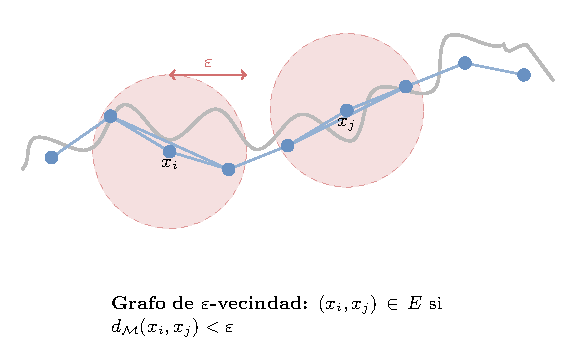
\includegraphics[width=0.7\textwidth]{images/epsilon_neighborhood_graph.pdf}
\caption[Grafo de $\epsilon$-vecindad]{Construcción de un grafo de $\epsilon$-vecindad. Los puntos muestreados de una variedad (izquierda) se conectan cuando su distancia es menor que $\epsilon$, formando un grafo que aproxima la estructura local de la variedad original (derecha).}
\label{fig:epsilon_neighborhood_graph}
\end{figure}

\paragraph{Grillas Regulares como Caso Especial}

Las grillas regulares sobre las cuales operan las \glspl{CNN} tradicionales son casos particulares de esta construcción general:

\begin{example}[Imagen 2D como grafo regular]\label{ex:imagen_grafo_grilla}
	Una imagen digital de dimensión $H \times W$ puede interpretarse como un grafo $G = (V,E)$ donde:
	\begin{itemize}
		\item $V = \{(i,j) : 1 \leq i \leq H, 1 \leq j \leq W\}$ (píxeles)
		\item $(i,j) \sim (i',j')$ si $|i-i'| + |j-j'| = 1$ (conectividad 4-vecindario)
	\end{itemize}

	Este grafo es una \textbf{discretización uniforme} del dominio continuo $[0,1] \times [0,1]$ con métrica euclidiana. La regularidad de la grilla se traduce en propiedades especiales:
	\begin{enumerate}
		\item Todos los nodos interiores tienen exactamente grado 4
		\item El grafo posee simetría traslacional discreta
		\item La distancia geodésica en el grafo aproxima la distancia $L^1$ en el dominio continuo
	\end{enumerate}
\end{example}

\begin{example}[Superficie 3D triangulada como grafo irregular]\label{ex:superficie_triangulada}
	Consideremos una superficie tridimensional $\mathcal{S} \subset \mathbb{R}^3$ (por ejemplo, un modelo 3D de un objeto). Una \textit{triangulación} de $\mathcal{S}$ produce un grafo $G = (V,E)$ donde:
	\begin{itemize}
		\item $V$ son los vértices de la triangulación
		\item $E$ son las aristas de los triángulos
	\end{itemize}

	A diferencia de las grillas regulares:
	\begin{enumerate}
		\item Los grados de los nodos son \textbf{heterogéneos} (típicamente entre 4 y 8 para mallas bien formadas)
		\item No existe simetría traslacional global
		\item La curvatura local de $\mathcal{S}$ se refleja en la densidad de vértices y la irregularidad del grafo
	\end{enumerate}

	Esta construcción es fundamental en gráficos por computadora, simulaciones físicas y análisis de formas 3D. Puesto que $\mathcal{S}$ es una superficie (2-variedad compacta), la existencia de tal triangulación está garantizada por el \autoref{thm:rado}. Las \glspl{GNN} sobre estas triangulaciones deben respetar la \textbf{equivarianza gauge} (véase \autoref{sec:gauges_invarianzas}): las predicciones no pueden depender de la orientación específica de la malla o de la parametrización elegida.
\end{example}

\paragraph{Símplices, Triangulaciones y Complejos Simpliciales}

Para formalizar las triangulaciones y sus generalizaciones, necesitamos definir con precisión los bloques constructivos fundamentales de la topología combinatoria.

\begin{definition}[$k$-símplice]\label{def:simplicio_gdl}
	Un \textit{$k$-símplice} $\sigma$ es la envolvente convexa (el conjunto de todas las combinaciones convexas) de $k+1$ puntos afínmente independientes $v_0, v_1, \ldots, v_k$ en $\mathbb{R}^n$:
	\[
		\sigma = [v_0, v_1, \ldots, v_k] = \left\{ \sum_{i=0}^k t_i v_i : \sum_{i=0}^k t_i = 1, \, t_i \geq 0 \right\}
	\]
	Los puntos $v_i$ se denominan \textit{vértices} del símplice, y $k$ es su \textit{dimensión}. Los casos fundamentales son: un 0-símplice es un punto, un 1-símplice una arista, un 2-símplice un triángulo, un 3-símplice un tetraedro, y así sucesivamente para dimensiones superiores.
\end{definition}

\begin{definition}[Cara de un símplice]\label{def:cara_simplicio_gdl}
	Una \textit{cara} de dimensión $j < k$ del $k$-símplice $\sigma = [v_0, v_1, \ldots, v_k]$ es cualquier símplice determinado por un subconjunto de $j+1$ vértices:
	\[
		\tau = [v_{i_0}, v_{i_1}, \ldots, v_{i_j}] \quad \text{con } \{i_0, i_1, \ldots, i_j\} \subseteq \{0, 1, \ldots, k\}
	\]
	Se denota $\tau \leq \sigma$ cuando $\tau$ es cara de $\sigma$.
\end{definition}

\begin{definition}[Complejo simplicial]\label{def:complejo_simplicial}
	Un \textit{complejo simplicial} $\mathcal{K}$ es una colección finita de símplices tal que:
	\begin{enumerate}
		\item Si $\sigma \in \mathcal{K}$ y $\tau \leq \sigma$, entonces $\tau \in \mathcal{K}$ (cerrado bajo caras)
		\item Si $\sigma, \tau \in \mathcal{K}$, entonces $\sigma \cap \tau$ es una cara de ambos (intersección bien definida)
	\end{enumerate}

	El \textit{1-esqueleto} de $\mathcal{K}$ es el grafo $G = (V,E)$ formado por los 0-símplices (vértices) y 1-símplices (aristas).
\end{definition}

\begin{figure}[htbp]
\centering
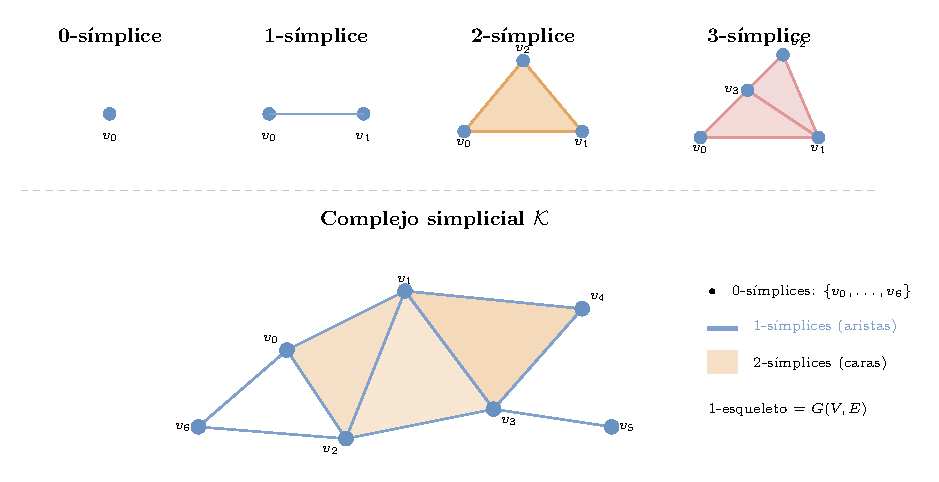
\includegraphics[width=0.85\textwidth]{images/simplicial_complex.pdf}
\caption[Símplices y complejo simplicial]{Arriba: símplices de dimensión creciente: un 0-símplice (punto), 1-símplice (arista), 2-símplice (triángulo relleno) y 3-símplice (tetraedro). Abajo: un complejo simplicial $\mathcal{K}$ ensamblado a partir de símplices, cuyo 1-esqueleto forma el grafo subyacente $G = (V,E)$.}
\label{fig:simplicial_complex}
\end{figure}

\begin{definition}[Triangulación]\label{def:triangulacion}
	Una \textit{triangulación} de una variedad topológica compacta $M$ es un par $(\mathcal{K}, h)$ donde $\mathcal{K}$ es un complejo simplicial y $h: |\mathcal{K}| \to M$ es un homeomorfismo desde la \textit{realización geométrica} $|\mathcal{K}|$ (unión de los símplices de $\mathcal{K}$ con la topología inducida) a $M$.
\end{definition}

\begin{theorem}[Teorema de Radó]\label{thm:rado}
	Toda 2-variedad topológica compacta admite una triangulación.
\end{theorem}

Para un esquema de demostración, véase la Sección~\ref{sec:rado} del Apéndice~\ref{ch:teoremas_complementarios}. Este resultado clásico, demostrado por \citet{rado1925aufgabe}, garantiza que toda superficie compacta puede descomponerse en triángulos de manera compatible con su topología, lo cual es fundamental tanto para el teorema de Gauss-Bonnet como para las aplicaciones de \gls{GDL} sobre mallas trianguladas. Nótese que la triangulabilidad depende crucialmente de la dimensión: en dimensión 3 fue extendida por \citet{moise1977geometric}, pero en dimensión $\geq 4$ existen variedades no triangulables (véase Observación~\ref{rem:triangulabilidad_dimensiones} del Apéndice~\ref{ch:teoremas_complementarios}).

Los complejos simpliciales permiten capturar información topológica de orden superior (no solo conectividad por pares, sino también ciclos, huecos, componentes de dimensión superior), lo cual motiva el \textbf{\gls{TDL}}. Las herramientas algebraicas para cuantificar esta topología y sus aplicaciones a redes neuronales se desarrollan en la \autoref{subsec:tdl_grafos}.

\subsection{Geometría Topológica de Grafos}\label{subsec:geometria_topologica_grafos}

Los grafos poseen una rica estructura topológica y espectral que permite definir análogos discretos de conceptos geométricos continuos. Esta sección desarrolla el \textbf{cálculo en grafos}: operadores diferenciales discretos, análisis armónico, y propiedades espectrales.

\paragraph{Propiedades Topológicas Básicas}

\begin{definition}[Camino en un grafo]\label{def:camino_grafo}
	Un \textit{camino} de $u$ a $v$ en un grafo $G = (V,E)$ es una secuencia de vértices $u = v_0, v_1, \ldots, v_k = v$ donde $(v_{i-1}, v_i) \in E$ para todo $i = 1, \ldots, k$. El entero $k$ se denomina la \textit{longitud} del camino.
\end{definition}

\begin{definition}[Grafo conexo]\label{def:grafo_conexo}
	Un grafo $G = (V,E)$ es \textit{conexo} si para todo par de vértices $u, v \in V$ existe un camino de $u$ a $v$.
\end{definition}

\begin{definition}[Componente conexa]\label{def:componente_conexa}
	Una \textit{componente conexa} de un grafo $G = (V,E)$ es un subgrafo conexo maximal de $G$.
\end{definition}

\begin{definition}[Ciclo]\label{def:ciclo_grafo}
	Un \textit{ciclo} en un grafo $G = (V,E)$ es un camino cerrado $v_0, v_1, \ldots, v_k = v_0$ con $k \geq 3$ y sin repeticiones de vértices intermedios.
\end{definition}

\begin{definition}[Árbol]\label{def:arbol_grafo}
	Un \textit{árbol} es un grafo conexo sin ciclos.
\end{definition}

Estas propiedades combinatorias codifican aspectos fundamentales de la topología del espacio discretizado. Por ejemplo, el número de componentes conexas corresponde al \textbf{número de Betti} $\beta_0$ de la variedad subyacente, mientras que los ciclos fundamentales se relacionan con $\beta_1$.

\paragraph{El Laplaciano de Grafo}

El operador central del análisis en grafos es el \textbf{Laplaciano}, que discretiza el operador de Laplace-Beltrami en variedades. Para construirlo, necesitamos primero las matrices de adyacencia y de grados.

\begin{definition}[Matriz de adyacencia]\label{def:matriz_adyacencia}
	Para un grafo no dirigido y ponderado $G = (V,E,W)$ con $n = |V|$ vértices, la \textit{matriz de adyacencia} es $A \in \mathbb{R}^{n \times n}$ donde $A_{ij} = W_{ij}$ si $(i,j) \in E$ y $A_{ij} = 0$ en caso contrario. Para grafos no ponderados, $A_{ij} \in \{0, 1\}$.
\end{definition}

\begin{definition}[Matriz de grados]\label{def:matriz_grados}
	Para un grafo con matriz de adyacencia $A$, la \textit{matriz de grados} es la matriz diagonal $D \in \mathbb{R}^{n \times n}$ donde $D_{ii} = \deg(i) = \sum_{j=1}^{n} A_{ij}$.
\end{definition}

\begin{definition}[Laplaciano del grafo]\label{def:laplaciano_grafo}
	El \textit{Laplaciano} de un grafo con matriz de adyacencia $A$ y matriz de grados $D$ es
	\[
		L_G = D - A.
	\]
\end{definition}

\begin{definition}[Laplaciano normalizado]\label{def:laplaciano_normalizado}
	El \textit{Laplaciano normalizado} de un grafo con Laplaciano $L_G$ y matriz de grados $D$ (con $D_{ii} > 0$ para todo $i$) es
	\[
		\mathcal{L} = D^{-1/2} L_G \, D^{-1/2} = I - D^{-1/2} A \, D^{-1/2}.
	\]
\end{definition}

\begin{figure}[htbp]
\centering
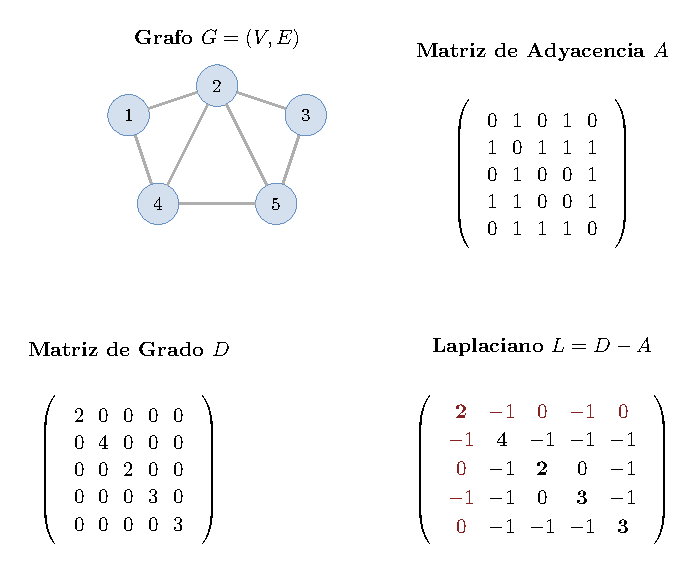
\includegraphics[width=0.8\textwidth]{images/graph_laplacian.pdf}
\caption[Matrices del Laplaciano de un grafo]{Ejemplo concreto de las matrices asociadas a un grafo: matriz de adyacencia $A$, matriz de grados $D$ y Laplaciano $L_G = D - A$. Las entradas del Laplaciano codifican la conectividad local: $L_{ii} = \deg(i)$ y $L_{ij} = -W_{ij}$ para vértices adyacentes.}
\label{fig:graph_laplacian}
\end{figure}

\begin{definition}[Matriz semidefinida positiva]\label{def:semidefinida_positiva}
	Una matriz $A \in \mathbb{R}^{n \times n}$ simétrica es \textit{semidefinida positiva} (escrito $A \succeq 0$) si
	\[
		\mathbf{x}^T A \mathbf{x} \geq 0 \quad \text{para todo } \mathbf{x} \in \mathbb{R}^n.
	\]
	Si la desigualdad es estricta para todo $\mathbf{x} \neq \mathbf{0}$, se dice que $A$ es \textit{definida positiva} ($A \succ 0$). Por el \autoref{thm:espectral_matrices_simetricas} (Apéndice~\ref{ch:teoremas_complementarios}), $A \succeq 0$ si y solo si todos sus valores propios son no negativos.
\end{definition}

\begin{proposition}[Propiedades algebraicas del Laplaciano]\label{prop:propiedades_algebraicas_laplaciano}
	El Laplaciano $L_G = D - A$ de un grafo no dirigido y ponderado satisface:
	\begin{enumerate}
		\item \textbf{Simetría}: $L_G = L_G^T$
		\item \textbf{Filas suman cero}: $L_G \mathbf{1} = \mathbf{0}$
		\item \textbf{Semidefinitud positiva}: para todo $\mathbf{x} \in \mathbb{R}^n$,
		\[
			\mathbf{x}^T L_G \mathbf{x} = \frac{1}{2}\sum_{(i,j)\in E} W_{ij}(x_i - x_j)^2 \geq 0
		\]
		\item \textbf{Operador discreto}: para funciones $f: V \to \mathbb{R}$,
		\[
			(L_G f)(i) = \sum_{j\sim i} W_{ij}(f(i)-f(j))
		\]
	\end{enumerate}
\end{proposition}

\begin{proof}
	\textbf{(1) Simetría}: Por definición, $D$ es diagonal (luego simétrica) y $A$ es simétrica por ser el grafo no dirigido, luego $L_G = D - A$ es simétrica.

	\textbf{(2) Filas suman cero}: La $i$-ésima fila de $L_G$ tiene entrada diagonal $D_{ii} = \deg(i) = \sum_j A_{ij}$ y entradas $-A_{ij}$ fuera de la diagonal. Así, $\sum_j (L_G)_{ij} = \deg(i) - \sum_j A_{ij} = 0$.

	\textbf{(3) Semidefinitud positiva}: Para cualquier $\mathbf{x} \in \mathbb{R}^n$:
	\begin{align}
		\mathbf{x}^T L_G \mathbf{x} &= \mathbf{x}^T (D - A) \mathbf{x} = \mathbf{x}^T D \mathbf{x} - \mathbf{x}^T A \mathbf{x}\\
		&= \sum_{i=1}^n D_{ii} x_i^2 - \sum_{i,j=1}^n A_{ij} x_i x_j\\
		&= \sum_{i=1}^n x_i^2 \sum_{j} A_{ij} - \sum_{i,j=1}^n A_{ij} x_i x_j\\
		&= \sum_{i,j=1}^n A_{ij} (x_i^2 - x_i x_j)\\
		&= \frac{1}{2} \sum_{i,j=1}^n A_{ij} (x_i^2 - 2x_i x_j + x_j^2)\\
		&= \frac{1}{2} \sum_{(i,j) \in E} W_{ij} (x_i - x_j)^2 \geq 0
	\end{align}

	\textbf{(4) Operador discreto}: Por definición:
	\[
		(L_G f)(i) = (Df)(i) - (Af)(i) = \sum_{j} A_{ij} f(i) - \sum_{j} A_{ij} f(j) = \sum_{j \sim i} W_{ij}(f(i) - f(j)) \qedhere
	\]
\end{proof}

\begin{proposition}[Propiedades espectrales del Laplaciano]\label{prop:propiedades_espectrales_laplaciano_grafos}
	Sea $L_G$ el Laplaciano de un grafo no dirigido con $n$ vértices. Entonces:
	\begin{enumerate}
		\item Los valores propios satisfacen $0 = \lambda_1 \leq \lambda_2 \leq \cdots \leq \lambda_n$
		\item La multiplicidad de $\lambda_1 = 0$ es igual al número de componentes conexas de $G$
	\end{enumerate}
\end{proposition}

\begin{proof}
	\textbf{(1)}: Por la \autoref{prop:propiedades_algebraicas_laplaciano}, $L_G$ es simétrico y semidefinido positivo (\autoref{def:semidefinida_positiva}). El \autoref{thm:espectral_matrices_simetricas} (Apéndice~\ref{ch:teoremas_complementarios}) garantiza que todos los valores propios son reales, y la semidefinitud positiva implica $\lambda_i \geq 0$ por el \autoref{cor:caracterizacion_semidefinida}. Además, $L_G \mathbf{1} = \mathbf{0}$ (ítem 2 de la \autoref{prop:propiedades_algebraicas_laplaciano}), por lo que $\lambda_1 = 0$ con autovector $\mathbf{1}$.

	\textbf{(2)}: $L_G \mathbf{x} = \mathbf{0}$ si y solo si $\mathbf{x}^T L_G \mathbf{x} = 0$, que por la forma cuadrática de la \autoref{prop:propiedades_algebraicas_laplaciano} equivale a $(x_i - x_j)^2 = 0$ para toda arista $(i,j) \in E$, es decir, $\mathbf{x}$ es constante en cada componente conexa. El espacio de tales vectores tiene dimensión igual al número de componentes conexas.
\end{proof}

La forma cuadrática $f^T L_G f$ mide la \textbf{suavidad} de la función $f$ sobre el grafo: es pequeña cuando $f$ varía poco entre vértices adyacentes, grande cuando hay cambios abruptos. Esta interpretación conecta con la \textbf{energía de Dirichlet} en análisis funcional \citep[Cap.~1]{Chung1997}.

\paragraph{Conexión con Geometría Diferencial}

El Laplaciano de grafo $L_G$ es el análogo discreto del operador de Laplace-Beltrami $\Delta_\mathcal{M}$ en variedades riemannianas (\autoref{def:laplace_beltrami}), que actúa sobre funciones suaves $f: \mathcal{M} \to \mathbb{R}$ como $\Delta_\mathcal{M} f = \operatorname{div}(\operatorname{grad} f)$.

La analogía es profunda:
\begin{itemize}
	\item \textbf{En variedades continuas}: $\Delta_\mathcal{M} f = \text{div}(\text{grad } f)$ mide la divergencia del gradiente
	\item \textbf{En grafos discretos}: $(L_G f)(i) = \sum_{j \sim i} (f(i) - f(j))$ mide la diferencia entre $f(i)$ y el promedio de sus vecinos
\end{itemize}

Ambos operadores generalizan el laplaciano euclidiano $\nabla^2 f$ (\autoref{def:laplaciano_euclidiano}) a dominios no euclidianos.

\subsection{Topological Deep Learning}\label{subsec:tdl_grafos}

El Laplaciano $L_G = D - A$ de la \autoref{subsec:geometria_topologica_grafos} opera exclusivamente sobre señales de nodos (0-cadenas). Sin embargo, los complejos simpliciales introducidos en la \autoref{def:complejo_simplicial} poseen una estructura algebraica mucho más rica: señales definidas sobre aristas, triángulos y símplices de orden superior. Para cuantificar esta estructura, introducimos las herramientas de la topología algebraica.

\begin{definition}[Cadenas]\label{def:cadenas_gdl}
	Sea $\mathcal{K}$ un complejo simplicial. Una \textit{$k$-cadena} es una combinación lineal formal de $k$-simplejos con coeficientes en un cuerpo (típicamente $\mathbb{R}$ o $\mathbb{Z}_2$):
	\[
		C_k(\mathcal{K}) = \left\{ \sum_{i} \alpha_i \sigma_i^{(k)} : \alpha_i \in \mathbb{R}, \, \sigma_i^{(k)} \in \mathcal{K} \text{ es un } k\text{-simplejo} \right\}
	\]
\end{definition}

\begin{definition}[Operador de frontera]\label{def:operador_frontera_gdl}
	Sea $\mathcal{K}$ un complejo simplicial. El \textit{operador de frontera} $\partial_k: C_k(\mathcal{K}) \to C_{k-1}(\mathcal{K})$ se define sobre un $k$-simplejo orientado $[v_0, v_1, \ldots, v_k]$ como:
	\[
		\partial_k [v_0, v_1, \ldots, v_k] = \sum_{i=0}^{k} (-1)^i [v_0, \ldots, \widehat{v_i}, \ldots, v_k]
	\]
	donde $\widehat{v_i}$ indica omisión del vértice $v_i$.
\end{definition}

\begin{proposition}[Propiedad fundamental del operador de frontera]\label{prop:frontera_cuadrado_cero}
	El operador de frontera satisface $\partial_{k-1} \circ \partial_k = 0$ para todo $k$. Es decir, la frontera de una frontera es vacía.
\end{proposition}

\begin{proof}
	Basta verificar la identidad sobre un $k$-simplejo orientado $[v_0, \ldots, v_k]$:
	\begin{align*}
		\partial_{k-1}(\partial_k [v_0, \ldots, v_k]) &= \partial_{k-1}\!\left(\sum_{i=0}^{k} (-1)^i [v_0, \ldots, \widehat{v_i}, \ldots, v_k]\right) \\
		&= \sum_{i=0}^{k} (-1)^i \sum_{\substack{j=0 \\ j \neq i}}^{k} (-1)^{j'} [v_0, \ldots, \widehat{v_i}, \ldots, \widehat{v_j}, \ldots, v_k]
	\end{align*}
	donde $j' = j$ si $j < i$ y $j' = j-1$ si $j > i$. Cada cara de codimensión 2, obtenida al omitir dos vértices $v_i$ y $v_j$ con $i < j$, aparece exactamente dos veces: una con signo $(-1)^{i+j}$ (omitiendo primero $v_i$ y luego $v_j$) y otra con signo $(-1)^{i+j-1}$ (omitiendo primero $v_j$ y luego $v_i$). Como $(-1)^{i+j} + (-1)^{i+j-1} = 0$, todos los términos se cancelan.
\end{proof}

\begin{definition}[Grupos de homología]\label{def:homologia_betti}
	Los \textit{grupos de homología} de un complejo simplicial $\mathcal{K}$ se definen como:
	\[
		H_k(\mathcal{K}) = \ker(\partial_k) / \mathrm{im}(\partial_{k+1}) = Z_k(\mathcal{K}) / B_k(\mathcal{K})
	\]
	donde $Z_k = \ker(\partial_k)$ son los \textit{$k$-ciclos} (cadenas sin frontera) y $B_k = \mathrm{im}(\partial_{k+1})$ son las \textit{$k$-fronteras} (cadenas que son frontera de algo).
\end{definition}

\begin{definition}[Números de Betti]\label{def:numeros_betti_gdl}
	El \textit{$k$-ésimo número de Betti} de un complejo simplicial $\mathcal{K}$ es $\beta_k = \dim H_k(\mathcal{K})$, que cuenta:
	\begin{itemize}
		\item $\beta_0$: número de componentes conexas
		\item $\beta_1$: número de ``agujeros'' o ciclos independientes
		\item $\beta_2$: número de cavidades tridimensionales
	\end{itemize}
\end{definition}

\begin{example}[Números de Betti de superficies]\label{ex:betti_superficies}
\leavevmode
	\begin{itemize}
		\item \textbf{Esfera $S^2$}: $\beta_0 = 1$ (conexa), $\beta_1 = 0$ (sin agujeros), $\beta_2 = 1$ (una cavidad)
		\item \textbf{Toro $T^2$}: $\beta_0 = 1$, $\beta_1 = 2$ (dos ciclos independientes), $\beta_2 = 1$
		\item \textbf{Botella de Klein}: $\beta_0 = 1$, $\beta_1 = 1$ (sobre $\mathbb{Z}_2$)
	\end{itemize}
\end{example}

El \textbf{\gls{TDL}} extiende el paso de mensajes (\autoref{def:mpnn_unificador}) y el análisis en grafos a estas estructuras de orden superior mediante el \textit{Laplaciano de Hodge}, que generaliza $L_G$ a $k$-cadenas arbitrarias.

\subsubsection{El Laplaciano de Hodge}\label{subsubsec:hodge_laplacian_gdl}

El operador de frontera $\partial_k$ (\autoref{def:operador_frontera_gdl}) y la propiedad $\partial_{k-1} \circ \partial_k = 0$ (\autoref{prop:frontera_cuadrado_cero}) proporcionan la secuencia de espacios de cadenas:
\[
	\cdots \xrightarrow{\partial_{k+2}} C_{k+1}(\mathcal{K}) \xrightarrow{\partial_{k+1}} C_k(\mathcal{K}) \xrightarrow{\partial_k} C_{k-1}(\mathcal{K}) \xrightarrow{\partial_{k-1}} \cdots
\]

\begin{definition}[Operador cofrontera]\label{def:operador_cofrontera_gdl}
	Equipamos cada espacio de cadenas $C_k(\mathcal{K})$ con el \textit{producto interior estándar} en el que los $k$-símplices orientados forman una base ortonormal. El \textit{operador cofrontera} $\partial_k^T : C_{k-1}(\mathcal{K}) \to C_k(\mathcal{K})$ es el adjunto formal del operador de frontera (\autoref{def:operador_frontera_gdl}) respecto a este producto interior, es decir, el único operador lineal que satisface:
	\[
		\langle \partial_k^T c, \, \sigma \rangle = \langle c, \, \partial_k \sigma \rangle \quad \text{para todo } c \in C_{k-1}(\mathcal{K}),\; \sigma \in C_k(\mathcal{K}).
	\]

	\textbf{Interpretación combinatoria.} Para un $(k{-}1)$-símplice $\tau$, el operador cofrontera agrega todos los $k$-símplices de $\mathcal{K}$ que contienen a $\tau$ como cara, con los signos de incidencia heredados:
	\[
		\partial_k^T(\tau) = \sum_{\substack{\sigma \in \mathcal{K} \\ \dim \sigma = k}} [\partial_k]_{\tau\sigma} \, \sigma,
	\]
	donde $[\partial_k]_{\tau\sigma}$ denota el coeficiente de $\tau$ en $\partial_k(\sigma)$, que es $(-1)^i$ si $\tau$ se obtiene de $\sigma$ omitiendo su $i$-ésimo vértice, y $0$ si $\tau$ no es cara de $\sigma$.

	\textbf{Complejo de cocadenas.} Los operadores cofrontera revierten la dirección del complejo de cadenas, formando el \textit{complejo de cocadenas}:
	\[
		\cdots \xleftarrow{\partial_{k+2}^T} C_{k+1}(\mathcal{K}) \xleftarrow{\partial_{k+1}^T} C_k(\mathcal{K}) \xleftarrow{\partial_k^T} C_{k-1}(\mathcal{K}) \xleftarrow{\partial_{k-1}^T} \cdots
	\]

	\textbf{Nilpotencia.} Transponiendo $\partial_{k} \circ \partial_{k+1} = 0$ (\autoref{prop:frontera_cuadrado_cero}) se obtiene $\partial_{k+1}^T \circ \partial_k^T = 0$, lo que garantiza que la secuencia anterior es efectivamente un complejo de cocadenas.
\end{definition}

\begin{definition}[Laplaciano de Hodge]\label{def:hodge_laplacian_gdl}
	Sea $\mathcal{K}$ un complejo simplicial finito con operadores de frontera $\partial_k$. El \textit{Laplaciano de Hodge de orden $k$} es el operador $L_k: C_k(\mathcal{K}) \to C_k(\mathcal{K})$ definido por:
	\[
		L_k = \underbrace{\partial_k^T \partial_k}_{L_k^{\mathrm{down}}} + \underbrace{\partial_{k+1} \partial_{k+1}^T}_{L_k^{\mathrm{up}}}
	\]
	donde:
	\begin{itemize}
		\item $L_k^{\mathrm{down}} = \partial_k^T \partial_k$ captura adyacencia \textit{inferior}: dos $k$-símplices son adyacentes si comparten una $(k{-}1)$-cara.
		\item $L_k^{\mathrm{up}} = \partial_{k+1} \partial_{k+1}^T$ captura adyacencia \textit{superior}: dos $k$-símplices son adyacentes si pertenecen a un mismo $(k{+}1)$-símplice.
	\end{itemize}
\end{definition}

\begin{proposition}[Propiedades del Laplaciano de Hodge]\label{prop:propiedades_hodge_gdl}
	El Laplaciano de Hodge $L_k$ satisface:
	\begin{enumerate}
		\item \textbf{Simetría y semidefinición positiva}: $L_k$ es simétrica y $\langle x, L_k x \rangle \geq 0$ para toda $k$-cadena $x$, pues $L_k$ es suma de matrices de Gram: $\langle x, \partial_k^T \partial_k x \rangle = \|\partial_k x\|^2 \geq 0$ y $\langle x, \partial_{k+1} \partial_{k+1}^T x \rangle = \|\partial_{k+1}^T x\|^2 \geq 0$.
		\item \textbf{Recuperación del Laplaciano de grafos}: Para $k = 0$, como $\partial_0 = 0$ por convención, se tiene $L_0 = \partial_1 \partial_1^T$, que coincide con el Laplaciano $L_G = D - A$ de la \autoref{def:laplaciano_grafo}.
		\item \textbf{Conexión con homología}: $\ker(L_k) \cong H_k(\mathcal{K})$, es decir, las $k$-cadenas armónicas corresponden al $k$-ésimo grupo de homología. Este resultado es corolario inmediato del \autoref{thm:hodge_decomposition_gdl}.
	\end{enumerate}
\end{proposition}

\begin{proof}
	\textbf{(1)}: $L_k$ es simétrica por ser suma de matrices de Gram: $(\partial_k^T \partial_k)^T = \partial_k^T \partial_k$ y $(\partial_{k+1} \partial_{k+1}^T)^T = \partial_{k+1} \partial_{k+1}^T$. Para la semidefinición positiva, sea $x \in C_k(\mathcal{K})$:
	\[
		\langle x, L_k x \rangle = \langle x, \partial_k^T \partial_k x \rangle + \langle x, \partial_{k+1} \partial_{k+1}^T x \rangle = \|\partial_k x\|^2 + \|\partial_{k+1}^T x\|^2 \geq 0.
	\]

	\textbf{(2)}: Para $k = 0$, el espacio $C_{-1}(\mathcal{K})$ es trivial, luego $\partial_0 = 0$ y $L_0 = \partial_1 \partial_1^T$. Si $\partial_1$ es la matriz de incidencia orientada del grafo, con entradas $(\partial_1)_{e,v} = +1$ si $v$ es el origen de $e$ y $-1$ si es el destino, entonces la entrada $(i,j)$ de $\partial_1 \partial_1^T$ es: $d_i$ si $i = j$ (grado del vértice), $-1$ si $(i,j) \in E$, y $0$ en caso contrario. Es decir, $\partial_1 \partial_1^T = D - A = L_G$.

	\textbf{(3)}: Por (1), $L_k x = 0$ si y solo si $\langle x, L_k x \rangle = \|\partial_k x\|^2 + \|\partial_{k+1}^T x\|^2 = 0$, lo que equivale a $\partial_k x = 0$ y $\partial_{k+1}^T x = 0$ simultáneamente. La primera condición dice $x \in Z_k = \ker(\partial_k)$; la segunda dice $x \in \mathrm{im}(\partial_{k+1})^\perp$, pues $\langle \partial_{k+1} a, x \rangle = \langle a, \partial_{k+1}^T x \rangle = 0$ para todo $a$. Así, $x$ es un ciclo ortogonal a todas las fronteras, y la clase $[x] \in Z_k / B_k = H_k(\mathcal{K})$ establece el isomorfismo $\ker(L_k) \cong H_k(\mathcal{K})$.
\end{proof}

El resultado central de la teoría de Hodge discreta proporciona una descomposición ortogonal del espacio de cadenas que generaliza el análisis de Fourier en grafos (véase la \autoref{subsec:analisis_espectral_grafos_gdl}). Para un tratamiento exhaustivo del Laplaciano de Hodge en grafos, véase \citet{lim2020hodge}.

\begin{theorem}[Descomposición de Hodge]\label{thm:hodge_decomposition_gdl}
	Para un complejo simplicial finito $\mathcal{K}$, el espacio de $k$-cadenas admite la descomposición ortogonal:
	\[
		C_k(\mathcal{K}) = \underbrace{\mathrm{im}(\partial_{k+1})}_{\text{fronteras (``gradientes'')}} \oplus \underbrace{\ker(L_k)}_{\text{armónicos}} \oplus \underbrace{\mathrm{im}(\partial_k^T)}_{\text{cofronteras (``rotacionales'')}}
	\]
	Las tres componentes capturan aspectos complementarios de una señal simplicial: las fronteras representan flujo irrotacional, los armónicos codifican la topología global ($H_k$), y las cofronteras representan circulación pura.
\end{theorem}

\begin{proof}
	Debemos demostrar que los tres subespacios $\mathrm{im}(\partial_{k+1})$, $\ker(L_k)$ y $\mathrm{im}(\partial_k^T)$ son mutuamente ortogonales y que su suma directa es $C_k(\mathcal{K})$.

	\textbf{Paso 1: Ortogonalidad mutua.} Sean $x \in \mathrm{im}(\partial_{k+1})$ e $y \in \mathrm{im}(\partial_k^T)$. Entonces $x = \partial_{k+1} a$ para algún $a \in C_{k+1}$ e $y = \partial_k^T b$ para algún $b \in C_{k-1}$. Usando la propiedad $\partial_k \circ \partial_{k+1} = 0$ (\autoref{prop:frontera_cuadrado_cero}):
	\[
		\langle x, y \rangle = \langle \partial_{k+1} a, \partial_k^T b \rangle = \langle \partial_k \partial_{k+1} a, b \rangle = \langle 0, b \rangle = 0.
	\]
	Ahora, sea $z \in \ker(L_k)$. De la demostración de la \autoref{prop:propiedades_hodge_gdl}(3), $L_k z = 0$ implica $\partial_k z = 0$ y $\partial_{k+1}^T z = 0$. Entonces:
	\[
		\langle z, \partial_{k+1} a \rangle = \langle \partial_{k+1}^T z, a \rangle = 0, \qquad
		\langle z, \partial_k^T b \rangle = \langle \partial_k z, b \rangle = 0.
	\]
	Los tres subespacios son, por tanto, mutuamente ortogonales.

	\textbf{Paso 2: Completitud.} Para complejos simpliciales finitos, todos los espacios son de dimensión finita, por lo que basta verificar que $C_k = V_1 \oplus V_2 \oplus V_3$ donde $V_1 = \mathrm{im}(\partial_{k+1})$, $V_2 = \mathrm{im}(\partial_k^T)$ y $V_3 = \ker(L_k)$. Sea $w \in (V_1 \oplus V_2)^\perp$. Entonces $w \perp \mathrm{im}(\partial_{k+1})$ y $w \perp \mathrm{im}(\partial_k^T)$, lo que implica:
	\[
		\partial_{k+1}^T w = 0 \quad \text{y} \quad \partial_k w = 0.
	\]
	Por tanto $L_k w = \partial_k^T \partial_k w + \partial_{k+1} \partial_{k+1}^T w = 0$, es decir, $w \in \ker(L_k)$. Esto demuestra $(V_1 \oplus V_2)^\perp = V_3$, y así $C_k = V_1 \oplus V_2 \oplus V_3$.
\end{proof}

La descomposición de Hodge tiene una importancia central para el \gls{GDL} por las siguientes razones:
\begin{itemize}
	\item \textbf{Generalización del análisis de Fourier}: mientras que la diagonalización de $L_0$ proporciona la transformada de Fourier en grafos (véase la \autoref{subsec:analisis_espectral_grafos_gdl}), la descomposición de Hodge extiende este análisis a señales sobre símplices de cualquier orden $k$.
	\item \textbf{Interpretación física de las componentes}: toda señal simplicial se descompone en un componente gradiente $\mathrm{im}(\partial_{k+1})$ (flujo irrotacional), un componente armónico $\ker(L_k)$ (topología global) y un componente rotacional $\mathrm{im}(\partial_k^T)$ (circulación pura), análogamente a la descomposición de Helmholtz en campos vectoriales.
	\item \textbf{Detección de características topológicas}: la componente armónica satisface $\ker(L_k) \cong H_k(\mathcal{K})$, lo que permite a las redes neuronales simpliciales acceder directamente a la información homológica del complejo.
\end{itemize}
Las extensiones de esta descomposición a mecanismos de atención simplicial se desarrollan en el \autoref{ch:attention}.

\begin{example}[Laplaciano de Hodge $L_1$ de un complejo triangular]\label{ex:hodge_laplacian_triangular}
	Consideremos un complejo simplicial $\mathcal{K}$ con vértices $\{a, b, c, d\}$, aristas $e_1 = [a,b]$, $e_2 = [b,c]$, $e_3 = [a,c]$, $e_4 = [c,d]$, y un único 2-símplice $\sigma = [a,b,c]$. La matriz del operador de frontera $\partial_2: C_2 \to C_1$ se obtiene de $\partial_2[a,b,c] = [b,c] - [a,c] + [a,b] = e_2 - e_3 + e_1$:
	\[
		\partial_2 = \begin{pmatrix} 1 \\ 1 \\ -1 \\ 0 \end{pmatrix} \quad \text{(columna correspondiente a $\sigma$)}
	\]
	y la matriz $\partial_1: C_1 \to C_0$ es:
	\[
		\partial_1 = \begin{pmatrix} -1 & 0 & -1 & 0 \\ 1 & -1 & 0 & 0 \\ 0 & 1 & 1 & -1 \\ 0 & 0 & 0 & 1 \end{pmatrix}
	\]
	Puede verificarse que $\partial_1 \partial_2 = 0$, como exige la \autoref{prop:frontera_cuadrado_cero}. Entonces:
	\[
		L_1^{\mathrm{down}} = \partial_1^T \partial_1 = \begin{pmatrix} 2 & -1 & 1 & 0 \\ -1 & 2 & 1 & -1 \\ 1 & 1 & 2 & -1 \\ 0 & -1 & -1 & 2 \end{pmatrix}, \quad
		L_1^{\mathrm{up}} = \partial_2 \partial_2^T = \begin{pmatrix} 1 & 1 & -1 & 0 \\ 1 & 1 & -1 & 0 \\ -1 & -1 & 1 & 0 \\ 0 & 0 & 0 & 0 \end{pmatrix}
	\]
	Nótese cómo $L_1^{\mathrm{down}}$ conecta aristas que comparten un vértice (adyacencia inferior), mientras que $L_1^{\mathrm{up}}$ conecta aristas que coexisten en el triángulo $\sigma$ (adyacencia superior). La arista $e_4$, que no pertenece a ningún triángulo, tiene $L_1^{\mathrm{up}}$ nula en su fila/columna.
\end{example}

\subsubsection{Paso de Mensajes en Complejos Simpliciales}\label{subsubsec:message_passing_simplicial_gdl}

La descomposición $L_k = L_k^{\mathrm{down}} + L_k^{\mathrm{up}}$ revela que cada $k$-símplice recibe información de dos fuentes geométricamente distintas: sus $(k{-}1)$-caras (adyacencia inferior) y los $(k{+}1)$-símplices que lo contienen (adyacencia superior). Esta estructura dual motiva una generalización natural del paso de mensajes en grafos a complejos simpliciales, cuya formalización como instancia del marco \gls{MPNN} se desarrolla en la \autoref{subsubsec:tdl_mpnn_general}.

\subsubsection{Variantes Arquitectónicas y Extensiones}\label{subsubsec:variantes_tdl}

El marco de \gls{TDL} presentado en esta sección admite diversas especializaciones y extensiones, tratadas en detalle en los capítulos siguientes:

\begin{itemize}
	\item \textbf{Convoluciones topológicas}: Filtros espectrales sobre el Laplaciano de Hodge, parametrizados mediante polinomios de $L_k$. Véase la \autoref{def:hodge_laplacians_cnn} del \autoref{ch:cnn}.
	\item \textbf{Atención simplicial}: Mecanismos de atención que ponderan los mensajes simplicial según la orientación y relevancia topológica. Véase la \autoref{def:mensaje_simplicial} del \autoref{ch:attention} y \citep{giusti2022simplicial}.
	\item \textbf{Complejos celulares}: Generalización de complejos simpliciales donde las células de dimensión $k$ pueden tener forma arbitraria (no solo símplices). Véase la \autoref{def:complejo_celular} del \autoref{ch:cnn} y \citep{bodnar2021cellular}.
	\item \textbf{Difusión simplicial}: Extensión de la ecuación de difusión a complejos simpliciales mediante $L_k$. Véase la \autoref{def:ecuacion_difusion_simplicial} del \autoref{ch:attention}.
	\item \textbf{Redes de atención de orden superior}: Arquitecturas que combinan atención multi-cabeza con topología simplicial \citep{hajij2022higherorder, hajij2023topological}.
\end{itemize}

\subsection{Convergencia de Grafos a Variedades}\label{subsec:convergencia_grafos_variedades}

La pregunta fundamental que conecta la teoría de grafos con la geometría diferencial es: \textbf{¿bajo qué condiciones un grafo discreto aproxima fielmente una variedad continua?} El siguiente teorema, uno de los resultados centrales en la teoría de aprendizaje de variedades, conecta conceptos de análisis en variedades, teoría de grafos aleatorios y análisis asintótico para proporcionar una respuesta rigurosa.

\begin{theorem}[Convergencia de grafos a variedades]\label{thm:convergencia_grafos_variedades_detallado}
	Sea $(\mathcal{M}, g)$ una variedad riemanniana compacta de dimensión $d$ inmersa en $\mathbb{R}^N$. Sea $\{x_1, \ldots, x_n\}$ una muestra de puntos en $\mathcal{M}$ distribuidos según una densidad $p(x)$ acotada por abajo: $p(x) \geq p_{\min} > 0$. Construimos un grafo $G_n$ con matriz de pesos $W_{ij} = k_\epsilon(\|x_i - x_j\|)$ donde $k_\epsilon(t) = \frac{1}{\epsilon^d} k\left(\frac{t}{\epsilon}\right)$ y $k: \mathbb{R}_+ \to \mathbb{R}_+$ es un kernel radial suave con soporte compacto.

	Entonces, bajo las condiciones de escalamiento:
	\begin{itemize}
		\item $\epsilon = \epsilon_n \to 0$ cuando $n \to \infty$
		\item $n\epsilon^{d+2} \to \infty$ (suficientes vecinos por nodo)
	\end{itemize}

	el Laplaciano normalizado del grafo converge al operador de Laplace-Beltrami ponderado:
	\[
		\lim_{n \to \infty} \frac{1}{p(x_i)\,\epsilon^2} L_n f(x_i) = \Delta_\mathcal{M} f(x_i) + \langle \nabla \log p(x_i), \nabla f(x_i) \rangle
	\]
	donde $L_n$ es el operador de Laplaciano del grafo definido en el Paso~1 de la demostración y la convergencia es en probabilidad uniformemente para $f \in C^2(\mathcal{M})$.
\end{theorem}

\begin{proof}
	La demostración procede en siete pasos, combinando técnicas de geometría diferencial, análisis funcional y teoría de probabilidad.

	\textbf{Paso 1: Normalización del Laplaciano del grafo.}

	Definimos el Laplaciano normalizado por densidad como:
	\[
		L_n f(x_i) = \frac{1}{n \epsilon^d} \sum_{j=1}^n k_\epsilon(\|x_i - x_j\|) [f(x_j) - f(x_i)]
	\]
	donde $k_\epsilon(t) = \frac{1}{\epsilon^d} k\left(\frac{t}{\epsilon}\right)$ normaliza apropiadamente el kernel. El factor $n\epsilon^d$ representa el volumen local esperado del vecindario.

	\textbf{Paso 2: Aproximación local mediante coordenadas normales.}

	Para $x_i \in \mathcal{M}$, trabajamos en coordenadas geodésicas normales centradas en $x_i$. En estas coordenadas, la métrica riemanniana satisface:
	\[
		g_{jk}(y) = \delta_{jk} + O(\|y\|^2)
	\]
	es decir, la variedad se aproxima localmente por su espacio tangente $T_{x_i}\mathcal{M} \cong \mathbb{R}^d$.

	Para puntos $x_j$ cercanos a $x_i$ con $\|x_i - x_j\| < \epsilon$, podemos escribir:
	\[
		x_j = \exp_{x_i}(\epsilon v_j)
	\]
	donde $v_j \in T_{x_i}\mathcal{M}$ con $\|v_j\| \leq C$ para alguna constante $C$, y $\exp$ denota el mapa exponencial.

	\textbf{Paso 3: Expansión de Taylor de $f$.}

	Usando la expansión de Taylor de $f$ alrededor de $x_i$ en la variedad:
	\begin{align}
		f(x_j) - f(x_i) &= f(\exp_{x_i}(\epsilon v_j)) - f(x_i)\\
		&= \epsilon \langle \nabla f(x_i), v_j \rangle + \frac{\epsilon^2}{2} \text{Hess}_f(x_i)(v_j, v_j) + O(\epsilon^3)
	\end{align}
	donde:
	\begin{itemize}
		\item $\nabla f(x_i) \in T_{x_i}\mathcal{M}$ es el gradiente riemanniano de $f$
		\item $\text{Hess}_f(x_i): T_{x_i}\mathcal{M} \times T_{x_i}\mathcal{M} \to \mathbb{R}$ es el Hessiano intrínseco de $f$
	\end{itemize}

	\textbf{Paso 4: Cálculo del límite esperado.}

	Sustituyendo la expansión en $L_n f(x_i)$:
	\begin{align}
		\frac{1}{\epsilon^2} L_n f(x_i) &= \frac{1}{n \epsilon^{d+2}} \sum_{j=1}^n k_\epsilon(\|x_i - x_j\|) [f(x_j) - f(x_i)]\\
		&= \frac{1}{n \epsilon^{d+2}} \sum_{j=1}^n k_\epsilon(\|x_i - x_j\|) \left[\epsilon \langle \nabla f(x_i), v_j \rangle + \frac{\epsilon^2}{2} \text{Hess}_f(x_i)(v_j,v_j)\right]\\
		&\quad + O(\epsilon)
	\end{align}

	\textbf{Paso 5: Promedio asintótico y ley de grandes números.}

	Cuando $n \to \infty$, por la ley fuerte de los grandes números (los puntos $\{x_j\}$ son i.i.d. con densidad $p$):
	\[
		\frac{1}{n} \sum_{j=1}^n F(x_j) \xrightarrow{\text{a.s.}} \mathbb{E}[F] = \int_{\mathcal{M}} F(y) \, p(y) \, dV_g(y)
	\]

	Aplicando esto al término de primer orden:
	\begin{align}
		&\frac{1}{n\epsilon^{d+1}} \sum_{j=1}^n k_\epsilon(\|x_i - x_j\|) \langle \nabla f(x_i), v_j \rangle\\
		&\approx \frac{1}{\epsilon^{d+1}} \int_{\mathcal{M}} k_\epsilon(\|x_i - y\|) \langle \nabla f(x_i), v(y) \rangle \, p(y) \, dV_g(y)
	\end{align}

	Cambiando variables a $y = \exp_{x_i}(\epsilon v)$ y expandiendo la densidad $p(\exp_{x_i}(\epsilon v)) = p(x_i) + \epsilon \langle \nabla p(x_i), v \rangle + O(\epsilon^2)$:
	\[
		\approx \int_{T_{x_i}\mathcal{M}} k(\|v\|) \langle \nabla f(x_i), v \rangle \, \bigl[p(x_i) + \epsilon \langle \nabla p(x_i), v \rangle\bigr] \, dv
	\]

	\textbf{Paso 6: Análisis del término de primer orden.}

	El término $p(x_i) \int k(\|v\|) \langle \nabla f, v \rangle \, dv = 0$ se anula por simetría radial de $k$. Sin embargo, el término cruzado de orden $\epsilon$:
	\[
		\epsilon \int_{T_{x_i}\mathcal{M}} k(\|v\|) \langle \nabla f(x_i), v \rangle \langle \nabla p(x_i), v \rangle \, dv
	\]
	no se anula en general, pues el integrando contiene productos $v_\alpha v_\beta$ que sobreviven a la integración cuando $\alpha = \beta$. Por simetría radial, $\int k(\|v\|) v_\alpha v_\beta \, dv = \frac{1}{d}\left(\int k(\|v\|) \|v\|^2 \, dv\right) \delta_{\alpha\beta}$, de modo que este término contribuye proporcionalmente a $\langle \nabla f(x_i), \nabla p(x_i) \rangle$.

	\textbf{Paso 7: Término principal de segundo orden y resultado final.}

	El término de segundo orden da:
	\begin{align}
		\frac{p(x_i)}{2} \int_{T_{x_i}\mathcal{M}} k(\|v\|) \text{Hess}_f(x_i)(v,v) \, dv
	\end{align}

	Usando la relación $\text{tr}(\text{Hess}_f) = \Delta_\mathcal{M} f$ (traza del Hessiano es el Laplaciano) y la simetría radial:
	\begin{align}
		&= \frac{p(x_i)}{2d} \left(\int_{\mathbb{R}^d} k(\|v\|) \|v\|^2 \, dv\right) \Delta_\mathcal{M} f(x_i)
	\end{align}

	Eligiendo el kernel $k$ tal que $\int_{\mathbb{R}^d} k(\|v\|) \|v\|^2 \, dv = 2d$, combinando los términos de los Pasos~6 y~7:
	\[
		\lim_{n \to \infty} \frac{1}{\epsilon^2} L_n f(x_i) = p(x_i) \Delta_\mathcal{M} f(x_i) + \langle \nabla p(x_i), \nabla f(x_i) \rangle
	\]

	Dividiendo por $p(x_i)$ y usando que $\nabla p / p = \nabla \log p$:
	\[
		\lim_{n \to \infty} \frac{1}{p(x_i)\,\epsilon^2} L_n f(x_i) = \Delta_\mathcal{M} f(x_i) + \langle \nabla \log p(x_i), \nabla f(x_i) \rangle
	\]

	El término $\langle \nabla \log p, \nabla f \rangle$ refleja la influencia de la densidad de muestreo no uniforme y puede eliminarse con construcciones más sofisticadas del Laplaciano \citep{coifman2006diffusion, hein2007graph}.

	\textbf{Condiciones técnicas:} La convergencia requiere que $\epsilon \to 0$ (radio local tiende a cero) pero $n\epsilon^{d+2} \to \infty$ (suficientes puntos en cada vecindario). La tasa óptima es:
	\[
		\epsilon \sim \left(\frac{\log n}{n}\right)^{1/(d+2+\alpha)}
	\]
	para algún $\alpha > 0$ pequeño, balanceando el sesgo de la aproximación con la varianza del muestreo.
\end{proof}

\paragraph{Implicaciones para Geometric Deep Learning}

Este resultado teórico fundamental tiene consecuencias profundas para el \gls{GDL}:

\begin{enumerate}
	\item \textbf{Justificación teórica de GNNs}: Los grafos pueden capturar fielmente la geometría de variedades cuando tenemos suficientes datos. Esto justifica el uso de \glspl{GNN} para datos que residen naturalmente en variedades.

	\item \textbf{Guía para construcción de grafos}: Las condiciones del teorema ($\epsilon \to 0$, $n\epsilon^{d+2} \to \infty$) proporcionan principios para elegir el radio de vecindad $\epsilon$ en función del número de muestras $n$ y la dimensión intrínseca $d$.

	\item \textbf{Limitaciones fundamentales}: Los datos son finitos, por lo que solo tenemos aproximaciones. La construcción del grafo (elección de $\epsilon$, tipo de kernel) afecta la calidad de la aproximación. Se pierde información sobre la geometría suave entre puntos muestreados.

	\item \textbf{Trade-off computacional}: Trabajar directamente con variedades continuas es matemáticamente elegante pero computacionalmente intratable. Los grafos ofrecen un compromiso práctico entre expresividad geométrica y eficiencia computacional.

	\item \textbf{Diseño de arquitecturas}: Las \glspl{GNN} que aproximan filtros espectrales del Laplaciano heredan propiedades geométricas del dominio continuo, motivando arquitecturas como ChebNet y GCN.
\end{enumerate}

La perspectiva unificadora es clara: \textbf{los grafos son paso intermedio entre representaciones euclidianas (que ignoran geometría) y variedades continuas (que son matemáticamente elegantes pero computacionalmente costosas)}. Tanto grafos como variedades preservan mejor la estructura intrínseca de los datos que las representaciones vectoriales tradicionales, pero con diferentes compromisos entre precisión geométrica y factibilidad computacional.

\begin{remark}[Tasas de convergencia y regímenes de escalamiento]\label{rem:tasas_convergencia_laplaciano}
	La convergencia del Laplaciano del grafo al operador de Laplace-Beltrami depende críticamente de la relación entre $n$ (número de puntos) y $\epsilon$ (radio de conectividad). Se identifican tres regímenes:

	\begin{center}
	\small
	\begin{tabular}{@{}llp{5cm}@{}}
		\toprule
		\textbf{Régimen} & \textbf{Condición} & \textbf{Comportamiento} \\
		\midrule
		Subconectado & $n\epsilon^d \to 0$ & Grafo desconectado; no hay convergencia \\
		\addlinespace
		Óptimo & $n\epsilon^d \sim \log n$ & Convergencia con tasa $O(\epsilon^2 + 1/\sqrt{n\epsilon^d})$ \\
		\addlinespace
		Sobreconectado & $n\epsilon^d \to \infty$ muy rápido & Convergencia, pero pérdida de localidad \\
		\bottomrule
	\end{tabular}
	\end{center}

	\textbf{Ejemplo numérico (esfera $S^2$, $d=2$):} Para $n = 10000$ puntos uniformemente distribuidos en $S^2$:
	\begin{itemize}
		\item $\epsilon = 0.05$: Error en primer autovalor no trivial $\approx 15\%$ (subconectado)
		\item $\epsilon = 0.15$: Error $\approx 2\%$ (régimen óptimo)
		\item $\epsilon = 0.40$: Error $\approx 5\%$ (sobreconectado, pierde localidad)
	\end{itemize}
	La elección óptima $\epsilon^* \approx (\log n / n)^{1/4} \approx 0.14$ coincide con las predicciones teóricas.
\end{remark}

\subsection{Análisis Espectral en Grafos}\label{subsec:analisis_espectral_grafos_gdl}

El \textbf{análisis espectral de grafos} extiende las ideas del análisis de Fourier clásico al dominio discreto (los fundamentos del análisis armónico y la transformada de Fourier se desarrollan en la \autoref{sec:analisis_armonico} del \autoref{ch:cnn}). Los autovectores del Laplaciano forman una base ortogonal análoga a las ondas sinusoidales en el análisis de Fourier euclidiano, permitiendo descomponer funciones en "frecuencias" sobre el grafo.

\paragraph{Transformada de Fourier en Grafos}

\begin{definition}[Transformada de Fourier en grafos]\label{def:transformada_fourier_grafos}
	Sea $G = (V,E)$ un grafo con Laplaciano normalizado $\mathcal{L}$ y descomposición espectral $\mathcal{L} = U \Lambda U^T$ donde:
	\begin{itemize}
		\item $\Lambda = \text{diag}(\lambda_1, \ldots, \lambda_n)$ con $0 = \lambda_1 \leq \lambda_2 \leq \cdots \leq \lambda_n \leq 2$
		\item $U = [u_1, \ldots, u_n]$ con $u_i \in \mathbb{R}^n$ autovectores ortonormales
	\end{itemize}

	La \textit{transformada de Fourier en grafos} de una función $f: V \to \mathbb{R}$ (vista como $f \in \mathbb{R}^n$) es:
	\[
		\hat{f} = U^T f \in \mathbb{R}^n
	\]

	La \textit{transformada inversa} es:
	\[
		f = U \hat{f} = \sum_{i=1}^n \hat{f}(i) \, u_i
	\]
\end{definition}

Esta transformación descompone $f$ en las ``bases armónicas'' $\{u_i\}$ del grafo, donde $\hat{f}(i)$ representa el ``coeficiente de frecuencia'' asociado al autovalor $\lambda_i$. Nótese la analogía directa con la \autoref{def:transformada_fourier_continua}: los autovectores $u_i$ del Laplaciano juegan el papel de las exponenciales complejas $e^{2\pi i \omega \cdot x}$, y los autovalores $\lambda_i$ el de las frecuencias $\omega$.

\begin{figure}[htbp]
\centering
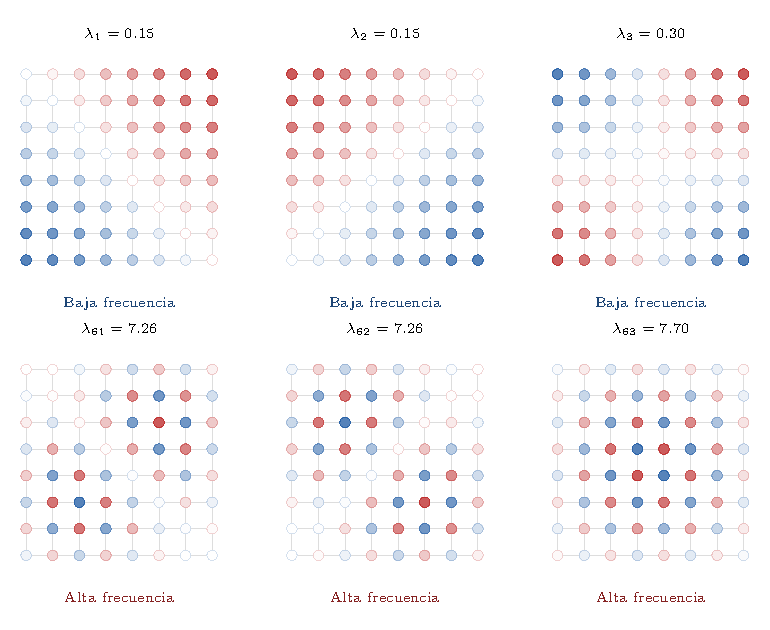
\includegraphics[width=0.95\textwidth]{images/laplacian_eigenvectors}
\caption[Autovectores del Laplaciano en grafos]{Autovectores del Laplaciano en un grafo de grilla. Los autovalores pequeños corresponden a funciones suaves (baja frecuencia), mientras que los autovalores grandes corresponden a funciones oscilatorias (alta frecuencia).}
\label{fig:laplacian_eigenvectors}
\end{figure}

\begin{theorem}[Interpretación frecuencial de autovectores]\label{thm:interpretacion_frecuencial_autovectores}
	Los autovectores del Laplaciano $\{u_i\}$ satisfacen:
	\begin{enumerate}
		\item \textbf{Autovalores pequeños $\Leftrightarrow$ funciones suaves}: Si $\mathcal{L} u_i = \lambda_i u_i$ con $\lambda_i$ pequeño, entonces:
		\[
			u_i^T \mathcal{L} u_i = \lambda_i \|u_i\|^2 = \lambda_i
		\]
		es pequeño, lo cual por la \autoref{prop:propiedades_algebraicas_laplaciano} implica que $u_i$ varía suavemente sobre el grafo.

		\item \textbf{Autovalores grandes $\Leftrightarrow$ funciones oscilatorias}: Si $\lambda_i \approx 2$, entonces $u_i$ oscila rápidamente entre valores positivos y negativos en nodos adyacentes.

		\item \textbf{Analogía con frecuencias}: $\lambda_i$ juega el rol de "frecuencia al cuadrado": $\lambda_i \sim \omega_i^2$ en el análisis de Fourier clásico (\autoref{sec:analisis_armonico}).
	\end{enumerate}
\end{theorem}

\begin{proof}
	\textbf{(1)}: Análogamente a la forma cuadrática del Laplaciano no normalizado (\autoref{prop:propiedades_algebraicas_laplaciano}), para el Laplaciano normalizado $\mathcal{L} = D^{-1/2} L_G D^{-1/2}$ se tiene:
	\[
		u_i^T \mathcal{L} u_i = \frac{1}{2} \sum_{(j,k) \in E} W_{jk} \left(\frac{u_i(j)}{\sqrt{d_j}} - \frac{u_i(k)}{\sqrt{d_k}}\right)^2
	\]

	Si $\lambda_i$ es pequeño, esta suma debe ser pequeña, lo cual requiere que $|u_i(j) - u_i(k)|$ sea pequeño para aristas $(j,k)$, es decir, $u_i$ es suave.

	\textbf{(2)}: Para el Laplaciano normalizado, $\lambda_{\max} \leq 2$. Valores cercanos a 2 se alcanzan cuando $u_i$ cambia de signo frecuentemente entre vecinos, maximizando $(u_i(j) - u_i(k))^2$.

	\textbf{(3)}: En el Laplaciano euclidiano $\nabla^2$, las eigenfunciones son ondas planas $e^{i\omega \cdot x}$ con eigenvalores $-\omega^2$. Cambiando signo (convención), $\lambda \sim \omega^2$.
\end{proof}

\begin{figure}[htbp]
\centering
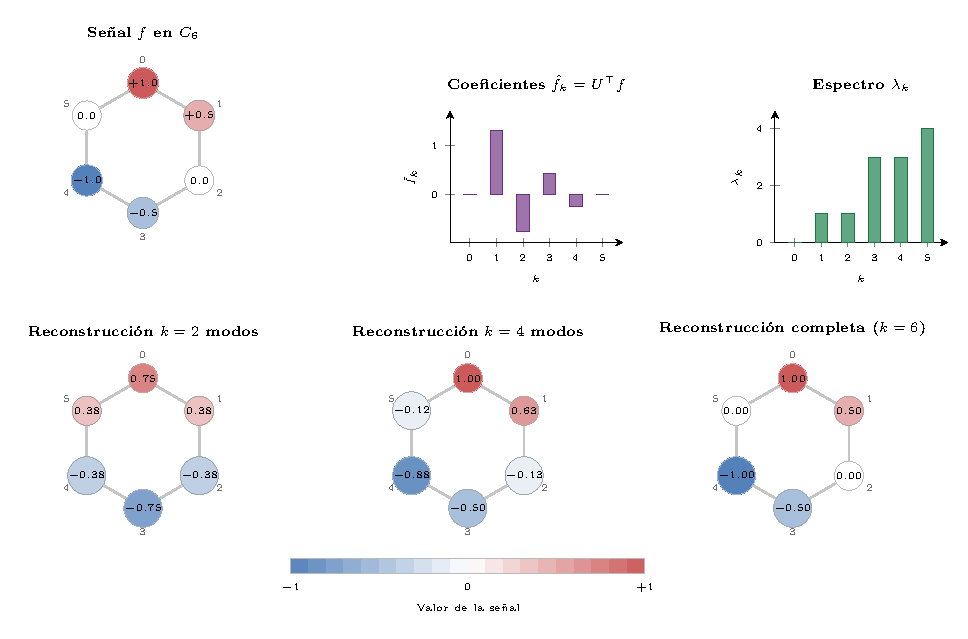
\includegraphics[width=0.95\textwidth]{images/graph_fourier_transform}
\caption[Transformada de Fourier en grafos]{Transformada de Fourier en grafos. Arriba: una señal sobre un grafo cíclico, sus coeficientes de Fourier y el espectro de frecuencias. Abajo: reconstrucción parcial usando diferentes números de modos, mostrando cómo los componentes de baja frecuencia capturan variaciones suaves.}
\label{fig:graph_fourier_transform}
\end{figure}

\paragraph{Filtros Espectrales}

La transformada de Fourier en grafos permite definir \textbf{filtros espectrales}, fundamentales para las \glspl{GNN} espectrales:

\begin{definition}[Filtro espectral en grafos]\label{def:filtro_espectral_grafo}
	Un \textit{filtro espectral} es un operador lineal $g_\theta: \mathbb{R}^n \to \mathbb{R}^n$ definido mediante una función de transferencia $g_\theta: \mathbb{R} \to \mathbb{R}$ aplicada a los autovalores del Laplaciano:
	\[
		g_\theta(\mathcal{L}) = U \, g_\theta(\Lambda) \, U^T = U \, \text{diag}(g_\theta(\lambda_1), \ldots, g_\theta(\lambda_n)) \, U^T
	\]

	La \textit{convolución espectral} de una señal $f$ con el filtro $g_\theta$ es:
	\[
		f \star_G g_\theta = g_\theta(\mathcal{L}) f = U \, g_\theta(\Lambda) \, U^T f
	\]
\end{definition}

Esta definición generaliza la convolución euclidiana, donde el teorema de convolución establece que convolución en el dominio espacial equivale a multiplicación en el dominio de Fourier (véase la \autoref{subsec:convoluciones_espectrales_cnns} del \autoref{ch:cnn} para el tratamiento detallado en el caso euclidiano). Las \textbf{Spectral Graph Convolutional Networks} \citep{bruna2014spectralnetworkslocallyconnected} utilizan esta idea, parametrizando $g_\theta(\lambda)$ como función aprendible de las frecuencias; para el desarrollo matemático completo de las convoluciones espectrales en grafos, incluyendo filtros polinomiales y la aproximación de Chebyshev (ChebNet), véase la \autoref{subsec:analisis_espectral_grafos} del \autoref{ch:cnn}.

\paragraph{Conexión con Análisis Armónico Continuo}

La analogía entre análisis espectral en grafos y análisis armónico en variedades es precisa en el límite:

\begin{table}[htbp]
\centering
\begin{tabular}{|l|l|}
\hline
\textbf{Variedad Continua} & \textbf{Grafo Discreto} \\
\hline
Laplace-Beltrami $\Delta_\mathcal{M}$ & Laplaciano de grafo $L_G$ \\
Autofunciones $\Delta_\mathcal{M} \phi_i = \lambda_i \phi_i$ & Autovectores $L_G u_i = \lambda_i u_i$ \\
Transformada de Fourier $\hat{f}(\lambda) = \langle f, \phi_\lambda \rangle$ & $\hat{f} = U^T f$ \\
Funciones suaves (baja frecuencia) & Autovectores con $\lambda_i$ pequeño \\
Funciones oscilatorias (alta frecuencia) & Autovectores con $\lambda_i$ grande \\
\hline
\end{tabular}
\caption[Analogía entre análisis espectral en variedades y grafos]{Analogía entre análisis espectral en variedades riemannianas y grafos discretos.}
\label{tab:analogia_espectral_variedades_grafos}
\end{table}

Esta correspondencia justifica el uso de técnicas espectrales en \glspl{GNN} y conecta el aprendizaje en grafos con la teoría de señales en variedades.

\section{Geodésicas: Caminos Óptimos y Propagación de Información}\label{sec:geodesicas_propagacion}

Las secciones anteriores han establecido dos pilares del \gls{GDL}: las \textbf{geometrías} donde residen los datos y los \textbf{grafos} que las discretizan. En particular, el \autoref{thm:convergencia_grafos_variedades_detallado} demostró que el Laplaciano de un grafo de proximidad converge al operador de Laplace-Beltrami $\Delta_\mathcal{M}$ de la variedad subyacente, y la \autoref{subsec:analisis_espectral_grafos_gdl} explotó esta conexión para definir transformadas de Fourier y filtros espectrales sobre grafos. Sin embargo, el operador $\Delta_\mathcal{M}$ presupone que la variedad está dotada de una \textit{métrica riemanniana}, concepto que aún no hemos formalizado: las variedades diferenciables introducidas en la \autoref{subsec:fundamentos_variedades} poseen estructura topológica y diferencial, pero carecen de una noción intrínseca de distancia.

Las \textit{geodésicas} completan este vacío. En un espacio euclidiano, el ``camino más corto'' entre dos puntos es trivialmente una línea recta; sobre una variedad curva, las geodésicas generalizan esta noción como curvas que minimizan localmente la longitud. Son la pieza que conecta las tres G's precedentes: proporcionan la distancia intrínseca que justifica los pesos de los grafos de proximidad, definen los sistemas de coordenadas locales necesarios para las convoluciones geométricas, y determinan cómo propagar información de manera compatible con la curvatura del dominio. Para formalizar estas ideas, dotamos primero a las variedades diferenciables de estructura métrica (\autoref{subsec:variedades_riemannianas}), introducimos las conexiones y la curvatura que miden cómo se desvía la geometría del caso plano (\autoref{subsec:conexiones_curvatura}), definimos las geodésicas como soluciones de una ecuación diferencial (\autoref{subsec:geodesicas_variedades}), y estudiamos su discretización en grafos (\autoref{subsec:geodesicas_grafos}).

\subsection{Variedades Riemannianas}\label{subsec:variedades_riemannianas}

Para definir geodésicas de manera rigurosa, necesitamos dotar a las variedades diferenciables (introducidas en la \autoref{subsec:fundamentos_variedades}) de estructura métrica. Una \textit{métrica riemanniana} proporciona la maquinaria necesaria para medir longitudes, ángulos y volúmenes de manera intrínseca.

\begin{definition}[Métrica riemanniana]\label{def:metrica_riemanniana}
Una \textit{métrica riemanniana} en una variedad diferenciable $\mathcal{M}$ es una asignación suave que a cada punto $p \in \mathcal{M}$ le asocia un producto interior $g_p: T_p\mathcal{M} \times T_p\mathcal{M} \to \mathbb{R}$ en el espacio tangente. En coordenadas locales $(x^1, \ldots, x^m)$, se expresa mediante la base dual $\{dx^i\}$ (\autoref{def:diferencial_funcion}) y el producto tensorial de covectores (\autoref{def:producto_tensorial_covectores}) como:
\[
g_p = \sum_{i,j=1}^m g_{ij}(p) \, dx^i \otimes dx^j
\]
donde $g_{ij}(p)$ son funciones suaves que forman una matriz simétrica definida positiva en cada punto.
\end{definition}

\begin{definition}[Variedad riemanniana]\label{def:variedad_riemanniana}
Una \textit{variedad riemanniana} es el par $(\mathcal{M}, g)$ donde $\mathcal{M}$ es una variedad diferenciable y $g$ es una métrica riemanniana en $\mathcal{M}$.
\end{definition}

\begin{example}[Métricas en variedades comunes]\label{ex:metricas_variedades}
\leavevmode
\begin{itemize}
	\item \textbf{Espacio euclidiano} $\mathbb{R}^n$: La métrica estándar es $g_{ij} = \delta_{ij}$ (identidad), dando $ds^2 = dx_1^2 + \cdots + dx_n^2$.

	\item \textbf{Esfera} $S^2$: En coordenadas esféricas $(\theta, \phi)$, la métrica inducida por la inmersión en $\mathbb{R}^3$ es $ds^2 = d\theta^2 + \sin^2\theta \, d\phi^2$.

	\item \textbf{Espacio hiperbólico} $\mathbb{H}^n$ (modelo de Poincaré): En el disco $\mathbb{D}^n = \{x \in \mathbb{R}^n : \|x\| < 1\}$, la métrica es $g_{ij} = \frac{4\delta_{ij}}{(1-\|x\|^2)^2}$, que ``estira'' las distancias cerca del borde.
\end{itemize}
\end{example}

La métrica riemanniana proporciona toda la estructura geométrica necesaria para medir longitudes y distancias en una variedad, mediante una cadena conceptual de tres pasos. Primero, dado que $g_p$ es un producto interior en cada espacio tangente $T_p\mathcal{M}$, induce una norma puntual $\|v\|_g = \sqrt{g_p(v,v)}$ para todo $v \in T_p\mathcal{M}$. Para una curva $\gamma(t)$ en la variedad, esta norma mide la ``velocidad instantánea'' $\|\dot\gamma(t)\|_g$ en cada punto de la curva. Segundo, integrando esta velocidad instantánea a lo largo de toda la curva se obtiene la longitud total $L(\gamma)$. Tercero, tomando el ínfimo de las longitudes sobre todas las curvas suaves que unen dos puntos $p$ y $q$ se obtiene la distancia geodésica $d_g(p,q)$. Formalizamos ahora estos conceptos:

\begin{definition}[Longitud de curvas]\label{def:longitud_curvas}
Para una curva $\gamma: [a,b] \to \mathcal{M}$, su \textit{longitud} se define como:
\[
L(\gamma) = \int_a^b \sqrt{g_{\gamma(t)}(\dot{\gamma}(t), \dot{\gamma}(t))} \, dt
\]
\end{definition}

\begin{definition}[Distancia geodésica]\label{def:distancia_geodesica}
La \textit{distancia geodésica} entre dos puntos $p, q \in \mathcal{M}$ es:
\[
d_g(p,q) = \inf\{L(\gamma) : \gamma \text{ es una curva suave de } p \text{ a } q\}
\]
Esta función $d_g: \mathcal{M} \times \mathcal{M} \to \mathbb{R}_{\geq 0}$ es una métrica en el sentido topológico (véase la \autoref{prop:dg_metrica}).
\end{definition}

\begin{example}[Distancia geodésica en la esfera $S^2$]\label{ex:longitud_esfera}
Consideremos la esfera unitaria $S^2 \subset \mathbb{R}^3$ con la métrica $ds^2 = d\theta^2 + \sin^2\theta\,d\phi^2$ del \autoref{ex:metricas_variedades}. Sean $p = (0,0,1)$ (polo norte) y $q = (\sin\alpha, 0, \cos\alpha)$ para algún $\alpha \in (0, \pi)$. El arco de gran círculo que los une se parametriza como
\[
\gamma(t) = (\sin t, 0, \cos t), \quad t \in [0, \alpha],
\]
que en coordenadas esféricas corresponde a $\theta(t) = t$, $\phi(t) = 0$. El vector tangente es $\dot\theta(t) = 1$, $\dot\phi(t) = 0$, de modo que
\[
g_{\gamma(t)}(\dot\gamma, \dot\gamma) = \dot\theta^2 + \sin^2\theta\,\dot\phi^2 = 1.
\]
Integrando, obtenemos $L(\gamma) = \int_0^\alpha \sqrt{1}\,dt = \alpha$. Dado que los arcos de gran círculo son geodésicas de $S^2$ (minimizan la longitud entre sus extremos), concluimos que
\[
d_g(p, q) = \alpha = \arccos\langle p, q \rangle,
\]
donde $\langle \cdot, \cdot \rangle$ denota el producto interior euclidiano de $\mathbb{R}^3$.
\end{example}

\begin{proposition}[La distancia geodésica es una métrica]\label{prop:dg_metrica}
Sea $(\mathcal{M}, g)$ una variedad riemanniana conexa. La función $d_g: \mathcal{M} \times \mathcal{M} \to \mathbb{R}_{\geq 0}$ definida por el ínfimo de longitudes de curvas es una métrica en el sentido topológico: para todo $p, q, r \in \mathcal{M}$,
\begin{enumerate}
	\item $d_g(p,q) \geq 0$, con $d_g(p,q) = 0$ si y solo si $p = q$;
	\item $d_g(p,q) = d_g(q,p)$ (simetría);
	\item $d_g(p,r) \leq d_g(p,q) + d_g(q,r)$ (desigualdad triangular).
\end{enumerate}
\end{proposition}

\begin{proof}
\textbf{No degeneración.} Si $p = q$, la curva constante $\gamma(t) = p$ tiene longitud cero, así que $d_g(p,p) = 0$. Recíprocamente, supongamos $p \neq q$ y veamos que $d_g(p,q) > 0$. Sea $(U, \varphi)$ una carta con $\varphi(p) = 0 \in \mathbb{R}^m$ y elijamos $r > 0$ tal que $\overline{B_r(0)} \subset \varphi(U)$ y $q \notin \varphi^{-1}(\overline{B_r(0)})$. Sobre el compacto $K = \varphi^{-1}(\overline{B_r(0)})$, la métrica riemanniana $g$ se expresa en coordenadas como $g_x(v,v) = \sum_{i,j} g_{ij}(\varphi(x))\, v^i v^j$. La función $(x,v) \mapsto g_x(v,v)$ es continua y estrictamente positiva para $v \neq 0$, así que restringida al compacto $K \times S^{m-1}_{\text{euc}}$ alcanza un mínimo $c > 0$. Por homogeneidad,
\[
g_x(v,v) \geq c\,\|v\|_{\text{euc}}^2 \quad \text{para todo } x \in K,\; v \in T_x\mathcal{M}.
\]
Toda curva suave $\gamma: [a,b] \to \mathcal{M}$ de $p$ a $q$ debe salir de $K$, es decir, existe $t^* \in [a,b]$ tal que $\gamma([a,t^*]) \subset K$ y $\varphi(\gamma(t^*)) \in \partial B_r(0)$. Su longitud satisface
\[
L(\gamma) \geq \int_a^{t^*} \|\dot\gamma(t)\|_g\, dt \geq \int_a^{t^*} \sqrt{c}\,\|\dot\gamma(t)\|_{\text{euc}}\, dt \geq \sqrt{c}\,\|\varphi(\gamma(t^*)) - \varphi(\gamma(a))\|_{\text{euc}} = \sqrt{c}\, r,
\]
donde la última desigualdad usa que la longitud euclidiana de una curva acota superiormente la distancia entre sus extremos. Dado que esta cota $\sqrt{c}\, r > 0$ es independiente de $\gamma$, concluimos $d_g(p,q) \geq \sqrt{c}\, r > 0$.

\textbf{Simetría.} Dada una curva $\gamma: [a,b] \to \mathcal{M}$ de $p$ a $q$, definimos su reparametrización inversa $\bar\gamma(t) = \gamma(a+b-t)$, que va de $q$ a $p$. Entonces $\dot{\bar\gamma}(t) = -\dot\gamma(a+b-t)$, por lo que $\|\dot{\bar\gamma}(t)\|_g = \|\dot\gamma(a+b-t)\|_g$. Mediante el cambio de variable $s = a+b-t$,
\[
L(\bar\gamma) = \int_a^b \|\dot{\bar\gamma}(t)\|_g\, dt = \int_a^b \|\dot\gamma(s)\|_g\, ds = L(\gamma).
\]
La aplicación $\gamma \mapsto \bar\gamma$ establece una biyección entre las curvas de $p$ a $q$ y las de $q$ a $p$ que preserva longitudes, luego ambos ínfimos coinciden.

\textbf{Desigualdad triangular.} Para cualquier $\varepsilon > 0$, existen curvas $\gamma_1$ de $p$ a $q$ y $\gamma_2$ de $q$ a $r$ con $L(\gamma_1) < d_g(p,q) + \varepsilon$ y $L(\gamma_2) < d_g(q,r) + \varepsilon$. La concatenación $\gamma_1 \cdot \gamma_2$ es una curva de $p$ a $r$ con $L(\gamma_1 \cdot \gamma_2) = L(\gamma_1) + L(\gamma_2)$, luego $d_g(p,r) \leq L(\gamma_1) + L(\gamma_2) < d_g(p,q) + d_g(q,r) + 2\varepsilon$. Como $\varepsilon > 0$ es arbitrario, se concluye.
\end{proof}

\begin{definition}[Ángulos en variedades]\label{def:angulos_variedades}
El \textit{ángulo} entre dos vectores $v, w \in T_p\mathcal{M}$ está determinado por:
\[
\cos\theta = \frac{g_p(v,w)}{\sqrt{g_p(v,v)}\sqrt{g_p(w,w)}}
\]
\end{definition}

\begin{definition}[Elemento de volumen]\label{def:elemento_volumen}
El \textit{elemento de volumen} inducido por la métrica $g$ se expresa en coordenadas locales mediante el producto exterior (\autoref{def:producto_exterior_k_formas}) como:
\[
dV_g = \sqrt{\det(g_{ij})} \, dx^1 \wedge \cdots \wedge dx^m
\]
Este elemento es una $m$-forma diferencial que permite integrar funciones sobre la variedad de manera intrínseca.
\end{definition}

\begin{definition}[Laplaciano euclidiano]\label{def:laplaciano_euclidiano}
Sea $f: \mathbb{R}^m \to \mathbb{R}$ una función de clase $C^2$. El \textit{laplaciano euclidiano} (u operador de Laplace) es el operador diferencial de segundo orden
\[
\nabla^2 f = \sum_{i=1}^{m} \frac{\partial^2 f}{\partial (x^i)^2},
\]
equivalentemente $\nabla^2 f = \operatorname{div}(\operatorname{grad} f)$. Mide la desviación del valor de $f$ en un punto respecto a su promedio local: $\nabla^2 f(p) > 0$ indica que $f(p)$ está por debajo del promedio en un entorno de $p$, y $\nabla^2 f(p) < 0$ indica que está por encima.
\end{definition}

\begin{definition}[Operador de Laplace-Beltrami]\label{def:laplace_beltrami}
Para una variedad riemanniana $(\mathcal{M}, g)$, el \textit{operador de Laplace-Beltrami} $\Delta_\mathcal{M}$ actúa sobre funciones suaves $f: \mathcal{M} \to \mathbb{R}$ como:
\[
\Delta_\mathcal{M} f = \text{div}(\text{grad } f) = \frac{1}{\sqrt{\det(g)}} \partial_i\left(\sqrt{\det(g)} \, g^{ij} \partial_j f\right)
\]
donde $g_{ij}$ son los componentes de la métrica riemanniana y $g^{ij}$ son los componentes de la métrica inversa. Este operador generaliza el laplaciano euclidiano (\autoref{def:laplaciano_euclidiano}) a variedades arbitrarias: cuando $(\mathcal{M}, g) = (\mathbb{R}^m, \delta_{ij})$ se tiene $\det(g) = 1$ y $g^{ij} = \delta^{ij}$, de modo que la expresión anterior se reduce a $\Delta_{\mathbb{R}^m} f = \sum_{i=1}^{m} \frac{\partial^2 f}{\partial (x^i)^2} = \nabla^2 f$.
\end{definition}

\begin{remark}[Papel del operador de Laplace-Beltrami en GDL]\label{rem:laplace_beltrami_gdl}
El operador $\Delta_\mathcal{M}$ es el objeto central que conecta la geometría diferencial con el aprendizaje geométrico profundo, por las siguientes razones:

\begin{enumerate}
    \item \textbf{Difusión en variedades.} $\Delta_\mathcal{M}$ gobierna la ecuación del calor
    \[
    \frac{\partial u}{\partial t} = \Delta_\mathcal{M} u,
    \]
    que modela la propagación de información sobre la variedad. En GDL, la difusión de características en una red neuronal sobre $\mathcal{M}$ es análoga a este proceso: cada capa ``difunde'' la señal hacia vecindarios geodésicos, de forma controlada por la geometría local.

    \item \textbf{Análisis espectral intrínseco.} Las autofunciones $\{\varphi_k\}_{k \geq 0}$ de $\Delta_\mathcal{M}$ (con $\Delta_\mathcal{M} \varphi_k = \lambda_k \varphi_k$) forman una base ortonormal de $L^2(\mathcal{M})$, generalizando la base de Fourier clásica. Esto permite definir una transformada de Fourier intrínseca $\hat{f}(\lambda_k) = \langle f, \varphi_k \rangle$ y, a partir de ella, convoluciones espectrales sobre la variedad, en perfecta analogía con los filtros espectrales en grafos (\autoref{def:filtro_espectral_grafo}).

    \item \textbf{Invarianza bajo isometrías.} Para toda isometría $\phi: \mathcal{M} \to \mathcal{M}$, el operador de Laplace-Beltrami satisface
    \[
    \Delta_\mathcal{M}(f \circ \phi) = (\Delta_\mathcal{M} f) \circ \phi,
    \]
    es decir, $\Delta_\mathcal{M}$ conmuta con isometrías. Esto lo convierte en un operador canónico compatible con el principio de equivarianza geométrica: cualquier arquitectura construida a partir de $\Delta_\mathcal{M}$ hereda automáticamente la invarianza bajo las simetrías de la variedad.

    \item \textbf{Discretización y conexión con grafos.} El laplaciano de grafo $L_G$ (\autoref{def:laplaciano_grafo}) es precisamente el análogo discreto de $\Delta_\mathcal{M}$, y bajo condiciones de muestreo adecuadas converge al operador continuo (\autoref{thm:convergencia_grafos_variedades_detallado}). La \autoref{tab:analogia_espectral_variedades_grafos} resume esta correspondencia en detalle.
\end{enumerate}
\end{remark}

\subsection{Conexiones y Curvatura}\label{subsec:conexiones_curvatura}

Para definir geodésicas y cuantificar la desviación de una variedad respecto al espacio euclidiano, necesitamos dos herramientas fundamentales. Primero, una \textit{conexión} proporciona un mecanismo para derivar campos vectoriales y transportar vectores a lo largo de curvas: en $\mathbb{R}^n$, podemos comparar vectores en puntos distintos directamente porque todos los espacios tangentes se identifican canónicamente con $\mathbb{R}^n$; en una variedad general, $T_p\mathcal{M}$ y $T_q\mathcal{M}$ son espacios vectoriales distintos y no existe una forma canónica de ``transportar'' un vector de uno a otro. Segundo, el \textit{tensor de curvatura} cuantifica la no-conmutatividad de las derivadas covariantes resultantes, midiendo la desviación intrínseca respecto a la geometría plana.

\subsubsection{Conexión afín y conexión de Levi-Civita}\label{subsec:conexion_levi_civita}

\begin{definition}[Conexión afín]\label{def:conexion_afin}
Sea $\mathcal{M}$ una variedad diferenciable. Una \textit{conexión afín} (o conexión covariante) en $\mathcal{M}$ es una aplicación\footnote{La notación $\Gamma(T\mathcal{M})$ designa el espacio de \textit{campos vectoriales suaves} sobre $\mathcal{M}$, es decir, asignaciones suaves $X\colon p \mapsto X(p) \in T_p\mathcal{M}$ que a cada punto asocian un vector tangente. Esta notación se formalizará en la \autoref{subsec:fibrados_principales} como el espacio de secciones del fibrado tangente.}
\[
\nabla: \Gamma(TM) \times \Gamma(TM) \to \Gamma(TM), \quad (X, Y) \mapsto \nabla_X Y
\]
que satisface las siguientes propiedades para cualesquiera campos vectoriales $X, Y, Z \in \Gamma(TM)$ y funciones $f, g \in C^\infty(\mathcal{M})$:
\begin{enumerate}
	\item \textbf{$C^\infty(\mathcal{M})$-linealidad en $X$}: $\nabla_{fX + gY} Z = f\nabla_X Z + g\nabla_Y Z$
	\item \textbf{$\mathbb{R}$-linealidad en $Y$}: $\nabla_X(Y + Z) = \nabla_X Y + \nabla_X Z$
	\item \textbf{Regla de Leibniz en $Y$}: $\nabla_X(fY) = (Xf)Y + f\nabla_X Y$
\end{enumerate}
\end{definition}

\begin{definition}[Tensor de torsión]\label{def:tensor_torsion}
Sea $\nabla$ una conexión afín en $\mathcal{M}$. El \textit{tensor de torsión} de $\nabla$ es la aplicación $T\colon \Gamma(TM) \times \Gamma(TM) \to \Gamma(TM)$ definida por:
\[
T(X,Y) = \nabla_X Y - \nabla_Y X - [X,Y]
\]
A diferencia de la derivada covariante $\nabla_X Y$ (que es $\mathbb{R}$-lineal, pero no $C^\infty(\mathcal{M})$-lineal, en $Y$), el tensor de torsión $T$ es $C^\infty(\mathcal{M})$-bilineal: para toda función $f \in C^\infty(\mathcal{M})$,
\[
T(fX, Y) = fT(X,Y) = T(X, fY).
\]
Esto garantiza que $T$ es un tensor genuino: su valor $T(X,Y)|_p$ depende solo de $X(p)$ y $Y(p)$, no de los valores de $X$ e $Y$ en puntos vecinos.

Una conexión se dice \textit{libre de torsión} (o simétrica) si $T \equiv 0$, es decir, si $\nabla_X Y - \nabla_Y X = [X,Y]$ para cualesquiera campos $X, Y$. Geométricamente, $T$ mide el defecto de cierre de paralelogramos infinitesimales: al transportar dos vectores $X, Y$ uno a lo largo del otro, la diferencia entre los puntos finales es proporcional a $T(X,Y)$. Para campos coordenados $\partial_i, \partial_j$ (donde $[\partial_i, \partial_j] = 0$), la condición $T = 0$ equivale a la simetría de los símbolos de Christoffel: $\Gamma^k_{ij} = \Gamma^k_{ji}$.
\end{definition}

Una variedad admite infinitas conexiones afines. Sin embargo, cuando la variedad está dotada de una métrica riemanniana $g$, existe una única conexión que es simultáneamente compatible con $g$ y libre de torsión (\autoref{def:tensor_torsion}). Esta es la conexión de Levi-Civita, cuya existencia y unicidad constituyen el teorema fundamental de la geometría riemanniana.

\begin{definition}[Conexión de Levi-Civita]\label{def:conexion_levi_civita_gdl}
Sea $(\mathcal{M}, g)$ una variedad riemanniana. La \textit{conexión de Levi-Civita} es la única conexión $\nabla$ en $T\mathcal{M}$ que satisface:
\begin{enumerate}
	\item \textbf{Compatibilidad con la métrica}: Para cualesquiera campos vectoriales $X, Y, Z$:
	\[
	X(g(Y,Z)) = g(\nabla_X Y, Z) + g(Y, \nabla_X Z)
	\]
	\item \textbf{Simetría (torsión cero)}: $\nabla_X Y - \nabla_Y X = [X, Y]$
\end{enumerate}
En coordenadas locales, está determinada por los \textit{símbolos de Christoffel}:
\[
\Gamma^k_{ij} = \frac{1}{2} g^{kl}\left(\frac{\partial g_{il}}{\partial x^j} + \frac{\partial g_{jl}}{\partial x^i} - \frac{\partial g_{ij}}{\partial x^l}\right)
\]
donde $g^{kl}$ denota la matriz inversa de $g_{ij}$.
\end{definition}

\begin{theorem}[Existencia y unicidad de la conexión de Levi-Civita]\label{thm:existencia_levi_civita}
Sea $(\mathcal{M}, g)$ una variedad riemanniana. Existe una única conexión afín $\nabla$ en $\mathcal{M}$ que satisface:
\begin{enumerate}
	\item \textbf{Compatibilidad con la métrica}: $Xg(Y,Z) = g(\nabla_X Y, Z) + g(Y, \nabla_X Z)$ para todo $X, Y, Z \in \Gamma(TM)$.
	\item \textbf{Torsión cero}: $\nabla_X Y - \nabla_Y X = [X,Y]$ para todo $X, Y \in \Gamma(TM)$.
\end{enumerate}
\end{theorem}

\begin{proof}
La demostración procede en dos pasos: unicidad (que fija la fórmula) y existencia (que verifica los axiomas).

\textbf{Unicidad.} Supongamos que $\nabla$ satisface ambas propiedades. Expandimos cíclicamente la compatibilidad métrica:
\begin{align*}
Xg(Y,Z) &= g(\nabla_X Y, Z) + g(Y, \nabla_X Z), \\
Yg(Z,X) &= g(\nabla_Y Z, X) + g(Z, \nabla_Y X), \\
Zg(X,Y) &= g(\nabla_Z X, Y) + g(X, \nabla_Z Y).
\end{align*}
Sumando las dos primeras y restando la tercera, y usando la condición de torsión cero $\nabla_X Y - \nabla_Y X = [X,Y]$ para eliminar los términos cruzados, se obtiene la \textit{fórmula de Koszul}:
\begin{equation}\label{eq:koszul}
2g(\nabla_X Y, Z) = Xg(Y,Z) + Yg(Z,X) - Zg(X,Y) + g([X,Y],Z) - g([Y,Z],X) + g([Z,X],Y).
\end{equation}
Puesto que $g$ es no degenerada, esta fórmula determina $\nabla_X Y$ de forma única.

\textbf{Existencia.} Denotemos por $F(X,Y,Z)$ el lado derecho de~\eqref{eq:koszul}. Definimos $\nabla_X Y$ como el único campo vectorial tal que $2g(\nabla_X Y, Z) = F(X,Y,Z)$ para todo $Z \in \Gamma(TM)$. La buena definición se sigue de que $F(X,Y,\cdot)$ es $C^\infty(\mathcal{M})$-lineal en $Z$ (verificación directa usando $[X, fZ] = f[X,Z] + (Xf)Z$, $[fZ, X] = f[Z,X] - (Xf)Z$ y la simetría de $g$ para cancelar los términos en $Xf$ e $Yf$), de modo que define una $1$-forma; por la no degeneración de $g$, existe un único campo vectorial $\nabla_X Y$ que la representa. Verificamos las cinco propiedades requeridas.

\textit{(1) $C^\infty(\mathcal{M})$-linealidad en $X$.} Al sustituir $X$ por $fX$ en $F$, expandimos cada término usando $(fX)g(Y,Z) = f\,Xg(Y,Z)$, las reglas de Leibniz $Yg(Z,fX) = (Yf)g(Z,X) + f\,Yg(Z,X)$ y $Zg(fX,Y) = (Zf)g(X,Y) + f\,Zg(X,Y)$, y las identidades $[fX,Y] = f[X,Y] - (Yf)X$, $[Z,fX] = f[Z,X] + (Zf)X$. Los términos con factor $f$ reproducen $f \cdot F(X,Y,Z)$, mientras que los restantes se anulan por simetría de $g$:
\[
(Yf)\bigl[g(Z,X) - g(X,Z)\bigr] + (Zf)\bigl[g(X,Y) - g(X,Y)\bigr] = 0.
\]
La $\mathbb{R}$-aditividad $F(X_1+X_2,Y,Z) = F(X_1,Y,Z) + F(X_2,Y,Z)$ es inmediata, con lo que $\nabla_{fX+gY}Z = f\nabla_X Z + g\nabla_Y Z$.

\textit{(2) $\mathbb{R}$-linealidad en $Y$.} La aditividad $F(X, Y_1+Y_2, Z) = F(X,Y_1,Z) + F(X,Y_2,Z)$ se sigue de la bilinealidad de $g$ y del corchete de Lie en cada término de~\eqref{eq:koszul}.

\textit{(3) Regla de Leibniz en $Y$.} Sustituyendo $Y$ por $fY$ y usando $[X,fY] = f[X,Y] + (Xf)Y$ y $[fY,Z] = f[Y,Z] - (Zf)Y$, los términos con factor $f$ reproducen $f \cdot F(X,Y,Z)$ y los términos adicionales son
\[
(Xf)g(Y,Z) + (Xf)g(Y,Z) + (Zf)\bigl[g(Y,X) - g(X,Y)\bigr] = 2(Xf)\,g(Y,Z),
\]
donde el primer $(Xf)g(Y,Z)$ proviene de $Xg(fY,Z)$ y el segundo de $g([X,fY],Z)$, mientras que los términos en $Zf$ se cancelan por simetría de $g$. Así, $2g(\nabla_X(fY),Z) = 2f\,g(\nabla_X Y, Z) + 2(Xf)\,g(Y,Z) = 2g(f\nabla_X Y + (Xf)Y, Z)$ para todo $Z$, y la no degeneración de $g$ da $\nabla_X(fY) = (Xf)Y + f\nabla_X Y$.

\textit{(4) Torsión cero.} Calculamos $F(X,Y,Z) - F(Y,X,Z)$. Por la simetría de $g$, los seis términos en derivadas de Lie se cancelan por pares (por ejemplo, $Xg(Y,Z) - Xg(Z,Y) = 0$). Para los términos de corchete, la antisimetría $[Y,X] = -[X,Y]$ da $g([X,Y],Z) - g([Y,X],Z) = 2g([X,Y],Z)$, y los cuatro restantes se anulan: $-g([Y,Z],X) + g([X,Z],Y) + g([Z,X],Y) - g([Z,Y],X) = 0$, donde hemos usado $[X,Z] = -[Z,X]$ y $[Z,Y] = -[Y,Z]$. Por tanto,
\[
2g(\nabla_X Y - \nabla_Y X, Z) = F(X,Y,Z) - F(Y,X,Z) = 2g([X,Y], Z)
\]
para todo $Z$, y la no degeneración de $g$ implica $\nabla_X Y - \nabla_Y X = [X,Y]$.

\textit{(5) Compatibilidad con la métrica.} Sumamos $F(X,Y,Z) + F(X,Z,Y)$. Los términos en derivadas de Lie dan $Xg(Y,Z) + Xg(Z,Y) = 2Xg(Y,Z)$ por simetría de $g$, mientras que $Yg(Z,X) - Yg(X,Z) = 0$ y $Zg(Y,X) - Zg(X,Y) = 0$ se anulan. Los tres pares de términos de corchete también se cancelan por antisimetría: $g([X,Y],Z) + g([Y,X],Z) = 0$, y análogamente para los demás. En conclusión,
\[
2g(\nabla_X Y, Z) + 2g(Y, \nabla_X Z) = F(X,Y,Z) + F(X,Z,Y) = 2Xg(Y,Z),
\]
es decir, $Xg(Y,Z) = g(\nabla_X Y, Z) + g(Y, \nabla_X Z)$.
\end{proof}

\begin{remark}[Significado geométrico]\label{rem:interpretacion_levi_civita}
Las dos propiedades que caracterizan la conexión de Levi-Civita tienen interpretaciones geométricas claras:
\begin{itemize}
	\item \textbf{Compatibilidad con la métrica}: el transporte paralelo a lo largo de cualquier curva preserva longitudes y ángulos entre vectores. En particular, si $V$ y $W$ son campos paralelos a lo largo de una curva $\gamma$, entonces $g(V,W)$ es constante.
	\item \textbf{Torsión cero}: los ``paralelogramos infinitesimales'' cierran, es decir, el transporte paralelo no introduce rotaciones espurias. Formalmente, los campos coordenados $\partial_i, \partial_j$ satisfacen $\nabla_{\partial_i}\partial_j = \nabla_{\partial_j}\partial_i$.
\end{itemize}
\end{remark}

\subsubsection{Curvatura}\label{subsec:curvatura_riemanniana}

En el espacio euclidiano $\mathbb{R}^n$, las derivadas parciales conmutan: $\partial_i \partial_j f = \partial_j \partial_i f$ para toda función suave $f$. Análogamente, las derivadas covariantes de un campo vectorial constante satisfacen $\nabla_{\partial_i} \nabla_{\partial_j} Z = \nabla_{\partial_j} \nabla_{\partial_i} Z$. En una variedad riemanniana general, sin embargo, esta conmutatividad deja de cumplirse: el resultado de derivar covariantemente un campo vectorial depende del orden en que se realizan las derivaciones. El \textit{tensor de curvatura de Riemann} cuantifica exactamente esta no-conmutatividad, y constituye el invariante geométrico central que distingue los espacios curvos de los planos: una variedad riemanniana es localmente isométrica a $\mathbb{R}^n$ si y solo si su tensor de Riemann se anula idénticamente.

\begin{definition}[Tensor de curvatura de Riemann]\label{def:tensor_riemann}
Sea $(\mathcal{M}, g)$ una variedad riemanniana con conexión de Levi-Civita $\nabla$. El \textit{tensor de curvatura de Riemann} es la aplicación $R\colon \Gamma(TM)^3 \to \Gamma(TM)$ definida por:
\[
R(X,Y)Z = \nabla_X \nabla_Y Z - \nabla_Y \nabla_X Z - \nabla_{[X,Y]} Z
\]
para cualesquiera campos vectoriales $X, Y, Z \in \Gamma(TM)$. El tensor $R$ es $C^\infty(\mathcal{M})$-multilineal en sus tres argumentos, lo que garantiza que su valor en un punto depende solo de los valores de $X$, $Y$ y $Z$ en ese punto.
\end{definition}

\begin{definition}[Curvatura seccional]\label{def:curvatura_seccional}
Sea $(\mathcal{M}, g)$ una variedad riemanniana y $\sigma \subset T_p\mathcal{M}$ un 2-plano generado por vectores linealmente independientes $u, v \in T_p\mathcal{M}$. La \textit{curvatura seccional}\footnote{La curvatura seccional generaliza la curvatura de Gauss de superficies a dimensiones arbitrarias. Para una superficie ($\dim \mathcal{M} = 2$), existe un único 2-plano en cada punto tangente, y $K$ coincide con la curvatura de Gauss clásica. La terminología ``seccional'' proviene de que $K(\sigma)$ es la curvatura de Gauss de la superficie generada al considerar la ``sección'' de $\mathcal{M}$ por geodésicas en las direcciones de $\sigma$.} de $\sigma$ se define como:
\begin{equation}\label{eq:curvatura_seccional}
K(\sigma) = K(u,v) = \frac{\langle R(u,v)v, u \rangle_g}{\|u\|^2\|v\|^2 - \langle u,v \rangle_g^2}
\end{equation}
donde el denominador es el cuadrado del área del paralelogramo generado por $u$ y $v$. Geométricamente, $K(\sigma)$ mide la tasa a la que geodésicas inicialmente paralelas en direcciones dentro de $\sigma$ convergen ($K > 0$) o divergen ($K < 0$).
\end{definition}

\begin{definition}[Tensor de Ricci y curvatura escalar]\label{def:ricci_escalar}
El \textit{tensor de Ricci} $\mathrm{Ric}$ es la contracción del tensor de Riemann:
\[
R_{ij} = R^k_{\ ikj} = \sum_{k} \langle R(\partial_i, \partial_k)\partial_j, \partial_k \rangle_g
\]
Intuitivamente, $R_{ij}$ suma las curvaturas seccionales de todos los 2-planos que contienen la dirección $\partial_i$.

La \textit{curvatura escalar} $\mathcal{R} = g^{ij}R_{ij}$ proporciona una medida promedio de curvatura en cada punto, obtenida como la traza del tensor de Ricci (equivalentemente, como suma de curvaturas seccionales sobre una base ortonormal).
\end{definition}

\begin{remark}[Significado geométrico de la curvatura seccional]\label{rem:significado_curvatura}
La curvatura seccional $K$ determina propiedades fundamentales que generalizan los postulados de Euclides:
\begin{itemize}
    \item \textbf{Suma de ángulos (Teorema de Gauss-Bonnet local)}: En un triángulo geodésico
          de área $A$: $\alpha + \beta + \gamma = \pi + K \cdot A$. Esto generaliza el
          teorema euclidiano de que la suma de ángulos de un triángulo es $\pi$.
    \item \textbf{Crecimiento del área}: El área de un disco geodésico de radio $r$ en una superficie de curvatura constante $K$ satisface:
          \[
          A(r) = 2\pi \left( \frac{1 - \cos(\sqrt{K} \cdot r)}{K} \right) \xrightarrow{K \to 0} \pi r^2
          \]
          Para $K > 0$ crece más lentamente que $\pi r^2$; para $K < 0$ crece exponencialmente (véase la \autoref{sec:area_disco_geodesico} del Apéndice~\ref{ch:teoremas_complementarios} para la derivación).
    \item \textbf{Geodésicas paralelas} (véase \autoref{subsec:geodesicas_variedades}):
          La desviación $\xi(t)$ entre geodésicas inicialmente paralelas satisface la
          ecuación de Jacobi: $\ddot{\xi} + K\xi = 0$, cuyas soluciones son constantes ($K=0$),
          oscilatorias ($K>0$), o exponenciales ($K<0$).
\end{itemize}
\end{remark}

\subsection{Geodésicas en Variedades Riemannianas}\label{subsec:geodesicas_variedades}

Las \textit{geodésicas} son las curvas que minimizan (localmente) la longitud, generalizando las líneas rectas a espacios curvos. La conexión de Levi-Civita introducida en la \autoref{subsec:conexion_levi_civita} proporciona la derivada covariante necesaria para formalizarlas: una geodésica es una curva cuyo vector tangente es paralelo a lo largo de sí misma.

\subsubsection{Definición y propiedades de geodésicas}\label{subsec:geodesicas_definicion}

\begin{definition}[Geodésica]\label{def:geodesica}
Una curva $\gamma: I \to \mathcal{M}$ es una \textit{geodésica} si su vector tangente es paralelo a lo largo de sí misma:
\[
\nabla_{\dot{\gamma}} \dot{\gamma} = 0
\]
En coordenadas locales, esto equivale a la ecuación diferencial:
\[
\ddot{\gamma}^k + \Gamma^k_{ij} \dot{\gamma}^i \dot{\gamma}^j = 0
\]
donde usamos la convención de suma de Einstein.
\end{definition}

\textbf{Interpretación física y geométrica de geodésicas.}\label{rem:interpretacion_geodesicas} Las geodésicas generalizan el concepto de ``línea recta'' a espacios curvos:
\begin{itemize}
	\item \textbf{Principio variacional}: Son extremales del funcional de longitud $L(\gamma)$.
	\item \textbf{Principio de inercia}: Una partícula libre (sin fuerzas externas) sigue geodésicas.
	\item \textbf{Minimización local}: Entre puntos suficientemente cercanos, las geodésicas son los caminos más cortos.
\end{itemize}

\textbf{Ejemplos concretos}:
\begin{itemize}
	\item En $\mathbb{R}^n$ con métrica euclidiana: líneas rectas.
	\item En $S^2$: círculos máximos (meridianos, ecuador).
	\item En $\mathbb{H}^n$ (modelo de Poincaré): arcos de círculos perpendiculares al borde, o diámetros.
\end{itemize}

\subsubsection{Mapa exponencial y coordenadas normales}\label{subsec:mapa_exponencial}

Las geodésicas definidas en la sección anterior proporcionan los ``caminos rectos'' de una variedad riemanniana. El mapa exponencial convierte esta noción en una herramienta analítica: asigna a cada vector tangente $v \in T_p\mathcal{M}$ el punto alcanzado al ``caminar'' la geodésica en dirección $v$ durante tiempo unitario, estableciendo así un difeomorfismo local $T_p\mathcal{M} \to \mathcal{M}$. Su inversa, el mapa logarítmico, ``proyecta'' puntos cercanos al espacio tangente. Las coordenadas normales resultantes hacen que la métrica sea euclidiana en $p$ hasta primer orden, con errores gobernados por la curvatura (\autoref{rem:coordenadas_normales_linealizacion}). Estas tres herramientas son la base operativa de las convoluciones geodésicas y las arquitecturas gauge-equivariantes que veremos en la \autoref{subsec:geodesicas_relevancia_gdl}.

\begin{definition}[Mapa exponencial riemanniano]\label{def:mapa_exponencial_riemanniano}
Sea $(\mathcal{M}, g)$ una variedad riemanniana y $p \in \mathcal{M}$. El \textit{mapa exponencial} $\exp_p: T_p\mathcal{M} \to \mathcal{M}$ asigna a cada vector $v \in T_p\mathcal{M}$ el punto:
\[
\exp_p(v) = \gamma_v(1)
\]
donde $\gamma_v$ es la única geodésica con $\gamma_v(0) = p$ y $\dot{\gamma}_v(0) = v$.
\end{definition}

\begin{proposition}[Propiedades del mapa exponencial]\label{prop:propiedades_exp}
Sea $(\mathcal{M}, g)$ una variedad riemanniana y $p \in \mathcal{M}$. El mapa exponencial satisface:
\begin{enumerate}
	\item $\exp_p(0) = p$.
	\item $\exp_p(tv) = \gamma_v(t)$ para todo $t \in [0,1]$ y $v \in T_p\mathcal{M}$ tal que $v$ pertenece al dominio de $\exp_p$.
	\item $d(\exp_p)_0 = \operatorname{id}_{T_p\mathcal{M}}$.
	\item $\exp_p$ es un difeomorfismo de un entorno de $0 \in T_p\mathcal{M}$ a un entorno de $p$ en $\mathcal{M}$.
	\item $d_g(p, \exp_p(v)) = \|v\|_g$ para $v$ suficientemente pequeño.
\end{enumerate}
\end{proposition}

\begin{proof}
\leavevmode
\begin{enumerate}
	\item La geodésica con velocidad inicial $v = 0$ es la curva constante $\gamma_0(t) = p$ para todo $t$, pues satisface trivialmente $\nabla_{\dot{\gamma}} \dot{\gamma} = 0$. Evaluando en $t = 1$: $\exp_p(0) = \gamma_0(1) = p$.

	\item Debemos mostrar que $\gamma_{tv}(1) = \gamma_v(t)$. Definimos $\sigma(s) = \gamma_v(ts)$, que es una reparametrización de $\gamma_v$. Entonces $\dot{\sigma}(s) = t \dot{\gamma}_v(ts)$ y:
	\[
	\nabla_{\dot{\sigma}} \dot{\sigma}(s) = t^2 \nabla_{\dot{\gamma}_v} \dot{\gamma}_v(ts) = 0,
	\]
	luego $\sigma$ es geodésica. Además $\sigma(0) = \gamma_v(0) = p$ y $\dot{\sigma}(0) = t \dot{\gamma}_v(0) = tv$. Por unicidad de geodésicas (consecuencia del teorema de existencia y unicidad para EDOs, véase \citep[Teorema~4.10]{lee2018introduction}), $\sigma = \gamma_{tv}$, de donde $\exp_p(tv) = \gamma_{tv}(1) = \sigma(1) = \gamma_v(t)$.

	\item Sea $v \in T_p\mathcal{M}$ y consideremos la curva $c(t) = tv$ en $T_p\mathcal{M}$. Entonces:
	\[
	d(\exp_p)_0(v) = \frac{d}{dt}\bigg|_{t=0} \exp_p(tv) = \frac{d}{dt}\bigg|_{t=0} \gamma_v(t) = \dot{\gamma}_v(0) = v,
	\]
	donde la segunda igualdad usa la propiedad (2). Como esto vale para todo $v$, se tiene $d(\exp_p)_0 = \operatorname{id}_{T_p\mathcal{M}}$.

	\item La propiedad (3) muestra que $d(\exp_p)_0$ es invertible (de hecho, es la identidad). Por el teorema de la función inversa (véase \autoref{sec:funcion_inversa} del Apéndice~\ref{ch:teoremas_complementarios}), $\exp_p$ es un difeomorfismo de clase $C^\infty$ en un entorno de $0 \in T_p\mathcal{M}$.

	\item La geodésica $t \mapsto \exp_p(tv) = \gamma_v(t)$ tiene velocidad $\|\dot{\gamma}_v(t)\|_g$ constante (pues la conexión de Levi-Civita preserva la norma del vector tangente a lo largo de una geodésica: $\frac{d}{dt}\|\dot{\gamma}_v\|_g^2 = 2g(\nabla_{\dot{\gamma}_v}\dot{\gamma}_v, \dot{\gamma}_v) = 0$). Así $\|\dot{\gamma}_v(t)\|_g = \|\dot{\gamma}_v(0)\|_g = \|v\|_g$ para todo $t$. La longitud de $\gamma_v$ en $[0,1]$ es:
	\[
	L(\gamma_v|_{[0,1]}) = \int_0^1 \|\dot{\gamma}_v(t)\|_g \, dt = \|v\|_g.
	\]
	Para $v$ suficientemente pequeño, $\gamma_v|_{[0,1]}$ es minimizante (véase \citep[Teorema~6.15]{lee2018introduction}), luego $d_g(p, \exp_p(v)) = L(\gamma_v|_{[0,1]}) = \|v\|_g$. \qedhere
\end{enumerate}
\end{proof}

\begin{definition}[Mapa logarítmico]\label{def:mapa_logaritmico}
El \textit{mapa logarítmico} $\log_p: U \to T_p\mathcal{M}$, definido en un entorno $U$ de $p$ donde $\exp_p$ es difeomorfismo, es la inversa local de $\exp_p$. Para $q \in U$:
\[
\log_p(q) = v \quad \text{donde} \quad \exp_p(v) = q
\]
Intuitivamente, $\log_p(q)$ es el ``vector que apunta de $p$ a $q$'' en el espacio tangente.
\end{definition}

\begin{example}[Mapa exponencial en la esfera $S^2$]\label{ex:mapa_exp_esfera}
Consideremos la esfera unitaria $S^2 \subset \mathbb{R}^3$ con el polo norte $p = (0, 0, 1)$. El espacio tangente $T_p S^2$ se identifica con el plano $xy$, es decir, $T_p S^2 = \{(v_1, v_2, 0) : v_1, v_2 \in \mathbb{R}\}$. Para $v \in T_p S^2$ con $r = \|v\| > 0$ y vector unitario $\hat{v} = v/r$, el mapa exponencial viene dado por:
\[
\exp_p(v) = \cos(r) \cdot p + \sin(r) \cdot \hat{v} = (\sin(r) \hat{v}_1, \, \sin(r) \hat{v}_2, \, \cos(r)).
\]
Geométricamente, esta fórmula describe un punto a distancia angular $r$ del polo norte en la dirección $\hat{v}$, lo que corresponde a recorrer el círculo máximo (geodésica en $S^2$, véase \autoref{ex:longitud_esfera}) determinado por $v$.

El mapa logarítmico inverso, para $q \neq -p$, satisface $\log_p(q) = r \hat{v}$ donde $r = \arccos(p \cdot q)$ y $\hat{v}$ es la dirección tangente de $p$ a $q$. El \textit{radio de inyectividad} (máximo $r$ para el que $\exp_p$ restringido a $B(0, r) \subset T_p S^2$ es un difeomorfismo) es $\operatorname{inj}(p) = \pi$: el mapa exponencial deja de ser inyectivo exactamente en el punto antípoda $-p$, donde todas las geodésicas desde $p$ se reencuentran.
\end{example}

\begin{definition}[Coordenadas normales geodésicas]\label{def:coordenadas_normales}
Sea $p \in \mathcal{M}$ y $\{e_1, \ldots, e_m\}$ base ortonormal de $T_p\mathcal{M}$. Las \textit{coordenadas normales} centradas en $p$ son:
\[
\phi: U \subset \mathcal{M} \to \mathbb{R}^m, \quad \phi(\exp_p(v^i e_i)) = (v^1, \ldots, v^m)
\]
\end{definition}

\begin{proposition}[Propiedades de coordenadas normales]\label{prop:coordenadas_normales}
En coordenadas normales centradas en $p$:
\begin{enumerate}
	\item Las geodésicas desde $p$ son líneas rectas a través del origen
	\item $g_{ij}(p) = \delta_{ij}$ (métrica euclidiana en el origen)
	\item $\Gamma^k_{ij}(p) = 0$ (símbolos de Christoffel se anulan en $p$)
	\item $\frac{\partial g_{ij}}{\partial x^k}(p) = 0$ (derivadas primeras de la métrica se anulan)
\end{enumerate}
Estas propiedades hacen que las coordenadas normales sean ideales para cálculos locales \citep[cf.][Proposición~5.24]{lee2018introduction}.
\end{proposition}

\begin{proof}
\leavevmode
\begin{enumerate}
	\item Sea $v = v^i e_i \in T_p\mathcal{M}$ y $\gamma_v(t) = \exp_p(tv)$ la geodésica con velocidad inicial $v$. Por la \autoref{def:coordenadas_normales}, las coordenadas normales de $\gamma_v(t)$ son:
	\[
	\phi(\gamma_v(t)) = \phi(\exp_p(t v^i e_i)) = (tv^1, \ldots, tv^m),
	\]
	que describe una línea recta por el origen en $\mathbb{R}^m$ con dirección $(v^1, \ldots, v^m)$.

	\item Los vectores coordenados en $p$ son $\frac{\partial}{\partial x^i}\big|_p = d(\exp_p)_0(e_i)$. Por la \autoref{prop:propiedades_exp}(3), $d(\exp_p)_0 = \operatorname{id}_{T_p\mathcal{M}}$, luego $\frac{\partial}{\partial x^i}\big|_p = e_i$. Como $\{e_1, \ldots, e_m\}$ es base ortonormal:
	\[
	g_{ij}(p) = g\!\left(\frac{\partial}{\partial x^i}\bigg|_p, \frac{\partial}{\partial x^j}\bigg|_p\right) = g(e_i, e_j) = \delta_{ij}.
	\]

	\item Por la propiedad (1), en coordenadas normales toda geodésica desde $p$ se escribe $\gamma^k(t) = tv^k$, luego $\ddot{\gamma}^k(t) = 0$ y $\dot{\gamma}^i(0) = v^i$. Evaluando la ecuación geodésica (\autoref{def:geodesica}) en $t = 0$:
	\[
	\Gamma^k_{ij}(p)\, v^i v^j = 0 \quad \text{para todo } v \in T_p\mathcal{M}.
	\]
	Sustituyendo $v \to v + w$ y expandiendo:
	\[
	\Gamma^k_{ij}(p)(v^i + w^i)(v^j + w^j) = \Gamma^k_{ij}(p)\,v^iv^j + \Gamma^k_{ij}(p)\,v^iw^j + \Gamma^k_{ij}(p)\,w^iv^j + \Gamma^k_{ij}(p)\,w^iw^j = 0.
	\]
	Los términos primero y cuarto se anulan (por la identidad aplicada a $v$ y $w$ respectivamente), de modo que:
	\[
	\Gamma^k_{ij}(p)\,v^iw^j + \Gamma^k_{ij}(p)\,w^iv^j = \bigl(\Gamma^k_{ij}(p) + \Gamma^k_{ji}(p)\bigr)v^i w^j = 0 \quad \text{para todo } v, w.
	\]
	Esto implica $\Gamma^k_{ij}(p) + \Gamma^k_{ji}(p) = 0$. Pero la conexión de Levi-Civita tiene torsión cero (\autoref{def:conexion_levi_civita_gdl}), es decir, $\Gamma^k_{ij} = \Gamma^k_{ji}$, luego $2\Gamma^k_{ij}(p) = 0$ y por tanto $\Gamma^k_{ij}(p) = 0$.

	\item De la fórmula de los símbolos de Christoffel (\autoref{def:conexion_levi_civita_gdl}) y las propiedades (2) y (3):
	\[
	0 = \Gamma^k_{ij}(p) = \frac{1}{2}g^{kl}(p)\left(\frac{\partial g_{il}}{\partial x^j}(p) + \frac{\partial g_{jl}}{\partial x^i}(p) - \frac{\partial g_{ij}}{\partial x^l}(p)\right) = \frac{1}{2}\delta^{kl}\left(\partial_j g_{il} + \partial_i g_{jl} - \partial_l g_{ij}\right)\!(p),
	\]
	donde usamos $g^{kl}(p) = \delta^{kl}$ (inversa de $\delta_{ij}$). Tomando $l = k$:
	\begin{equation}\tag{A}
	\partial_j g_{ik}(p) + \partial_i g_{jk}(p) - \partial_k g_{ij}(p) = 0.
	\end{equation}
	Permutando cíclicamente $(i,j,k) \to (j,k,i)$ y usando la simetría $g_{ab} = g_{ba}$:
	\begin{equation}\tag{B}
	\partial_k g_{ji}(p) + \partial_j g_{ki}(p) - \partial_i g_{jk}(p) = 0.
	\end{equation}
	Sumando (A) y (B), los términos $\partial_i g_{jk}$ y $-\partial_i g_{jk}$ se cancelan, y por simetría $g_{ik} = g_{ki}$ y $g_{ij} = g_{ji}$:
	\[
	2\,\partial_j g_{ik}(p) = 0,
	\]
	de donde $\frac{\partial g_{ij}}{\partial x^k}(p) = 0$ para todo $i, j, k$. \qedhere
\end{enumerate}
\end{proof}

\begin{remark}[Coordenadas normales como linealización local]\label{rem:coordenadas_normales_linealizacion}
La \autoref{prop:coordenadas_normales} afirma que la métrica es euclidiana en $p$ y sus derivadas primeras se anulan. El siguiente término de la expansión de Taylor de la métrica en coordenadas normales es:
\begin{equation}\label{eq:expansion_metrica_normales}
g_{ij}(x) = \delta_{ij} - \frac{1}{3} R_{ikjl}(p) \, x^k x^l + O(\|x\|^3),
\end{equation}
donde $R_{ikjl}(p)$ son las componentes del tensor de curvatura de Riemann (\autoref{def:tensor_riemann}) evaluadas en $p$ \citep[Lema~5.10]{lee2018introduction}. Esta expansión tiene dos consecuencias fundamentales:
\begin{itemize}
	\item \textbf{Linealización}: en un entorno geodésico de radio $r$, la variedad se comporta como $\mathbb{R}^m$ con errores de orden $O(r^2)$. La ``velocidad'' con la que la geometría se desvía del caso euclidiano está gobernada por la curvatura.
	\item \textbf{Puente hacia GDL}: las convoluciones geodésicas (\autoref{subsec:geodesicas_relevancia_gdl}) operan en parches de coordenadas normales, donde esta expansión garantiza que el kernel convolucional ``ve'' una geometría aproximadamente plana, con correcciones de curvatura capturadas por el factor jacobiano.
\end{itemize}
\end{remark}

\subsubsection{Relevancia para Geometric Deep Learning}\label{subsec:geodesicas_relevancia_gdl}

El mapa exponencial, su inversa logarítmica y las coordenadas normales constituyen las herramientas operativas que permiten trasladar técnicas del aprendizaje profundo euclidiano a variedades riemannianas. En esta sección formalizamos las cuatro aplicaciones principales.

\begin{remark}[Herramientas geodésicas en GDL]\label{rem:geodesicas_gdl}
\leavevmode
\begin{enumerate}
	\item \textbf{Distancias intrínsecas.} La \autoref{prop:propiedades_exp}(5) proporciona la identidad $d_g(p,q) = \|\log_p(q)\|_g$ para $q$ en el radio de inyectividad de $p$. A diferencia de la distancia euclidiana en el espacio ambiente $\mathbb{R}^N$, la distancia geodésica respeta la geometría del dominio: en una superficie de proteína, por ejemplo, dos residuos pueden estar a 5~\AA{} de distancia euclidiana pero a 30~\AA{} de distancia geodésica si están separados por un pliegue.

	\item \textbf{Convoluciones geodésicas.} Las arquitecturas como \gls{GeoCNN}~\citep{masci2015geodesic} definen kernels convolucionales en coordenadas normales. Sea $\{e_1, \ldots, e_m\}$ una base ortonormal de $T_p\mathcal{M}$ y $\{(r_i, \theta_j)\}$ una discretización polar del espacio tangente. La convolución geodésica de una señal $f: \mathcal{M} \to \mathbb{R}$ con un kernel $k$ se define como:
	\begin{equation}\label{eq:convolucion_geodesica}
	(f *_g k)(p) = \sum_{i,j} k(r_i, \theta_j) \cdot f\!\left(\exp_p(r_i \, e_{\theta_j})\right) \cdot J_p(r_i, \theta_j),
	\end{equation}
	donde $e_{\theta_j} = \cos\theta_j \, e_1 + \sin\theta_j \, e_2$ es la dirección angular y $J_p(r, \theta)$ es un factor jacobiano que corrige la distorsión entre el parche tangente y la variedad. Por la expansión~\eqref{eq:expansion_metrica_normales} de la \autoref{rem:coordenadas_normales_linealizacion}, este factor satisface:
	\[
	J_p(r, \theta) = 1 - \frac{1}{6} K(p) \, r^2 + O(r^3),
	\]
	donde $K(p)$ es la curvatura de Gauss, de modo que la corrección es despreciable para parches pequeños y crece con la curvatura.

	\item \textbf{Transporte paralelo y comparación de características.} Para comparar vectores de características $f(p) \in T_p\mathcal{M}$ y $f(q) \in T_q\mathcal{M}$ en puntos distintos, es necesario transportar uno al espacio tangente del otro. La conexión de Levi-Civita (\autoref{def:conexion_levi_civita_gdl}) proporciona el transporte paralelo $\Pi_{p \to q}^{\gamma}: T_p\mathcal{M} \to T_q\mathcal{M}$ a lo largo de la geodésica $\gamma$ que une $p$ y $q$, preservando normas y ángulos. Esta operación es fundamental para las redes gauge-equivariantes de la \autoref{sec:gauges_invarianzas}.

	\item \textbf{Interpolación geodésica y conexiones residuales.} El mapa exponencial permite interpolar entre puntos de la variedad:
	\[
	\gamma(t) = \exp_p(t \cdot \log_p(q)), \quad t \in [0,1],
	\]
	que es la geodésica de $p$ a $q$. Esta idea se generaliza a conexiones residuales riemannianas: en una red profunda cuyos estados $x_\ell$ viven en $\mathcal{M}$, la actualización residual
	\begin{equation}\label{eq:residual_riemanniana}
	x_{\ell+1} = \exp_{x_\ell}(F_\ell(x_\ell)),
	\end{equation}
	donde $F_\ell(x_\ell) \in T_{x_\ell}\mathcal{M}$ es la salida de la capa $\ell$, generaliza la skip connection euclidiana $x_{\ell+1} = x_\ell + F_\ell(x_\ell)$ al caso en que el espacio de estados no es lineal.
\end{enumerate}
\end{remark}

\begin{remark}[Ambigüedad gauge en coordenadas normales]\label{rem:ambiguedad_gauge_normales}
La definición de coordenadas normales (\autoref{def:coordenadas_normales}) requiere elegir una base ortonormal $\{e_1, \ldots, e_m\}$ de $T_p\mathcal{M}$. Cualquier otra base ortonormal $\{e_1', \ldots, e_m'\}$ se relaciona con la primera mediante una rotación $O \in O(m)$: $e_i' = O_{ji} e_j$. Esta elección no canónica introduce una \textit{ambigüedad gauge}: el kernel de la convolución geodésica~\eqref{eq:convolucion_geodesica} se transforma como $k'(r, \theta) = k(r, \theta - \alpha)$ bajo una rotación de ángulo $\alpha$ de la base. Para que la red sea invariante bajo esta elección, el kernel debe satisfacer restricciones de equivarianza que estudiaremos en la \autoref{sec:gauges_invarianzas}.
\end{remark}

\subsection{Geodésicas en Grafos}\label{subsec:geodesicas_grafos}

Los caminos más cortos en grafos representan la discretización natural de geodésicas continuas, estableciendo una conexión profunda entre geometría diferencial y teoría de grafos.

\begin{definition}[Distancia geodésica en grafos]\label{def:distancia_geodesica_grafo}
Para un grafo $G = (V, E)$, la \textit{distancia geodésica discreta} entre vértices $u, v \in V$ es:
\[
d_G(u,v) = \min\{k : \exists \text{ camino } u = v_0, v_1, \ldots, v_k = v \text{ con } (v_i, v_{i+1}) \in E\}
\]
Es decir, el número mínimo de aristas en un camino de $u$ a $v$.
\end{definition}

\begin{definition}[Grafo de vecindad geodésico]\label{def:grafo_vecindad_geodesico}
Dado un grafo $G = (V, E)$ y un radio $r \in \mathbb{N}$, el \textit{$r$-vecindario geodésico} de un vértice $v$ es:
\[
B_r(v) = \{u \in V : d_G(v, u) \leq r\}
\]
Este vecindario es el análogo discreto de una bola geodésica en una variedad.
\end{definition}

\textbf{Convergencia de grafos a variedades.}\label{rem:convergencia_grafos_variedades} Cuando un grafo $G_n$ se construye muestreando $n$ puntos de una variedad $\mathcal{M}$ y conectando puntos cercanos, bajo condiciones apropiadas:
\begin{enumerate}
	\item Las distancias geodésicas discretas $d_{G_n}$ convergen a distancias geodésicas continuas $d_g$ cuando $n \to \infty$ y el parámetro de conectividad se escala apropiadamente (\autoref{thm:convergencia_distancias_geodesicas}).

	\item El \textit{Laplaciano del grafo normalizado} $\mathcal{L}_{G_n}$ converge al \textit{operador de Laplace-Beltrami} $\Delta_g$ de la variedad, que es fundamental para definir difusión y análisis espectral intrínseco (\autoref{thm:convergencia_grafos_variedades_detallado}).
\end{enumerate}
Esta convergencia justifica teóricamente el uso de grafos como aproximaciones computacionalmente tratables de variedades continuas en aplicaciones de \gls{GDL}.

\subsubsection{Teorema de Convergencia de Distancias Geodésicas}

\begin{theorem}[Convergencia de distancias de camino más corto a distancias geodésicas]\label{thm:convergencia_distancias_geodesicas}
	Sea $(\mathcal{M}, g)$ una variedad riemanniana compacta y conexa de dimensión $d$, con curvatura seccional acotada. Sea $X_n = \{x_1, \ldots, x_n\}$ un conjunto de puntos muestreados i.i.d. según una distribución con densidad $p$ tal que $p(x) \geq p_{\min} > 0$ para todo $x \in \mathcal{M}$.

	Construimos el grafo $G_n = (X_n, E_n)$ donde $(x_i, x_j) \in E_n$ si y solo si $\|x_i - x_j\| \leq \epsilon_n$, con pesos $w_{ij} = \|x_i - x_j\|$ (distancia euclidiana en el espacio ambiente).

	Sea $d_{G_n}(x_i, x_j)$ la distancia de camino más corto en el grafo (suma de pesos a lo largo del camino más corto) y $d_g(x_i, x_j)$ la distancia geodésica en $\mathcal{M}$.

	Si $\epsilon_n \to 0$ y $n \epsilon_n^d / \log n \to \infty$ cuando $n \to \infty$, entonces con alta probabilidad:
	\[
		\sup_{x_i, x_j \in X_n} \left| d_{G_n}(x_i, x_j) - d_g(x_i, x_j) \right| \to 0 \quad \text{cuando } n \to \infty
	\]
\end{theorem}

\begin{proof}
	La demostración, siguiendo el argumento de \citet{bernstein2000graph}, procede en cinco pasos.

	\textbf{Paso 1: Comparación métrica local.}
	Sea $|K| \leq \kappa$ la cota de curvatura seccional de $\mathcal{M}$. Para dos puntos $x, y \in \mathcal{M}$ con $d_g(x, y) \leq \epsilon$, la relación entre la distancia euclidiana en el espacio ambiente $\mathbb{R}^N$ y la distancia geodésica satisface:
	\begin{equation}\label{eq:comparacion_metrica_local}
	d_g(x,y)\bigl(1 - C_\kappa \epsilon^2\bigr) \leq \|x - y\| \leq d_g(x,y),
	\end{equation}
	donde $C_\kappa > 0$ es una constante que depende solo de $\kappa$ y la dimensión $d$. La \emph{cota superior} es inmediata: el segmento rectilíneo en $\mathbb{R}^N$ es más corto que cualquier curva en $\mathcal{M}$, en particular la geodésica. Para la \emph{cota inferior}, consideramos coordenadas normales centradas en $x$ (\autoref{prop:coordenadas_normales}). La expansión de la métrica en estas coordenadas~\eqref{eq:expansion_metrica_normales} da:
	\[
	g_{ij}(z) = \delta_{ij} - \frac{1}{3} R_{ikjl}(x) z^k z^l + O(\|z\|^3).
	\]
	Sea $\gamma$ la geodésica de $x$ a $y$ con $\|z\| \leq \epsilon$. La longitud de $\gamma$ en coordenadas normales satisface:
	\[
	L(\gamma) = \int_0^1 \sqrt{g_{ij}(\gamma(t))\dot{\gamma}^i\dot{\gamma}^j} \, dt \leq \int_0^1 \|\dot{\gamma}(t)\|\bigl(1 + C'_\kappa \epsilon^2\bigr) \, dt,
	\]
	donde usamos que $|R_{ikjl}| \leq C\kappa$ por la cota de curvatura seccional. Como en coordenadas normales $\gamma$ se identifica con un segmento en $\mathbb{R}^d$ (más correcciones de segundo orden), se obtiene $d_g(x,y) \leq \|x - y\|(1 + C'_\kappa \epsilon^2)$, que invirtiendo da la cota inferior de~\eqref{eq:comparacion_metrica_local}.

	\textbf{Paso 2: Lema probabilístico de recubrimiento.}
	Definimos el \emph{radio de recubrimiento} de la muestra $X_n$ como:
	\[
	r_n := \max_{q \in \mathcal{M}} \min_{x_i \in X_n} d_g(q, x_i).
	\]
	Afirmamos que, bajo la condición $n\epsilon_n^d / \log n \to \infty$, con alta probabilidad:
	\begin{equation}\label{eq:radio_recubrimiento}
	r_n = O\!\left(\left(\frac{\log n}{n}\right)^{1/d}\right) = o(\epsilon_n).
	\end{equation}
	Para demostrarlo, fijamos $\delta > 0$ y construimos un $\delta$-recubrimiento de $\mathcal{M}$ (\autoref{def:numero_recubrimiento}). Por la expansión del volumen de bolas geodésicas (consecuencia de~\eqref{eq:expansion_metrica_normales}), existe una constante $c_d > 0$ tal que $\operatorname{Vol}(B_g(q, \delta)) \geq c_d \, \delta^d$ para $\delta$ suficientemente pequeño. Como $p(x) \geq p_{\min} > 0$, la probabilidad de que \emph{ningún} punto muestral caiga en $B_g(q, \delta)$ es:
	\[
	\bigl(1 - p_{\min} \, c_d \, \delta^d\bigr)^n \leq \exp(-n \, p_{\min} \, c_d \, \delta^d).
	\]
	El número de bolas en un $\delta$-recubrimiento es $O(\delta^{-d})$ (por compacidad de $\mathcal{M}$). Aplicando una cota de unión:
	\[
	\Pr[r_n > \delta] \leq O(\delta^{-d}) \cdot \exp(-n \, p_{\min} \, c_d \, \delta^d).
	\]
	Eligiendo $\delta = C\bigl(\frac{\log n}{n}\bigr)^{1/d}$ con $C$ suficientemente grande, el exponente domina al factor polinomial y $\Pr[r_n > \delta] \to 0$. La condición $n\epsilon_n^d/\log n \to \infty$ garantiza $r_n = o(\epsilon_n)$.

	\textbf{Paso 3: Cota inferior de $d_{G_n}$.}
	Sea $x_i = z_0, z_1, \ldots, z_L = x_j$ un camino óptimo en $G_n$, con $(z_l, z_{l+1}) \in E_n$ y por tanto $\|z_l - z_{l+1}\| \leq \epsilon_n$. Aplicando el Paso~1 a cada arista:
	\[
	\|z_l - z_{l+1}\| \geq d_g(z_l, z_{l+1})\bigl(1 - C_\kappa \epsilon_n^2\bigr).
	\]
	Sumando sobre todas las aristas y aplicando la desigualdad triangular de la distancia geodésica (\autoref{prop:dg_metrica}):
	\begin{equation}\label{eq:cota_inferior_dGn}
	d_{G_n}(x_i, x_j) = \sum_{l=0}^{L-1} \|z_l - z_{l+1}\| \geq \bigl(1 - C_\kappa \epsilon_n^2\bigr) \sum_{l=0}^{L-1} d_g(z_l, z_{l+1}) \geq \bigl(1 - C_\kappa \epsilon_n^2\bigr) \, d_g(x_i, x_j).
	\end{equation}

	\textbf{Paso 4: Cota superior de $d_{G_n}$.}
	Sea $\gamma: [0, L_\gamma] \to \mathcal{M}$ la geodésica minimizante de $x_i$ a $x_j$ parametrizada por longitud de arco, con $L_\gamma = d_g(x_i, x_j)$. Discretizamos $\gamma$ eligiendo puntos equiespaciados $p_0 = x_i, p_1 = \gamma(h), p_2 = \gamma(2h), \ldots$ con paso $h = \epsilon_n/3$.

	Por el Paso~2, con alta probabilidad $r_n = o(\epsilon_n)$; en particular, para $n$ suficientemente grande, $r_n < \epsilon_n/6$. Para cada $p_l$ ($l \neq 0, L_\gamma/h$), existe un punto muestral $z_l \in X_n$ con $d_g(z_l, p_l) \leq r_n$. Para los extremos, tomamos $z_0 = x_i$ y $z_{\lceil L_\gamma/h \rceil} = x_j$.

	Verificamos la conectividad: para aristas consecutivas, por la desigualdad triangular en $(\mathcal{M}, d_g)$ y la cota superior del Paso~1:
	\[
	\|z_l - z_{l+1}\| \leq d_g(z_l, z_{l+1}) \leq d_g(z_l, p_l) + d_g(p_l, p_{l+1}) + d_g(p_{l+1}, z_{l+1}) \leq 2r_n + h < \epsilon_n,
	\]
	luego $(z_l, z_{l+1}) \in E_n$.

	Sumando los pesos de las aristas del camino construido:
	\[
	d_{G_n}(x_i, x_j) \leq \sum_l \|z_l - z_{l+1}\| \leq \sum_l d_g(z_l, z_{l+1}).
	\]
	Cada término se acota usando la desigualdad triangular:
	\[
	d_g(z_l, z_{l+1}) \leq d_g(p_l, p_{l+1}) + 2r_n = h + 2r_n.
	\]
	El número de aristas es $\lceil L_\gamma / h \rceil \leq L_\gamma/h + 1$, por lo que:
	\begin{equation}\label{eq:cota_superior_dGn}
	d_{G_n}(x_i, x_j) \leq (L_\gamma/h + 1)(h + 2r_n) = L_\gamma + 2L_\gamma \frac{r_n}{h} + h + 2r_n = d_g(x_i,x_j) + O\!\left(d_g(x_i,x_j) \cdot \frac{r_n}{\epsilon_n}\right) + O(\epsilon_n).
	\end{equation}

	\textbf{Paso 5: Convergencia uniforme.}
	Combinando las cotas~\eqref{eq:cota_inferior_dGn} y~\eqref{eq:cota_superior_dGn}:
	\[
	\bigl|d_{G_n}(x_i, x_j) - d_g(x_i, x_j)\bigr| \leq d_g(x_i, x_j) \cdot O\!\left(\max\!\left(\epsilon_n^2, \frac{r_n}{\epsilon_n}\right)\right) + O(\epsilon_n).
	\]
	Como $\mathcal{M}$ es compacta, $d_g(x_i, x_j) \leq \operatorname{diam}(\mathcal{M}) < \infty$. Además, $\epsilon_n \to 0$ y $r_n/\epsilon_n \to 0$ por~\eqref{eq:radio_recubrimiento}. Por tanto:
	\[
	\sup_{x_i, x_j \in X_n} \bigl|d_{G_n}(x_i, x_j) - d_g(x_i, x_j)\bigr| \to 0 \quad \text{cuando } n \to \infty. \qedhere
	\]
\end{proof}

\begin{remark}[Complementariedad de los teoremas de convergencia]\label{rem:complementariedad_convergencias}
Los \autoref{thm:convergencia_grafos_variedades_detallado} y \autoref{thm:convergencia_distancias_geodesicas} son resultados \emph{complementarios}, no equivalentes, que garantizan la fidelidad de la aproximación discreta desde perspectivas distintas:
\begin{itemize}
	\item El \autoref{thm:convergencia_grafos_variedades_detallado} establece convergencia \textbf{espectral}: el Laplaciano del grafo $L_n$ converge al operador de Laplace-Beltrami $\Delta_\mathcal{M}$, capturando la estructura diferencial local (difusión, curvatura, autofunciones).
	\item El \autoref{thm:convergencia_distancias_geodesicas} establece convergencia \textbf{métrica}: las distancias de camino más corto $d_{G_n}$ convergen a las distancias geodésicas $d_g$, capturando la geometría global (separación intrínseca entre puntos).
\end{itemize}
Las condiciones de escalamiento difieren de forma reveladora: $n\epsilon^{d+2} \to \infty$ para la convergencia espectral (se necesitan más vecinos para estimar derivadas segundas del kernel) frente a $n\epsilon_n^d / \log n \to \infty$ para la convergencia métrica (basta garantizar conectividad y cobertura uniforme). Juntos, estos resultados justifican que un grafo suficientemente denso aproxima la variedad tanto local como globalmente.
\end{remark}

\begin{example}[Aproximación numérica: esfera $S^2$]\label{ex:geodesicas_discretas_esfera}
	Consideremos la esfera unitaria $S^2 \subset \mathbb{R}^3$ con la métrica inducida. La distancia geodésica entre dos puntos $p, q \in S^2$ es:
	\[
		d_g(p, q) = \arccos(\langle p, q \rangle)
	\]
	correspondiente al arco de círculo máximo que los une.

	Para ilustrar la convergencia, consideremos $p = (1, 0, 0)$ (polo) y $q = (0, 1, 0)$ (ecuador), con distancia geodésica $d_g(p, q) = \pi/2 \approx 1.571$.

	\begin{center}
	\begin{tabular}{ccc}
		\toprule
		$n$ (puntos) & $\epsilon$ & $d_{G_n}(p, q)$ \\
		\midrule
		100 & 0.5 & 1.62 \\
		500 & 0.3 & 1.59 \\
		2000 & 0.2 & 1.575 \\
		10000 & 0.1 & 1.572 \\
		\bottomrule
	\end{tabular}
	\end{center}

	La tabla muestra cómo la distancia discreta $d_{G_n}$ converge a la geodésica $d_g = \pi/2$ al aumentar el muestreo y reducir el radio de conectividad.
\end{example}

	La convergencia de distancias geodésicas discretas tiene implicaciones directas para el diseño de redes neuronales sobre grafos:

\begin{enumerate}
	\item \textbf{Codificaciones posicionales:} Arquitecturas como GraphGPS \citep{rampasek2022graphgps} utilizan distancias de camino más corto para construir codificaciones posicionales. El teorema garantiza que estas codificaciones aproximan distancias geodésicas intrínsecas cuando el grafo es un muestreo denso de una variedad subyacente.
	\item \textbf{Difusión vs. atención:} La difusión en grafos (propagación local) captura información a escala $O(\epsilon)$, mientras que la distancia geodésica permite atención de largo alcance que respeta la geometría. Esto justifica arquitecturas híbridas que combinan message passing local con mecanismos de atención global ponderados por distancia geodésica.
	\item \textbf{Escalamiento del radio:} La condición $\epsilon_n \sim (n / \log n)^{-1/d}$ del teorema indica que el radio de conectividad debe decrecer más lentamente que $n^{-1/d}$ para mantener conectividad, pero suficientemente rápido para capturar geometría local.
\end{enumerate}


\section{Gauges: Invarianzas Locales y Libertades de Coordenadas}\label{sec:gauges_invarianzas}

La teoría de gauges proporciona el marco matemático para entender y manejar las libertades de coordenadas y las invarianzas locales que surgen en arquitecturas geométricas. En física teórica, las transformaciones gauge representan simetrías internas que dejan invariantes las ecuaciones del sistema; en \gls{GDL}, estas ideas se traducen en arquitecturas neuronales cuyas predicciones son independientes de elecciones arbitrarias de sistemas de referencia locales.

El tratamiento matemático de estas invarianzas se apoya en la teoría de \textbf{fibrados principales} (\autoref{subsec:fibrados_principales}), donde cada punto de la variedad base lleva asociado un espacio de marcos de referencia posibles. Las nociones de \textbf{conexión} (\autoref{subsec:conexiones_fibrados}) y \textbf{transporte paralelo} (\autoref{subsec:transporte_paralelo_gdl}) permiten comparar magnitudes en puntos distintos de manera intrínseca, y la \textbf{curvatura} (\autoref{subsec:curvatura_estructura}) mide la obstrucción a que dicho transporte sea independiente del camino. Estos conceptos fundamentan las arquitecturas gauge equivariantes presentadas en el \autoref{ch:cnn}.

\subsection{Teoría de Fibrados Principales}\label{subsec:fibrados_principales}

Hasta ahora hemos visto que muchos dominios de datos poseen estructura de espacio homogéneo: el Teorema Órbita-Estabilizador (\ref{thm:orbita_estabilizador}) mostró que dominios como la esfera $S^{n-1} \cong SO(n)/SO(n-1)$ y el espacio hiperbólico $\mathbb{H}^n \cong SO^+(n,1)/SO(n)$ se expresan como cocientes $G/H$, y los espacios homogéneos (\autoref{def:espacio_homogeneo}) formalizan esta estructura sobre variedades diferenciables (\autoref{def:variedad_diferenciable}) con grupos de Lie (\autoref{def:grupo_lie}).

Sin embargo, en un cociente $G/H$, identificar concretamente el estabilizador de un punto $p$ con el subgrupo $H$ requiere elegir un representante $g$ de la clase lateral $gH$. Esta elección es inherentemente arbitraria: cualquier otro representante $g' = gh$ ($h \in H$) describe el mismo punto $p = gH$, pero define una identificación distinta. Esta arbitrariedad es la \textbf{libertad gauge}, y no existe en general una forma canónica de fijar una elección globalmente consistente sobre toda la variedad.

La solución matemática es no elegir: en lugar de seleccionar un representante arbitrario en cada punto, un \textit{fibrado principal} registra \textbf{todas} las elecciones posibles simultáneamente. A cada punto $p \in \mathcal{M}$ se le adjunta el grupo completo $G$ de marcos de referencia posibles, formando un espacio total $P$ que codifica la estructura de simetrías locales de manera intrínseca.

\begin{definition}[Fibrado Principal]\label{def:fibrado_principal_formal}
Un \textit{fibrado principal} con grupo estructural $G$ es una cuadrupla $(P, \mathcal{M}, \pi, G)$ donde:
\begin{enumerate}
    \item $P$ es una variedad diferenciable llamada \textbf{espacio total}
    \item $\mathcal{M}$ es una variedad diferenciable llamada \textbf{espacio base} (o variedad base)
    \item $\pi: P \to \mathcal{M}$ es una submersión suryectiva diferenciable (\autoref{def:submersion_suave}) llamada \textbf{proyección}
    \item $G$ es un grupo de Lie que actúa \textbf{libremente} por la derecha en $P$, es decir, si $u \cdot g = u$ para algún $u \in P$, entonces $g = e$ (equivalentemente, $\mathrm{Stab}(u) = \{e\}$ para todo $u \in P$, cf.\ \autoref{def:estabilizador})
\end{enumerate}
satisfaciendo las siguientes condiciones:
\begin{enumerate}
    \item[(a)] \textbf{Fibra difeomorfa a $G$}: para cada $p \in \mathcal{M}$, la fibra $\pi^{-1}(p)$ es difeomorfa a $G$. El grupo $G$ es la \textit{fibra típica} del fibrado, y en consecuencia $\dim P = \dim \mathcal{M} + \dim G$. El difeomorfismo $\pi^{-1}(p) \cong G$ no es canónico: fijarlo equivale a elegir un ``gauge'' (un marco de referencia) en el punto $p$

    \item[(b)] \textbf{Acción preserva fibras}: $\pi(u \cdot g) = \pi(u)$ para todo $u \in P$, $g \in G$. Combinada con la libertad de la acción (condición 4 anterior), $G$ actúa libre y transitivamente en cada fibra, haciendo de cada $\pi^{-1}(p)$ un \textit{torsor} (espacio homogéneo principal) de $G$: un espacio que ``se parece'' a $G$ pero sin elemento identidad distinguido

    \item[(c)] \textbf{Trivializaciones locales}: para cada $p \in \mathcal{M}$, existe un entorno abierto $U \ni p$ y un difeomorfismo $\phi_U: \pi^{-1}(U) \to U \times G$ tal que $\phi_U(u \cdot g) = (\pi(u), \phi_2(u) \cdot g)$, donde $\phi_2$ denota la segunda componente. Localmente, el fibrado es un producto $U \times G$, pero globalmente puede tener una topología ``torcida''. Si $U$ y $V$ son dos abiertos con trivializaciones $\phi_U$, $\phi_V$, las \textit{funciones de transición} $g_{UV}: U \cap V \to G$ definidas por $\phi_V \circ \phi_U^{-1}(p, g) = (p, g_{UV}(p) \cdot g)$ codifican cómo se relacionan ambas trivializaciones y determinan completamente la topología global del fibrado
\end{enumerate}
Para un desarrollo sistemático de la teoría de fibrados principales, véase~\citep{Kobayashi1996}.
\end{definition}

\begin{remark}[Estructura de subvariedad de las fibras]\label{rem:fibras_subvariedad}
La condición de que $\pi: P \to \mathcal{M}$ sea una submersión suave garantiza, por el Teorema del Nivel Regular (\autoref{cor:fibras_submersion} del \autoref{ch:teoremas_complementarios}), que cada fibra $\pi^{-1}(p)$ es una subvariedad suave de $P$ de dimensión $\dim P - \dim \mathcal{M} = \dim G$. Esto justifica la condición (a) de la definición: al ser subvariedades de la dimensión correcta sobre las que $G$ actúa libre y transitivamente, el difeomorfismo $\pi^{-1}(p) \cong G$ queda determinado por la elección de un punto $u_0 \in \pi^{-1}(p)$, mediante la aplicación $g \mapsto u_0 \cdot g$.
\end{remark}

\begin{proposition}[Espacios Homogéneos como Fibrados Principales]\label{prop:homogeneo_fibrado}
Sea $G$ un grupo de Lie y $H \leq G$ un subgrupo cerrado. Entonces la cuadrupla $(G, G/H, \pi, H)$ es un fibrado principal, donde $\pi: G \to G/H$ es la proyección canónica al cociente y $H$ actúa sobre $G$ por multiplicación a la derecha.
\end{proposition}

\begin{proof}
Verificamos las condiciones de la \autoref{def:fibrado_principal_formal}:
\begin{enumerate}
	\item[(a)] Para cada clase $gH \in G/H$, la fibra $\pi^{-1}(gH) = \{gh : h \in H\} = gH$. La translación izquierda $L_g: H \to gH$ definida por $h \mapsto gh$ es un difeomorfismo, luego cada fibra es difeomorfa a $H$.

	\item[(b)] La acción derecha de $H$ sobre $G$ preserva fibras: para todo $g \in G$ y $h \in H$, $\pi(g \cdot h) = (gh)H = gH = \pi(g)$, puesto que $hH = H$.

	\item[(c)] La existencia de trivializaciones locales equivale a la existencia de secciones locales diferenciables $s: U \to G$ del cociente $\pi: G \to G/H$. Estas existen para todo subgrupo cerrado $H$ de un grupo de Lie $G$; véase~\citep[Cap.~I, Prop.~5.5]{Kobayashi1996}.
\end{enumerate}
\end{proof}

Esta proposición conecta los dos pilares algebraico y geométrico del marco teórico. Los espacios homogéneos obtenidos mediante el Teorema Órbita-Estabilizador~\ref{thm:orbita_estabilizador} son automáticamente bases de fibrados principales: $S^{n-1} \cong SO(n)/SO(n-1)$ (\autoref{prop:esfera_cociente}), $\mathbb{H}^n \cong SO^+(n,1)/SO(n)$ (\autoref{prop:hiperbolico_cociente}), etc. En cada caso, el estabilizador $H$ se reinterpreta como la \textbf{fibra} del fibrado (las simetrías locales que fijan un punto del dominio), mientras que la órbita $G/H$ constituye la \textbf{base} (el espacio de datos sobre el que se definen las señales). Así, las libertades gauge que formalizamos en esta sección son precisamente las libertades de elección de elemento dentro de cada fibra $gH$.

\begin{figure}[htbp]
\centering
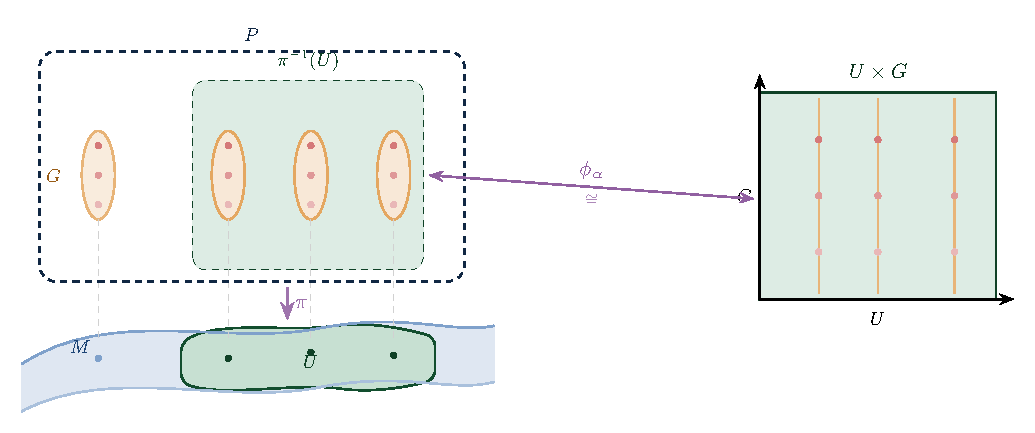
\includegraphics[width=0.7\textwidth]{images/fiber_bundle.pdf}
\caption[Estructura de un fibrado principal]{Estructura de un fibrado principal. El espacio total $P$ se proyecta sobre la variedad base $\mathcal{M}$ mediante $\pi$. Cada fibra $\pi^{-1}(x)$ es difeomorfa al grupo estructural $G$, y trivializaciones locales $\phi_\alpha$ permiten representar el fibrado como productos $U_\alpha \times G$ en regiones abiertas.}
\label{fig:fiber_bundle}
\end{figure}

\begin{example}[Fibrado de Marcos Ortonormales]\label{ex:fibrado_marcos}
Sea $(\mathcal{M}, g)$ una variedad Riemanniana $n$-dimensional. El \textit{fibrado de marcos ortonormales} $\mathrm{FM}(\mathcal{M})$ es un fibrado principal $(P, \mathcal{M}, \pi, O(n))$ donde:
\begin{itemize}
    \item El espacio total $P$ consiste en todos los marcos ortonormales: $P = \{(p, e_1, \ldots, e_n) : p \in \mathcal{M}, \{e_i\} \text{ base ortonormal de } T_p\mathcal{M}\}$
    \item La proyección $\pi: P \to \mathcal{M}$ envía $(p, e_1, \ldots, e_n) \mapsto p$
    \item El grupo $O(n)$ actúa por la derecha: $(p, e_1, \ldots, e_n) \cdot A = (p, \sum_j A_{j1}e_j, \ldots, \sum_j A_{jn}e_j)$
\end{itemize}
Cada fibra $\pi^{-1}(p)$ es difeomorfa a $O(n)$ y representa todas las posibles elecciones de marco ortonormal en el punto $p$.
\end{example}

\begin{example}[Fibrado Trivial]\label{ex:fibrado_trivial}
El caso más simple es el \textit{fibrado trivial} $P = \mathcal{M} \times G$ con proyección $\pi(p, g) = p$ y acción $(p, h) \cdot g = (p, hg)$. Este fibrado admite una sección global $s: \mathcal{M} \to P$ dada por $s(p) = (p, e)$, donde $e$ es la identidad de $G$. No todos los fibrados principales admiten secciones globales; la existencia de tales secciones está relacionada con la topología del espacio base.
\end{example}

En el contexto del \gls{GDL}, el espacio base $\mathcal{M}$ representa el dominio donde viven los datos (por ejemplo, la esfera $S^2$ para datos esféricos), mientras que el grupo $G$ codifica las simetrías locales relevantes (por ejemplo, $SO(2)$ para rotaciones en el plano tangente). La fibra sobre cada punto contiene todas las posibles ``orientaciones locales'' o ``marcos de referencia'' en ese punto.

\subsection{Conexiones en Fibrados Principales}\label{subsec:conexiones_fibrados}

Una conexión en un fibrado principal proporciona una manera de ``transportar'' información entre fibras diferentes de forma consistente con la estructura del grupo. Matemáticamente, una conexión especifica una descomposición del espacio tangente al fibrado en componentes ``horizontales'' y ``verticales''.

\begin{definition}[Espacio Vertical]\label{def:espacio_vertical}
Sea $(P, \mathcal{M}, \pi, G)$ un fibrado principal. Para cada $u \in P$, el \textit{espacio vertical} $V_u P$ es el subespacio de $T_u P$ tangente a la fibra:
\[
V_u P = \ker(d\pi_u) = \{X \in T_u P : d\pi_u(X) = 0\}
\]
\end{definition}

\begin{definition}[Campo Vectorial Fundamental]\label{def:campo_vectorial_fundamental}
Sea $(P, \mathcal{M}, \pi, G)$ un fibrado principal. Para cada $A \in \mathfrak{g}$ (\autoref{def:algebra_lie}) y cada $u \in P$, el \textit{campo vectorial fundamental} generado por $A$ en $u$ es:
\[
A^*_u = \frac{d}{dt}\bigg|_{t=0} u \cdot \exp(tA)
\]
donde $\exp: \mathfrak{g} \to G$ es el mapa exponencial (\autoref{def:mapa_exponencial}). La curva $t \mapsto u \cdot \exp(tA)$ permanece enteramente en la fibra $\pi^{-1}(\pi(u))$, puesto que la acción de $G$ preserva fibras (condición (b) de la \autoref{def:fibrado_principal_formal}), de donde $A^*_u \in V_u P$.
\end{definition}

\begin{proposition}[Isomorfismo Canónico $V_u P \cong \mathfrak{g}$]\label{prop:vertical_lie_isomorfismo}
Para cada $u \in P$, la aplicación $\sigma_u: \mathfrak{g} \to V_u P$ definida por $\sigma_u(A) = A^*_u$ es un isomorfismo de espacios vectoriales.
\end{proposition}

\begin{proof}
Consideremos la \textit{aplicación de órbita} $\Phi_u: G \to P$ definida por $\Phi_u(g) = u \cdot g$. Su diferencial en la identidad es $\sigma_u = (d\Phi_u)_e: T_eG = \mathfrak{g} \to T_uP$, cuya imagen está contenida en $V_uP$ por la \autoref{def:campo_vectorial_fundamental}.

\textbf{Linealidad.} Como diferencial de una aplicación suave, $\sigma_u = (d\Phi_u)_e$ es una aplicación lineal.

\textbf{Inyectividad.} Como la acción de $G$ es libre, $\Phi_u$ es inyectiva. Además, $\Phi_u$ es una inmersión (\autoref{def:inmersion_suave}): si $(d\Phi_u)_e(A) = 0$, la curva $t \mapsto u \cdot \exp(tA)$ tendría velocidad nula en $t = 0$, lo que por libertad de la acción implica $A = 0$. Luego $\sigma_u$ es inyectiva.

\textbf{Suryectividad.} Como $\pi$ es una submersión (\autoref{def:submersion_suave}), $d\pi_u$ es suryectiva y $\dim V_u P = \dim \ker(d\pi_u) = \dim P - \dim \mathcal{M} = \dim G = \dim \mathfrak{g}$. Un mapa lineal inyectivo entre espacios de igual dimensión finita es un isomorfismo.
\end{proof}

\begin{definition}[Conexión en Fibrado Principal]\label{def:conexion_fibrado}
Una \textit{conexión} en el fibrado principal $(P, \mathcal{M}, \pi, G)$ es una 1-forma (\autoref{def:1_forma_diferencial}) $\omega \in \Omega^1(P, \mathfrak{g})$ con valores en el álgebra de Lie $\mathfrak{g}$ de $G$ que satisface:
\begin{enumerate}
    \item \textbf{Normalización}: $\omega(A^*_u) = A$ para todo $A \in \mathfrak{g}$ y $u \in P$, donde $A^*$ es el campo vectorial fundamental generado por $A$
    \item \textbf{Equivarianza}: $R_g^* \omega = \mathrm{Ad}_{g^{-1}} \omega$ para todo $g \in G$, donde $R_g: P \to P$ denota la acción por la derecha y $\mathrm{Ad}$ es la representación adjunta
\end{enumerate}
Equivalentemente, una conexión determina una \textit{distribución horizontal} $H_u P = \ker(\omega_u) \subset T_u P$ complementaria al espacio vertical, tal que $T_u P = H_u P \oplus V_u P$ y $H_{u \cdot g} P = (R_g)_* H_u P$.

Para una exposición detallada, véase~\citep{Taubes2011}.
\end{definition}

\textbf{Interpretación Geométrica.} La distribución horizontal $H_u P$ especifica qué direcciones en el espacio total son ``puramente espaciales'' (paralelas a la base) versus ``puramente de gauge'' (a lo largo de la fibra). Una curva $\tilde{\gamma}$ en $P$ es \textit{horizontal} si $\dot{\tilde{\gamma}}(t) \in H_{\tilde{\gamma}(t)} P$ para todo $t$; tales curvas representan transporte ``sin rotación'' del marco de referencia.

\subsection{Transporte Paralelo}\label{subsec:transporte_paralelo_gdl}

El transporte paralelo es el mecanismo que permite comparar objetos (vectores, tensores, o más generalmente elementos del fibrado) situados en diferentes puntos de la variedad base. Esta comparación es esencial para definir operaciones como la convolución en variedades no euclidianas.

\begin{definition}[Transporte Paralelo en Fibrados Principales]\label{def:transporte_paralelo_formal}
Sea $(P, \mathcal{M}, \pi, G)$ un fibrado principal con conexión $\omega$. Para un camino suave $\gamma: [0,1] \to \mathcal{M}$, el \textit{transporte paralelo} a lo largo de $\gamma$ es la aplicación
\[
\Gamma_\gamma: \pi^{-1}(\gamma(0)) \to \pi^{-1}(\gamma(1))
\]
definida como sigue: dado $u_0 \in \pi^{-1}(\gamma(0))$, existe un único \textit{levantamiento horizontal} $\tilde{\gamma}: [0,1] \to P$ tal que:
\begin{enumerate}
    \item $\pi \circ \tilde{\gamma} = \gamma$ (el levantamiento proyecta sobre $\gamma$)
    \item $\tilde{\gamma}(0) = u_0$ (condición inicial)
    \item $\dot{\tilde{\gamma}}(t) \in H_{\tilde{\gamma}(t)} P$ para todo $t$ (horizontalidad)
\end{enumerate}
Entonces $\Gamma_\gamma(u_0) = \tilde{\gamma}(1)$.
\end{definition}

\begin{theorem}[Propiedades del Transporte Paralelo]\label{thm:propiedades_transporte}
El transporte paralelo satisface las siguientes propiedades fundamentales:
\begin{enumerate}
    \item \textbf{Equivarianza}: $\Gamma_\gamma(u \cdot g) = \Gamma_\gamma(u) \cdot g$ para todo $g \in G$
    \item \textbf{Composición}: $\Gamma_{\gamma_2 * \gamma_1} = \Gamma_{\gamma_2} \circ \Gamma_{\gamma_1}$, donde $\gamma_2 * \gamma_1$ denota la concatenación de caminos
    \item \textbf{Inversión}: $\Gamma_{\gamma^{-1}} = (\Gamma_\gamma)^{-1}$, donde $\gamma^{-1}(t) = \gamma(1-t)$
\end{enumerate}
\end{theorem}

\begin{proof}
\textbf{Equivarianza.} Sea $\tilde{\gamma}$ el levantamiento horizontal de $\gamma$ con $\tilde{\gamma}(0) = u$, y definamos $\tilde{\gamma}_g(t) = \tilde{\gamma}(t) \cdot g$. Verificamos las tres condiciones de la \autoref{def:transporte_paralelo_formal}:
\begin{enumerate}
    \item \textbf{Proyección}: como la acción de $G$ preserva fibras, $\pi(\tilde{\gamma}_g(t)) = \pi(\tilde{\gamma}(t)) = \gamma(t)$.
    \item \textbf{Condición inicial}: $\tilde{\gamma}_g(0) = \tilde{\gamma}(0) \cdot g = u \cdot g$.
    \item \textbf{Horizontalidad}: $\dot{\tilde{\gamma}}_g(t) = (R_g)_* \dot{\tilde{\gamma}}(t) \in (R_g)_* H_{\tilde{\gamma}(t)} P = H_{\tilde{\gamma}(t) \cdot g} P$, donde la última igualdad usa la $G$-invariancia de la distribución horizontal (\autoref{def:conexion_fibrado}).
\end{enumerate}
Por unicidad del levantamiento horizontal, $\tilde{\gamma}_g$ es el levantamiento de $\gamma$ desde $u \cdot g$, luego $\Gamma_\gamma(u \cdot g) = \tilde{\gamma}_g(1) = \tilde{\gamma}(1) \cdot g = \Gamma_\gamma(u) \cdot g$.

\textbf{Composición.} Sea $\tilde{\gamma}_1$ el levantamiento horizontal de $\gamma_1$ desde $u_0$, con punto final $u_1 = \tilde{\gamma}_1(1)$, y sea $\tilde{\gamma}_2$ el levantamiento horizontal de $\gamma_2$ desde $u_1$. La curva concatenada
\[
\tilde{\gamma}(t) = \begin{cases} \tilde{\gamma}_1(2t), & t \in [0, \tfrac{1}{2}], \\ \tilde{\gamma}_2(2t - 1), & t \in [\tfrac{1}{2}, 1], \end{cases}
\]
satisface: proyecta sobre $\gamma_2 * \gamma_1$, parte de $u_0$ y es horizontal en cada tramo. Por unicidad, es el levantamiento horizontal de $\gamma_2 * \gamma_1$ desde $u_0$, y su punto final es $\tilde{\gamma}_2(1) = \Gamma_{\gamma_2}(\Gamma_{\gamma_1}(u_0))$.

\textbf{Inversión.} Sea $\tilde{\gamma}$ el levantamiento horizontal de $\gamma$ desde $u_0$ con punto final $u_1 = \tilde{\gamma}(1)$. Definamos $\tilde{\gamma}^{-}(t) = \tilde{\gamma}(1-t)$. Entonces: $\pi(\tilde{\gamma}^{-}(t)) = \gamma(1-t) = \gamma^{-1}(t)$; $\tilde{\gamma}^{-}(0) = u_1$; y $\dot{\tilde{\gamma}}^{-}(t) = -\dot{\tilde{\gamma}}(1-t) \in H_{\tilde{\gamma}(1-t)}P$, pues los subespacios horizontales son espacios vectoriales. Por unicidad, $\tilde{\gamma}^{-}$ es el levantamiento de $\gamma^{-1}$ desde $u_1$, luego $\Gamma_{\gamma^{-1}}(u_1) = \tilde{\gamma}^{-}(1) = u_0 = \Gamma_\gamma^{-1}(u_1)$.

Para una exposición alternativa, véase~\citep[Cap.~II, Prop.~3.2]{Kobayashi1996}.
\end{proof}

\begin{figure}[htbp]
\centering
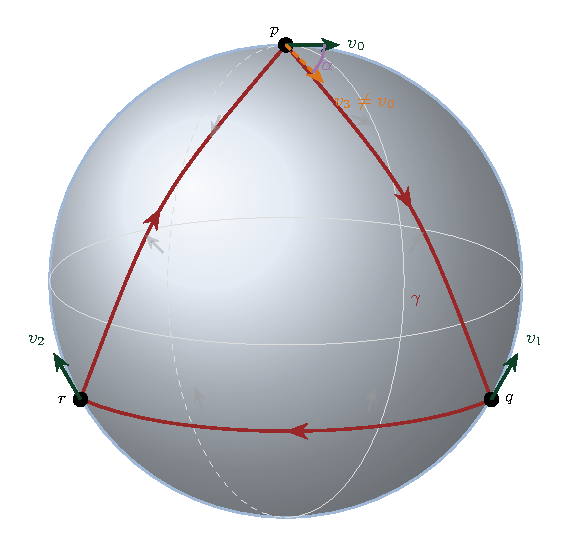
\includegraphics[width=0.85\textwidth]{images/parallel_transport.pdf}
\caption[Transporte paralelo y holonomía]{Transporte paralelo a lo largo de una curva $\gamma$ en una variedad. Un vector tangente en $\gamma(0)$ se transporta a lo largo del camino manteniéndose ``paralelo'' según la conexión. La holonomía surge cuando el vector retorna a su punto inicial tras recorrer un lazo cerrado.}
\label{fig:parallel_transport}
\end{figure}

\textbf{Ecuación Diferencial del Transporte.} En términos de la forma de conexión, el levantamiento horizontal $\tilde{\gamma}$ satisface la ecuación diferencial:
\[
\omega(\dot{\tilde{\gamma}}(t)) = 0
\]
Si expresamos $\tilde{\gamma}(t) = \tilde{\gamma}_0(t) \cdot g(t)$ donde $\tilde{\gamma}_0$ es una sección local y $g: [0,1] \to G$, entonces $g(t)$ satisface:
\[
\frac{dg}{dt} + \omega(\dot{\gamma}(t)) g(t) = 0
\]
con solución formal $g(1) = \mathcal{P} \exp\left(-\int_0^1 \omega(\dot{\gamma}(t)) dt\right) g(0)$, donde $\mathcal{P}$ denota el ordenamiento de camino (path ordering).

\subsection{Curvatura y Ecuación de Estructura}\label{subsec:curvatura_estructura}

La curvatura de una conexión mide la obstrucción a la integrabilidad de la distribución horizontal, o equivalentemente, cuánto depende el transporte paralelo del camino elegido entre dos puntos.

\begin{definition}[Curvatura de Conexión]\label{def:curvatura_formal}
Sea $\omega$ una conexión en el fibrado principal $(P, \mathcal{M}, \pi, G)$. La \textit{curvatura} $\Omega_\omega$ es la 2-forma con valores en $\mathfrak{g}$ definida mediante la derivada exterior (\autoref{def:derivada_exterior}) y el producto exterior (\autoref{def:producto_exterior_k_formas}) por:
\begin{equation}\label{eq:curvatura_definicion}
\Omega_\omega = d\omega + \frac{1}{2}[\omega \wedge \omega]
\end{equation}
donde $[\omega \wedge \omega](X, Y) = [\omega(X), \omega(Y)]$ utiliza el corchete de Lie en $\mathfrak{g}$.

En forma más explícita, para campos vectoriales $X, Y$ en $P$:
\[
\Omega_\omega(X, Y) = d\omega(X, Y) + [\omega(X), \omega(Y)]
\]
La curvatura es una 2-forma horizontal y equivariante~\citep{Chern2000}.
\end{definition}

\begin{theorem}[Ecuación de Estructura de Cartan]\label{thm:cartan_estructura}
La curvatura $\Omega_\omega$ y la conexión $\omega$ satisfacen la \textit{ecuación de estructura de Cartan}:
\begin{equation}\label{eq:estructura_cartan}
d\omega = \Omega_\omega - \frac{1}{2}[\omega \wedge \omega]
\end{equation}
Además, la curvatura satisface la \textit{identidad de Bianchi}:
\begin{equation}\label{eq:bianchi}
d\Omega_\omega = [\omega \wedge \Omega_\omega]
\end{equation}
\end{theorem}

\begin{proof}
La ecuación de estructura es simplemente un reordenamiento de la definición de curvatura. Para la identidad de Bianchi, aplicamos $d$ a ambos lados de \eqref{eq:curvatura_definicion}:
\[
d\Omega_\omega = d(d\omega) + \frac{1}{2}d[\omega \wedge \omega] = \frac{1}{2}([d\omega \wedge \omega] - [\omega \wedge d\omega])
\]
Sustituyendo $d\omega = \Omega_\omega - \frac{1}{2}[\omega \wedge \omega]$ y usando las propiedades del corchete de Lie (identidad de Jacobi), se obtiene $d\Omega_\omega = [\omega \wedge \Omega_\omega]$.
\end{proof}

\begin{definition}[Holonomía]\label{def:holonomia}
Sea $\gamma: [0,1] \to \mathcal{M}$ un lazo cerrado basado en $p$ (es decir, $\gamma(0) = \gamma(1) = p$). La \textit{holonomía} de la conexión $\omega$ a lo largo de $\gamma$ es el elemento $g_\gamma \in G$ tal que:
\[
\Gamma_\gamma(u) = u \cdot g_\gamma
\]
para cualquier $u \in \pi^{-1}(p)$.

El \textit{grupo de holonomía} $\mathrm{Hol}_p(\omega)$ es el subgrupo de $G$ generado por las holonomías de todos los lazos basados en $p$.
\end{definition}

\textbf{Curvatura como Holonomía Infinitesimal.} La curvatura puede interpretarse como la ``holonomía infinitesimal'': para un lazo infinitesimal que encierra un área $dA$ en la variedad base, la holonomía es aproximadamente $\exp(\Omega_\omega \cdot dA)$. Si la curvatura es nula ($\Omega_\omega = 0$), la conexión es \textit{plana} y el transporte paralelo es independiente del camino (para caminos homotópicos).

\subsection{Invarianza Gauge en Redes Neuronales}\label{subsec:invarianza_gauge_redes}

Los conceptos anteriores tienen implicaciones directas para el diseño de arquitecturas neuronales equivariantes. Las arquitecturas geométricas modernas deben respetar invarianzas gauge para garantizar que las predicciones no dependan de elecciones arbitrarias de coordenadas o marcos de referencia.

\begin{definition}[Transformación Gauge]\label{def:transformacion_gauge}
Una \textit{transformación gauge} es una aplicación suave $g: \mathcal{M} \to G$ que asigna a cada punto $p \in \mathcal{M}$ un elemento $g(p)$ del grupo estructural. El conjunto de todas las transformaciones gauge forma el \textit{grupo gauge}:
\[
\mathcal{G} = C^\infty(\mathcal{M}, G)
\]
con la operación de multiplicación punto a punto: $(g_1 \cdot g_2)(p) = g_1(p) \cdot g_2(p)$.
\end{definition}

\begin{definition}[Función Gauge Equivariante]\label{def:funcion_gauge_equivariante_gdl}
Sea $\rho: G \to GL(V)$ una representación de $G$ en un espacio vectorial $V$. Una función $f: P \to V$ sobre el fibrado principal es \textit{gauge equivariante} (o de tipo $\rho$) si:
\begin{equation}
f(u \cdot g) = \rho(g^{-1}) f(u)
\end{equation}
para todo $u \in P$ y $g \in G$.
\end{definition}

\begin{figure}[htbp]
\centering
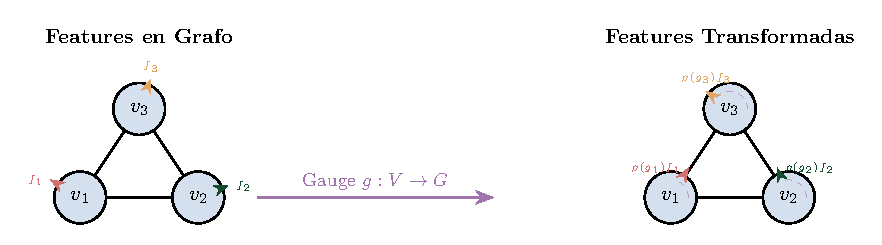
\includegraphics[width=0.75\textwidth]{images/gauge_transformation.pdf}
\caption[Transformación gauge en un grafo]{Transformación gauge en un grafo. Una transformación gauge $g: V \to G$ rota independientemente el marco de referencia en cada vértice, transformando las features $f_i$ en $\rho(g_i)f_i$. Los arcos punteados indican la rotación local aplicada en cada nodo.}
\label{fig:gauge_transformation}
\end{figure}

Las transformaciones gauge actúan sobre las funciones del fibrado, y una arquitectura neuronal $\Phi$ es gauge equivariante si conmuta con esta acción. Formalmente, si la salida es un escalar (predicción global), la red es \textit{gauge invariante}:
\begin{equation}\label{eq:gauge_invariance_network}
\Phi(g \cdot f) = \Phi(f) \quad \text{para todo } g: V \to G
\end{equation}
Esto garantiza que:

\begin{itemize}
    \item \textbf{Redes en grafos}: La salida es invariante bajo reordenamiento de nodos (gauge permutacional)
    \item \textbf{Redes en variedades}: Las predicciones son independientes de la parametrización o carta local elegida
    \item \textbf{Redes equivariantes}: Las características se transforman coherentemente bajo cambios de marco de referencia local
\end{itemize}

\textbf{Conexión con Física Teórica.} La teoría gauge en \gls{GDL} es análoga a las teorías gauge en física, donde las fuerzas fundamentales (electromagnetismo, fuerza débil, fuerza fuerte) se describen mediante conexiones en fibrados principales con grupos $U(1)$, $SU(2)$ y $SU(3)$ respectivamente. En \gls{GDL}, el grupo gauge codifica las simetrías locales relevantes para el problema de aprendizaje.

La implementación práctica de estas ideas en arquitecturas neuronales concretas, incluyendo las Gauge Equivariant CNNs, se desarrolla en detalle en la \autoref{sec:gauge_cnns} del \autoref{ch:cnn}.

\subsection{Ejemplos de Gauge Equivarianza en GDL}\label{subsec:ejemplos_gauge_gdl}

Para ilustrar la relevancia práctica de los conceptos de gauge equivarianza, presentamos ejemplos concretos de cómo estas ideas se manifiestan en aplicaciones de \gls{GDL}.

\begin{example}[Gauge Equivarianza en Mallas Trianguladas 3D]\label{ex:gauge_mallas_3d}
Consideremos una superficie 3D representada como una malla triangular $\mathcal{M} = (V, F)$, donde $V$ es el conjunto de vértices y $F$ el conjunto de caras triangulares. En cada vértice $v \in V$, el plano tangente $T_v\mathcal{M}$ está bien definido geométricamente, pero \textbf{no existe una elección canónica de base ortonormal} $(e_1^v, e_2^v)$ para este plano.

El problema de gauge surge cuando intentamos definir campos vectoriales o características direccionales sobre la malla:
\begin{itemize}
    \item \textbf{Elección de gauge}: Para cada vértice $v$, elegimos una base ortonormal $(e_1^v, e_2^v)$ del plano tangente. Esta elección es arbitraria: cualquier rotación $R_\theta \in SO(2)$ produce otra base igualmente válida.

    \item \textbf{Transformación gauge}: Si rotamos la base en el vértice $v$ por un ángulo $\theta_v$, las componentes de un vector $\mathbf{u} = u_1 e_1^v + u_2 e_2^v$ se transforman como:
    \begin{equation}
    \begin{pmatrix} u_1' \\ u_2' \end{pmatrix} = \begin{pmatrix} \cos\theta_v & \sin\theta_v \\ -\sin\theta_v & \cos\theta_v \end{pmatrix} \begin{pmatrix} u_1 \\ u_2 \end{pmatrix}
    \end{equation}

    \item \textbf{Requisito de gauge equivarianza}: Una red neuronal que procesa características vectoriales sobre la malla debe producir predicciones que sean \textbf{independientes} de la elección de bases locales. Matemáticamente, si $f: \mathcal{F}(\mathcal{M}) \to \mathcal{Y}$ es la función aprendida, debe satisfacer:
    \begin{equation}
    f(\rho(g) \cdot \mathbf{x}) = \rho'(g) \cdot f(\mathbf{x})
    \end{equation}
    donde $g = \{R_{\theta_v}\}_{v \in V}$ representa una transformación gauge (rotación independiente en cada vértice).
\end{itemize}
\end{example}

\begin{example}[Impacto de la Elección de Gauge en Predicciones]\label{ex:impacto_gauge_predicciones}
Para ilustrar por qué la gauge equivarianza es crucial, consideremos una red neuronal ingenua que procesa características vectoriales en mallas sin respetar invarianzas gauge.

\textbf{Problema:} Dada una superficie con un campo de curvatura principal, queremos predecir la dirección de máxima curvatura en cada punto.

\textbf{Arquitectura no gauge-equivariante:} Una \gls{MLP} que toma las componentes $(u_1, u_2)$ de vectores en coordenadas locales y predice las componentes de la dirección de curvatura.

\textbf{Fallo observado:} Si cambiamos la orientación del marco local en un vértice (una transformación gauge), las predicciones cambian de manera inconsistente:
\begin{itemize}
    \item Marco original: La red predice dirección $(\hat{d}_1, \hat{d}_2) = (0.8, 0.6)$
    \item Tras rotar el marco $45^\circ$: La red predice $(\hat{d}_1', \hat{d}_2') = (0.3, 0.9)$: ¡una dirección completamente diferente!
\end{itemize}

\textbf{Arquitectura gauge-equivariante:} Las redes como Gauge Equivariant Mesh CNNs~\citep{cohen2019gaugeequivariantconvolutional} utilizan convoluciones que transforman coherentemente bajo cambios de gauge. Sus predicciones satisfacen:
\begin{equation}
\hat{\mathbf{d}}' = R_\theta \hat{\mathbf{d}}
\end{equation}
donde $R_\theta$ es la misma rotación aplicada al marco local. Así, aunque las \textit{componentes numéricas} cambian, la \textit{dirección geométrica} predicha permanece invariante.
\end{example}

\begin{example}[Gauge Equivarianza para Moléculas 3D]\label{ex:gauge_moleculas}
En el modelado de moléculas tridimensionales, la gauge equivarianza se manifiesta de manera particularmente importante para arquitecturas que predicen propiedades tensoriales.

Consideremos una molécula con $n$ átomos en posiciones $\{\mathbf{r}_i\}_{i=1}^n \subset \mathbb{R}^3$. Queremos predecir el \textbf{tensor de polarizabilidad} $\boldsymbol{\alpha} \in \mathbb{R}^{3 \times 3}$, que describe cómo responde la distribución electrónica a campos eléctricos externos.

\textbf{Propiedad física fundamental:} Si rotamos la molécula por $R \in SO(3)$, el tensor de polarizabilidad se transforma como:
\begin{equation}
\boldsymbol{\alpha}' = R \boldsymbol{\alpha} R^T
\end{equation}
Esta es una transformación de tipo tensor de orden 2 bajo el grupo $SO(3)$.

\textbf{Arquitecturas gauge equivariantes:} Redes como NequIP~\citep{batzner2022nequip} y Allegro representan características intermedias mediante \textbf{tensores esféricos}, que transforman según representaciones irreducibles de $SO(3)$. El tensor de polarizabilidad se construye mediante productos tensoriales equivariantes:
\begin{equation}
\boldsymbol{\alpha} = \sum_{\ell=0,2} W_\ell \left( \mathbf{Y}^{(\ell)} \otimes \mathbf{Y}^{(\ell)} \right)
\end{equation}
donde $\mathbf{Y}^{(\ell)}$ son armónicos esféricos de orden $\ell$ y $W_\ell$ son pesos aprendidos. Esta construcción garantiza automáticamente la transformación correcta bajo rotaciones.

\textbf{Ventaja práctica:} Las predicciones son físicamente consistentes independientemente de la orientación arbitraria de la molécula en el espacio, eliminando la necesidad de aumentación de datos por rotaciones y mejorando significativamente la eficiencia del entrenamiento.
\end{example}

\textbf{Síntesis de los ejemplos.} Los tres ejemplos anteriores ilustran un principio común: cuando los datos tienen simetrías locales (libertades de gauge), las arquitecturas neuronales deben respetar estas simetrías para producir predicciones físicamente significativas. La teoría de fibrados principales proporciona el marco matemático riguroso para entender y diseñar tales arquitecturas.


\section{Síntesis: El Marco Unificador del GDL}\label{sec:sintesis_marco_unificador}

Las cinco G's fundamentales del \gls{GDL} (Geometría, Grupos, Grafos, Geodésicas y Gauges) forman un marco conceptual profundamente interconectado: la \textbf{Geometría} determina la estructura del dominio y define qué \textbf{Grupos} de simetrías son naturales; los \textbf{Grafos} discretizan las geometrías continuas preservando propiedades topológicas y espectrales; las \textbf{Geodésicas} definen caminos óptimos que respetan la geometría; y los \textbf{Gauges} aseguran que las representaciones sean intrínsecas. Desde esta perspectiva, las diferencias entre arquitecturas neuronales reflejan elecciones sobre tres aspectos geométricos: la \textbf{estructura del dominio} (espacios euclidianos, grafos, variedades), el \textbf{grupo de simetrías} (trivial, traslaciones, permutaciones) y la \textbf{conectividad} (global, vecindarios fijos, adaptativa). Las \glspl{ANN} tradicionales, operando en $\mathbb{R}^d$ con simetrías triviales (\autoref{ch:neural_networks}), constituyen el caso base: no explotan estructura geométrica alguna, de modo que toda invarianza debe aprenderse desde los datos. El \gls{GDL} resuelve esto incorporando las simetrías directamente en la arquitectura mediante el principio de equivarianza (\autoref{subsec:equivarianza_invarianza}).

\subsection{Message Passing: El Marco Unificador}\label{subsec:message_passing_unificador}

Las \textbf{Message Passing Neural Networks} (\glspl{MPNN}) proporcionan el marco matemático unificador que subyace a todas las arquitecturas de \gls{GDL}. Su fundamento conceptual radica en la estructura de grafos introducida en la \autoref{def:grafo_neuronal} del \autoref{ch:neural_networks} y la \autoref{def:vecindad_grafo} de la \autoref{sec:grafos_discretizacion}, donde los datos se organizan como nodos conectados por aristas que codifican relaciones estructurales.

Esta perspectiva revela que las diferencias aparentes entre \glspl{ANN}, \glspl{CNN}, \glspl{Transformer} y \glspl{GNN} son manifestaciones de diferentes topologías de grafos y estrategias de conectividad sobre el mismo paradigma fundamental: la propagación de información a través de vecindarios estructurados.

\begin{definition}[Red Neuronal de Paso de Mensajes]\label{def:mpnn_unificador}
Una \textit{\gls{MPNN}} opera sobre un grafo $\mathcal{G} = (V, E)$ con características de nodos $\{h_v\}_{v \in V}$ y aristas $\{e_{uv}\}_{(u,v) \in E}$. La actualización en la capa $\ell$ consta de dos fases:

\begin{enumerate}
    \item \textbf{Paso de Mensajes}:
    \begin{equation}
    m_v^{(\ell+1)} = \sum_{u \in \mathcal{N}(v)} M_\ell(h_v^{(\ell)}, h_u^{(\ell)}, e_{vu})
    \end{equation}
      \item \textbf{Actualización de Nodo}:
    \begin{equation}
    h_v^{(\ell+1)} = U_\ell(h_v^{(\ell)}, m_v^{(\ell+1)})
    \end{equation}
\end{enumerate}

donde $M_\ell$ es la función de mensaje, $U_\ell$ es la función de actualización, y $\mathcal{N}(v)$ es el vecindario del nodo $v$ (\autoref{def:vecindad_grafo}). Esta formulación generaliza naturalmente las estructuras de datos discretas. Nótese que este esquema opera exclusivamente sobre nodos y aristas; su generalización a $k$-símplices de orden superior, el \textit{paso de mensajes simplicial}, se desarrolla en la \autoref{subsubsec:tdl_mpnn_general}.
\end{definition}

\begin{figure}[htbp]
\centering
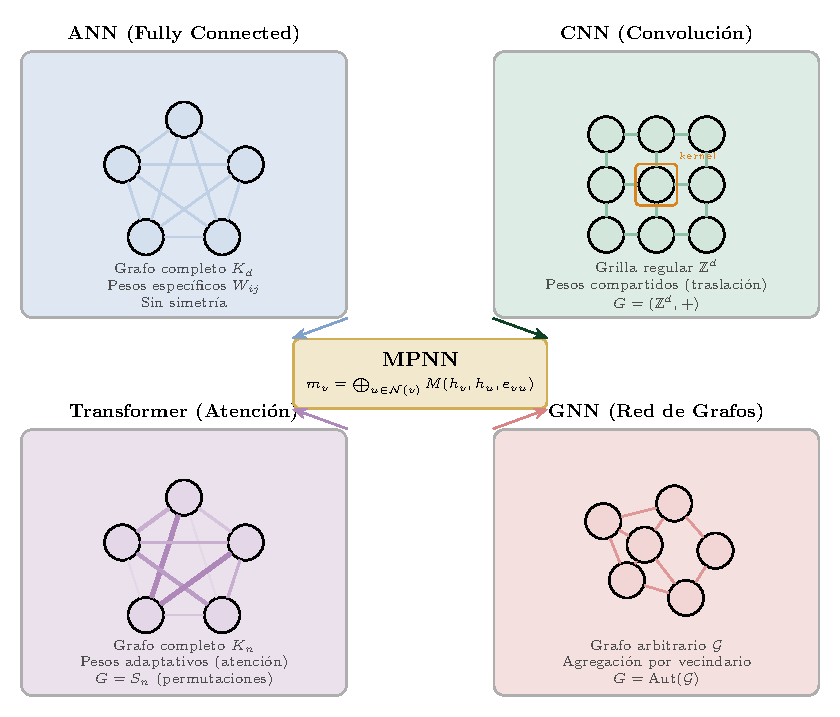
\includegraphics[width=\textwidth]{images/mpnn_unification.pdf}
\caption[Unificación de arquitecturas mediante Message Passing]{Las cuatro arquitecturas principales del Deep Learning como instancias del marco \gls{MPNN}. \textbf{ANN}: grafo completo con pesos específicos para cada par. \textbf{CNN}: grilla regular con pesos compartidos por traslación. \textbf{Transformer}: grafo completo con pesos adaptativos (atención). \textbf{GNN}: grafo arbitrario con agregación por vecindario. Las diferencias residen en la topología del grafo y el grupo de simetría $G$.}
\label{fig:mpnn_unification}
\end{figure}

\subsubsection{ANNs como MPNNs Triviales}

Las \glspl{ANN} tradicionales pueden interpretarse como el caso más simple de \glspl{MPNN}, donde cada nodo se conecta con todos los demás con pesos uniformes:

\begin{proposition}[\gls{ANN} como \gls{MPNN} sobre grafo completo uniforme]\label{prop:ann_mpnn}
Una capa completamente conectada $h^{(\ell+1)} = \sigma(W h^{(\ell)} + b)$ es equivalente a una \gls{MPNN} donde:
\begin{itemize}
    \item \textbf{Grafo}: Grafo completo $K_d$ donde cada característica es un nodo
    \item \textbf{Mensaje}: $M(h_v, h_u, e_{vu}) = W_{vu} h_u$ (peso específico para cada par)
    \item \textbf{Agregación}: Suma sobre todas las características de entrada
    \item \textbf{Actualización}: $U(h_v, m_v) = \sigma(m_v + b_v)$
\end{itemize}
\end{proposition}

\begin{proof}
Sea $h^{(\ell)} \in \mathbb{R}^d$ el vector de características en la capa $\ell$. La capa completamente conectada calcula:
\[
h_v^{(\ell+1)} = \sigma\!\left(\sum_{u=1}^{d} W_{vu} h_u^{(\ell)} + b_v\right)
\]
Interpretando cada componente como un nodo del grafo completo $K_d$, esta expresión coincide exactamente con el paso de mensajes (\autoref{def:mpnn_unificador}) con mensaje $M(h_v, h_u, e_{vu}) = W_{vu} h_u^{(\ell)}$, agregación $m_v = \sum_{u \in \mathcal{N}(v)} M(\cdot) = \sum_{u=1}^d W_{vu} h_u^{(\ell)}$, y actualización $U(h_v, m_v) = \sigma(m_v + b_v)$.
\end{proof}

Esta perspectiva revela por qué las \glspl{ANN} carecen de \textbf{bias inductivo geométrico}: tratan todas las conexiones entre características como igualmente importantes, ignorando cualquier estructura espacial, topológica o de similaridad que pueda existir en los datos.

\subsubsection{Convoluciones como Paso de Mensajes Regular}

Las \glspl{CNN} constituyen el primer caso no trivial de paso de mensajes, donde la estructura de la grilla impone un bias inductivo geométrico fundamental: la equivarianza traslacional.

\begin{proposition}[\gls{CNN} como \gls{MPNN} sobre grilla regular]\label{prop:cnn_mpnn}
Una capa convolucional sobre una grilla regular $\mathbb{Z}^d$ con kernel de soporte $\mathcal{K}$ es equivalente a una \gls{MPNN} donde:
\begin{itemize}
    \item \textbf{Grafo}: Grilla regular $\mathbb{Z}^d$ con aristas $\mathcal{N}(v) = \{u \in \mathbb{Z}^d : v - u \in \mathcal{K}\}$
    \item \textbf{Mensaje}: $M(h_v, h_u, e_{vu}) = W_{v-u} h_u$ (pesos compartidos por posición relativa)
    \item \textbf{Agregación}: Suma sobre el vecindario local $m_v = \sum_{u \in \mathcal{N}(v)} W_{v-u} h_u$
    \item \textbf{Actualización}: $U(h_v, m_v) = \sigma(m_v + b)$
\end{itemize}
\end{proposition}

\begin{proof}
Sea $h^{(\ell)}: \mathbb{Z}^d \to \mathbb{R}^{c_{\mathrm{in}}}$ la señal en la capa $\ell$ y $\{W_\delta\}_{\delta \in \mathcal{K}}$ el kernel convolucional con $W_\delta \in \mathbb{R}^{c_{\mathrm{out}} \times c_{\mathrm{in}}}$. La convolución discreta (\autoref{def:convolucion_discreta}) calcula:
\[
h_v^{(\ell+1)} = \sigma\!\left(\sum_{\delta \in \mathcal{K}} W_\delta\, h_{v-\delta}^{(\ell)} + b\right) = \sigma\!\left(\sum_{u \in \mathcal{N}(v)} W_{v-u}\, h_u^{(\ell)} + b\right)
\]
donde el cambio de variable $u = v - \delta$ transforma la suma sobre desplazamientos del kernel en una suma sobre vecinos del grafo de la grilla. Esta expresión coincide con el paso de mensajes (\autoref{def:mpnn_unificador}) con mensaje $M(h_v, h_u, e_{vu}) = W_{v-u} h_u^{(\ell)}$, agregación $m_v = \sum_{u \in \mathcal{N}(v)} M(\cdot)$ y actualización $U(h_v, m_v) = \sigma(m_v + b)$. La equivalencia constructiva completa, incluyendo la correspondencia capa a capa por inducción, se establece en el \autoref{thm:equivalencia_constructiva_cnn_gnn}.
\end{proof}

La diferencia clave respecto a las \glspl{ANN} es que los pesos $W_{v-u}$ dependen exclusivamente de la posición relativa, no del par absoluto $(v, u)$. Esta compartición de pesos (weight sharing) es precisamente la implementación de la equivarianza traslacional como bias inductivo geométrico (\autoref{theorem:convolution_translation_equivariance}), reduciendo drásticamente el número de parámetros de $O(n^2 c^2)$ a $O(|\mathcal{K}| c^2)$.

\subsubsection{Atención como Paso de Mensajes Adaptativo}

Los \glspl{Transformer} representan el caso complementario: los pesos de comunicación se calculan dinámicamente a partir del contenido de los nodos, no de su posición.

\begin{proposition}[\gls{Transformer} como \gls{MPNN} sobre grafo completo adaptativo]\label{prop:attention_mpnn}
Una capa de self-attention (\autoref{def:self_attention_basica}) sobre una secuencia de $n$ tokens es equivalente a una \gls{MPNN} donde:
\begin{itemize}
    \item \textbf{Grafo}: Grafo completo $K_n$ donde cada token es un nodo
    \item \textbf{Mensaje}: $M(h_i, h_j) = \alpha_{ij}\, V h_j$, con coeficientes de atención
    \[
    \alpha_{ij} = \frac{\exp\!\left(\frac{(Qh_i)^T(Kh_j)}{\sqrt{d_k}}\right)}{\sum_{m=1}^n \exp\!\left(\frac{(Qh_i)^T(Kh_m)}{\sqrt{d_k}}\right)}
    \]
    \item \textbf{Agregación}: Suma ponderada $m_i = \sum_{j=1}^n M(h_i, h_j)$
    \item \textbf{Actualización}: $U(h_i, m_i) = m_i$
\end{itemize}
\end{proposition}

\begin{proof}
Sea $\{h_1, \ldots, h_n\} \subset \mathbb{R}^d$ la secuencia de entrada y $Q, K, V \in \mathbb{R}^{d \times d_k}$ las matrices de proyección. La capa de self-attention (\autoref{def:self_attention_basica}) calcula:
\[
h_i^{(\ell+1)} = \sum_{j=1}^n \alpha_{ij}\, V h_j^{(\ell)}
= \sum_{j=1}^n \underbrace{\alpha_{ij}\, V h_j^{(\ell)}}_{M(h_i, h_j)}
\]
Identificando el grafo completo $K_n$ con $\mathcal{N}(i) = \{1, \ldots, n\}$, esta expresión es exactamente el paso de mensajes (\autoref{def:mpnn_unificador}) con mensaje $M(h_i, h_j) = \alpha_{ij} V h_j$ y actualización identidad $U(h_i, m_i) = m_i$. La normalización softmax garantiza $\alpha_{ij} \in (0,1)$ con $\sum_{j=1}^n \alpha_{ij} = 1$, de modo que la agregación es una combinación convexa, a diferencia de la suma uniforme de las \glspl{ANN} (\autoref{prop:ann_mpnn}) y las \glspl{CNN} (\autoref{prop:cnn_mpnn}).
\end{proof}

La diferencia fundamental respecto a las arquitecturas anteriores es que los pesos $\alpha_{ij}$ son funciones del contenido $(h_i, h_j)$, no fijos (\glspl{ANN}) ni dependientes de la posición relativa (\glspl{CNN}). Esta adaptabilidad permite conectividad global a costa de complejidad cuadrática $O(n^2)$ en la longitud de secuencia. El \autoref{ch:attention} desarrolla las extensiones geométricas de este mecanismo.

\subsubsection{TDL como Paso de Mensajes de Orden Superior}\label{subsubsec:tdl_mpnn_general}

Las tres arquitecturas anteriores (\glspl{ANN}, \glspl{CNN} y \glspl{Transformer}) operan exclusivamente sobre \textbf{nodos} ($0$-símplices) de un grafo, propagando información a lo largo de aristas. El \gls{TDL} rompe esta restricción: asigna señales a $k$-símplices de orden arbitrario y propaga información simultáneamente a través de las adyacencias inferior y superior definidas por los operadores de frontera. Esta extensión incorpora un \textbf{bias inductivo topológico} que captura relaciones de orden superior inaccesibles al paso de mensajes estándar.

\begin{definition}[Señal simplicial]\label{def:senal_simplicial_gdl}
	Una \textit{señal simplicial de orden $k$} sobre un complejo simplicial $\mathcal{K}$ es una función $\mathbf{x}: \mathcal{K}_k \to \mathbb{R}^d$ que asigna un vector de características $\mathbf{x}_\sigma \in \mathbb{R}^d$ a cada $k$-símplice $\sigma \in \mathcal{K}_k$.
\end{definition}

\begin{definition}[Paso de mensajes simplicial]\label{def:mensaje_simplicial_gdl}
	El \textit{paso de mensajes simplicial} generaliza el paso de mensajes en grafos (\autoref{def:mpnn_unificador}) mediante tres tipos de comunicación para cada $k$-símplice $\sigma$:
	\begin{enumerate}
		\item \textbf{Mensaje inferior} (vía $\partial_k^T$): Información de $(k{-}1)$-símplices en la frontera de $\sigma$:
		\[
			\mathbf{m}_\sigma^{\mathrm{down}} = \bigoplus_{\tau \in \mathcal{B}^{\mathrm{down}}(\sigma)} M^{\mathrm{down}}\!\left(\mathbf{h}_\sigma, \mathbf{h}_\tau\right)
		\]
		donde $\mathcal{B}^{\mathrm{down}}(\sigma) = \{\tau : [\partial_k^T \partial_k]_{\sigma,\tau} \neq 0\}$ son los $k$-símplices adyacentes por caras compartidas.

		\item \textbf{Mensaje superior} (vía $\partial_{k+1}$): Información de $(k{+}1)$-símplices que contienen a $\sigma$:
		\[
			\mathbf{m}_\sigma^{\mathrm{up}} = \bigoplus_{\rho \in \mathcal{B}^{\mathrm{up}}(\sigma)} M^{\mathrm{up}}\!\left(\mathbf{h}_\sigma, \mathbf{h}_\rho\right)
		\]
		donde $\mathcal{B}^{\mathrm{up}}(\sigma) = \{\rho : [\partial_{k+1} \partial_{k+1}^T]_{\sigma,\rho} \neq 0\}$ son los $k$-símplices que comparten un $(k{+}1)$-símplice.

		\item \textbf{Actualización}:
		\[
			\mathbf{h}_\sigma' = U\!\left(\mathbf{h}_\sigma, \mathbf{m}_\sigma^{\mathrm{down}}, \mathbf{m}_\sigma^{\mathrm{up}}\right)
		\]
	\end{enumerate}
	donde $\bigoplus$ denota una función de agregación (suma, media, máximo), $M^{\mathrm{down}}, M^{\mathrm{up}}$ son funciones de mensaje aprendibles, y $U$ es la función de actualización \citep{bodnar2021weisfeiler}.
\end{definition}

\begin{proposition}[\gls{TDL} como instancia generalizada del marco \gls{MPNN}]\label{prop:tdl_mpnn}
El paso de mensajes simplicial (\autoref{def:mensaje_simplicial_gdl}) es una instancia generalizada del marco \gls{MPNN} (\autoref{def:mpnn_unificador}) donde:
\begin{itemize}
    \item \textbf{Dominio}: Complejo simplicial $\mathcal{K}$, con los $k$-símplices $\sigma \in \mathcal{K}_k$ como ``nodos''
    \item \textbf{Vecindario}: Vecindario doble $\mathcal{N}(\sigma) = \mathcal{B}^{\mathrm{down}}(\sigma) \cup \mathcal{B}^{\mathrm{up}}(\sigma)$, determinado por los Laplacianos inferior $L_k^{\mathrm{down}} = \partial_k^T \partial_k$ y superior $L_k^{\mathrm{up}} = \partial_{k+1} \partial_{k+1}^T$
    \item \textbf{Mensaje}: Combinación de mensajes inferior y superior:
    \[
    M(\mathbf{h}_\sigma) = \left(\bigoplus_{\tau \in \mathcal{B}^{\mathrm{down}}(\sigma)} M^{\mathrm{down}}(\mathbf{h}_\sigma, \mathbf{h}_\tau),\; \bigoplus_{\rho \in \mathcal{B}^{\mathrm{up}}(\sigma)} M^{\mathrm{up}}(\mathbf{h}_\sigma, \mathbf{h}_\rho)\right)
    \]
    \item \textbf{Actualización}: $U(\mathbf{h}_\sigma, \mathbf{m}_\sigma^{\mathrm{down}}, \mathbf{m}_\sigma^{\mathrm{up}})$ aprendible
\end{itemize}
En particular, para $k=0$ se recupera el \gls{MPNN} estándar sobre grafos.
\end{proposition}

\begin{proof}
Verificamos la correspondencia con las tres componentes del marco \gls{MPNN}. Sea $\mathcal{K}$ un complejo simplicial y fijemos $k \geq 0$. Consideramos el grafo $\mathcal{G}_k = (\mathcal{K}_k, E_k)$ cuyos nodos son los $k$-símplices y cuyas aristas codifican la adyacencia dada por $L_k$:

\textbf{(1) Mensaje.} Para cada $k$-símplice $\sigma$, el paso de mensajes simplicial (\autoref{def:mensaje_simplicial_gdl}) calcula dos mensajes:
\[
\mathbf{m}_\sigma^{\mathrm{down}} = \bigoplus_{\tau \in \mathcal{B}^{\mathrm{down}}(\sigma)} M^{\mathrm{down}}(\mathbf{h}_\sigma, \mathbf{h}_\tau), \qquad
\mathbf{m}_\sigma^{\mathrm{up}} = \bigoplus_{\rho \in \mathcal{B}^{\mathrm{up}}(\sigma)} M^{\mathrm{up}}(\mathbf{h}_\sigma, \mathbf{h}_\rho)
\]
Definiendo $\mathcal{N}(\sigma) = \mathcal{B}^{\mathrm{down}}(\sigma) \cup \mathcal{B}^{\mathrm{up}}(\sigma)$ y el mensaje conjunto $\widetilde{M}(\mathbf{h}_\sigma, \mathbf{h}_\nu) = M^{\mathrm{down}}(\mathbf{h}_\sigma, \mathbf{h}_\nu)$ si $\nu \in \mathcal{B}^{\mathrm{down}}(\sigma)$ y $\widetilde{M}(\mathbf{h}_\sigma, \mathbf{h}_\nu) = M^{\mathrm{up}}(\mathbf{h}_\sigma, \mathbf{h}_\nu)$ si $\nu \in \mathcal{B}^{\mathrm{up}}(\sigma)$, esto adopta la forma $m_\sigma = \bigoplus_{\nu \in \mathcal{N}(\sigma)} \widetilde{M}(\mathbf{h}_\sigma, \mathbf{h}_\nu)$, que corresponde a la fase de mensaje de la \autoref{def:mpnn_unificador}.

\textbf{(2) Agregación.} El operador $\bigoplus$ (suma, media o máximo) desempeña el papel de la función de agregación permutación-invariante del esquema \gls{MPNN}.

\textbf{(3) Actualización.} La función $U(\mathbf{h}_\sigma, \mathbf{m}_\sigma^{\mathrm{down}}, \mathbf{m}_\sigma^{\mathrm{up}})$ corresponde directamente a la función de actualización $U_\ell$ del marco \gls{MPNN}.

\textbf{Reducción a $k=0$.} Para $0$-símplices (nodos), $\partial_0 = 0$ implica $L_0^{\mathrm{down}} = 0$, por lo que $\mathcal{B}^{\mathrm{down}}(v) = \emptyset$ y el mensaje inferior se anula. El mensaje superior se reduce a $\mathbf{m}_v^{\mathrm{up}} = \bigoplus_{u \in \mathcal{B}^{\mathrm{up}}(v)} M^{\mathrm{up}}(\mathbf{h}_v, \mathbf{h}_u)$, donde $\mathcal{B}^{\mathrm{up}}(v) = \{u : [\partial_1 \partial_1^T]_{vu} \neq 0\} = \mathcal{N}(v)$ es el vecindario estándar del nodo $v$ en el grafo $1$-esqueleto. Esto recupera exactamente el paso de mensajes clásico sobre grafos.
\end{proof}

\begin{proposition}[Expresividad del paso de mensajes simplicial]\label{prop:expresividad_simplicial}
	El paso de mensajes simplicial es estrictamente más expresivo que el paso de mensajes en grafos. Existen pares de complejos simpliciales no isomorfos cuyos 1-esqueletos son idénticos (y por tanto indistinguibles por \glspl{MPNN}), pero que las redes simpliciales distinguen correctamente gracias a la información topológica de orden superior.
\end{proposition}

Este resultado, demostrado por \citet{bodnar2021weisfeiler}, muestra que la información topológica codificada en los operadores de frontera $\partial_k$ proporciona un poder discriminativo que supera las limitaciones del test de \gls{WL} establecidas en la \autoref{subsubsec:test_weisfeiler_leman}.

Esta proposición cierra el arco de unificación del marco \gls{MPNN}: mientras las \glspl{ANN}, \glspl{CNN} y \glspl{Transformer} codifican \textit{bias} inductivos espaciales o relacionales sobre nodos, el \gls{TDL} introduce un \textbf{bias inductivo topológico de orden superior} que permite capturar interacciones entre triángulos, tetraedros y $k$-símplices arbitrarios. Como se demostró en la \autoref{prop:expresividad_simplicial}, este bias topológico proporciona un poder expresivo estrictamente superior al del paso de mensajes sobre grafos, superando la barrera de \gls{WL} \citep{bodnar2021weisfeiler, hajij2023topological}.

\subsection{Poder Expresivo y Síntesis del Marco Unificador}\label{subsec:poder_expresivo_sintesis}

El poder expresivo de las arquitecturas basadas en paso de mensajes está fundamentalmente limitado por consideraciones teóricas profundas:

\subsubsection{El Test de Weisfeiler-Leman}\label{subsubsec:test_weisfeiler_leman}

El \textbf{test de Weisfeiler-Leman} (\gls{WL}) es un algoritmo clásico originalmente propuesto en 1968~\citep{weisfeiler1968reduction} para determinar si dos grafos son isomorfos mediante un proceso iterativo de \textbf{coloración refinada}. Su importancia en \gls{GDL} radica en que establece un límite teórico superior fundamental para el poder expresivo de las \glspl{MPNN}.

\begin{definition}[Algoritmo de Weisfeiler-Leman (1-WL)]\label{def:weisfeiler_leman}
Sea $G = (V, E)$ un grafo con $n$ vértices. El \textit{algoritmo de Weisfeiler-Leman de orden 1} (1-WL) consiste en el siguiente proceso iterativo de coloración:
\begin{enumerate}
    \item \textbf{Inicialización} ($t=0$): Asignar a cada nodo $v \in V$ un color inicial $c^{(0)}(v)$, típicamente idéntico para todos los nodos (o basado en etiquetas de nodos si existen).

    \item \textbf{Refinamiento iterativo}: En cada iteración $t \geq 0$, actualizar el color de cada nodo según:
    \begin{equation}\label{eq:wl_update}
    c^{(t+1)}(v) = \mathrm{HASH}\left(c^{(t)}(v), \{\{c^{(t)}(u) : u \in \mathcal{N}(v)\}\}\right)
    \end{equation}
    donde $\mathcal{N}(v)$ es el vecindario de $v$, $\{\{\cdot\}\}$ denota un multiconjunto, y $\mathrm{HASH}$ es una función inyectiva que asigna un nuevo color único a cada par (color antiguo, multiconjunto de colores vecinos) distinto.

    \item \textbf{Convergencia}: El algoritmo termina cuando la partición de colores se estabiliza, es decir, cuando $c^{(t+1)}(v) = c^{(t)}(v)$ para todo $v \in V$. Esto ocurre en a lo sumo $n$ iteraciones.

    \item \textbf{Histograma final}: El resultado del algoritmo es el \textit{histograma de colores} $\mathbf{h}(G) = (|\{v : c^{(T)}(v) = k\}|)_{k}$, que cuenta cuántos nodos tienen cada color final.
\end{enumerate}
\end{definition}

\begin{definition}[WL-equivalencia]\label{def:wl_equivalencia}
Dos grafos $G_1$ y $G_2$ son \textit{WL-equivalentes}, denotado $G_1 \equiv_{\mathrm{WL}} G_2$, si el algoritmo 1-WL produce el mismo histograma de colores para ambos grafos.
\end{definition}

\begin{figure}[htbp]
\centering
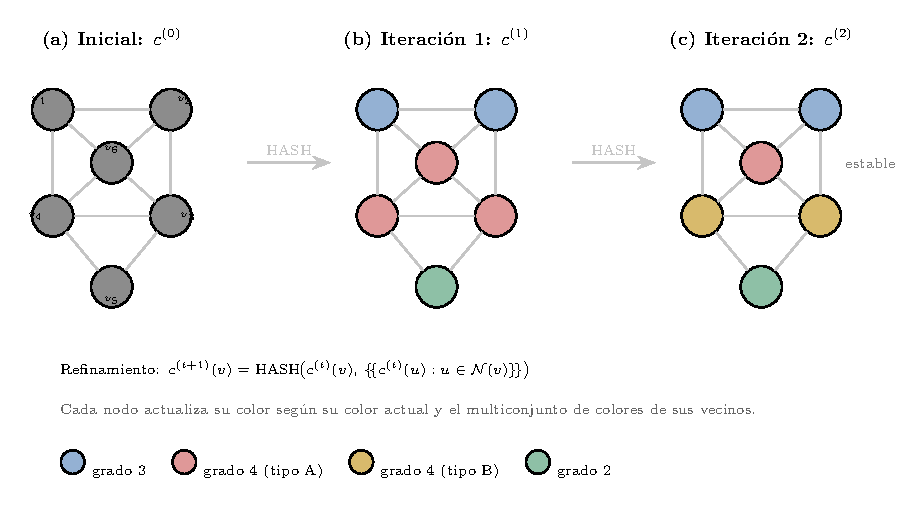
\includegraphics[width=\textwidth]{images/weisfeiler_leman.pdf}
\caption[Refinamiento de colores Weisfeiler-Leman]{Ejemplo del test de refinamiento de colores 1-WL sobre un grafo de 6 nodos. (a) Coloración inicial uniforme. (b) Tras la primera iteración, los nodos se distinguen por grado: azul (grado~3), rojo (grado~4), verde (grado~2). (c) La segunda iteración refina según el multiconjunto de colores vecinos: $v_3$ y $v_4$ (amarillo) se separan de $v_6$ (rojo) porque sus vecindarios tienen composiciones de colores distintas.}
\label{fig:weisfeiler_leman}
\end{figure}

La conexión profunda entre el test WL y las redes de grafos fue establecida rigurosamente por~\citet{xu2019how} y~\citet{morris2019weisfeiler}:

\begin{theorem}[Equivalencia WL-MPNN]\label{thm:wl_mpnn_equivalencia}
Sea $\mathcal{G}$ una clase de grafos y sea $\mathcal{A}$ una \gls{MPNN} con funciones de agregación y actualización inyectivas. Entonces:
\begin{enumerate}
    \item \textbf{Cota superior}: $\mathcal{A}$ no puede distinguir grafos que son WL-equivalentes. Es decir, si $G_1 \equiv_{\mathrm{WL}} G_2$, entonces $\mathcal{A}(G_1) = \mathcal{A}(G_2)$.

    \item \textbf{Optimalidad}: Existe una \gls{MPNN} (específicamente, una Graph Isomorphism Network o GIN) que es \textit{tan expresiva como} el test WL. Es decir, si $G_1 \not\equiv_{\mathrm{WL}} G_2$, existe una configuración de pesos tal que $\mathcal{A}(G_1) \neq \mathcal{A}(G_2)$.
\end{enumerate}
\end{theorem}

\begin{proof}[Sketch de demostración]
La idea clave es la correspondencia estructural entre una iteración del algoritmo WL y una capa de una \gls{MPNN}:

\textbf{WL $\rightarrow$ MPNN}: El refinamiento de WL $c^{(t+1)}(v) = \mathrm{HASH}(c^{(t)}(v), \{\{c^{(t)}(u)\}\})$ se mapea directamente a una capa de mensaje-agregación-actualización:
\[
h_v^{(t+1)} = \phi\left(h_v^{(t)}, \bigoplus_{u \in \mathcal{N}(v)} \psi(h_u^{(t)})\right)
\]
Si $\phi$ y $\oplus$ son suficientemente expresivas (por ejemplo, suma sobre embeddings únicos seguida de MLP), reproducen exactamente el comportamiento de $\mathrm{HASH}$.

\textbf{MPNN $\rightarrow$ WL}: Recíprocamente, si dos grafos son WL-equivalentes, tienen la misma secuencia de particiones de colores. Dado que las \glspl{MPNN} solo pueden agregar información del vecindario, no pueden ``romper'' la simetría que el test WL preserva.

La demostración completa requiere mostrar que el agregador de suma sobre embeddings suficientemente únicos es inyectivo, lo cual se establece mediante el Teorema de Aproximación Universal para conjuntos~\citep{zaheer2017deepsets}.
\end{proof}

\begin{example}[Grafos no isomorfos indistinguibles por WL]\label{ex:grafos_wl_indistinguibles}
El ejemplo más simple de grafos no isomorfos que el test 1-WL no puede distinguir son los grafos regulares de mismo grado y tamaño:

Consideremos dos grafos hexagonales:
\begin{itemize}
    \item $G_1$: Un ciclo de 6 nodos (hexágono): $C_6$
    \item $G_2$: Dos triángulos disjuntos: $K_3 \sqcup K_3$
\end{itemize}

Ambos grafos tienen 6 nodos, 6 aristas, y todos los nodos tienen grado 2. El algoritmo WL asigna:
\begin{enumerate}
    \item Iteración 0: Todos los nodos reciben el mismo color inicial $c^{(0)} = 1$.
    \item Iteración 1: Cada nodo ve vecinos con color 1, multiconjunto $\{\{1, 1\}\}$. Nuevo color: $c^{(1)} = \mathrm{HASH}(1, \{\{1,1\}\}) = 2$ para todos.
    \item Convergencia: La partición no cambia. Histograma final: $\mathbf{h}(G_1) = \mathbf{h}(G_2) = (6)$.
\end{enumerate}

Sin embargo, $G_1 \not\cong G_2$: el ciclo $C_6$ es conexo mientras que $K_3 \sqcup K_3$ tiene dos componentes conexas. Esta limitación demuestra que las \glspl{MPNN} estándar no pueden detectar la conectividad global de grafos regulares.

\textbf{Implicación para GDL}: Si una tarea requiere distinguir moléculas con estructuras globales similares pero conectividades diferentes (por ejemplo, isómeros estructurales), las \glspl{MPNN} estándar pueden fallar sistemáticamente.
\end{example}

\subsubsection{Sobre-suavizado: Análisis Espectral}\label{subsubsec:oversmoothing}

El \autoref{thm:wl_mpnn_equivalencia} delimita qué grafos pueden distinguir las \glspl{MPNN}, pero no dice nada sobre qué sucede cuando apilamos muchas capas de paso de mensajes. La respuesta, conocida como \textit{\gls{oversmoothing}}~\citep{li2018deeper}, es que las representaciones de los nodos convergen a un valor uniforme, perdiendo toda capacidad discriminativa. Este fenómeno admite una explicación espectral elegante que conecta directamente con las herramientas desarrolladas en la \autoref{subsec:analisis_espectral_grafos_gdl}.

\begin{definition}[Energía de Dirichlet en grafos]\label{def:energia_dirichlet_grafos}
	Sea $\mathcal{G} = (V, E)$ un grafo con Laplaciano $L_G$ y sea $H \in \mathbb{R}^{n \times d}$ una matriz de características de nodos ($n = |V|$, $d$ canales). La \textit{energía de Dirichlet} de $H$ es
	\[
		E(H) = \operatorname{tr}(H^T L_G H) = \sum_{c=1}^{d} \mathbf{h}_c^T L_G \mathbf{h}_c = \sum_{c=1}^{d} \sum_{(i,j) \in E} W_{ij}(h_{ic} - h_{jc})^2,
	\]
	donde $\mathbf{h}_c$ denota la $c$-ésima columna de $H$.
\end{definition}

La última igualdad se sigue de la forma cuadrática de la \autoref{prop:propiedades_algebraicas_laplaciano}. La energía de Dirichlet mide la variación total de las señales $H$ sobre el grafo: $E(H) = 0$ si y solo si $H$ es constante en cada componente conexa. Esta es la versión discreta de la energía de Dirichlet mencionada en la \autoref{subsec:analisis_espectral_grafos_gdl}.

\begin{proposition}[MPNN lineal como difusión discreta]\label{prop:mpnn_difusion}
	Consideremos una \gls{MPNN} (\autoref{def:mpnn_unificador}) con agregación por media y sin no linealidad:
	\[
		h_v^{(\ell+1)} = (1 - \alpha) h_v^{(\ell)} + \alpha \sum_{u \in \mathcal{N}(v)} \frac{h_u^{(\ell)}}{\deg(v)},
	\]
	con $\alpha \in (0, 1]$. Sea $\tilde{L} = D^{-1}L_G = I - D^{-1}A$ el Laplaciano por random walk, que comparte espectro con el Laplaciano normalizado simétrico de la \autoref{def:laplaciano_normalizado}. Entonces la actualización se escribe matricialmente como
	\begin{equation}\label{eq:difusion_discreta}
		H^{(\ell+1)} = (I - \alpha \tilde{L})\, H^{(\ell)}.
	\end{equation}
\end{proposition}

\begin{proof}
	Para cada nodo $v$, la regla de actualización es:
	\begin{align*}
		h_v^{(\ell+1)} &= (1-\alpha) h_v^{(\ell)} + \alpha \sum_{u \sim v} \frac{h_u^{(\ell)}}{\deg(v)} = h_v^{(\ell)} - \alpha\left(h_v^{(\ell)} - \sum_{u \sim v} \frac{h_u^{(\ell)}}{\deg(v)}\right)\\
		&= h_v^{(\ell)} - \alpha (D^{-1}L_G\, H^{(\ell)})_v = h_v^{(\ell)} - \alpha (\tilde{L}\, H^{(\ell)})_v,
	\end{align*}
	donde usamos que $\tilde{L} = D^{-1}L_G = I - D^{-1}A$ y que $(D^{-1}A H)_v = \sum_{u \sim v} h_u / \deg(v)$.
\end{proof}

La ecuación~\eqref{eq:difusion_discreta} es la discretización temporal de la ecuación del calor $\partial_t H = -\alpha \tilde{L} H$ en el grafo. Iterando $\ell$ capas, $H^{(\ell)} = (I - \alpha \tilde{L})^\ell H^{(0)}$, que difunde las señales progresivamente.

\begin{theorem}[Convergencia exponencial del sobre-suavizado]\label{thm:oversmoothing_convergencia}
	Sea $\mathcal{G}$ un grafo conexo con valores propios del Laplaciano normalizado $0 = \lambda_1 < \lambda_2 \leq \cdots \leq \lambda_n$ (\autoref{prop:propiedades_espectrales_laplaciano_grafos}) y $\alpha \in (0, 1/\lambda_n)$. Entonces la energía de Dirichlet de las representaciones tras $\ell$ capas de la \gls{MPNN} lineal satisface
	\begin{equation}\label{eq:oversmoothing_bound}
		E\bigl(H^{(\ell)}\bigr) \leq (1 - \alpha\lambda_2)^{2\ell}\, E\bigl(H^{(0)}\bigr).
	\end{equation}
	En particular, $E(H^{(\ell)}) \to 0$ exponencialmente cuando $\ell \to \infty$: todas las representaciones convergen a un mismo vector.
\end{theorem}

\begin{proof}
	Sea $\{u_k\}_{k=1}^n$ la base ortonormal de autovectores de $L_{\mathrm{sym}} = D^{-1/2} L_G D^{-1/2}$ con autovalores $\lambda_k$ (\autoref{def:transformada_fourier_grafos}). Definimos $\mathbf{f}_c = D^{1/2}\mathbf{h}_c$ para cada columna de $H$, de modo que $\mathbf{h}_c^T L_G \mathbf{h}_c = \mathbf{f}_c^T L_{\mathrm{sym}} \mathbf{f}_c$. La transformada de Fourier descompone $\mathbf{f}_c = \sum_{k=1}^n \hat{f}_{c,k}\, u_k$.

	El operador de difusión satisface $D^{1/2}(I - \alpha \tilde{L})D^{-1/2} = I - \alpha L_{\mathrm{sym}}$, que tiene autovalores $1 - \alpha\lambda_k$. Tras $\ell$ iteraciones, los coeficientes espectrales de $\mathbf{f}_c^{(\ell)} = D^{1/2}\mathbf{h}_c^{(\ell)}$ se escalan como $(1-\alpha\lambda_k)^\ell \hat{f}_{c,k}$.

	La energía de Dirichlet en el dominio espectral es (\autoref{thm:interpretacion_frecuencial_autovectores}):
	\[
		E(H^{(\ell)}) = \sum_{c=1}^d \mathbf{f}_c^{(\ell)T} L_{\mathrm{sym}} \mathbf{f}_c^{(\ell)} = \sum_{c=1}^d \sum_{k=2}^n \lambda_k (1-\alpha\lambda_k)^{2\ell} |\hat{f}_{c,k}|^2,
	\]
	donde el término $k=1$ desaparece porque $\lambda_1 = 0$. Como $\alpha < 1/\lambda_n$, se tiene $|1-\alpha\lambda_k| < 1$ para $k \geq 2$, y en particular $|1-\alpha\lambda_k| \leq 1-\alpha\lambda_2$ para todo $k \geq 2$ (el máximo se alcanza en $\lambda_2$, la frecuencia más baja no trivial). Por tanto:
	\[
		E(H^{(\ell)}) \leq (1-\alpha\lambda_2)^{2\ell} \sum_{c=1}^d \sum_{k=2}^n \lambda_k |\hat{f}_{c,k}|^2
		= (1-\alpha\lambda_2)^{2\ell}\, E(H^{(0)}).
	\]
	Como $0 < \alpha\lambda_2 < 1$, el factor $(1-\alpha\lambda_2)^{2\ell} \to 0$ exponencialmente.
\end{proof}

\begin{remark}[Interpretación geométrica del sobre-suavizado]\label{rem:oversmoothing_geometrico}
	La tasa de convergencia $(1-\alpha\lambda_2)^{2\ell}$ está controlada por el \textbf{gap espectral} $\lambda_2$, el segundo autovalor del Laplaciano. Grafos con $\lambda_2$ grande (como los expansores) convergen más rápido al estado uniforme, mientras que grafos poco conectados ($\lambda_2 \approx 0$) preservan mejor la diversidad de representaciones. Esta es la versión discreta exacta de la difusión del calor en variedades riemannianas (\autoref{rem:laplace_beltrami_gdl}), donde el gap espectral del operador de Laplace-Beltrami controla la tasa de mezclado.

	Entre las estrategias para mitigar el \gls{oversmoothing} destacan las conexiones residuales (que preservan la señal original), la normalización por capas y los enfoques topológicos como Neural Sheaf Diffusion~\citep{bodnar2022neural}, donde se reemplaza la difusión escalar por una difusión en haces (sheaves) que permite a cada arista transportar información en espacios vectoriales diferentes.
\end{remark}

\subsubsection{Sobre-compresión: Cuellos de Botella Topológicos}\label{subsubsec:oversquashing}

Si el \gls{oversmoothing} surge de la pérdida de señal de alta frecuencia, el fenómeno complementario de \textit{\gls{oversquashing}} es la incapacidad de propagar información a larga distancia. Intuitivamente, la información de un nodo lejano debe comprimirse exponencialmente para ``pasar'' por los cuellos de botella del grafo.

\begin{definition}[Sensibilidad Jacobiana de una MPNN]\label{def:sensibilidad_mpnn}
	Sea una \gls{MPNN} con representaciones $h_v^{(\ell)} \in \mathbb{R}^d$. La \textit{sensibilidad} del nodo $v$ respecto al nodo $u$ tras $\ell$ capas es
	\[
		S_{vu}^{(\ell)} = \left\|\frac{\partial h_v^{(\ell)}}{\partial h_u^{(0)}}\right\|,
	\]
	donde la norma es la norma de operador de la matriz Jacobiana $\partial h_v^{(\ell)} / \partial h_u^{(0)} \in \mathbb{R}^{d \times d}$.
\end{definition}

Si $S_{vu}^{(\ell)} \approx 0$, el nodo $v$ es esencialmente insensible a la entrada del nodo $u$: cualquier información que $u$ porte se ha perdido durante la propagación.

\begin{proposition}[Decaimiento exponencial de la sensibilidad]\label{prop:oversquashing_exponencial}
	Sea una \gls{MPNN} con funciones de mensaje y actualización Lipschitz con constantes $c_M$ y $c_U$ respectivamente, y sea $\hat{A} = D^{-1}A$ la matriz de transición del random walk en $\mathcal{G}$. Entonces para cualesquiera nodos $v, u \in V$:
	\begin{equation}\label{eq:oversquashing_bound}
		S_{vu}^{(\ell)} \leq (c_U \cdot c_M)^\ell\, [\hat{A}^\ell]_{vu}.
	\end{equation}
	En particular, si $d_\mathcal{G}(v, u) > \ell$ (\autoref{def:distancia_geodesica_grafo}), entonces $[\hat{A}^\ell]_{vu} = 0$ y la sensibilidad es exactamente cero.
\end{proposition}

\begin{proof}[Sketch de demostración]
	Procedemos por inducción sobre $\ell$. Para $\ell = 1$ y nodos $v \neq u$,
	como $h_v^{(1)} = U(h_v^{(0)}, m_v^{(1)})$, la regla de la cadena completa es
	\[
		\frac{\partial h_v^{(1)}}{\partial h_u^{(0)}}
		= \frac{\partial U}{\partial h_v^{(0)}}
		  \cdot \underbrace{\frac{\partial h_v^{(0)}}{\partial h_u^{(0)}}}_{=\,0 \text{ si } v \neq u}
		+ \frac{\partial U}{\partial m_v}
		  \cdot \frac{\partial m_v}{\partial h_u^{(0)}}
		= \frac{\partial U}{\partial m_v}
		  \cdot \frac{\partial m_v}{\partial h_u^{(0)}}.
	\]
	El segundo factor es no nulo solo si $u \in \mathcal{N}(v)$, en cuyo caso
	la constante de Lipschitz de $M$ contribuye $c_M$ y la normalización por
	grado aporta el factor $1/\deg(v) = [\hat{A}]_{vu}$. Así
	$S_{vu}^{(1)} \leq c_U c_M [\hat{A}]_{vu}$.

	Para el paso inductivo, aplicamos la regla de la cadena multivariable:
	\[
		\frac{\partial h_v^{(\ell+1)}}{\partial h_u^{(0)}} = \sum_{w \in \mathcal{N}(v) \cup \{v\}} \frac{\partial h_v^{(\ell+1)}}{\partial h_w^{(\ell)}} \cdot \frac{\partial h_w^{(\ell)}}{\partial h_u^{(0)}}.
	\]
	Acotando cada factor por las constantes de Lipschitz y usando la hipótesis inductiva para $\partial h_w^{(\ell)} / \partial h_u^{(0)}$, obtenemos el producto matricial $\hat{A}^{\ell+1}$ que registra todos los caminos de longitud $\ell+1$ de $u$ a $v$.
\end{proof}

\begin{remark}[Curvatura y sobre-compresión]\label{rem:curvatura_oversquashing}
	La cota~\eqref{eq:oversquashing_bound} revela que la topología del grafo, codificada en $\hat{A}^\ell$, es el factor determinante del \gls{oversquashing}. \citet{topping2022understanding} formalizan esta conexión mediante la \textbf{curvatura de Ricci discreta} (Ollivier): aristas $(u,v)$ con curvatura de Ricci negativa corresponden a cuellos de botella donde $[\hat{A}^\ell]_{vu}$ decae rápidamente. Esta es la versión discreta de la ecuación de Jacobi en geometría riemanniana (\autoref{rem:significado_curvatura}): la curvatura seccional negativa hace que las geodésicas diverjan, reduciendo el ``volumen de información'' que puede propagarse. Topping et al. proponen el \textit{rewiring} del grafo mediante flujo de Ricci, añadiendo aristas en regiones de curvatura negativa para aliviar los cuellos de botella, un ejemplo de cómo la geometría diferencial prescribe soluciones a problemas de las \glspl{GNN}.
\end{remark}

\subsubsection{Jerarquía k-WL y Extensiones}\label{subsubsec:jerarquia_kwl}

El \autoref{thm:wl_mpnn_equivalencia} establece que las \glspl{MPNN} son tan expresivas como el test 1-WL, que opera sobre nodos individuales. Una extensión natural es considerar tests de orden superior que operen sobre tuplas de nodos.

\begin{definition}[Test de Weisfeiler-Leman de orden $k$]\label{def:k_wl}
	El \textit{test $k$-\gls{WL}} opera sobre $k$-tuplas de nodos $\bar{v} = (v_1, \ldots, v_k) \in V^k$ \citep{morris2019weisfeiler}. Se define una coloración inicial $c^{(0)}(\bar{v})$ basada en el tipo de isomorfismo de la subtupla, y el refinamiento iterativo:
	\[
		c^{(t+1)}(\bar{v}) = \mathrm{HASH}\!\left(c^{(t)}(\bar{v}),\, \bigl\{\!\!\bigl\{ \bigl(c^{(t)}(\bar{v}[w/1]), \ldots, c^{(t)}(\bar{v}[w/k])\bigr) : w \in V \bigr\}\!\!\bigr\}\right),
	\]
	donde $\bar{v}[w/i]$ denota la tupla obtenida al reemplazar la $i$-ésima componente de $\bar{v}$ por $w$.
\end{definition}

\begin{proposition}[Jerarquía estricta de expresividad]\label{prop:jerarquia_kwl}
	Los tests de Weisfeiler-Leman forman una jerarquía estrictamente creciente en poder expresivo:
	\[
		1\text{-WL} \subsetneq 2\text{-WL} \subsetneq 3\text{-WL} \subsetneq \cdots
	\]
	Es decir, para cada $k \geq 1$ existen grafos que $k$-WL no distingue pero $(k+1)$-WL sí. La complejidad computacional del test $k$-WL es $O(n^k \log n)$ por iteración, donde $n = |V|$.
\end{proposition}

\begin{proof}
	La demostración de la separación estricta requiere técnicas de lógica finita de modelos (en particular, la conexión con la lógica $C^k$ de Immerman-Lander) y excede el alcance de esta tesis; véase~\citet{morris2019weisfeiler} para los detalles. La complejidad $O(n^k \log n)$ se sigue directamente del refinamiento iterativo: hay $n^k$ tuplas, cada iteración requiere inspeccionar $n$ sustituciones por tupla, y la estabilización ocurre en a lo sumo $O(n^k)$ iteraciones con coste $O(\log n)$ del hash.
\end{proof}

Existen diversas estrategias para superar la barrera 1-WL sin incurrir en el coste exponencial de $k$-WL:
\begin{itemize}
	\item \textbf{Paso de mensajes simplicial}: Como muestra la \autoref{prop:expresividad_simplicial}, operar sobre complejos simpliciales ($k$-cadenas) permite superar 1-WL incorporando información topológica de orden superior.
	\item \textbf{Codificaciones estructurales}: Añadir codificaciones posicionales basadas en autovectores del Laplaciano (\autoref{def:transformada_fourier_grafos}) o random walks rompe la simetría de los nodos.
	\item \textbf{Graph Transformers espectrales}: Arquitecturas como~\citet{kreuzer2021spectral} combinan atención global con codificaciones espectrales, conectando las ideas de la \autoref{subsec:analisis_espectral_grafos_gdl} con los mecanismos de atención del \autoref{ch:attention}.
\end{itemize}

\medskip

Las tres limitaciones analizadas (\gls{oversmoothing}, \gls{oversquashing} y barrera WL) son manifestaciones del carácter fundamentalmente \textbf{local} del paso de mensajes: cada capa solo propaga información un salto. El \gls{oversmoothing} muestra que demasiadas capas destruyen la señal discriminativa; el \gls{oversquashing} muestra que pocas capas impiden la comunicación a larga distancia; y la barrera WL muestra que ciertos patrones globales son indetectables localmente. Las herramientas geométricas desarrolladas en este capítulo (análisis espectral, curvatura discreta, topología de orden superior) no solo \textit{diagnostican} estas limitaciones sino que \textit{prescriben} soluciones concretas.

Desde esta perspectiva, podemos sintetizar el marco unificador que emerge del análisis precedente. La perspectiva unificadora del \gls{GDL} revela una progresión natural en la sofisticación geométrica de las arquitecturas neuronales: las \glspl{ANN} operan en espacios euclidianos con simetrías triviales; las \glspl{CNN} introducen \textbf{bias inductivo espacial} mediante localidad y equivarianza traslacional; los \glspl{Transformer} generalizan esto mediante \textbf{conectividad adaptativa global}, donde la atención implementa paso de mensajes con pesos dinámicos; y este paradigma se extiende naturalmente a grafos arbitrarios con topologías complejas.

Este marco teórico es predictivo, no meramente descriptivo: sugiere principios de diseño para nuevas arquitecturas híbridas basados en los fundamentos geométricos establecidos. Los Capítulos~\ref{ch:cnn} y~\ref{ch:attention} profundizan en estas arquitecturas desde sus perspectivas geométricas específicas, proporcionando los fundamentos matemáticos completos para convoluciones equivariantes y mecanismos de atención geométrica. La geometría no es opcional en el Deep Learning: es el principio organizador fundamental que determina qué arquitecturas son efectivas para qué tipos de datos y problemas.
